\documentclass[11pt]{article}

    \usepackage[breakable]{tcolorbox}
    \usepackage{parskip} % Stop auto-indenting (to mimic markdown behaviour)
    
    \usepackage{iftex}
    \ifPDFTeX
    	\usepackage[T1]{fontenc}
    	\usepackage{mathpazo}
    \else
    	\usepackage{fontspec}
    \fi

    % Basic figure setup, for now with no caption control since it's done
    % automatically by Pandoc (which extracts ![](path) syntax from Markdown).
    \usepackage{graphicx}
    % Maintain compatibility with old templates. Remove in nbconvert 6.0
    \let\Oldincludegraphics\includegraphics
    % Ensure that by default, figures have no caption (until we provide a
    % proper Figure object with a Caption API and a way to capture that
    % in the conversion process - todo).
    \usepackage{caption}
    \DeclareCaptionFormat{nocaption}{}
    \captionsetup{format=nocaption,aboveskip=0pt,belowskip=0pt}

    \usepackage{float}
    \floatplacement{figure}{H} % forces figures to be placed at the correct location
    \usepackage{xcolor} % Allow colors to be defined
    \usepackage{enumerate} % Needed for markdown enumerations to work
    \usepackage{geometry} % Used to adjust the document margins
    \usepackage{amsmath} % Equations
    \usepackage{amssymb} % Equations
    \usepackage{textcomp} % defines textquotesingle
    % Hack from http://tex.stackexchange.com/a/47451/13684:
    \AtBeginDocument{%
        \def\PYZsq{\textquotesingle}% Upright quotes in Pygmentized code
    }
    \usepackage{upquote} % Upright quotes for verbatim code
    \usepackage{eurosym} % defines \euro
    \usepackage[mathletters]{ucs} % Extended unicode (utf-8) support
    \usepackage{fancyvrb} % verbatim replacement that allows latex
    \usepackage{grffile} % extends the file name processing of package graphics 
                         % to support a larger range
    \makeatletter % fix for old versions of grffile with XeLaTeX
    \@ifpackagelater{grffile}{2019/11/01}
    {
      % Do nothing on new versions
    }
    {
      \def\Gread@@xetex#1{%
        \IfFileExists{"\Gin@base".bb}%
        {\Gread@eps{\Gin@base.bb}}%
        {\Gread@@xetex@aux#1}%
      }
    }
    \makeatother
    \usepackage[Export]{adjustbox} % Used to constrain images to a maximum size
    \adjustboxset{max size={0.9\linewidth}{0.9\paperheight}}

    % The hyperref package gives us a pdf with properly built
    % internal navigation ('pdf bookmarks' for the table of contents,
    % internal cross-reference links, web links for URLs, etc.)
    \usepackage{hyperref}
    % The default LaTeX title has an obnoxious amount of whitespace. By default,
    % titling removes some of it. It also provides customization options.
    \usepackage{titling}
    \usepackage{longtable} % longtable support required by pandoc >1.10
    \usepackage{booktabs}  % table support for pandoc > 1.12.2
    \usepackage[inline]{enumitem} % IRkernel/repr support (it uses the enumerate* environment)
    \usepackage[normalem]{ulem} % ulem is needed to support strikethroughs (\sout)
                                % normalem makes italics be italics, not underlines
    \usepackage{mathrsfs}
    

    
    % Colors for the hyperref package
    \definecolor{urlcolor}{rgb}{0,.145,.698}
    \definecolor{linkcolor}{rgb}{.71,0.21,0.01}
    \definecolor{citecolor}{rgb}{.12,.54,.11}

    % ANSI colors
    \definecolor{ansi-black}{HTML}{3E424D}
    \definecolor{ansi-black-intense}{HTML}{282C36}
    \definecolor{ansi-red}{HTML}{E75C58}
    \definecolor{ansi-red-intense}{HTML}{B22B31}
    \definecolor{ansi-green}{HTML}{00A250}
    \definecolor{ansi-green-intense}{HTML}{007427}
    \definecolor{ansi-yellow}{HTML}{DDB62B}
    \definecolor{ansi-yellow-intense}{HTML}{B27D12}
    \definecolor{ansi-blue}{HTML}{208FFB}
    \definecolor{ansi-blue-intense}{HTML}{0065CA}
    \definecolor{ansi-magenta}{HTML}{D160C4}
    \definecolor{ansi-magenta-intense}{HTML}{A03196}
    \definecolor{ansi-cyan}{HTML}{60C6C8}
    \definecolor{ansi-cyan-intense}{HTML}{258F8F}
    \definecolor{ansi-white}{HTML}{C5C1B4}
    \definecolor{ansi-white-intense}{HTML}{A1A6B2}
    \definecolor{ansi-default-inverse-fg}{HTML}{FFFFFF}
    \definecolor{ansi-default-inverse-bg}{HTML}{000000}

    % common color for the border for error outputs.
    \definecolor{outerrorbackground}{HTML}{FFDFDF}

    % commands and environments needed by pandoc snippets
    % extracted from the output of `pandoc -s`
    \providecommand{\tightlist}{%
      \setlength{\itemsep}{0pt}\setlength{\parskip}{0pt}}
    \DefineVerbatimEnvironment{Highlighting}{Verbatim}{commandchars=\\\{\}}
    % Add ',fontsize=\small' for more characters per line
    \newenvironment{Shaded}{}{}
    \newcommand{\KeywordTok}[1]{\textcolor[rgb]{0.00,0.44,0.13}{\textbf{{#1}}}}
    \newcommand{\DataTypeTok}[1]{\textcolor[rgb]{0.56,0.13,0.00}{{#1}}}
    \newcommand{\DecValTok}[1]{\textcolor[rgb]{0.25,0.63,0.44}{{#1}}}
    \newcommand{\BaseNTok}[1]{\textcolor[rgb]{0.25,0.63,0.44}{{#1}}}
    \newcommand{\FloatTok}[1]{\textcolor[rgb]{0.25,0.63,0.44}{{#1}}}
    \newcommand{\CharTok}[1]{\textcolor[rgb]{0.25,0.44,0.63}{{#1}}}
    \newcommand{\StringTok}[1]{\textcolor[rgb]{0.25,0.44,0.63}{{#1}}}
    \newcommand{\CommentTok}[1]{\textcolor[rgb]{0.38,0.63,0.69}{\textit{{#1}}}}
    \newcommand{\OtherTok}[1]{\textcolor[rgb]{0.00,0.44,0.13}{{#1}}}
    \newcommand{\AlertTok}[1]{\textcolor[rgb]{1.00,0.00,0.00}{\textbf{{#1}}}}
    \newcommand{\FunctionTok}[1]{\textcolor[rgb]{0.02,0.16,0.49}{{#1}}}
    \newcommand{\RegionMarkerTok}[1]{{#1}}
    \newcommand{\ErrorTok}[1]{\textcolor[rgb]{1.00,0.00,0.00}{\textbf{{#1}}}}
    \newcommand{\NormalTok}[1]{{#1}}
    
    % Additional commands for more recent versions of Pandoc
    \newcommand{\ConstantTok}[1]{\textcolor[rgb]{0.53,0.00,0.00}{{#1}}}
    \newcommand{\SpecialCharTok}[1]{\textcolor[rgb]{0.25,0.44,0.63}{{#1}}}
    \newcommand{\VerbatimStringTok}[1]{\textcolor[rgb]{0.25,0.44,0.63}{{#1}}}
    \newcommand{\SpecialStringTok}[1]{\textcolor[rgb]{0.73,0.40,0.53}{{#1}}}
    \newcommand{\ImportTok}[1]{{#1}}
    \newcommand{\DocumentationTok}[1]{\textcolor[rgb]{0.73,0.13,0.13}{\textit{{#1}}}}
    \newcommand{\AnnotationTok}[1]{\textcolor[rgb]{0.38,0.63,0.69}{\textbf{\textit{{#1}}}}}
    \newcommand{\CommentVarTok}[1]{\textcolor[rgb]{0.38,0.63,0.69}{\textbf{\textit{{#1}}}}}
    \newcommand{\VariableTok}[1]{\textcolor[rgb]{0.10,0.09,0.49}{{#1}}}
    \newcommand{\ControlFlowTok}[1]{\textcolor[rgb]{0.00,0.44,0.13}{\textbf{{#1}}}}
    \newcommand{\OperatorTok}[1]{\textcolor[rgb]{0.40,0.40,0.40}{{#1}}}
    \newcommand{\BuiltInTok}[1]{{#1}}
    \newcommand{\ExtensionTok}[1]{{#1}}
    \newcommand{\PreprocessorTok}[1]{\textcolor[rgb]{0.74,0.48,0.00}{{#1}}}
    \newcommand{\AttributeTok}[1]{\textcolor[rgb]{0.49,0.56,0.16}{{#1}}}
    \newcommand{\InformationTok}[1]{\textcolor[rgb]{0.38,0.63,0.69}{\textbf{\textit{{#1}}}}}
    \newcommand{\WarningTok}[1]{\textcolor[rgb]{0.38,0.63,0.69}{\textbf{\textit{{#1}}}}}
    
    
    % Define a nice break command that doesn't care if a line doesn't already
    % exist.
    \def\br{\hspace*{\fill} \\* }
    % Math Jax compatibility definitions
    \def\gt{>}
    \def\lt{<}
    \let\Oldtex\TeX
    \let\Oldlatex\LaTeX
    \renewcommand{\TeX}{\textrm{\Oldtex}}
    \renewcommand{\LaTeX}{\textrm{\Oldlatex}}
    % Document parameters
    % Document title
    \title{From Synchrotron Microtomography to CAD Models using
Optimisation and Fast X-ray Simulation on
GPU: Registration of Tungsten Fibres on XCT}
    
\author{Franck P. Vidal and Jean-Michel L\'etang}

    
    
% Pygments definitions
\makeatletter
\def\PY@reset{\let\PY@it=\relax \let\PY@bf=\relax%
    \let\PY@ul=\relax \let\PY@tc=\relax%
    \let\PY@bc=\relax \let\PY@ff=\relax}
\def\PY@tok#1{\csname PY@tok@#1\endcsname}
\def\PY@toks#1+{\ifx\relax#1\empty\else%
    \PY@tok{#1}\expandafter\PY@toks\fi}
\def\PY@do#1{\PY@bc{\PY@tc{\PY@ul{%
    \PY@it{\PY@bf{\PY@ff{#1}}}}}}}
\def\PY#1#2{\PY@reset\PY@toks#1+\relax+\PY@do{#2}}

\@namedef{PY@tok@w}{\def\PY@tc##1{\textcolor[rgb]{0.73,0.73,0.73}{##1}}}
\@namedef{PY@tok@c}{\let\PY@it=\textit\def\PY@tc##1{\textcolor[rgb]{0.25,0.50,0.50}{##1}}}
\@namedef{PY@tok@cp}{\def\PY@tc##1{\textcolor[rgb]{0.74,0.48,0.00}{##1}}}
\@namedef{PY@tok@k}{\let\PY@bf=\textbf\def\PY@tc##1{\textcolor[rgb]{0.00,0.50,0.00}{##1}}}
\@namedef{PY@tok@kp}{\def\PY@tc##1{\textcolor[rgb]{0.00,0.50,0.00}{##1}}}
\@namedef{PY@tok@kt}{\def\PY@tc##1{\textcolor[rgb]{0.69,0.00,0.25}{##1}}}
\@namedef{PY@tok@o}{\def\PY@tc##1{\textcolor[rgb]{0.40,0.40,0.40}{##1}}}
\@namedef{PY@tok@ow}{\let\PY@bf=\textbf\def\PY@tc##1{\textcolor[rgb]{0.67,0.13,1.00}{##1}}}
\@namedef{PY@tok@nb}{\def\PY@tc##1{\textcolor[rgb]{0.00,0.50,0.00}{##1}}}
\@namedef{PY@tok@nf}{\def\PY@tc##1{\textcolor[rgb]{0.00,0.00,1.00}{##1}}}
\@namedef{PY@tok@nc}{\let\PY@bf=\textbf\def\PY@tc##1{\textcolor[rgb]{0.00,0.00,1.00}{##1}}}
\@namedef{PY@tok@nn}{\let\PY@bf=\textbf\def\PY@tc##1{\textcolor[rgb]{0.00,0.00,1.00}{##1}}}
\@namedef{PY@tok@ne}{\let\PY@bf=\textbf\def\PY@tc##1{\textcolor[rgb]{0.82,0.25,0.23}{##1}}}
\@namedef{PY@tok@nv}{\def\PY@tc##1{\textcolor[rgb]{0.10,0.09,0.49}{##1}}}
\@namedef{PY@tok@no}{\def\PY@tc##1{\textcolor[rgb]{0.53,0.00,0.00}{##1}}}
\@namedef{PY@tok@nl}{\def\PY@tc##1{\textcolor[rgb]{0.63,0.63,0.00}{##1}}}
\@namedef{PY@tok@ni}{\let\PY@bf=\textbf\def\PY@tc##1{\textcolor[rgb]{0.60,0.60,0.60}{##1}}}
\@namedef{PY@tok@na}{\def\PY@tc##1{\textcolor[rgb]{0.49,0.56,0.16}{##1}}}
\@namedef{PY@tok@nt}{\let\PY@bf=\textbf\def\PY@tc##1{\textcolor[rgb]{0.00,0.50,0.00}{##1}}}
\@namedef{PY@tok@nd}{\def\PY@tc##1{\textcolor[rgb]{0.67,0.13,1.00}{##1}}}
\@namedef{PY@tok@s}{\def\PY@tc##1{\textcolor[rgb]{0.73,0.13,0.13}{##1}}}
\@namedef{PY@tok@sd}{\let\PY@it=\textit\def\PY@tc##1{\textcolor[rgb]{0.73,0.13,0.13}{##1}}}
\@namedef{PY@tok@si}{\let\PY@bf=\textbf\def\PY@tc##1{\textcolor[rgb]{0.73,0.40,0.53}{##1}}}
\@namedef{PY@tok@se}{\let\PY@bf=\textbf\def\PY@tc##1{\textcolor[rgb]{0.73,0.40,0.13}{##1}}}
\@namedef{PY@tok@sr}{\def\PY@tc##1{\textcolor[rgb]{0.73,0.40,0.53}{##1}}}
\@namedef{PY@tok@ss}{\def\PY@tc##1{\textcolor[rgb]{0.10,0.09,0.49}{##1}}}
\@namedef{PY@tok@sx}{\def\PY@tc##1{\textcolor[rgb]{0.00,0.50,0.00}{##1}}}
\@namedef{PY@tok@m}{\def\PY@tc##1{\textcolor[rgb]{0.40,0.40,0.40}{##1}}}
\@namedef{PY@tok@gh}{\let\PY@bf=\textbf\def\PY@tc##1{\textcolor[rgb]{0.00,0.00,0.50}{##1}}}
\@namedef{PY@tok@gu}{\let\PY@bf=\textbf\def\PY@tc##1{\textcolor[rgb]{0.50,0.00,0.50}{##1}}}
\@namedef{PY@tok@gd}{\def\PY@tc##1{\textcolor[rgb]{0.63,0.00,0.00}{##1}}}
\@namedef{PY@tok@gi}{\def\PY@tc##1{\textcolor[rgb]{0.00,0.63,0.00}{##1}}}
\@namedef{PY@tok@gr}{\def\PY@tc##1{\textcolor[rgb]{1.00,0.00,0.00}{##1}}}
\@namedef{PY@tok@ge}{\let\PY@it=\textit}
\@namedef{PY@tok@gs}{\let\PY@bf=\textbf}
\@namedef{PY@tok@gp}{\let\PY@bf=\textbf\def\PY@tc##1{\textcolor[rgb]{0.00,0.00,0.50}{##1}}}
\@namedef{PY@tok@go}{\def\PY@tc##1{\textcolor[rgb]{0.53,0.53,0.53}{##1}}}
\@namedef{PY@tok@gt}{\def\PY@tc##1{\textcolor[rgb]{0.00,0.27,0.87}{##1}}}
\@namedef{PY@tok@err}{\def\PY@bc##1{{\setlength{\fboxsep}{\string -\fboxrule}\fcolorbox[rgb]{1.00,0.00,0.00}{1,1,1}{\strut ##1}}}}
\@namedef{PY@tok@kc}{\let\PY@bf=\textbf\def\PY@tc##1{\textcolor[rgb]{0.00,0.50,0.00}{##1}}}
\@namedef{PY@tok@kd}{\let\PY@bf=\textbf\def\PY@tc##1{\textcolor[rgb]{0.00,0.50,0.00}{##1}}}
\@namedef{PY@tok@kn}{\let\PY@bf=\textbf\def\PY@tc##1{\textcolor[rgb]{0.00,0.50,0.00}{##1}}}
\@namedef{PY@tok@kr}{\let\PY@bf=\textbf\def\PY@tc##1{\textcolor[rgb]{0.00,0.50,0.00}{##1}}}
\@namedef{PY@tok@bp}{\def\PY@tc##1{\textcolor[rgb]{0.00,0.50,0.00}{##1}}}
\@namedef{PY@tok@fm}{\def\PY@tc##1{\textcolor[rgb]{0.00,0.00,1.00}{##1}}}
\@namedef{PY@tok@vc}{\def\PY@tc##1{\textcolor[rgb]{0.10,0.09,0.49}{##1}}}
\@namedef{PY@tok@vg}{\def\PY@tc##1{\textcolor[rgb]{0.10,0.09,0.49}{##1}}}
\@namedef{PY@tok@vi}{\def\PY@tc##1{\textcolor[rgb]{0.10,0.09,0.49}{##1}}}
\@namedef{PY@tok@vm}{\def\PY@tc##1{\textcolor[rgb]{0.10,0.09,0.49}{##1}}}
\@namedef{PY@tok@sa}{\def\PY@tc##1{\textcolor[rgb]{0.73,0.13,0.13}{##1}}}
\@namedef{PY@tok@sb}{\def\PY@tc##1{\textcolor[rgb]{0.73,0.13,0.13}{##1}}}
\@namedef{PY@tok@sc}{\def\PY@tc##1{\textcolor[rgb]{0.73,0.13,0.13}{##1}}}
\@namedef{PY@tok@dl}{\def\PY@tc##1{\textcolor[rgb]{0.73,0.13,0.13}{##1}}}
\@namedef{PY@tok@s2}{\def\PY@tc##1{\textcolor[rgb]{0.73,0.13,0.13}{##1}}}
\@namedef{PY@tok@sh}{\def\PY@tc##1{\textcolor[rgb]{0.73,0.13,0.13}{##1}}}
\@namedef{PY@tok@s1}{\def\PY@tc##1{\textcolor[rgb]{0.73,0.13,0.13}{##1}}}
\@namedef{PY@tok@mb}{\def\PY@tc##1{\textcolor[rgb]{0.40,0.40,0.40}{##1}}}
\@namedef{PY@tok@mf}{\def\PY@tc##1{\textcolor[rgb]{0.40,0.40,0.40}{##1}}}
\@namedef{PY@tok@mh}{\def\PY@tc##1{\textcolor[rgb]{0.40,0.40,0.40}{##1}}}
\@namedef{PY@tok@mi}{\def\PY@tc##1{\textcolor[rgb]{0.40,0.40,0.40}{##1}}}
\@namedef{PY@tok@il}{\def\PY@tc##1{\textcolor[rgb]{0.40,0.40,0.40}{##1}}}
\@namedef{PY@tok@mo}{\def\PY@tc##1{\textcolor[rgb]{0.40,0.40,0.40}{##1}}}
\@namedef{PY@tok@ch}{\let\PY@it=\textit\def\PY@tc##1{\textcolor[rgb]{0.25,0.50,0.50}{##1}}}
\@namedef{PY@tok@cm}{\let\PY@it=\textit\def\PY@tc##1{\textcolor[rgb]{0.25,0.50,0.50}{##1}}}
\@namedef{PY@tok@cpf}{\let\PY@it=\textit\def\PY@tc##1{\textcolor[rgb]{0.25,0.50,0.50}{##1}}}
\@namedef{PY@tok@c1}{\let\PY@it=\textit\def\PY@tc##1{\textcolor[rgb]{0.25,0.50,0.50}{##1}}}
\@namedef{PY@tok@cs}{\let\PY@it=\textit\def\PY@tc##1{\textcolor[rgb]{0.25,0.50,0.50}{##1}}}

\def\PYZbs{\char`\\}
\def\PYZus{\char`\_}
\def\PYZob{\char`\{}
\def\PYZcb{\char`\}}
\def\PYZca{\char`\^}
\def\PYZam{\char`\&}
\def\PYZlt{\char`\<}
\def\PYZgt{\char`\>}
\def\PYZsh{\char`\#}
\def\PYZpc{\char`\%}
\def\PYZdl{\char`\$}
\def\PYZhy{\char`\-}
\def\PYZsq{\char`\'}
\def\PYZdq{\char`\"}
\def\PYZti{\char`\~}
% for compatibility with earlier versions
\def\PYZat{@}
\def\PYZlb{[}
\def\PYZrb{]}
\makeatother


    % For linebreaks inside Verbatim environment from package fancyvrb. 
    \makeatletter
        \newbox\Wrappedcontinuationbox 
        \newbox\Wrappedvisiblespacebox 
        \newcommand*\Wrappedvisiblespace {\textcolor{red}{\textvisiblespace}} 
        \newcommand*\Wrappedcontinuationsymbol {\textcolor{red}{\llap{\tiny$\m@th\hookrightarrow$}}} 
        \newcommand*\Wrappedcontinuationindent {3ex } 
        \newcommand*\Wrappedafterbreak {\kern\Wrappedcontinuationindent\copy\Wrappedcontinuationbox} 
        % Take advantage of the already applied Pygments mark-up to insert 
        % potential linebreaks for TeX processing. 
        %        {, <, #, %, $, ' and ": go to next line. 
        %        _, }, ^, &, >, - and ~: stay at end of broken line. 
        % Use of \textquotesingle for straight quote. 
        \newcommand*\Wrappedbreaksatspecials {% 
            \def\PYGZus{\discretionary{\char`\_}{\Wrappedafterbreak}{\char`\_}}% 
            \def\PYGZob{\discretionary{}{\Wrappedafterbreak\char`\{}{\char`\{}}% 
            \def\PYGZcb{\discretionary{\char`\}}{\Wrappedafterbreak}{\char`\}}}% 
            \def\PYGZca{\discretionary{\char`\^}{\Wrappedafterbreak}{\char`\^}}% 
            \def\PYGZam{\discretionary{\char`\&}{\Wrappedafterbreak}{\char`\&}}% 
            \def\PYGZlt{\discretionary{}{\Wrappedafterbreak\char`\<}{\char`\<}}% 
            \def\PYGZgt{\discretionary{\char`\>}{\Wrappedafterbreak}{\char`\>}}% 
            \def\PYGZsh{\discretionary{}{\Wrappedafterbreak\char`\#}{\char`\#}}% 
            \def\PYGZpc{\discretionary{}{\Wrappedafterbreak\char`\%}{\char`\%}}% 
            \def\PYGZdl{\discretionary{}{\Wrappedafterbreak\char`\$}{\char`\$}}% 
            \def\PYGZhy{\discretionary{\char`\-}{\Wrappedafterbreak}{\char`\-}}% 
            \def\PYGZsq{\discretionary{}{\Wrappedafterbreak\textquotesingle}{\textquotesingle}}% 
            \def\PYGZdq{\discretionary{}{\Wrappedafterbreak\char`\"}{\char`\"}}% 
            \def\PYGZti{\discretionary{\char`\~}{\Wrappedafterbreak}{\char`\~}}% 
        } 
        % Some characters . , ; ? ! / are not pygmentized. 
        % This macro makes them "active" and they will insert potential linebreaks 
        \newcommand*\Wrappedbreaksatpunct {% 
            \lccode`\~`\.\lowercase{\def~}{\discretionary{\hbox{\char`\.}}{\Wrappedafterbreak}{\hbox{\char`\.}}}% 
            \lccode`\~`\,\lowercase{\def~}{\discretionary{\hbox{\char`\,}}{\Wrappedafterbreak}{\hbox{\char`\,}}}% 
            \lccode`\~`\;\lowercase{\def~}{\discretionary{\hbox{\char`\;}}{\Wrappedafterbreak}{\hbox{\char`\;}}}% 
            \lccode`\~`\:\lowercase{\def~}{\discretionary{\hbox{\char`\:}}{\Wrappedafterbreak}{\hbox{\char`\:}}}% 
            \lccode`\~`\?\lowercase{\def~}{\discretionary{\hbox{\char`\?}}{\Wrappedafterbreak}{\hbox{\char`\?}}}% 
            \lccode`\~`\!\lowercase{\def~}{\discretionary{\hbox{\char`\!}}{\Wrappedafterbreak}{\hbox{\char`\!}}}% 
            \lccode`\~`\/\lowercase{\def~}{\discretionary{\hbox{\char`\/}}{\Wrappedafterbreak}{\hbox{\char`\/}}}% 
            \catcode`\.\active
            \catcode`\,\active 
            \catcode`\;\active
            \catcode`\:\active
            \catcode`\?\active
            \catcode`\!\active
            \catcode`\/\active 
            \lccode`\~`\~ 	
        }
    \makeatother

    \let\OriginalVerbatim=\Verbatim
    \makeatletter
    \renewcommand{\Verbatim}[1][1]{%
        %\parskip\z@skip
        \sbox\Wrappedcontinuationbox {\Wrappedcontinuationsymbol}%
        \sbox\Wrappedvisiblespacebox {\FV@SetupFont\Wrappedvisiblespace}%
        \def\FancyVerbFormatLine ##1{\hsize\linewidth
            \vtop{\raggedright\hyphenpenalty\z@\exhyphenpenalty\z@
                \doublehyphendemerits\z@\finalhyphendemerits\z@
                \strut ##1\strut}%
        }%
        % If the linebreak is at a space, the latter will be displayed as visible
        % space at end of first line, and a continuation symbol starts next line.
        % Stretch/shrink are however usually zero for typewriter font.
        \def\FV@Space {%
            \nobreak\hskip\z@ plus\fontdimen3\font minus\fontdimen4\font
            \discretionary{\copy\Wrappedvisiblespacebox}{\Wrappedafterbreak}
            {\kern\fontdimen2\font}%
        }%
        
        % Allow breaks at special characters using \PYG... macros.
        \Wrappedbreaksatspecials
        % Breaks at punctuation characters . , ; ? ! and / need catcode=\active 	
        \OriginalVerbatim[#1,codes*=\Wrappedbreaksatpunct]%
    }
    \makeatother

    % Exact colors from NB
    \definecolor{incolor}{HTML}{303F9F}
    \definecolor{outcolor}{HTML}{D84315}
    \definecolor{cellborder}{HTML}{CFCFCF}
    \definecolor{cellbackground}{HTML}{F7F7F7}
    
    % prompt
    \makeatletter
    \newcommand{\boxspacing}{\kern\kvtcb@left@rule\kern\kvtcb@boxsep}
    \makeatother
    \newcommand{\prompt}[4]{
        {\ttfamily\llap{{\color{#2}[#3]:\hspace{3pt}#4}}\vspace{-\baselineskip}}
    }
    

    
    % Prevent overflowing lines due to hard-to-break entities
    \sloppy 
    % Setup hyperref package
    \hypersetup{
      breaklinks=true,  % so long urls are correctly broken across lines
      colorlinks=true,
      urlcolor=urlcolor,
      linkcolor=linkcolor,
      citecolor=citecolor,
      }
    % Slightly bigger margins than the latex defaults
    
    \geometry{verbose,tmargin=1in,bmargin=1in,lmargin=1in,rmargin=1in}
    
    

\begin{document}
    
    \maketitle
    
    

    

This demo aims to demonstrate how to register polygon meshes onto X-ray
microtomography (micro-CT) scans of a tungsten fibre. The code relies on
two building blocks:

\begin{enumerate}
\def\labelenumi{\arabic{enumi}.}
\tightlist
\item
  A global optimisation algorithm. We use the
  \href{http://cma.gforge.inria.fr/http://cma.gforge.inria.fr/}{CMA-ES
  (Covariance Matrix Adaptation Evolution Strategy)}. It is an
  evolutionary algorithm for difficult non-linear non-convex
  optimisation problems.
\item
  A fast X-ray simulation toolkit. We use
  \href{http://gvirtualxray.sourceforge.net/}{gVirtualXRay}. It is a
  framework supporting many modern programming languages to generate
  realistic X-ray images from polygon meshes (triangles or tetrahedrons)
  on the graphics processor unit (GPU).
\end{enumerate}

Below is an example of CT slice from an experiment we carried out at the
\href{https://www.esrf.fr/https://www.esrf.fr/}{European Synchrotron
Radiation Facility (ESRF)}.

\begin{figure}
\centering
\includegraphics{./scanned_object.png}
\caption{The fibre.}
\end{figure}

In a previous article, on
\href{https://doi.org/10.1016/j.nimb.2005.02.003}{\emph{Investigation of
artefact sources in synchrotron microtomography via virtual X-ray
imaging}} in
\href{https://www.sciencedirect.com/journal/nuclear-instruments-and-methods-in-physics-research-section-b-beam-interactions-with-materials-and-atoms}{Nuclear
Instruments and Methods in Physics Research Section B: Beam Interactions
with Materials and Atoms}, we demonstrated that the image above was
corrupted by:

\begin{enumerate}
\def\labelenumi{\arabic{enumi})}
\tightlist
\item
  beam hardening depsite the use of a monochromator,
\item
  the response of the camera despite the point spread function (PSF)
  being almost a Dirac, and
\item
  phase contrast.
\end{enumerate}

That study was published in 2005, when computer were still relatively
slow. Since then, massively parallel processors such as graphics
processor units (GPUs) have emerged. Using today's hardware, we will
demonstrate that we can now finely tuned the virtual experiments by
mathematical optimisation to register polygons meshes on XCT data. Our
simulations will include beam-hardening due to polychromatism, take into
account the response of the detector, and have phase contrast.

    \hypertarget{registration-steps}{%
\section{Registration steps}\label{registration-steps}}

\begin{figure}
\centering
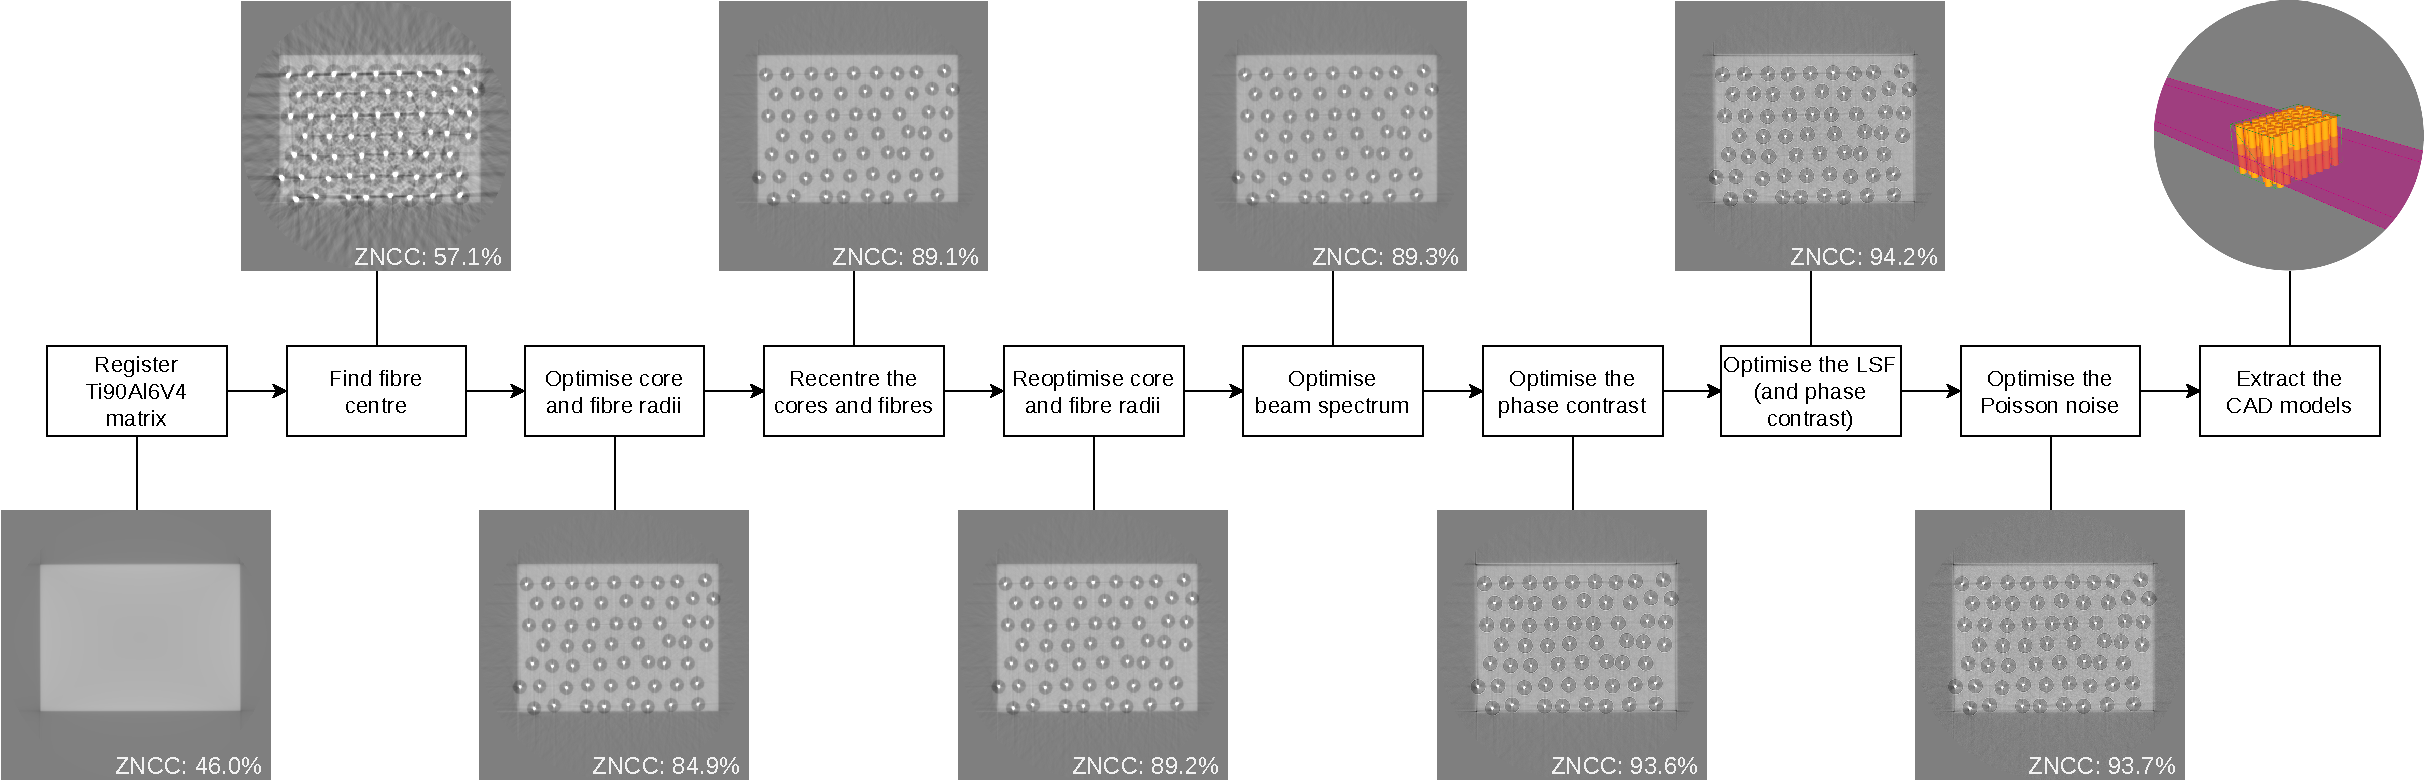
\includegraphics{../doc/pipeline.pdf}
\caption{Main steps of the registration pipeline.}
\end{figure}

\begin{enumerate}
\def\labelenumi{\arabic{enumi}.}
\tightlist
\item
  Initialisation

  \begin{itemize}
  \tightlist
  \item
    \hyperref[import-packages]{Import Python packages}
  \item
    \hyperref[global-variables]{Global variables} with values
    corresponding to known parameters
  \item
    \hyperref[load-the-image-data]{Load the image data from the experiment at ESRF}
  \item
    \hyperref[ct-reconstruction]{Recontruct the corresponding CT data}
  \item
    \hyperref[normalise-the-image-data]{Normalise the image data}
  \item
    \hyperref[set-the-x-ray-simulation-environment]{Set the X-ray simulation environment}
  \item
    \hyperref[the-lsf]{LSF}
  \item
    \hyperref[find-circles-to-identify-the-centre-of-fibres]{Find circles to identify the centre of fibres}
  \end{itemize}
\item
  \hyperref[simulate-the-ct-acquisition]{Simulate the CT acquisition}
\item
  \hyperref[registration-of-a-cube]{Registration of the Ti90Al6V4 matrix}
\item
  \hyperref[optimisation-of-the-cores-and-fibres-radii]{Optimisation of the cores and fibres radii}
\item
  \hyperref[recentre-each-corefibre]{Recentre each core/fibre}
\item
  \hyperref[optimisation-the-radii-after-recentring]{Optimisation the radii after recentring}
\item
  \hyperref[optimisation-of-the-beam-spectrum]{Optimisation of the beam spectrum}
\item
  \hyperref[optimisation-of-the-phase-contrast-and-the-radii]{Optimisation of the phase contrast and the radii}
\item
  \hyperref[optimisation-of-the-phase-contrast-and-the-lsf]{Optimisation of the phase contrast and the LSF}
\item
  \hyperref[optimisation-of-the-poisson-noise]{Optimisation of the Poisson noise}
\item
  \hyperref[results-in-terms-of-linear-attenuation-coefficients]{Results in terms of linear attenuation coefficients}
\end{enumerate}

    In image registration, a \emph{moving object} is geometrically deformed
so that its image matches a \emph{target image}. The parameters of the
deformation is controlled and iteratively tuned by an optimisation
algorithm.

\begin{figure}
\centering
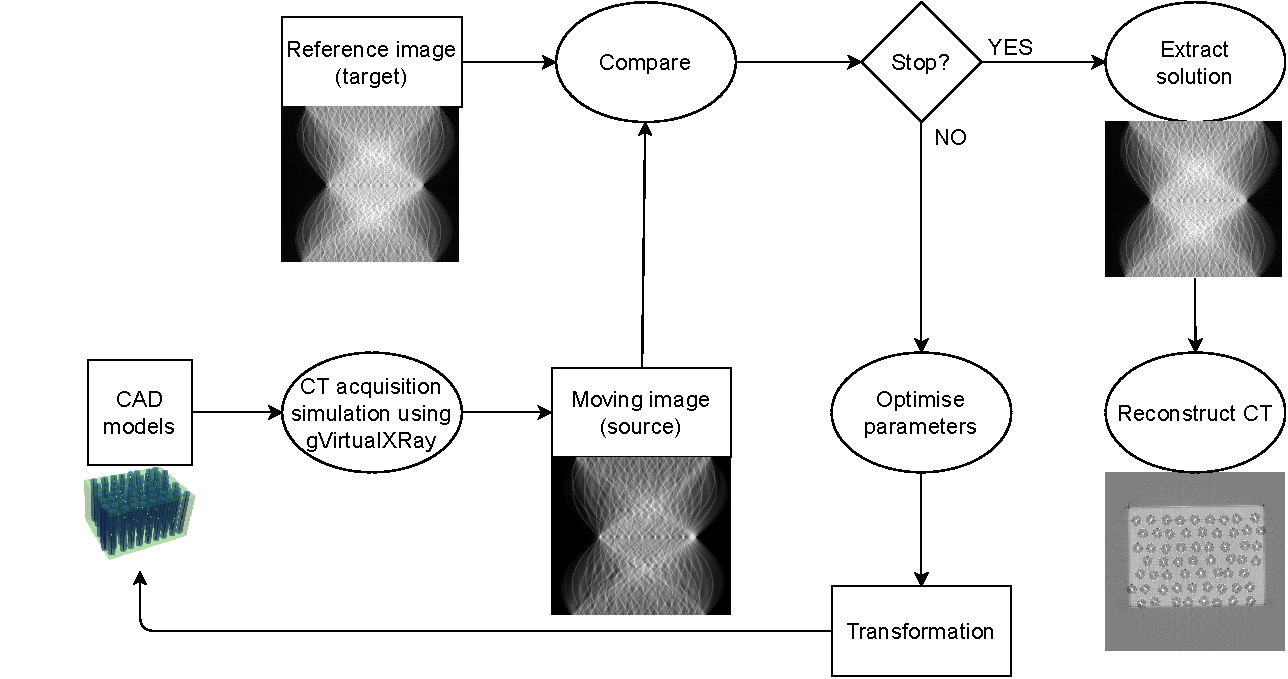
\includegraphics{../doc/registration.pdf}
\caption{Registration flowchart}
\end{figure}

In our context, the target is the sinogram provided by the experiment at
ESRF. The moving image is created by simulation using the CAD models and
\href{https://sourceforge.net/projects/gvirtualxray/}{gVirtualXRay}. The
simulation parameters controlling the CAD models are repetitively tuned
by a global optimisation algorithm until a stopping criterion is met.
The optimisation algorithm will minimise (or maximise) a numerical
value, the \emph{objective function}. The comparison between the target
and moving images measures how different (or similar) the two images
are. It is performed within the objective function.

    \hypertarget{import-packages}{%
\section{Import packages}\label{import-packages}}

We need to import a few libraries (called packages in Python). We use:

\begin{itemize}
\tightlist
\item
  \texttt{copy}: duplicating images using deepcopies;
\item
  \texttt{glob}: retrieving file names in a directory;
\item
  \texttt{math}: the \texttt{floor} function;
\item
  \texttt{os}: creating a new directory;
\item
  \texttt{sys}: retrieving the largest possible floating-point value;
\item
  \texttt{cma}: non-linear numerical optimization
  (\href{https://github.com/CMA-ES/pycma}{CMA-ES, Covariance Matrix
  Adaptation Evolution Strategy});
\item
  (\href{https://www.opencv.org/}{OpenCV}) (\texttt{cv2}): Hough
  transform and bilateral filter (an edge-preserving smoothing filter);
\item
  \texttt{imageio}: creating GIF files;
\item
  \texttt{IPython.display}: display Pandas'dataframes as HTML tables;
\item
  \texttt{matplotlib}: plotting data;
\item
  \texttt{mpl\_toolkits}: plotting 3D data (final CAD models);
\item
  \texttt{numpy}: who doesn't use numpy?
\item
  \texttt{pandas}: creating a DataFrame to store \(\mu\) data;
\item
  \href{https://simpleitk.org/}{SimpleITK}: image processing and saving
  volume data;
\item
  \texttt{tomopy}: package for CT reconstruction;
\item
  \texttt{scipy}: for the convolution of a 2D image by a 1D kernel;
\item
  \texttt{skimage}: comparing the reference CT slice and the simulated
  one;
\item
  \texttt{sklearn}: comparing the reference CT slice and the simulated
  one;
\item
  \texttt{stl}: to import STL files (CAD models);
\item
  \texttt{lsf}: the line spread function to filter the X-ray images; and
\item
  \texttt{gvxrPython3}:
  \href{http://gvirtualxray.sourceforge.net/}{gVirtualXRay}'s Python
  wrapper to simulate X-ray images using the Beer-Lambert law on GPU.
\end{itemize}

    \begin{tcolorbox}[breakable, size=fbox, boxrule=1pt, pad at break*=1mm,colback=cellbackground, colframe=cellborder]
\prompt{In}{incolor}{1}{\boxspacing}
\begin{Verbatim}[commandchars=\\\{\}]
\PY{o}{\PYZpc{}}\PY{k}{matplotlib} inline

\PY{k+kn}{import} \PY{n+nn}{copy}
\PY{k+kn}{import} \PY{n+nn}{glob}
\PY{k+kn}{import} \PY{n+nn}{math}
\PY{k+kn}{import} \PY{n+nn}{os}
\PY{k+kn}{import} \PY{n+nn}{sys}

\PY{k+kn}{import} \PY{n+nn}{cma}
\PY{k+kn}{import} \PY{n+nn}{cv2}
\PY{k+kn}{import} \PY{n+nn}{imageio}
\PY{k+kn}{import} \PY{n+nn}{matplotlib}\PY{n+nn}{.}\PY{n+nn}{pyplot} \PY{k}{as} \PY{n+nn}{plt}
\PY{k+kn}{import} \PY{n+nn}{numpy} \PY{k}{as} \PY{n+nn}{np}
\PY{k+kn}{import} \PY{n+nn}{pandas} \PY{k}{as} \PY{n+nn}{pd}
\PY{k+kn}{import} \PY{n+nn}{SimpleITK} \PY{k}{as} \PY{n+nn}{sitk}
\PY{k+kn}{import} \PY{n+nn}{tomopy}

\PY{k+kn}{from} \PY{n+nn}{IPython}\PY{n+nn}{.}\PY{n+nn}{display} \PY{k+kn}{import} \PY{n}{display}
\PY{k+kn}{from} \PY{n+nn}{matplotlib} \PY{k+kn}{import} \PY{n}{cm}
\PY{k+kn}{from} \PY{n+nn}{mpl\PYZus{}toolkits} \PY{k+kn}{import} \PY{n}{mplot3d}
\PY{k+kn}{from} \PY{n+nn}{scipy} \PY{k+kn}{import} \PY{n}{ndimage}
\PY{k+kn}{from} \PY{n+nn}{skimage}\PY{n+nn}{.}\PY{n+nn}{metrics} \PY{k+kn}{import} \PY{n}{structural\PYZus{}similarity} \PY{k}{as} \PY{n}{ssim}
\PY{k+kn}{from} \PY{n+nn}{skimage}\PY{n+nn}{.}\PY{n+nn}{util} \PY{k+kn}{import} \PY{n}{compare\PYZus{}images}
\PY{k+kn}{from} \PY{n+nn}{sklearn}\PY{n+nn}{.}\PY{n+nn}{metrics} \PY{k+kn}{import} \PY{n}{mean\PYZus{}absolute\PYZus{}error}\PY{p}{,} \PY{n}{mean\PYZus{}squared\PYZus{}error}
\PY{k+kn}{from} \PY{n+nn}{stl} \PY{k+kn}{import} \PY{n}{mesh}

\PY{n}{plt}\PY{o}{.}\PY{n}{ioff}\PY{p}{(}\PY{p}{)}
\PY{n}{plt}\PY{o}{.}\PY{n}{rcParams}\PY{p}{[}\PY{l+s+s1}{\PYZsq{}}\PY{l+s+s1}{figure.figsize}\PY{l+s+s1}{\PYZsq{}}\PY{p}{]} \PY{o}{=} \PY{p}{[}\PY{l+m+mi}{12}\PY{p}{,} \PY{l+m+mi}{8}\PY{p}{]}
\PY{n}{plt}\PY{o}{.}\PY{n}{rcParams}\PY{p}{[}\PY{l+s+s1}{\PYZsq{}}\PY{l+s+s1}{figure.dpi}\PY{l+s+s1}{\PYZsq{}}\PY{p}{]} \PY{o}{=} \PY{l+m+mi}{100} \PY{c+c1}{\PYZsh{} 200 e.g. is really fine, but slower}

\PY{k+kn}{import} \PY{n+nn}{gvxrPython3} \PY{k}{as} \PY{n+nn}{gvxr}

\PY{k+kn}{from} \PY{n+nn}{lsf} \PY{k+kn}{import} \PY{o}{*}
\end{Verbatim}
\end{tcolorbox}

    \begin{tcolorbox}[breakable, size=fbox, boxrule=1pt, pad at break*=1mm,colback=cellbackground, colframe=cellborder]
\prompt{In}{incolor}{2}{\boxspacing}
\begin{Verbatim}[commandchars=\\\{\}]
\PY{k}{if} \PY{o+ow}{not} \PY{n}{os}\PY{o}{.}\PY{n}{path}\PY{o}{.}\PY{n}{exists}\PY{p}{(}\PY{l+s+s2}{\PYZdq{}}\PY{l+s+s2}{outputs}\PY{l+s+s2}{\PYZdq{}}\PY{p}{)}\PY{p}{:}
    \PY{n}{os}\PY{o}{.}\PY{n}{makedirs}\PY{p}{(}\PY{l+s+s2}{\PYZdq{}}\PY{l+s+s2}{outputs}\PY{l+s+s2}{\PYZdq{}}\PY{p}{)}\PY{p}{;}

\PY{k}{if} \PY{o+ow}{not} \PY{n}{os}\PY{o}{.}\PY{n}{path}\PY{o}{.}\PY{n}{exists}\PY{p}{(}\PY{l+s+s2}{\PYZdq{}}\PY{l+s+s2}{plots}\PY{l+s+s2}{\PYZdq{}}\PY{p}{)}\PY{p}{:}
    \PY{n}{os}\PY{o}{.}\PY{n}{makedirs}\PY{p}{(}\PY{l+s+s2}{\PYZdq{}}\PY{l+s+s2}{plots}\PY{l+s+s2}{\PYZdq{}}\PY{p}{)}\PY{p}{;}
\end{Verbatim}
\end{tcolorbox}

    \hypertarget{global-variables}{%
\section{Global variables}\label{global-variables}}

We need some global variables:

\begin{itemize}
\tightlist
\item
  \texttt{NoneType}: the type of \texttt{None};
\item
  \texttt{pixel\_spacing\_in\_micrometre}: the physical distance between
  the centre of two successive pixel;
\item
  \texttt{pixel\_spacing\_in\_mm}: the physical distance between the
  centre of two successive pixel;
\item
  \texttt{number\_of\_projections}: the total number of angles in the
  sinogram;he total number of angles in the sinogram;
\item
  \texttt{angular\_span\_in\_degrees}: the angular span covered by the
  sinogram;
\item
  \texttt{angular\_step}: the angular step;
\item
  \texttt{theta}: the rotation angles in degrees (vertical axis of the
  sinogram);
\item
  \texttt{theta\_rad}: the rotation angles in radians (vertical axis of
  the sinogram);
\item
  \texttt{roi\_length}: control the size of the ROI when displayng the
  central fibre;
\item
  \texttt{value\_range}: control the binning of the Laplacian kernel
\item
  \texttt{num\_samples}: control the binning of the Laplacian kernel
\item
  \texttt{sigma\_set}: spread of the Laplacian kernels
\item
  \texttt{k\_set}: weight of the Laplacian kernels
\item
  \texttt{label\_set}: label of the structures on which a Laplacian
  kernel is applied
\item
  \texttt{bias}: control the bias of the Poisson noise
\item
  \texttt{gain}: control the gain of the Poisson noise: control the bias
  of the Poisson noise
\item
  \texttt{scale}: control the scale of the Poisson noise: control the
  bias of the Poisson noise
\item
  \texttt{use\_normalisation}: use or do not use zero-mean,
  unit-variance normalisation in the objective functions;
\item
  \texttt{use\_sinogram}: compute the objective functions on the
  sinogram or flat-field;
\item
  \texttt{metrics\_type}: type of image comparison used in the objective
  functions;
\item
  \texttt{fibre\_radius}: radius of the SiC fibres in um
\item
  \texttt{core\_radius}: radius of the W fibres in um
\end{itemize}

    \begin{tcolorbox}[breakable, size=fbox, boxrule=1pt, pad at break*=1mm,colback=cellbackground, colframe=cellborder]
\prompt{In}{incolor}{3}{\boxspacing}
\begin{Verbatim}[commandchars=\\\{\}]
\PY{n}{NoneType} \PY{o}{=} \PY{n+nb}{type}\PY{p}{(}\PY{k+kc}{None}\PY{p}{)}\PY{p}{;}
\PY{n}{pixel\PYZus{}spacing\PYZus{}in\PYZus{}micrometre} \PY{o}{=} \PY{l+m+mf}{1.9}\PY{p}{;}
\PY{n}{pixel\PYZus{}spacing\PYZus{}in\PYZus{}mm} \PY{o}{=} \PY{n}{pixel\PYZus{}spacing\PYZus{}in\PYZus{}micrometre} \PY{o}{*} \PY{l+m+mf}{1e\PYZhy{}3}\PY{p}{;}
\PY{n}{number\PYZus{}of\PYZus{}projections} \PY{o}{=} \PY{l+m+mi}{900}\PY{p}{;}
\PY{n}{angular\PYZus{}span\PYZus{}in\PYZus{}degrees} \PY{o}{=} \PY{l+m+mf}{180.0}\PY{p}{;}
\PY{n}{angular\PYZus{}step} \PY{o}{=} \PY{n}{angular\PYZus{}span\PYZus{}in\PYZus{}degrees} \PY{o}{/} \PY{n}{number\PYZus{}of\PYZus{}projections}\PY{p}{;}
\PY{n}{theta} \PY{o}{=} \PY{n}{np}\PY{o}{.}\PY{n}{linspace}\PY{p}{(}\PY{l+m+mf}{0.}\PY{p}{,}
                    \PY{n}{angular\PYZus{}span\PYZus{}in\PYZus{}degrees}\PY{p}{,}
                    \PY{n}{number\PYZus{}of\PYZus{}projections}\PY{p}{,}
                    \PY{n}{endpoint}\PY{o}{=}\PY{k+kc}{False}\PY{p}{)}\PY{p}{;}
\PY{n}{theta\PYZus{}rad} \PY{o}{=} \PY{n}{theta} \PY{o}{/} \PY{l+m+mf}{180.0} \PY{o}{*} \PY{n}{math}\PY{o}{.}\PY{n}{pi}\PY{p}{;}

\PY{n}{roi\PYZus{}length} \PY{o}{=} \PY{l+m+mi}{60}\PY{p}{;}

\PY{n}{value\PYZus{}range} \PY{o}{=} \PY{l+m+mi}{6}\PY{p}{;}
\PY{n}{num\PYZus{}samples} \PY{o}{=} \PY{l+m+mi}{15}\PY{p}{;}

\PY{n}{sigma\PYZus{}set} \PY{o}{=} \PY{k+kc}{None}\PY{p}{;}
\PY{n}{k\PYZus{}set} \PY{o}{=} \PY{k+kc}{None}\PY{p}{;}
\PY{n}{label\PYZus{}set} \PY{o}{=} \PY{k+kc}{None}\PY{p}{;}

\PY{n}{bias} \PY{o}{=} \PY{k+kc}{None}\PY{p}{;}
\PY{n}{gain} \PY{o}{=} \PY{k+kc}{None}\PY{p}{;}
\PY{n}{scale} \PY{o}{=} \PY{k+kc}{None}\PY{p}{;}

\PY{n}{use\PYZus{}normalisation} \PY{o}{=} \PY{k+kc}{True}\PY{p}{;}
\PY{n}{use\PYZus{}sinogram} \PY{o}{=} \PY{k+kc}{True}\PY{p}{;}

\PY{n}{metrics\PYZus{}type} \PY{o}{=} \PY{l+s+s2}{\PYZdq{}}\PY{l+s+s2}{RMSE}\PY{l+s+s2}{\PYZdq{}}\PY{p}{;}

\PY{n}{fibre\PYZus{}radius} \PY{o}{=} \PY{l+m+mi}{140} \PY{o}{/} \PY{l+m+mi}{2}\PY{p}{;}  \PY{c+c1}{\PYZsh{} um}
\PY{n}{core\PYZus{}radius} \PY{o}{=} \PY{l+m+mi}{30} \PY{o}{/} \PY{l+m+mi}{2}\PY{p}{;}  \PY{c+c1}{\PYZsh{} um}
\end{Verbatim}
\end{tcolorbox}

    \hypertarget{load-the-image-data}{%
\section{Load the image data}\label{load-the-image-data}}

Load and display the reference projections from a raw binary file,
i.e.~the target of the registration.

    \begin{tcolorbox}[breakable, size=fbox, boxrule=1pt, pad at break*=1mm,colback=cellbackground, colframe=cellborder]
\prompt{In}{incolor}{4}{\boxspacing}
\begin{Verbatim}[commandchars=\\\{\}]
\PY{c+c1}{\PYZsh{} Target of the registration}
\PY{n}{reference\PYZus{}normalised\PYZus{}projections} \PY{o}{=} \PY{n}{np}\PY{o}{.}\PY{n}{fromfile}\PY{p}{(}\PY{l+s+s2}{\PYZdq{}}\PY{l+s+s2}{sino.raw}\PY{l+s+s2}{\PYZdq{}}\PY{p}{,} \PY{n}{dtype}\PY{o}{=}\PY{n}{np}\PY{o}{.}\PY{n}{float32}\PY{p}{)}\PY{p}{;}
\PY{n}{reference\PYZus{}normalised\PYZus{}projections}\PY{o}{.}\PY{n}{shape} \PY{o}{=} \PY{p}{[}
    \PY{n}{number\PYZus{}of\PYZus{}projections}\PY{p}{,}
    \PY{n+nb}{int}\PY{p}{(}\PY{n}{reference\PYZus{}normalised\PYZus{}projections}\PY{o}{.}\PY{n}{shape}\PY{p}{[}\PY{l+m+mi}{0}\PY{p}{]} \PY{o}{/} \PY{n}{number\PYZus{}of\PYZus{}projections}\PY{p}{)}
\PY{p}{]}\PY{p}{;}
\end{Verbatim}
\end{tcolorbox}

    We define a function to save raw images in the MHA format:

    \begin{tcolorbox}[breakable, size=fbox, boxrule=1pt, pad at break*=1mm,colback=cellbackground, colframe=cellborder]
\prompt{In}{incolor}{5}{\boxspacing}
\begin{Verbatim}[commandchars=\\\{\}]
\PY{k}{def} \PY{n+nf}{saveMHA}\PY{p}{(}\PY{n}{fname}\PY{p}{,} \PY{n}{image}\PY{p}{,} \PY{n}{spacing}\PY{p}{)}\PY{p}{:}
    \PY{l+s+sd}{\PYZdq{}\PYZdq{}\PYZdq{}}
\PY{l+s+sd}{    save the image into a file.}

\PY{l+s+sd}{    :param str fname: the filename}
\PY{l+s+sd}{    :param 2D\PYZus{}image image: the image to save}
\PY{l+s+sd}{    :param [flt, flt, flt] spacing: the space between two successive voxels along the 3 direction}
\PY{l+s+sd}{    \PYZdq{}\PYZdq{}\PYZdq{}}

    \PY{n}{volume} \PY{o}{=} \PY{n}{sitk}\PY{o}{.}\PY{n}{GetImageFromArray}\PY{p}{(}\PY{n}{image}\PY{p}{)}\PY{p}{;}
    \PY{n}{volume}\PY{o}{.}\PY{n}{SetSpacing}\PY{p}{(}\PY{n}{spacing}\PY{p}{)}\PY{p}{;}
    \PY{n}{sitk}\PY{o}{.}\PY{n}{WriteImage}\PY{p}{(}\PY{n}{volume}\PY{p}{,} \PY{n}{fname}\PY{p}{,} \PY{n}{useCompression}\PY{o}{=}\PY{k+kc}{True}\PY{p}{)}\PY{p}{;}
\end{Verbatim}
\end{tcolorbox}

    The reference projections in a MHA file

    \begin{tcolorbox}[breakable, size=fbox, boxrule=1pt, pad at break*=1mm,colback=cellbackground, colframe=cellborder]
\prompt{In}{incolor}{6}{\boxspacing}
\begin{Verbatim}[commandchars=\\\{\}]
\PY{n}{saveMHA}\PY{p}{(}\PY{l+s+s1}{\PYZsq{}}\PY{l+s+s1}{outputs/reference\PYZus{}normalised\PYZus{}projections.mha}\PY{l+s+s1}{\PYZsq{}}\PY{p}{,} \PY{n}{reference\PYZus{}normalised\PYZus{}projections}\PY{p}{,} \PY{p}{[}\PY{n}{pixel\PYZus{}spacing\PYZus{}in\PYZus{}mm}\PY{p}{,} \PY{n}{angular\PYZus{}step}\PY{p}{,} \PY{n}{pixel\PYZus{}spacing\PYZus{}in\PYZus{}mm}\PY{p}{]}\PY{p}{)}\PY{p}{;}
\end{Verbatim}
\end{tcolorbox}

    Display the reference projections using Matplotlib

    \begin{tcolorbox}[breakable, size=fbox, boxrule=1pt, pad at break*=1mm,colback=cellbackground, colframe=cellborder]
\prompt{In}{incolor}{7}{\boxspacing}
\begin{Verbatim}[commandchars=\\\{\}]
\PY{n}{labels} \PY{o}{=} \PY{p}{[}\PY{n}{theta}\PY{p}{[}\PY{l+m+mi}{0}\PY{p}{]}\PY{p}{,} \PY{n}{theta}\PY{p}{[}\PY{n}{reference\PYZus{}normalised\PYZus{}projections}\PY{o}{.}\PY{n}{shape}\PY{p}{[}\PY{l+m+mi}{0}\PY{p}{]} \PY{o}{/}\PY{o}{/} \PY{l+m+mi}{2}\PY{p}{]}\PY{p}{,} \PY{n}{theta}\PY{p}{[}\PY{o}{\PYZhy{}}\PY{l+m+mi}{1}\PY{p}{]}\PY{p}{]}\PY{p}{;}
\PY{n}{tics} \PY{o}{=} \PY{p}{[}
    \PY{l+m+mi}{0}\PY{p}{,}
    \PY{n}{reference\PYZus{}normalised\PYZus{}projections}\PY{o}{.}\PY{n}{shape}\PY{p}{[}\PY{l+m+mi}{0}\PY{p}{]} \PY{o}{/}\PY{o}{/} \PY{l+m+mi}{2}\PY{p}{,}
    \PY{n}{reference\PYZus{}normalised\PYZus{}projections}\PY{o}{.}\PY{n}{shape}\PY{p}{[}\PY{l+m+mi}{0}\PY{p}{]}\PY{o}{\PYZhy{}}\PY{l+m+mi}{1}
\PY{p}{]}\PY{p}{;}
\PY{n}{fig} \PY{o}{=} \PY{n}{plt}\PY{o}{.}\PY{n}{figure}\PY{p}{(}\PY{p}{)}\PY{p}{;}
\PY{n}{imgplot} \PY{o}{=} \PY{n}{plt}\PY{o}{.}\PY{n}{imshow}\PY{p}{(}\PY{n}{reference\PYZus{}normalised\PYZus{}projections}\PY{p}{,} \PY{n}{cmap}\PY{o}{=}\PY{l+s+s2}{\PYZdq{}}\PY{l+s+s2}{gray}\PY{l+s+s2}{\PYZdq{}}\PY{p}{)}\PY{p}{;}
\PY{n}{plt}\PY{o}{.}\PY{n}{xlabel}\PY{p}{(}\PY{l+s+s2}{\PYZdq{}}\PY{l+s+s2}{Displacement of projection}\PY{l+s+s2}{\PYZdq{}}\PY{p}{)}\PY{p}{;}
\PY{n}{plt}\PY{o}{.}\PY{n}{ylabel}\PY{p}{(}\PY{l+s+s2}{\PYZdq{}}\PY{l+s+s2}{Angle of projection (in degrees)}\PY{l+s+s2}{\PYZdq{}}\PY{p}{)}\PY{p}{;}
\PY{n}{plt}\PY{o}{.}\PY{n}{yticks}\PY{p}{(}\PY{n}{tics}\PY{p}{,} \PY{n}{labels}\PY{p}{)}\PY{p}{;}
\PY{n}{plt}\PY{o}{.}\PY{n}{title}\PY{p}{(}\PY{l+s+s2}{\PYZdq{}}\PY{l+s+s2}{Projections after flat\PYZhy{}field correction from the experiment at ESRF}\PY{l+s+s2}{\PYZdq{}}\PY{p}{)}\PY{p}{;}
\PY{n}{fig}\PY{o}{.}\PY{n}{colorbar}\PY{p}{(}\PY{n}{imgplot}\PY{p}{)}\PY{p}{;}
\PY{n}{plt}\PY{o}{.}\PY{n}{savefig}\PY{p}{(}\PY{l+s+s1}{\PYZsq{}}\PY{l+s+s1}{plots/Normalised\PYZus{}projections\PYZus{}from\PYZus{}experiment\PYZus{}ESRF.pdf}\PY{l+s+s1}{\PYZsq{}}\PY{p}{)}
\PY{n}{plt}\PY{o}{.}\PY{n}{savefig}\PY{p}{(}\PY{l+s+s1}{\PYZsq{}}\PY{l+s+s1}{plots/Normalised\PYZus{}projections\PYZus{}from\PYZus{}experiment\PYZus{}ESRF.png}\PY{l+s+s1}{\PYZsq{}}\PY{p}{)}
\end{Verbatim}
\end{tcolorbox}

    In the literature, a projection is often modelled using the
polychromatic version of the Beer-Lambert law:
\[\mathbf{I}(x,y) = \sum_i \mathbf{R}_i \, \mathbf{N}_i \; \exp\left({-\sum_j \mu_j(E_i) \; \mathbf{d}_j(x,y)}\right)\]

\begin{itemize}
\tightlist
\item
  \(\mathbf{I}(x,y)\) the value of the raw X-ray projection at pixel
  location \((x,y)\), and with the sample and with the X-ray beam turned
  on;
\item
  \(i\) the \(i\)-th energy channel in the beam spectrum;\\
\item
  \(E_i\) the energy in eV;
\item
  \(\mathbf{R}_i\) and \(\mathbf{N}_i\) the detector response and the
  number of photons at that energy respectively;
\item
  \(j\) the \(j\)-th material being scanned, \(\mu_j(E_i)\) its linear
  attenuation coefficient at energy \(E_i\), and
\item
  \(\mathbf{d}_j(x,y)\) path length in cm\(^{-1}\) of the ray crossing
  the \(j\)-th material from the X-ray source to pixel \((x,y)\).
\end{itemize}

Projections are then corrected to account for variations in beam
homogeneity and in the pixel-to-pixel sensitivity of the detector. This
is the projection with flat-field correction (\(\mathbf{Proj}\)):
\[\mathbf{Proj} = \frac{\mathbf{I} - \mathbf{D}}{\mathbf{F} - \mathbf{D}}\]
\(\mathbf{F}\) (full fields) and \(\mathbf{D}\) (dark fields) are
projection images without sample and acquired with and without the X-ray
beam turned on respectively. Note that with an ideal detector
(\(\mathbf{R}_i=E_i\)), pixels of \(\mathbf{D}\) are null, and pixels of
\(\mathbf{F}\) are equal to \(\sum_i E_i \; \mathbf{N}_i\).

\begin{figure}
\centering
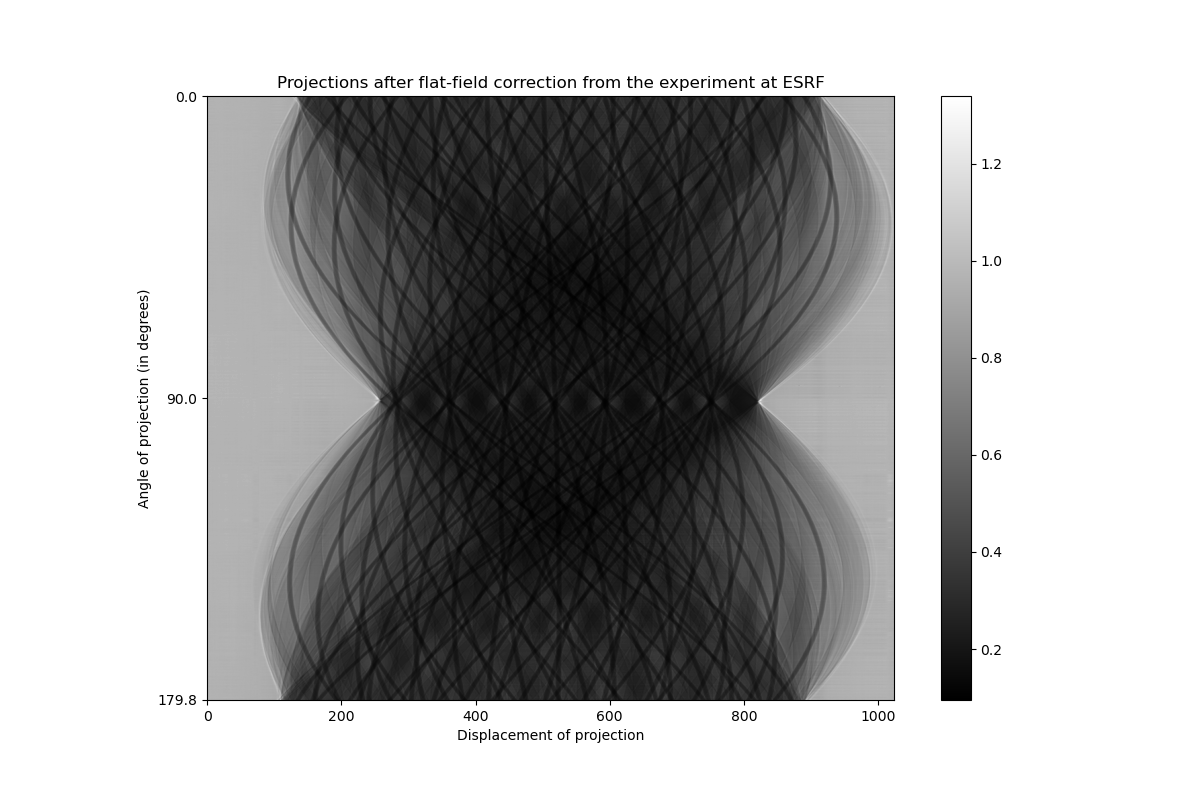
\includegraphics{plots/Normalised_projections_from_experiment_ESRF.png}
\caption{Projections after flat-field correction from the experiment at
ESRF}
\end{figure}

\texttt{reference\_normalised\_projections} (the figure above)
corresponds to the data loaded from the binary file. It corresponds to
\(\mathbf{Proj}\), i.e.~the flat-field correction has already been
performed.

We can see that when the primary spectrum is not monochromatic the
measurement is the sum of several attenuation laws. We could however
compute the effective monochromatic attenuation that would give the same
measurement:
\[    \mathbf{I}(x,y) = \mathbf{I}_0(x,y) \; \exp\left({-\sum_j \mu_j(E_{\mathrm{eff}}) \; \mathbf{d}_j(x,y)}\right)\]

with \(\mathbf{I}_0(x,y) = \sum_i \mathbf{R}_i \, \mathbf{N}_i\), and
where \(E_{\mathrm{eff}}\) corresponds to the monochromatic energy that
would give the same attenuation than the one measured. We are now able
to linearise the transmission tomography data, namely \(\mathbf{Proj}\),
and we get the sinogram:
\[\textbf{Sino}=-\ln\left(\textbf{Proj}\right)\]

We define a new function to compute the sinogram from flat-field
correction and calls it straightaway.

    \begin{tcolorbox}[breakable, size=fbox, boxrule=1pt, pad at break*=1mm,colback=cellbackground, colframe=cellborder]
\prompt{In}{incolor}{8}{\boxspacing}
\begin{Verbatim}[commandchars=\\\{\}]
\PY{k}{def} \PY{n+nf}{computeSinogramFromFlatField}\PY{p}{(}\PY{n}{normalised\PYZus{}projections}\PY{p}{)}\PY{p}{:}
    \PY{l+s+sd}{\PYZdq{}\PYZdq{}\PYZdq{}}
\PY{l+s+sd}{    This function apply the minus log normalisation}
\PY{l+s+sd}{    on the projections that bave been corrected with the flat\PYZhy{}field method.}

\PY{l+s+sd}{    :param 2D\PYZus{}image normalised\PYZus{}projections: The projections after flat\PYZhy{}field corrections}
\PY{l+s+sd}{    :return the sinogram.}
\PY{l+s+sd}{    \PYZdq{}\PYZdq{}\PYZdq{}}

    \PY{c+c1}{\PYZsh{} Create a temporary image to hold the sinogram}
    \PY{n}{simulated\PYZus{}sinogram} \PY{o}{=} \PY{n}{copy}\PY{o}{.}\PY{n}{deepcopy}\PY{p}{(}\PY{n}{normalised\PYZus{}projections}\PY{p}{)}\PY{p}{;}

    \PY{c+c1}{\PYZsh{} Make sure no value is negative or null (because of the log function)}
    \PY{c+c1}{\PYZsh{} It should not be the case, however, when the Laplacian is used to simulate}
    \PY{c+c1}{\PYZsh{} phase contrast, negative values can be generated.}
    \PY{n}{threshold} \PY{o}{=} \PY{l+m+mf}{0.000001}
    \PY{n}{simulated\PYZus{}sinogram}\PY{p}{[}\PY{n}{simulated\PYZus{}sinogram} \PY{o}{\PYZlt{}} \PY{n}{threshold}\PY{p}{]} \PY{o}{=} \PY{n}{threshold}\PY{p}{;}

    \PY{c+c1}{\PYZsh{} Apply the minus log normalisation}
    \PY{n}{simulated\PYZus{}sinogram} \PY{o}{=} \PY{o}{\PYZhy{}}\PY{n}{np}\PY{o}{.}\PY{n}{log}\PY{p}{(}\PY{n}{simulated\PYZus{}sinogram}\PY{p}{)}\PY{p}{;}

    \PY{c+c1}{\PYZsh{} Rescale the data taking into account the pixel size}
    \PY{n}{simulated\PYZus{}sinogram} \PY{o}{/}\PY{o}{=} \PY{n}{pixel\PYZus{}spacing\PYZus{}in\PYZus{}micrometre} \PY{o}{*} \PY{n}{gvxr}\PY{o}{.}\PY{n}{getUnitOfLength}\PY{p}{(}\PY{l+s+s2}{\PYZdq{}}\PY{l+s+s2}{um}\PY{l+s+s2}{\PYZdq{}}\PY{p}{)} \PY{o}{/} \PY{n}{gvxr}\PY{o}{.}\PY{n}{getUnitOfLength}\PY{p}{(}\PY{l+s+s2}{\PYZdq{}}\PY{l+s+s2}{cm}\PY{l+s+s2}{\PYZdq{}}\PY{p}{)}\PY{p}{;}

    \PY{c+c1}{\PYZsh{} Return the new image}
    \PY{k}{return} \PY{n}{simulated\PYZus{}sinogram}\PY{p}{;}
\end{Verbatim}
\end{tcolorbox}

    Compute the sinogram from the flat-field data

    \begin{tcolorbox}[breakable, size=fbox, boxrule=1pt, pad at break*=1mm,colback=cellbackground, colframe=cellborder]
\prompt{In}{incolor}{9}{\boxspacing}
\begin{Verbatim}[commandchars=\\\{\}]
\PY{n}{reference\PYZus{}sinogram} \PY{o}{=} \PY{n}{computeSinogramFromFlatField}\PY{p}{(}\PY{n}{reference\PYZus{}normalised\PYZus{}projections}\PY{p}{)}\PY{p}{;}
\end{Verbatim}
\end{tcolorbox}

    Save the corresponding image

    \begin{tcolorbox}[breakable, size=fbox, boxrule=1pt, pad at break*=1mm,colback=cellbackground, colframe=cellborder]
\prompt{In}{incolor}{10}{\boxspacing}
\begin{Verbatim}[commandchars=\\\{\}]
\PY{n}{saveMHA}\PY{p}{(}\PY{l+s+s1}{\PYZsq{}}\PY{l+s+s1}{outputs/reference\PYZus{}sinogram.mha}\PY{l+s+s1}{\PYZsq{}}\PY{p}{,} \PY{n}{reference\PYZus{}sinogram}\PY{p}{,} \PY{p}{[}\PY{n}{pixel\PYZus{}spacing\PYZus{}in\PYZus{}mm}\PY{p}{,} \PY{n}{angular\PYZus{}step}\PY{p}{,} \PY{n}{pixel\PYZus{}spacing\PYZus{}in\PYZus{}mm}\PY{p}{]}\PY{p}{)}\PY{p}{;}
\end{Verbatim}
\end{tcolorbox}

    Display the sinogram using Matplotlib

    \begin{tcolorbox}[breakable, size=fbox, boxrule=1pt, pad at break*=1mm,colback=cellbackground, colframe=cellborder]
\prompt{In}{incolor}{11}{\boxspacing}
\begin{Verbatim}[commandchars=\\\{\}]
\PY{n}{labels}\PY{o}{=}\PY{p}{[}\PY{n}{theta}\PY{p}{[}\PY{l+m+mi}{0}\PY{p}{]}\PY{p}{,} \PY{n}{theta}\PY{p}{[}\PY{n}{reference\PYZus{}sinogram}\PY{o}{.}\PY{n}{shape}\PY{p}{[}\PY{l+m+mi}{0}\PY{p}{]} \PY{o}{/}\PY{o}{/} \PY{l+m+mi}{2}\PY{p}{]}\PY{p}{,} \PY{n}{theta}\PY{p}{[}\PY{o}{\PYZhy{}}\PY{l+m+mi}{1}\PY{p}{]}\PY{p}{]}\PY{p}{;}
\PY{n}{tics}\PY{o}{=}\PY{p}{[}\PY{l+m+mi}{0}\PY{p}{,} \PY{n}{reference\PYZus{}sinogram}\PY{o}{.}\PY{n}{shape}\PY{p}{[}\PY{l+m+mi}{0}\PY{p}{]} \PY{o}{/}\PY{o}{/} \PY{l+m+mi}{2}\PY{p}{,} \PY{n}{reference\PYZus{}sinogram}\PY{o}{.}\PY{n}{shape}\PY{p}{[}\PY{l+m+mi}{0}\PY{p}{]}\PY{o}{\PYZhy{}}\PY{l+m+mi}{1}\PY{p}{]}\PY{p}{;}
\PY{n}{fig}\PY{o}{=}\PY{n}{plt}\PY{o}{.}\PY{n}{figure}\PY{p}{(}\PY{p}{)}\PY{p}{;}
\PY{n}{imgplot} \PY{o}{=} \PY{n}{plt}\PY{o}{.}\PY{n}{imshow}\PY{p}{(}\PY{n}{reference\PYZus{}sinogram}\PY{p}{,} \PY{n}{cmap}\PY{o}{=}\PY{l+s+s2}{\PYZdq{}}\PY{l+s+s2}{gray}\PY{l+s+s2}{\PYZdq{}}\PY{p}{)}\PY{p}{;}
\PY{n}{plt}\PY{o}{.}\PY{n}{xlabel}\PY{p}{(}\PY{l+s+s2}{\PYZdq{}}\PY{l+s+s2}{Displacement of projection}\PY{l+s+s2}{\PYZdq{}}\PY{p}{)}\PY{p}{;}
\PY{n}{plt}\PY{o}{.}\PY{n}{ylabel}\PY{p}{(}\PY{l+s+s2}{\PYZdq{}}\PY{l+s+s2}{Angle of projection (in degrees)}\PY{l+s+s2}{\PYZdq{}}\PY{p}{)}\PY{p}{;}
\PY{n}{plt}\PY{o}{.}\PY{n}{yticks}\PY{p}{(}\PY{n}{tics}\PY{p}{,} \PY{n}{labels}\PY{p}{)}\PY{p}{;}
\PY{n}{plt}\PY{o}{.}\PY{n}{title}\PY{p}{(}\PY{l+s+s2}{\PYZdq{}}\PY{l+s+s2}{Sinogram of the reference image}\PY{l+s+s2}{\PYZdq{}}\PY{p}{)}\PY{p}{;}
\PY{n}{fig}\PY{o}{.}\PY{n}{colorbar}\PY{p}{(}\PY{n}{imgplot}\PY{p}{)}\PY{p}{;}
\PY{n}{plt}\PY{o}{.}\PY{n}{savefig}\PY{p}{(}\PY{l+s+s1}{\PYZsq{}}\PY{l+s+s1}{plots/Sinogram\PYZus{}reference\PYZus{}image.pdf}\PY{l+s+s1}{\PYZsq{}}\PY{p}{)}\PY{p}{;}
\PY{n}{plt}\PY{o}{.}\PY{n}{savefig}\PY{p}{(}\PY{l+s+s1}{\PYZsq{}}\PY{l+s+s1}{plots/Sinogram\PYZus{}reference\PYZus{}image.png}\PY{l+s+s1}{\PYZsq{}}\PY{p}{)}\PY{p}{;}
\end{Verbatim}
\end{tcolorbox}

    \begin{figure}
\centering
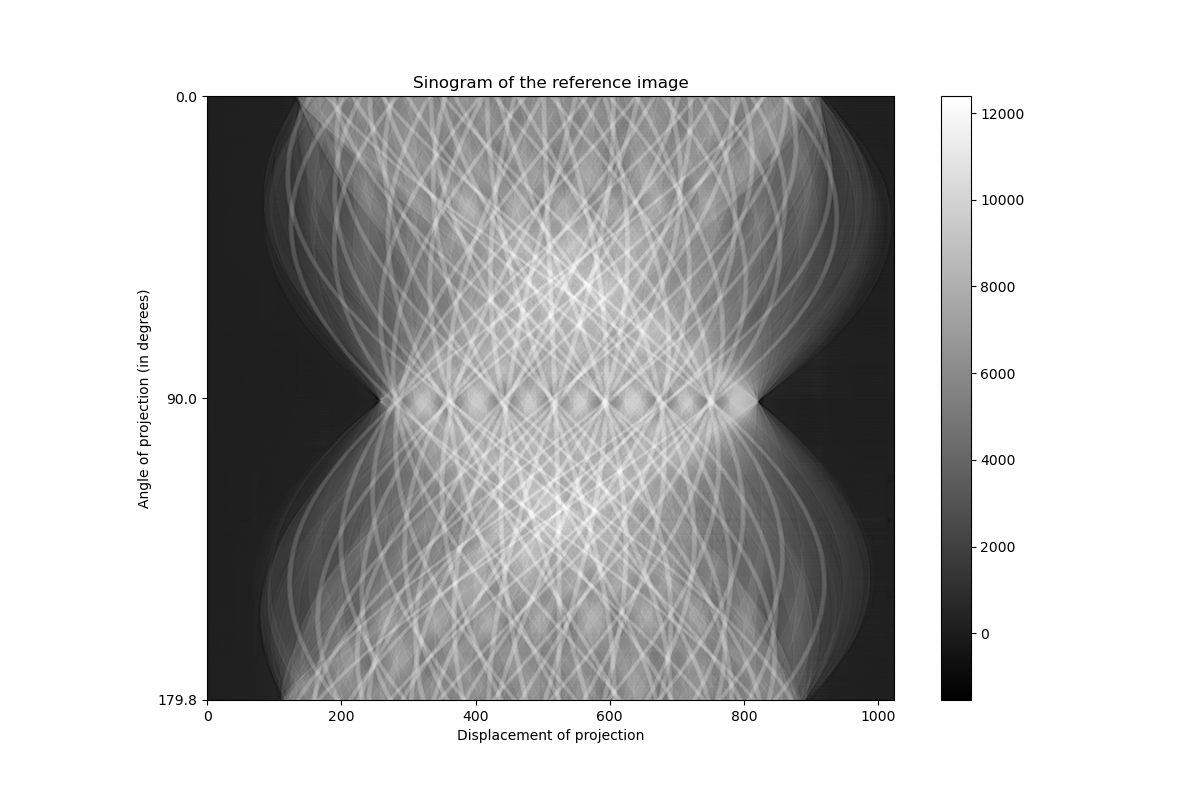
\includegraphics{plots/Sinogram_reference_image.png}
\caption{Sinogram of the reference image}
\end{figure}

\hypertarget{ct-reconstruction}{%
\section{CT reconstruction}\label{ct-reconstruction}}

Now we got a sinogram, we can reconstruct the CT slice. As we used a
synchrotron, we can assume we have a parallel source. It means we can
use a FBP rather than the FDK algorithm. In fact we use the gridrec
algorithm, which is much faster:

Dowd BA, Campbell GH, Marr RB, Nagarkar VV, Tipnis SV, Axe L, and
Siddons DP. \href{https://doi.org/10.1117/12.363725}{Developments in
synchrotron x-ray computed microtomography at the national synchrotron
light source}. In Proc. SPIE, volume 3772, 224--236. 1999.

    \begin{tcolorbox}[breakable, size=fbox, boxrule=1pt, pad at break*=1mm,colback=cellbackground, colframe=cellborder]
\prompt{In}{incolor}{12}{\boxspacing}
\begin{Verbatim}[commandchars=\\\{\}]
\PY{n}{reference\PYZus{}sinogram}\PY{o}{.}\PY{n}{shape} \PY{o}{=} \PY{p}{[}
    \PY{n}{reference\PYZus{}sinogram}\PY{o}{.}\PY{n}{shape}\PY{p}{[}\PY{l+m+mi}{0}\PY{p}{]}\PY{p}{,}
    \PY{l+m+mi}{1}\PY{p}{,}
    \PY{n}{reference\PYZus{}sinogram}\PY{o}{.}\PY{n}{shape}\PY{p}{[}\PY{l+m+mi}{1}\PY{p}{]}
\PY{p}{]}\PY{p}{;}

\PY{n}{rot\PYZus{}center} \PY{o}{=} \PY{n+nb}{int}\PY{p}{(}\PY{n}{reference\PYZus{}sinogram}\PY{o}{.}\PY{n}{shape}\PY{p}{[}\PY{l+m+mi}{2}\PY{p}{]}\PY{o}{/}\PY{l+m+mi}{2}\PY{p}{)}\PY{p}{;}

\PY{n}{reference\PYZus{}CT} \PY{o}{=} \PY{n}{tomopy}\PY{o}{.}\PY{n}{recon}\PY{p}{(}\PY{n}{reference\PYZus{}sinogram}\PY{p}{,}
                            \PY{n}{theta\PYZus{}rad}\PY{p}{,}
                            \PY{n}{center}\PY{o}{=}\PY{n}{rot\PYZus{}center}\PY{p}{,}
                            \PY{n}{sinogram\PYZus{}order}\PY{o}{=}\PY{k+kc}{False}\PY{p}{,}
                            \PY{n}{algorithm}\PY{o}{=}\PY{l+s+s1}{\PYZsq{}}\PY{l+s+s1}{gridrec}\PY{l+s+s1}{\PYZsq{}}\PY{p}{,}
                            \PY{n}{filter\PYZus{}name}\PY{o}{=}\PY{l+s+s1}{\PYZsq{}}\PY{l+s+s1}{shepp}\PY{l+s+s1}{\PYZsq{}}\PY{p}{)}\PY{p}{[}\PY{l+m+mi}{0}\PY{p}{]}\PY{p}{;}
\end{Verbatim}
\end{tcolorbox}

    Save the reconstruction in a MHA file

    \begin{tcolorbox}[breakable, size=fbox, boxrule=1pt, pad at break*=1mm,colback=cellbackground, colframe=cellborder]
\prompt{In}{incolor}{13}{\boxspacing}
\begin{Verbatim}[commandchars=\\\{\}]
\PY{n}{saveMHA}\PY{p}{(}\PY{l+s+s1}{\PYZsq{}}\PY{l+s+s1}{outputs/reference\PYZus{}CT.mha}\PY{l+s+s1}{\PYZsq{}}\PY{p}{,} \PY{n}{reference\PYZus{}CT}\PY{p}{,} \PY{p}{[}\PY{n}{pixel\PYZus{}spacing\PYZus{}in\PYZus{}mm}\PY{p}{,} \PY{n}{angular\PYZus{}step}\PY{p}{,} \PY{n}{pixel\PYZus{}spacing\PYZus{}in\PYZus{}mm}\PY{p}{]}\PY{p}{)}\PY{p}{;}
\end{Verbatim}
\end{tcolorbox}

    Plot the CT slice using Matplotlib

    \begin{tcolorbox}[breakable, size=fbox, boxrule=1pt, pad at break*=1mm,colback=cellbackground, colframe=cellborder]
\prompt{In}{incolor}{14}{\boxspacing}
\begin{Verbatim}[commandchars=\\\{\}]
\PY{n}{fig}\PY{o}{=}\PY{n}{plt}\PY{o}{.}\PY{n}{figure}\PY{p}{(}\PY{p}{)}\PY{p}{;}
\PY{n}{norm} \PY{o}{=} \PY{n}{cm}\PY{o}{.}\PY{n}{colors}\PY{o}{.}\PY{n}{Normalize}\PY{p}{(}\PY{n}{vmax}\PY{o}{=}\PY{l+m+mi}{30}\PY{p}{,} \PY{n}{vmin}\PY{o}{=}\PY{o}{\PYZhy{}}\PY{l+m+mi}{20}\PY{p}{)}
\PY{n}{imgplot} \PY{o}{=} \PY{n}{plt}\PY{o}{.}\PY{n}{imshow}\PY{p}{(}\PY{n}{reference\PYZus{}CT}\PY{p}{,} \PY{n}{cmap}\PY{o}{=}\PY{l+s+s2}{\PYZdq{}}\PY{l+s+s2}{gray}\PY{l+s+s2}{\PYZdq{}}\PY{p}{,} \PY{n}{norm}\PY{o}{=}\PY{n}{norm}\PY{p}{)}\PY{p}{;}
\PY{n}{fig}\PY{o}{.}\PY{n}{colorbar}\PY{p}{(}\PY{n}{imgplot}\PY{p}{)}\PY{p}{;}
\PY{n}{plt}\PY{o}{.}\PY{n}{title}\PY{p}{(}\PY{l+s+s2}{\PYZdq{}}\PY{l+s+s2}{Reference image (in linear attenuation coefficients, cm\PYZdl{}\PYZca{}}\PY{l+s+s2}{\PYZob{}}\PY{l+s+s2}{\PYZhy{}1\PYZcb{}\PYZdl{})}\PY{l+s+s2}{\PYZdq{}}\PY{p}{)}\PY{p}{;}
\PY{n}{plt}\PY{o}{.}\PY{n}{savefig}\PY{p}{(}\PY{l+s+s1}{\PYZsq{}}\PY{l+s+s1}{plots/reference\PYZus{}image\PYZus{}in\PYZus{}mu.pdf}\PY{l+s+s1}{\PYZsq{}}\PY{p}{)}\PY{p}{;}
\PY{n}{plt}\PY{o}{.}\PY{n}{savefig}\PY{p}{(}\PY{l+s+s1}{\PYZsq{}}\PY{l+s+s1}{plots/reference\PYZus{}image\PYZus{}in\PYZus{}mu.png}\PY{l+s+s1}{\PYZsq{}}\PY{p}{)}\PY{p}{;}
\end{Verbatim}
\end{tcolorbox}

    \begin{figure}
\centering
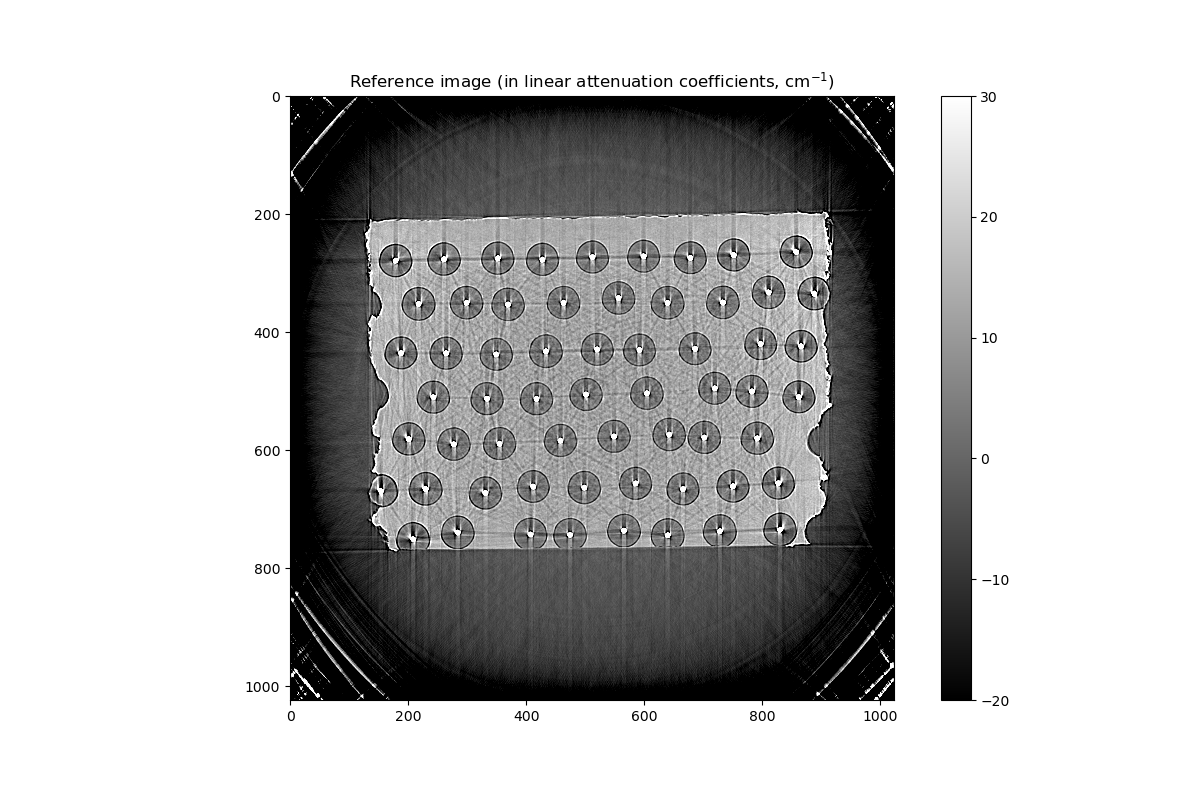
\includegraphics{plots/reference_image_in_mu.png}
\caption{Reference image (in linear attenuation coefficients}
\end{figure}

\hypertarget{normalise-the-image-data}{%
\section{Normalise the image data}\label{normalise-the-image-data}}

Zero-mean, unit-variance normalisation is applied to use the reference
images in objective functions and perform the registration. Note that it
is called standardisation (or Z-score Normalisation) in machine
learning. It is computed as follows:

\[\mathbf{m}_o=\frac{\mathbf{m}-\bar{m}}{\sigma_m}\]

where \(\mathbf{m}_o\) is the image after normalisation of Image
\(\mathbf{m}\), \(\bar{m}\) is the average pixel value of Image
\(\mathbf{m}\), and \(\sigma_m\) its standard deviation. After
normalisation, the average pixel value is null and the standard
deviation of pixel values is equal to one.

We define a function to apply this:

    \begin{tcolorbox}[breakable, size=fbox, boxrule=1pt, pad at break*=1mm,colback=cellbackground, colframe=cellborder]
\prompt{In}{incolor}{15}{\boxspacing}
\begin{Verbatim}[commandchars=\\\{\}]
\PY{k}{def} \PY{n+nf}{standardisation}\PY{p}{(}\PY{n}{I}\PY{p}{)}\PY{p}{:}
    \PY{n}{image} \PY{o}{=} \PY{n}{copy}\PY{o}{.}\PY{n}{deepcopy}\PY{p}{(}\PY{n}{I}\PY{p}{)}\PY{p}{;}

    \PY{c+c1}{\PYZsh{} Sometimes the CT reconstruction algorithm create NaN on}
    \PY{c+c1}{\PYZsh{} the top and right borders, we filter them out using}
    \PY{c+c1}{\PYZsh{} a median filter ignoring NaN}
    \PY{n}{nan\PYZus{}index} \PY{o}{=} \PY{n}{np}\PY{o}{.}\PY{n}{argwhere}\PY{p}{(}\PY{n}{np}\PY{o}{.}\PY{n}{isnan}\PY{p}{(}\PY{n}{image}\PY{p}{)}\PY{p}{)}\PY{p}{;}
    \PY{k}{if} \PY{n}{nan\PYZus{}index}\PY{o}{.}\PY{n}{shape}\PY{p}{[}\PY{l+m+mi}{0}\PY{p}{]}\PY{p}{:}
        \PY{n}{temp} \PY{o}{=} \PY{n}{np}\PY{o}{.}\PY{n}{pad}\PY{p}{(}\PY{n}{image}\PY{p}{,} \PY{l+m+mi}{1}\PY{p}{,} \PY{l+s+s2}{\PYZdq{}}\PY{l+s+s2}{edge}\PY{l+s+s2}{\PYZdq{}}\PY{p}{)}\PY{p}{;}

        \PY{k}{for} \PY{n}{index} \PY{o+ow}{in} \PY{n}{nan\PYZus{}index}\PY{p}{:}
            \PY{n}{roi} \PY{o}{=} \PY{n}{temp}\PY{p}{[}\PY{n}{index}\PY{p}{[}\PY{l+m+mi}{0}\PY{p}{]}\PY{o}{\PYZhy{}}\PY{l+m+mi}{1}\PY{o}{+}\PY{l+m+mi}{1}\PY{p}{:}\PY{n}{index}\PY{p}{[}\PY{l+m+mi}{0}\PY{p}{]}\PY{o}{+}\PY{l+m+mi}{1}\PY{o}{+}\PY{l+m+mi}{2}\PY{p}{,} \PY{n}{index}\PY{p}{[}\PY{l+m+mi}{1}\PY{p}{]}\PY{o}{\PYZhy{}}\PY{l+m+mi}{1}\PY{o}{+}\PY{l+m+mi}{1}\PY{p}{:}\PY{n}{index}\PY{p}{[}\PY{l+m+mi}{1}\PY{p}{]}\PY{o}{+}\PY{l+m+mi}{1}\PY{o}{+}\PY{l+m+mi}{2}\PY{p}{]}\PY{p}{;}
            \PY{n}{image}\PY{p}{[}\PY{n}{index}\PY{p}{[}\PY{l+m+mi}{0}\PY{p}{]}\PY{p}{,} \PY{n}{index}\PY{p}{[}\PY{l+m+mi}{1}\PY{p}{]}\PY{p}{]} \PY{o}{=} \PY{n}{np}\PY{o}{.}\PY{n}{nanmedian}\PY{p}{(}\PY{n}{roi}\PY{p}{)}\PY{p}{;}

    \PY{k}{return} \PY{p}{(}\PY{n}{image} \PY{o}{\PYZhy{}} \PY{n}{image}\PY{o}{.}\PY{n}{mean}\PY{p}{(}\PY{p}{)}\PY{p}{)} \PY{o}{/} \PY{n}{image}\PY{o}{.}\PY{n}{std}\PY{p}{(}\PY{p}{)}\PY{p}{;}
\end{Verbatim}
\end{tcolorbox}

    Normalise the reference sinogram and CT slice

    \begin{tcolorbox}[breakable, size=fbox, boxrule=1pt, pad at break*=1mm,colback=cellbackground, colframe=cellborder]
\prompt{In}{incolor}{16}{\boxspacing}
\begin{Verbatim}[commandchars=\\\{\}]
\PY{n}{normalised\PYZus{}reference\PYZus{}sinogram} \PY{o}{=} \PY{n}{standardisation}\PY{p}{(}\PY{n}{reference\PYZus{}sinogram}\PY{p}{)}\PY{p}{;}
\PY{n}{normalised\PYZus{}reference\PYZus{}CT}       \PY{o}{=} \PY{n}{standardisation}\PY{p}{(}\PY{n}{reference\PYZus{}CT}\PY{p}{)}\PY{p}{;}
\end{Verbatim}
\end{tcolorbox}

    \hypertarget{set-the-x-ray-simulation-environment}{%
\section{Set the X-ray simulation
environment}\label{set-the-x-ray-simulation-environment}}

    First we create an OpenGL context, here using EGL, i.e.~no window.

    \begin{tcolorbox}[breakable, size=fbox, boxrule=1pt, pad at break*=1mm,colback=cellbackground, colframe=cellborder]
\prompt{In}{incolor}{17}{\boxspacing}
\begin{Verbatim}[commandchars=\\\{\}]
\PY{n}{gvxr}\PY{o}{.}\PY{n}{createWindow}\PY{p}{(}\PY{l+m+mi}{0}\PY{p}{,} \PY{l+m+mi}{1}\PY{p}{,} \PY{l+s+s2}{\PYZdq{}}\PY{l+s+s2}{EGL}\PY{l+s+s2}{\PYZdq{}}\PY{p}{)}\PY{p}{;}
\PY{n}{gvxr}\PY{o}{.}\PY{n}{setWindowSize}\PY{p}{(}\PY{l+m+mi}{512}\PY{p}{,} \PY{l+m+mi}{512}\PY{p}{)}\PY{p}{;}
\end{Verbatim}
\end{tcolorbox}

    We set the parameters of the X-ray detector (flat pannel), e.g.~number
of pixels, pixel, spacing, position and orientation:

\begin{figure}
\centering
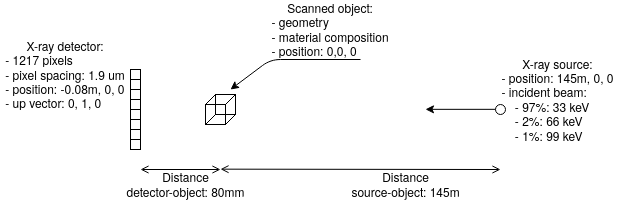
\includegraphics{./3d_scene.png}
\caption{3D scene to be simulated using gVirtualXray}
\end{figure}

    \begin{tcolorbox}[breakable, size=fbox, boxrule=1pt, pad at break*=1mm,colback=cellbackground, colframe=cellborder]
\prompt{In}{incolor}{18}{\boxspacing}
\begin{Verbatim}[commandchars=\\\{\}]
\PY{n}{detector\PYZus{}width\PYZus{}in\PYZus{}pixels} \PY{o}{=} \PY{n}{reference\PYZus{}sinogram}\PY{o}{.}\PY{n}{shape}\PY{p}{[}\PY{l+m+mi}{2}\PY{p}{]}\PY{p}{;}
\PY{n}{detector\PYZus{}height\PYZus{}in\PYZus{}pixels} \PY{o}{=} \PY{l+m+mi}{1}\PY{p}{;}
\PY{n}{distance\PYZus{}object\PYZus{}detector\PYZus{}in\PYZus{}m} \PY{o}{=}    \PY{l+m+mf}{0.08}\PY{p}{;} \PY{c+c1}{\PYZsh{} = 80 mm}

\PY{n}{gvxr}\PY{o}{.}\PY{n}{setDetectorPosition}\PY{p}{(}\PY{o}{\PYZhy{}}\PY{n}{distance\PYZus{}object\PYZus{}detector\PYZus{}in\PYZus{}m}\PY{p}{,} \PY{l+m+mf}{0.0}\PY{p}{,} \PY{l+m+mf}{0.0}\PY{p}{,} \PY{l+s+s2}{\PYZdq{}}\PY{l+s+s2}{m}\PY{l+s+s2}{\PYZdq{}}\PY{p}{)}\PY{p}{;}
\PY{n}{gvxr}\PY{o}{.}\PY{n}{setDetectorUpVector}\PY{p}{(}\PY{l+m+mi}{0}\PY{p}{,} \PY{l+m+mi}{1}\PY{p}{,} \PY{l+m+mi}{0}\PY{p}{)}\PY{p}{;}
\PY{n}{gvxr}\PY{o}{.}\PY{n}{setDetectorNumberOfPixels}\PY{p}{(}\PY{n}{detector\PYZus{}width\PYZus{}in\PYZus{}pixels}\PY{p}{,} \PY{n}{detector\PYZus{}height\PYZus{}in\PYZus{}pixels}\PY{p}{)}\PY{p}{;}
\PY{n}{gvxr}\PY{o}{.}\PY{n}{setDetectorPixelSize}\PY{p}{(}\PY{n}{pixel\PYZus{}spacing\PYZus{}in\PYZus{}micrometre}\PY{p}{,} \PY{n}{pixel\PYZus{}spacing\PYZus{}in\PYZus{}micrometre}\PY{p}{,} \PY{l+s+s2}{\PYZdq{}}\PY{l+s+s2}{micrometer}\PY{l+s+s2}{\PYZdq{}}\PY{p}{)}\PY{p}{;}
\end{Verbatim}
\end{tcolorbox}

    And the source parameters (beam shape, source position)

    \begin{tcolorbox}[breakable, size=fbox, boxrule=1pt, pad at break*=1mm,colback=cellbackground, colframe=cellborder]
\prompt{In}{incolor}{19}{\boxspacing}
\begin{Verbatim}[commandchars=\\\{\}]
\PY{c+c1}{\PYZsh{} Set up the beam}
\PY{n}{distance\PYZus{}source\PYZus{}detector\PYZus{}in\PYZus{}m}  \PY{o}{=} \PY{l+m+mf}{145.0}\PY{p}{;}

\PY{n}{gvxr}\PY{o}{.}\PY{n}{setSourcePosition}\PY{p}{(}\PY{n}{distance\PYZus{}source\PYZus{}detector\PYZus{}in\PYZus{}m} \PY{o}{\PYZhy{}} \PY{n}{distance\PYZus{}object\PYZus{}detector\PYZus{}in\PYZus{}m}\PY{p}{,}  \PY{l+m+mf}{0.0}\PY{p}{,} \PY{l+m+mf}{0.0}\PY{p}{,} \PY{l+s+s2}{\PYZdq{}}\PY{l+s+s2}{m}\PY{l+s+s2}{\PYZdq{}}\PY{p}{)}\PY{p}{;}
\PY{n}{gvxr}\PY{o}{.}\PY{n}{usePointSource}\PY{p}{(}\PY{p}{)}\PY{p}{;}
\PY{c+c1}{\PYZsh{} gvxr.useParallelBeam();}
\end{Verbatim}
\end{tcolorbox}

    The beam spectrum. Here we have a polychromatic beam, with 97\% of the
photons at 33 keV, 2\% at 66 keV and 1\% at 99 keV.

    \begin{tcolorbox}[breakable, size=fbox, boxrule=1pt, pad at break*=1mm,colback=cellbackground, colframe=cellborder]
\prompt{In}{incolor}{20}{\boxspacing}
\begin{Verbatim}[commandchars=\\\{\}]
\PY{n}{energy\PYZus{}spectrum} \PY{o}{=} \PY{p}{[}\PY{p}{(}\PY{l+m+mi}{33}\PY{p}{,} \PY{l+m+mf}{0.97}\PY{p}{,} \PY{l+s+s2}{\PYZdq{}}\PY{l+s+s2}{keV}\PY{l+s+s2}{\PYZdq{}}\PY{p}{)}\PY{p}{,} \PY{p}{(}\PY{l+m+mi}{66}\PY{p}{,} \PY{l+m+mf}{0.02}\PY{p}{,} \PY{l+s+s2}{\PYZdq{}}\PY{l+s+s2}{keV}\PY{l+s+s2}{\PYZdq{}}\PY{p}{)}\PY{p}{,} \PY{p}{(}\PY{l+m+mi}{99}\PY{p}{,} \PY{l+m+mf}{0.01}\PY{p}{,} \PY{l+s+s2}{\PYZdq{}}\PY{l+s+s2}{keV}\PY{l+s+s2}{\PYZdq{}}\PY{p}{)}\PY{p}{]}\PY{p}{;}

\PY{k}{for} \PY{n}{energy}\PY{p}{,} \PY{n}{percentage}\PY{p}{,} \PY{n}{unit} \PY{o+ow}{in} \PY{n}{energy\PYZus{}spectrum}\PY{p}{:}
    \PY{n}{gvxr}\PY{o}{.}\PY{n}{addEnergyBinToSpectrum}\PY{p}{(}\PY{n}{energy}\PY{p}{,} \PY{n}{unit}\PY{p}{,} \PY{n}{percentage}\PY{p}{)}\PY{p}{;}
\end{Verbatim}
\end{tcolorbox}

    Plot the beam spectrum using Matplotlib

    \begin{tcolorbox}[breakable, size=fbox, boxrule=1pt, pad at break*=1mm,colback=cellbackground, colframe=cellborder]
\prompt{In}{incolor}{21}{\boxspacing}
\begin{Verbatim}[commandchars=\\\{\}]
\PY{n}{energies\PYZus{}in\PYZus{}keV} \PY{o}{=} \PY{p}{[}\PY{p}{]}\PY{p}{;}
\PY{n}{weights} \PY{o}{=} \PY{p}{[}\PY{p}{]}\PY{p}{;}

\PY{k}{for} \PY{n}{energy}\PY{p}{,} \PY{n}{percentage}\PY{p}{,} \PY{n}{unit} \PY{o+ow}{in} \PY{n}{energy\PYZus{}spectrum}\PY{p}{:}
    \PY{n}{weights}\PY{o}{.}\PY{n}{append}\PY{p}{(}\PY{n}{percentage}\PY{p}{)}\PY{p}{;}
    \PY{n}{energies\PYZus{}in\PYZus{}keV}\PY{o}{.}\PY{n}{append}\PY{p}{(}\PY{n}{energy} \PY{o}{*} \PY{n}{gvxr}\PY{o}{.}\PY{n}{getUnitOfEnergy}\PY{p}{(}\PY{n}{unit}\PY{p}{)} \PY{o}{/} \PY{n}{gvxr}\PY{o}{.}\PY{n}{getUnitOfEnergy}\PY{p}{(}\PY{l+s+s2}{\PYZdq{}}\PY{l+s+s2}{keV}\PY{l+s+s2}{\PYZdq{}}\PY{p}{)}\PY{p}{)}\PY{p}{;}

\PY{n}{fig}\PY{o}{=}\PY{n}{plt}\PY{o}{.}\PY{n}{figure}\PY{p}{(}\PY{p}{)}\PY{p}{;}
\PY{n}{plt}\PY{o}{.}\PY{n}{xlabel}\PY{p}{(}\PY{l+s+s2}{\PYZdq{}}\PY{l+s+s2}{Energy bin (in keV)}\PY{l+s+s2}{\PYZdq{}}\PY{p}{)}\PY{p}{;}
\PY{n}{plt}\PY{o}{.}\PY{n}{ylabel}\PY{p}{(}\PY{l+s+s2}{\PYZdq{}}\PY{l+s+s2}{Relative weight}\PY{l+s+s2}{\PYZdq{}}\PY{p}{)}\PY{p}{;}
\PY{n}{plt}\PY{o}{.}\PY{n}{xticks}\PY{p}{(}\PY{n}{energies\PYZus{}in\PYZus{}keV}\PY{p}{)}\PY{p}{;}
\PY{n}{plt}\PY{o}{.}\PY{n}{yticks}\PY{p}{(}\PY{n}{weights}\PY{p}{)}\PY{p}{;}
\PY{n}{plt}\PY{o}{.}\PY{n}{title}\PY{p}{(}\PY{l+s+s2}{\PYZdq{}}\PY{l+s+s2}{Incident beam spectrum}\PY{l+s+s2}{\PYZdq{}}\PY{p}{)}\PY{p}{;}
\PY{n}{plt}\PY{o}{.}\PY{n}{bar}\PY{p}{(}\PY{n}{energies\PYZus{}in\PYZus{}keV}\PY{p}{,} \PY{n}{weights}\PY{p}{)}\PY{p}{;}
\PY{n}{plt}\PY{o}{.}\PY{n}{savefig}\PY{p}{(}\PY{l+s+s1}{\PYZsq{}}\PY{l+s+s1}{plots/beam\PYZus{}spectrum.pdf}\PY{l+s+s1}{\PYZsq{}}\PY{p}{)}\PY{p}{;}
\PY{n}{plt}\PY{o}{.}\PY{n}{savefig}\PY{p}{(}\PY{l+s+s1}{\PYZsq{}}\PY{l+s+s1}{plots/beam\PYZus{}spectrum.png}\PY{l+s+s1}{\PYZsq{}}\PY{p}{)}\PY{p}{;}
\end{Verbatim}
\end{tcolorbox}

    \begin{figure}
\centering
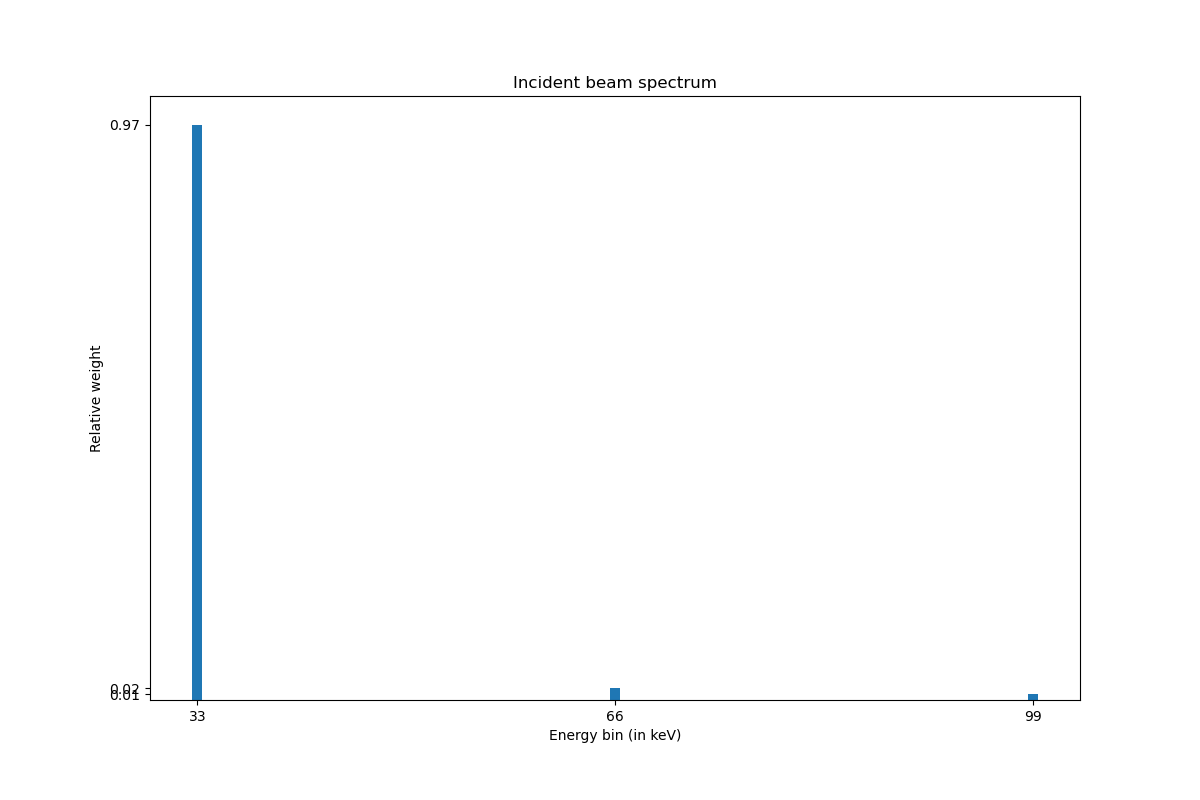
\includegraphics{plots/beam_spectrum.png}
\caption{Incident beam spectrum}
\end{figure}

The material properties (chemical composition and density)

    \begin{tcolorbox}[breakable, size=fbox, boxrule=1pt, pad at break*=1mm,colback=cellbackground, colframe=cellborder]
\prompt{In}{incolor}{22}{\boxspacing}
\begin{Verbatim}[commandchars=\\\{\}]
\PY{n}{fibre\PYZus{}material} \PY{o}{=} \PY{p}{[}\PY{p}{(}\PY{l+s+s2}{\PYZdq{}}\PY{l+s+s2}{Si}\PY{l+s+s2}{\PYZdq{}}\PY{p}{,} \PY{l+m+mf}{0.5}\PY{p}{)}\PY{p}{,} \PY{p}{(}\PY{l+s+s2}{\PYZdq{}}\PY{l+s+s2}{C}\PY{l+s+s2}{\PYZdq{}}\PY{p}{,} \PY{l+m+mf}{0.5}\PY{p}{)}\PY{p}{]}\PY{p}{;}
\PY{n}{fibre\PYZus{}density} \PY{o}{=} \PY{l+m+mf}{3.2}\PY{p}{;} \PY{c+c1}{\PYZsh{} g/cm3}

\PY{n}{core\PYZus{}radius} \PY{o}{=} \PY{l+m+mi}{30} \PY{o}{/} \PY{l+m+mi}{2}\PY{p}{;} \PY{c+c1}{\PYZsh{} um}
\PY{n}{core\PYZus{}material} \PY{o}{=} \PY{p}{[}\PY{p}{(}\PY{l+s+s2}{\PYZdq{}}\PY{l+s+s2}{W}\PY{l+s+s2}{\PYZdq{}}\PY{p}{,} \PY{l+m+mi}{1}\PY{p}{)}\PY{p}{]}\PY{p}{;}

\PY{n}{g\PYZus{}matrix\PYZus{}width} \PY{o}{=} \PY{l+m+mi}{0}\PY{p}{;}
\PY{n}{g\PYZus{}matrix\PYZus{}height} \PY{o}{=} \PY{l+m+mi}{0}\PY{p}{;}
\PY{n}{g\PYZus{}matrix\PYZus{}x} \PY{o}{=} \PY{l+m+mi}{0}\PY{p}{;}
\PY{n}{g\PYZus{}matrix\PYZus{}y} \PY{o}{=} \PY{l+m+mi}{0}\PY{p}{;}
\PY{n}{matrix\PYZus{}material} \PY{o}{=} \PY{p}{[}\PY{p}{(}\PY{l+s+s2}{\PYZdq{}}\PY{l+s+s2}{Ti}\PY{l+s+s2}{\PYZdq{}}\PY{p}{,} \PY{l+m+mf}{0.9}\PY{p}{)}\PY{p}{,} \PY{p}{(}\PY{l+s+s2}{\PYZdq{}}\PY{l+s+s2}{Al}\PY{l+s+s2}{\PYZdq{}}\PY{p}{,} \PY{l+m+mf}{0.06}\PY{p}{)}\PY{p}{,} \PY{p}{(}\PY{l+s+s2}{\PYZdq{}}\PY{l+s+s2}{V}\PY{l+s+s2}{\PYZdq{}}\PY{p}{,} \PY{l+m+mf}{0.04}\PY{p}{)}\PY{p}{]}\PY{p}{;}
\PY{n}{matrix\PYZus{}density} \PY{o}{=} \PY{l+m+mf}{4.42} \PY{c+c1}{\PYZsh{} g/cm3}
\end{Verbatim}
\end{tcolorbox}

    \hypertarget{the-lsf}{%
\subsection{The LSF}\label{the-lsf}}

In a previous study, we experimentally measured the impulse response of
the detector as the line spread function (LSF):

F.P. Vidal, J.M. Létang, G. Peix, P. Cloetens, Investigation of artefact
sources in synchrotron microtomography via virtual X-ray imaging,
\emph{Nuclear Instruments and Methods in Physics Research Section B:
Beam Interactions with Materials and Atoms}, Volume 234, Issue 3, 2005,
Pages 333-348, ISSN 0168-583X, DOI \url{10.1016/j.nimb.2005.02.003}.

We use this model during the initial steps of the registration. The LSF
model will be tuned in one of the final steps of the registration.

    \begin{tcolorbox}[breakable, size=fbox, boxrule=1pt, pad at break*=1mm,colback=cellbackground, colframe=cellborder]
\prompt{In}{incolor}{23}{\boxspacing}
\begin{Verbatim}[commandchars=\\\{\}]
\PY{n}{t} \PY{o}{=} \PY{n}{np}\PY{o}{.}\PY{n}{arange}\PY{p}{(}\PY{o}{\PYZhy{}}\PY{l+m+mf}{20.}\PY{p}{,} \PY{l+m+mf}{21.}\PY{p}{,} \PY{l+m+mf}{1.}\PY{p}{)}\PY{p}{;}
\PY{n}{lsf\PYZus{}kernel}\PY{o}{=}\PY{n}{lsf}\PY{p}{(}\PY{n}{t}\PY{o}{*}\PY{l+m+mi}{41}\PY{p}{)}\PY{o}{/}\PY{n}{lsf}\PY{p}{(}\PY{l+m+mi}{0}\PY{p}{)}\PY{p}{;}
\PY{n}{lsf\PYZus{}kernel}\PY{o}{/}\PY{o}{=}\PY{n}{lsf\PYZus{}kernel}\PY{o}{.}\PY{n}{sum}\PY{p}{(}\PY{p}{)}\PY{p}{;}
\end{Verbatim}
\end{tcolorbox}

    Plot the LSF using Matplotlib

    \begin{tcolorbox}[breakable, size=fbox, boxrule=1pt, pad at break*=1mm,colback=cellbackground, colframe=cellborder]
\prompt{In}{incolor}{24}{\boxspacing}
\begin{Verbatim}[commandchars=\\\{\}]
\PY{n}{fig}\PY{o}{=}\PY{n}{plt}\PY{o}{.}\PY{n}{figure}\PY{p}{(}\PY{p}{)}\PY{p}{;}
\PY{n}{plt}\PY{o}{.}\PY{n}{title}\PY{p}{(}\PY{l+s+s2}{\PYZdq{}}\PY{l+s+s2}{Response of the detector (LSF)}\PY{l+s+s2}{\PYZdq{}}\PY{p}{)}\PY{p}{;}
\PY{n}{plt}\PY{o}{.}\PY{n}{plot}\PY{p}{(}\PY{n}{t}\PY{p}{,} \PY{n}{lsf\PYZus{}kernel}\PY{p}{)}\PY{p}{;}
\PY{n}{plt}\PY{o}{.}\PY{n}{savefig}\PY{p}{(}\PY{l+s+s1}{\PYZsq{}}\PY{l+s+s1}{plots/LSF.pdf}\PY{l+s+s1}{\PYZsq{}}\PY{p}{)}\PY{p}{;}
\PY{n}{plt}\PY{o}{.}\PY{n}{savefig}\PY{p}{(}\PY{l+s+s1}{\PYZsq{}}\PY{l+s+s1}{plots/LSF.png}\PY{l+s+s1}{\PYZsq{}}\PY{p}{)}\PY{p}{;}
\end{Verbatim}
\end{tcolorbox}

    \begin{figure}
\centering
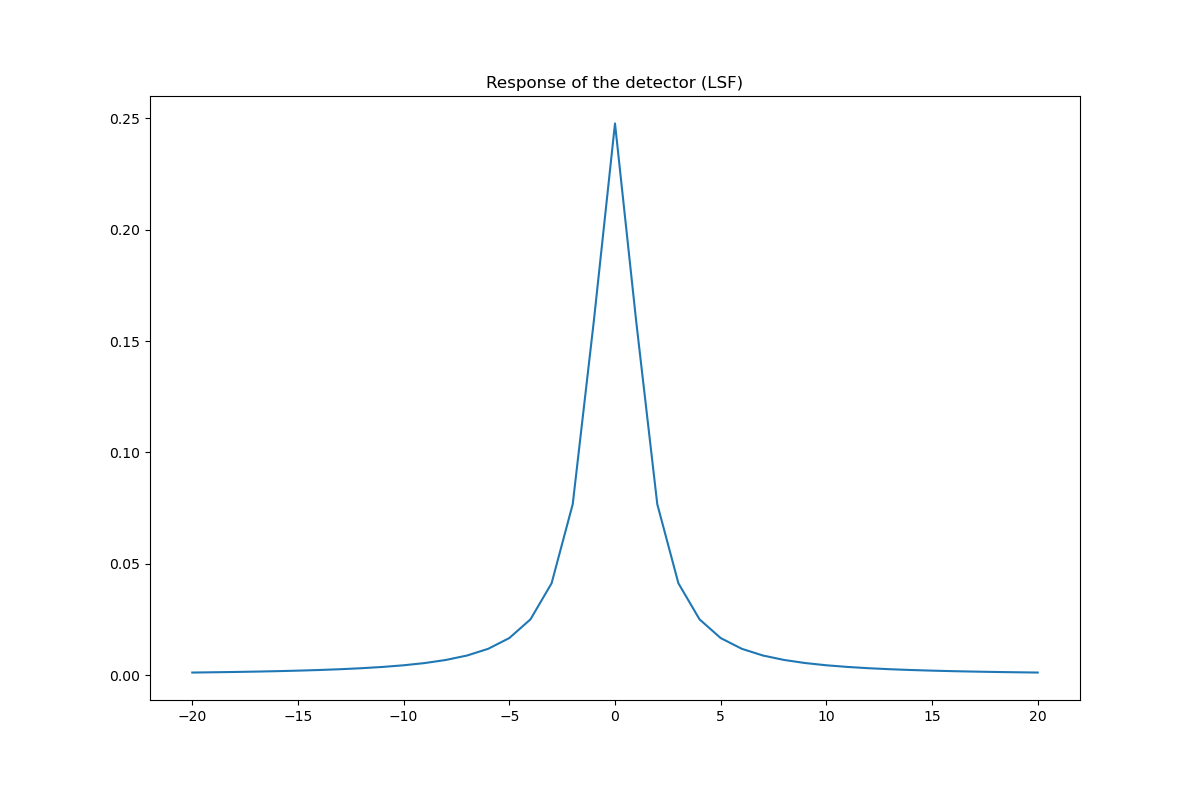
\includegraphics{plots/LSF.png}
\caption{Response of the detector (LSF)}
\end{figure}

\hypertarget{find-circles-to-identify-the-centre-of-fibres}{%
\section{Find circles to identify the centre of
fibres}\label{find-circles-to-identify-the-centre-of-fibres}}

We can use the Hoguh transform to detect where circles are in the image.
However, the input image in OpenCV's function must be in UINT. We blur
it using a bilateral filter (an edge-preserving smoothing filter).

    \hypertarget{convert-the-image-to-uint}{%
\subsection{Convert the image to
UINT}\label{convert-the-image-to-uint}}

    We first create a function to convert images in floating point numbers
into UINT.

    \begin{tcolorbox}[breakable, size=fbox, boxrule=1pt, pad at break*=1mm,colback=cellbackground, colframe=cellborder]
\prompt{In}{incolor}{25}{\boxspacing}
\begin{Verbatim}[commandchars=\\\{\}]
\PY{k}{def} \PY{n+nf}{float2uint8}\PY{p}{(}\PY{n}{anImage}\PY{p}{,} \PY{n}{min\PYZus{}threshold} \PY{o}{=} \PY{k+kc}{None}\PY{p}{,} \PY{n}{max\PYZus{}threshold} \PY{o}{=} \PY{k+kc}{None}\PY{p}{)}\PY{p}{:}
    
    \PY{n}{uchar\PYZus{}image} \PY{o}{=} \PY{n}{copy}\PY{o}{.}\PY{n}{deepcopy}\PY{p}{(}\PY{n}{anImage}\PY{p}{)}\PY{p}{;}

    \PY{k}{if} \PY{n+nb}{isinstance}\PY{p}{(}\PY{n}{min\PYZus{}threshold}\PY{p}{,} \PY{n}{NoneType}\PY{p}{)}\PY{p}{:}
        \PY{n}{min\PYZus{}threshold} \PY{o}{=} \PY{n}{np}\PY{o}{.}\PY{n}{min}\PY{p}{(}\PY{n}{uchar\PYZus{}image}\PY{p}{)}\PY{p}{;}

    \PY{k}{if} \PY{n+nb}{isinstance}\PY{p}{(}\PY{n}{max\PYZus{}threshold}\PY{p}{,} \PY{n}{NoneType}\PY{p}{)}\PY{p}{:}
        \PY{n}{max\PYZus{}threshold} \PY{o}{=} \PY{n}{np}\PY{o}{.}\PY{n}{max}\PY{p}{(}\PY{n}{uchar\PYZus{}image}\PY{p}{)}\PY{p}{;}
        
    \PY{n}{uchar\PYZus{}image}\PY{p}{[}\PY{n}{uchar\PYZus{}image} \PY{o}{\PYZlt{}} \PY{n}{min\PYZus{}threshold}\PY{p}{]} \PY{o}{=} \PY{n}{min\PYZus{}threshold}\PY{p}{;}
    \PY{n}{uchar\PYZus{}image}\PY{p}{[}\PY{n}{uchar\PYZus{}image} \PY{o}{\PYZgt{}} \PY{n}{max\PYZus{}threshold}\PY{p}{]} \PY{o}{=} \PY{n}{max\PYZus{}threshold}\PY{p}{;}

    \PY{n}{uchar\PYZus{}image} \PY{o}{\PYZhy{}}\PY{o}{=} \PY{n}{min\PYZus{}threshold}\PY{p}{;}
    \PY{n}{uchar\PYZus{}image} \PY{o}{/}\PY{o}{=} \PY{n}{max\PYZus{}threshold} \PY{o}{\PYZhy{}} \PY{n}{min\PYZus{}threshold}\PY{p}{;}
    \PY{n}{uchar\PYZus{}image} \PY{o}{*}\PY{o}{=} \PY{l+m+mi}{255}\PY{p}{;}
    
    \PY{k}{return} \PY{n}{uchar\PYZus{}image}\PY{o}{.}\PY{n}{astype}\PY{p}{(}\PY{n}{np}\PY{o}{.}\PY{n}{uint8}\PY{p}{)}\PY{p}{;}
\end{Verbatim}
\end{tcolorbox}

    We blur the CT scan using a bilateral filter. It preserves edges.

    \begin{tcolorbox}[breakable, size=fbox, boxrule=1pt, pad at break*=1mm,colback=cellbackground, colframe=cellborder]
\prompt{In}{incolor}{26}{\boxspacing}
\begin{Verbatim}[commandchars=\\\{\}]
\PY{n}{uint8\PYZus{}reference\PYZus{}CT} \PY{o}{=} \PY{n}{float2uint8}\PY{p}{(}\PY{n}{reference\PYZus{}CT}\PY{p}{,} \PY{l+m+mi}{0}\PY{p}{,} \PY{l+m+mi}{300}\PY{p}{)}\PY{p}{;}
\PY{n}{blurred\PYZus{}reference\PYZus{}CT} \PY{o}{=} \PY{n}{cv2}\PY{o}{.}\PY{n}{bilateralFilter}\PY{p}{(}\PY{n}{uint8\PYZus{}reference\PYZus{}CT}\PY{p}{,} \PY{l+m+mi}{9}\PY{p}{,} \PY{l+m+mi}{75}\PY{p}{,} \PY{l+m+mi}{75}\PY{p}{)}\PY{p}{;}

\PY{n}{saveMHA}\PY{p}{(}\PY{l+s+s1}{\PYZsq{}}\PY{l+s+s1}{outputs/blurred\PYZus{}reference\PYZus{}CT.mha}\PY{l+s+s1}{\PYZsq{}}\PY{p}{,} \PY{n}{blurred\PYZus{}reference\PYZus{}CT}\PY{p}{,} \PY{p}{[}\PY{n}{pixel\PYZus{}spacing\PYZus{}in\PYZus{}mm}\PY{p}{,} \PY{n}{angular\PYZus{}step}\PY{p}{,} \PY{n}{pixel\PYZus{}spacing\PYZus{}in\PYZus{}mm}\PY{p}{]}\PY{p}{)}\PY{p}{;}
\end{Verbatim}
\end{tcolorbox}

    \hypertarget{apply-the-hough-transform}{%
\subsection{Apply the Hough
transform}\label{apply-the-hough-transform}}

As the fibres and the cores correspond to circles in the CT images, the
obvious technique to try is the Hough Circle Transform (HCT). It is a
feature extraction technique used in image analysis that can output a
list of circles (centres and radii).

    \begin{tcolorbox}[breakable, size=fbox, boxrule=1pt, pad at break*=1mm,colback=cellbackground, colframe=cellborder]
\prompt{In}{incolor}{27}{\boxspacing}
\begin{Verbatim}[commandchars=\\\{\}]
\PY{n}{circles} \PY{o}{=} \PY{n}{cv2}\PY{o}{.}\PY{n}{HoughCircles}\PY{p}{(}\PY{n}{blurred\PYZus{}reference\PYZus{}CT}\PY{p}{,} \PY{n}{cv2}\PY{o}{.}\PY{n}{HOUGH\PYZus{}GRADIENT}\PY{p}{,} \PY{l+m+mi}{2}\PY{p}{,} \PY{l+m+mi}{80}\PY{p}{,}
                            \PY{n}{param1}\PY{o}{=}\PY{l+m+mi}{150}\PY{p}{,} \PY{n}{param2}\PY{o}{=}\PY{l+m+mi}{5}\PY{p}{,} \PY{n}{minRadius}\PY{o}{=}\PY{l+m+mi}{5}\PY{p}{,} \PY{n}{maxRadius}\PY{o}{=}\PY{l+m+mi}{15}\PY{p}{)}\PY{p}{;}
\end{Verbatim}
\end{tcolorbox}

    \hypertarget{overlay-the-detected-circles-on-the-top-of-the-image}{%
\subsection{Overlay the detected circles on the top of the
image}\label{overlay-the-detected-circles-on-the-top-of-the-image}}

    \begin{tcolorbox}[breakable, size=fbox, boxrule=1pt, pad at break*=1mm,colback=cellbackground, colframe=cellborder]
\prompt{In}{incolor}{28}{\boxspacing}
\begin{Verbatim}[commandchars=\\\{\}]
\PY{n}{cimg} \PY{o}{=} \PY{n}{cv2}\PY{o}{.}\PY{n}{cvtColor}\PY{p}{(}\PY{n}{blurred\PYZus{}reference\PYZus{}CT}\PY{p}{,} \PY{n}{cv2}\PY{o}{.}\PY{n}{COLOR\PYZus{}GRAY2BGR}\PY{p}{)}\PY{p}{;}
\PY{n}{circles} \PY{o}{=} \PY{n}{np}\PY{o}{.}\PY{n}{uint16}\PY{p}{(}\PY{n}{np}\PY{o}{.}\PY{n}{around}\PY{p}{(}\PY{n}{circles}\PY{p}{)}\PY{p}{)}\PY{p}{;}

\PY{k}{for} \PY{n}{i} \PY{o+ow}{in} \PY{n}{circles}\PY{p}{[}\PY{l+m+mi}{0}\PY{p}{,}\PY{p}{:}\PY{p}{]}\PY{p}{:}
    
    \PY{c+c1}{\PYZsh{} draw the outer circle}
    \PY{n}{cv2}\PY{o}{.}\PY{n}{circle}\PY{p}{(}\PY{n}{cimg}\PY{p}{,} \PY{p}{(}\PY{n}{i}\PY{p}{[}\PY{l+m+mi}{0}\PY{p}{]}\PY{p}{,} \PY{n}{i}\PY{p}{[}\PY{l+m+mi}{1}\PY{p}{]}\PY{p}{)}\PY{p}{,} \PY{n}{i}\PY{p}{[}\PY{l+m+mi}{2}\PY{p}{]}\PY{p}{,} \PY{p}{(}\PY{l+m+mi}{0}\PY{p}{,} \PY{l+m+mi}{255}\PY{p}{,} \PY{l+m+mi}{0}\PY{p}{)}\PY{p}{,} \PY{l+m+mi}{2}\PY{p}{)}\PY{p}{;}
    
    \PY{c+c1}{\PYZsh{} draw the center of the circle}
    \PY{n}{cv2}\PY{o}{.}\PY{n}{circle}\PY{p}{(}\PY{n}{cimg}\PY{p}{,} \PY{p}{(}\PY{n}{i}\PY{p}{[}\PY{l+m+mi}{0}\PY{p}{]}\PY{p}{,} \PY{n}{i}\PY{p}{[}\PY{l+m+mi}{1}\PY{p}{]}\PY{p}{)}\PY{p}{,} \PY{l+m+mi}{2}\PY{p}{,} \PY{p}{(}\PY{l+m+mi}{0}\PY{p}{,} \PY{l+m+mi}{0}\PY{p}{,} \PY{l+m+mi}{255}\PY{p}{)}\PY{p}{,} \PY{l+m+mi}{3}\PY{p}{)}\PY{p}{;}
\end{Verbatim}
\end{tcolorbox}

    \begin{tcolorbox}[breakable, size=fbox, boxrule=1pt, pad at break*=1mm,colback=cellbackground, colframe=cellborder]
\prompt{In}{incolor}{29}{\boxspacing}
\begin{Verbatim}[commandchars=\\\{\}]
\PY{n}{fig}\PY{o}{=}\PY{n}{plt}\PY{o}{.}\PY{n}{figure}\PY{p}{(}\PY{p}{)}\PY{p}{;}
\PY{n}{imgplot} \PY{o}{=} \PY{n}{plt}\PY{o}{.}\PY{n}{imshow}\PY{p}{(}\PY{n}{cimg}\PY{p}{)}\PY{p}{;}
\PY{n}{plt}\PY{o}{.}\PY{n}{title}\PY{p}{(}\PY{l+s+s2}{\PYZdq{}}\PY{l+s+s2}{Reference image and detected Tungsten cores}\PY{l+s+s2}{\PYZdq{}}\PY{p}{)}\PY{p}{;}
\PY{n}{plt}\PY{o}{.}\PY{n}{savefig}\PY{p}{(}\PY{l+s+s1}{\PYZsq{}}\PY{l+s+s1}{plots/fibre\PYZus{}detection\PYZus{}using\PYZus{}Hough\PYZus{}transform.pdf}\PY{l+s+s1}{\PYZsq{}}\PY{p}{)}\PY{p}{;}
\PY{n}{plt}\PY{o}{.}\PY{n}{savefig}\PY{p}{(}\PY{l+s+s1}{\PYZsq{}}\PY{l+s+s1}{plots/fibre\PYZus{}detection\PYZus{}using\PYZus{}Hough\PYZus{}transform.png}\PY{l+s+s1}{\PYZsq{}}\PY{p}{)}\PY{p}{;}
\end{Verbatim}
\end{tcolorbox}

    \begin{figure}
\centering
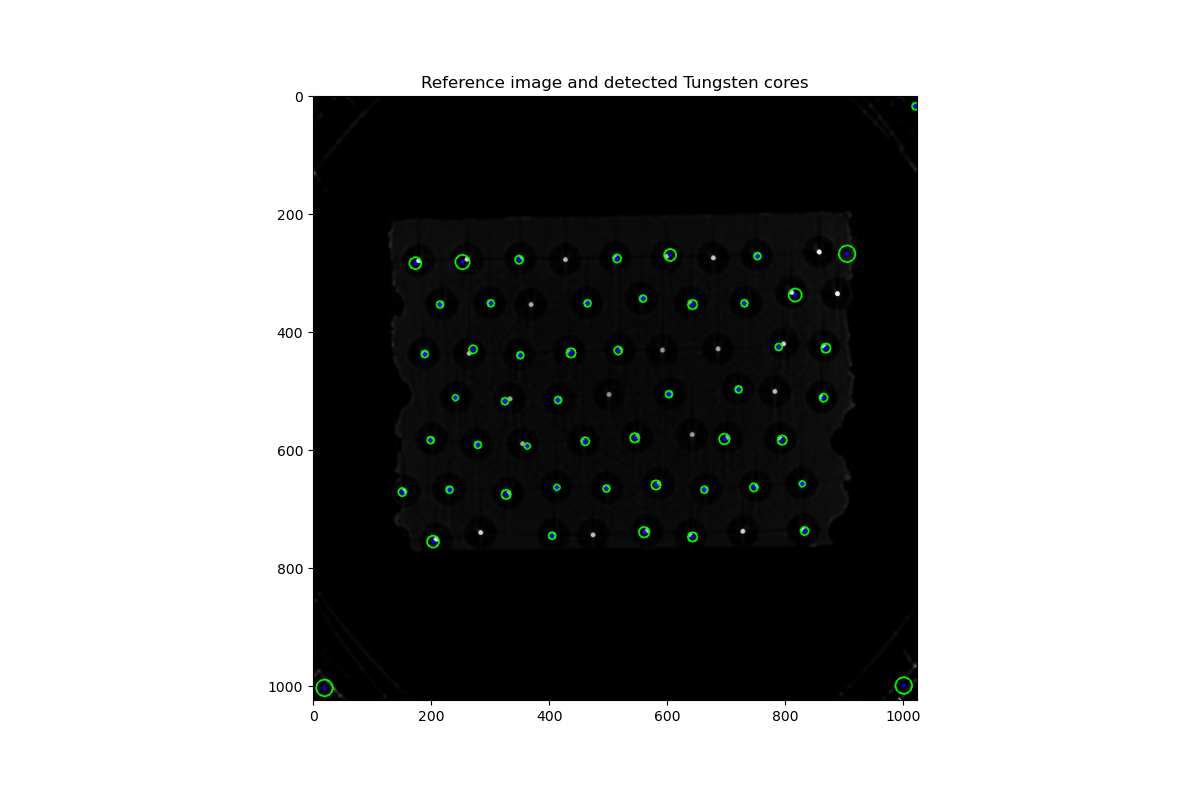
\includegraphics{plots/fibre_detection_using_Hough_transform.png}
\caption{Reference image and detected Tungsten cores using the Hough
Circle Transform}
\end{figure}

13 fibres were missed and many centres were misplaced. Controlling the
meta-parameters of the algorithm can be difficult to employ in a
fully-automatic registration framework. We will use another technique to
register the fibres, the popular Otsu's method. It creates a histogram
and uses a heuristic to determine a threshold value.

    \begin{tcolorbox}[breakable, size=fbox, boxrule=1pt, pad at break*=1mm,colback=cellbackground, colframe=cellborder]
\prompt{In}{incolor}{30}{\boxspacing}
\begin{Verbatim}[commandchars=\\\{\}]
\PY{c+c1}{\PYZsh{} Convert the numpy array in float32 into uint, then into a SITK image}
\PY{n}{volume} \PY{o}{=} \PY{n}{sitk}\PY{o}{.}\PY{n}{GetImageFromArray}\PY{p}{(}\PY{n}{blurred\PYZus{}reference\PYZus{}CT}\PY{p}{)}\PY{p}{;}
\PY{n}{volume}\PY{o}{.}\PY{n}{SetSpacing}\PY{p}{(}\PY{p}{[}\PY{n}{pixel\PYZus{}spacing\PYZus{}in\PYZus{}mm}\PY{p}{,} \PY{n}{pixel\PYZus{}spacing\PYZus{}in\PYZus{}mm}\PY{p}{,} \PY{n}{pixel\PYZus{}spacing\PYZus{}in\PYZus{}mm}\PY{p}{]}\PY{p}{)}\PY{p}{;}

\PY{c+c1}{\PYZsh{} Apply the Otsu\PYZsq{}s method}
\PY{n}{otsu\PYZus{}filter} \PY{o}{=} \PY{n}{sitk}\PY{o}{.}\PY{n}{OtsuThresholdImageFilter}\PY{p}{(}\PY{p}{)}\PY{p}{;}
\PY{n}{otsu\PYZus{}filter}\PY{o}{.}\PY{n}{SetInsideValue}\PY{p}{(}\PY{l+m+mi}{0}\PY{p}{)}\PY{p}{;}
\PY{n}{otsu\PYZus{}filter}\PY{o}{.}\PY{n}{SetOutsideValue}\PY{p}{(}\PY{l+m+mi}{1}\PY{p}{)}\PY{p}{;}
\PY{n}{seg} \PY{o}{=} \PY{n}{otsu\PYZus{}filter}\PY{o}{.}\PY{n}{Execute}\PY{p}{(}\PY{n}{volume}\PY{p}{)}\PY{p}{;}

\PY{c+c1}{\PYZsh{} Print the corresponding threshold}
\PY{n+nb}{print}\PY{p}{(}\PY{l+s+s2}{\PYZdq{}}\PY{l+s+s2}{Threshold:}\PY{l+s+s2}{\PYZdq{}}\PY{p}{,} \PY{n}{otsu\PYZus{}filter}\PY{o}{.}\PY{n}{GetThreshold}\PY{p}{(}\PY{p}{)}\PY{p}{)}\PY{p}{;}
\end{Verbatim}
\end{tcolorbox}

    \begin{Verbatim}[commandchars=\\\{\}]
Threshold: 91.0
    \end{Verbatim}

    \begin{tcolorbox}[breakable, size=fbox, boxrule=1pt, pad at break*=1mm,colback=cellbackground, colframe=cellborder]
\prompt{In}{incolor}{31}{\boxspacing}
\begin{Verbatim}[commandchars=\\\{\}]
\PY{n}{sitk}\PY{o}{.}\PY{n}{WriteImage}\PY{p}{(}\PY{n}{seg}\PY{p}{,} \PY{l+s+s2}{\PYZdq{}}\PY{l+s+s2}{outputs/cores\PYZus{}segmentation.mha}\PY{l+s+s2}{\PYZdq{}}\PY{p}{,} \PY{n}{useCompression}\PY{o}{=}\PY{k+kc}{True}\PY{p}{)}\PY{p}{;}
\end{Verbatim}
\end{tcolorbox}

    \begin{tcolorbox}[breakable, size=fbox, boxrule=1pt, pad at break*=1mm,colback=cellbackground, colframe=cellborder]
\prompt{In}{incolor}{32}{\boxspacing}
\begin{Verbatim}[commandchars=\\\{\}]
\PY{n}{fig} \PY{o}{=} \PY{n}{plt}\PY{o}{.}\PY{n}{figure}\PY{p}{(}\PY{p}{)}\PY{p}{;}
\PY{n}{imgplot} \PY{o}{=} \PY{n}{plt}\PY{o}{.}\PY{n}{imshow}\PY{p}{(}\PY{n}{sitk}\PY{o}{.}\PY{n}{GetArrayViewFromImage}\PY{p}{(}\PY{n}{sitk}\PY{o}{.}\PY{n}{LabelOverlay}\PY{p}{(}\PY{n}{volume}\PY{p}{,} \PY{n}{seg}\PY{p}{)}\PY{p}{)}\PY{p}{)}\PY{p}{;}
\PY{n}{plt}\PY{o}{.}\PY{n}{title}\PY{p}{(}\PY{l+s+s2}{\PYZdq{}}\PY{l+s+s2}{Reference image and detected Tungsten cores}\PY{l+s+s2}{\PYZdq{}}\PY{p}{)}\PY{p}{;}
\PY{n}{plt}\PY{o}{.}\PY{n}{savefig}\PY{p}{(}\PY{l+s+s1}{\PYZsq{}}\PY{l+s+s1}{plots/fibre\PYZus{}detection\PYZus{}using\PYZus{}otsu\PYZus{}method.pdf}\PY{l+s+s1}{\PYZsq{}}\PY{p}{)}\PY{p}{;}
\PY{n}{plt}\PY{o}{.}\PY{n}{savefig}\PY{p}{(}\PY{l+s+s1}{\PYZsq{}}\PY{l+s+s1}{plots/fibre\PYZus{}detection\PYZus{}using\PYZus{}otsu\PYZus{}method.png}\PY{l+s+s1}{\PYZsq{}}\PY{p}{)}\PY{p}{;}
\end{Verbatim}
\end{tcolorbox}

    \begin{figure}
\centering
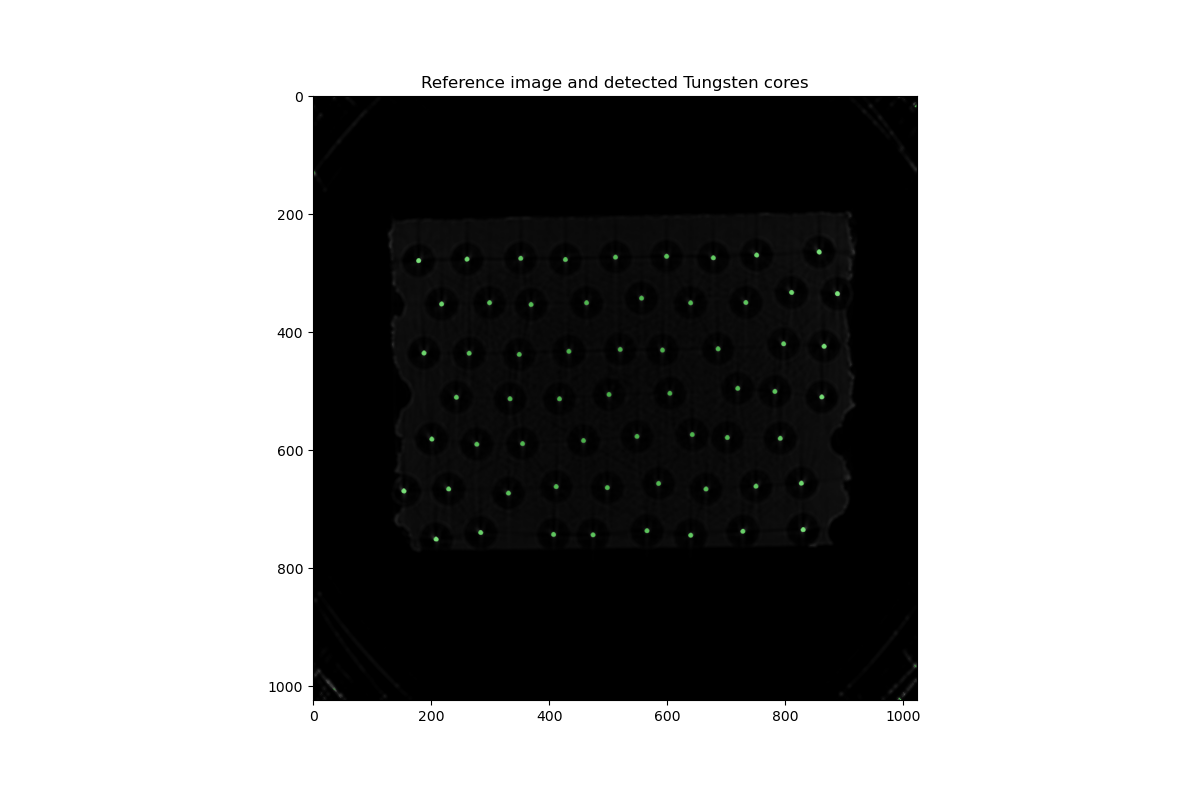
\includegraphics{plots/fibre_detection_using_otsu_method.png}
\caption{Reference image and detected Tungsten cores using the Otsu's
method}
\end{figure}

\hypertarget{clean-up}{%
\subsection{Clean up}\label{clean-up}}

    \begin{tcolorbox}[breakable, size=fbox, boxrule=1pt, pad at break*=1mm,colback=cellbackground, colframe=cellborder]
\prompt{In}{incolor}{33}{\boxspacing}
\begin{Verbatim}[commandchars=\\\{\}]
\PY{c+c1}{\PYZsh{} Clean\PYZhy{}up using mathematical morphology}
\PY{n}{cleaned\PYZus{}thresh\PYZus{}img} \PY{o}{=} \PY{n}{sitk}\PY{o}{.}\PY{n}{BinaryOpeningByReconstruction}\PY{p}{(}\PY{n}{seg}\PY{p}{,} \PY{p}{[}\PY{l+m+mi}{3}\PY{p}{,} \PY{l+m+mi}{3}\PY{p}{,} \PY{l+m+mi}{3}\PY{p}{]}\PY{p}{)}
\PY{n}{cleaned\PYZus{}thresh\PYZus{}img} \PY{o}{=} \PY{n}{sitk}\PY{o}{.}\PY{n}{BinaryClosingByReconstruction}\PY{p}{(}\PY{n}{cleaned\PYZus{}thresh\PYZus{}img}\PY{p}{,} \PY{p}{[}\PY{l+m+mi}{3}\PY{p}{,} \PY{l+m+mi}{3}\PY{p}{,} \PY{l+m+mi}{3}\PY{p}{]}\PY{p}{)}
\end{Verbatim}
\end{tcolorbox}

    \begin{tcolorbox}[breakable, size=fbox, boxrule=1pt, pad at break*=1mm,colback=cellbackground, colframe=cellborder]
\prompt{In}{incolor}{34}{\boxspacing}
\begin{Verbatim}[commandchars=\\\{\}]
\PY{n}{sitk}\PY{o}{.}\PY{n}{WriteImage}\PY{p}{(}\PY{n}{cleaned\PYZus{}thresh\PYZus{}img}\PY{p}{,} \PY{l+s+s2}{\PYZdq{}}\PY{l+s+s2}{outputs/cores\PYZus{}cleaned\PYZus{}segmentation.mha}\PY{l+s+s2}{\PYZdq{}}\PY{p}{,} \PY{n}{useCompression}\PY{o}{=}\PY{k+kc}{True}\PY{p}{)}\PY{p}{;}
\end{Verbatim}
\end{tcolorbox}

    \begin{tcolorbox}[breakable, size=fbox, boxrule=1pt, pad at break*=1mm,colback=cellbackground, colframe=cellborder]
\prompt{In}{incolor}{35}{\boxspacing}
\begin{Verbatim}[commandchars=\\\{\}]
\PY{n}{fig} \PY{o}{=} \PY{n}{plt}\PY{o}{.}\PY{n}{figure}\PY{p}{(}\PY{p}{)}\PY{p}{;}
\PY{n}{imgplot} \PY{o}{=} \PY{n}{plt}\PY{o}{.}\PY{n}{imshow}\PY{p}{(}\PY{n}{sitk}\PY{o}{.}\PY{n}{GetArrayViewFromImage}\PY{p}{(}\PY{n}{sitk}\PY{o}{.}\PY{n}{LabelOverlay}\PY{p}{(}\PY{n}{volume}\PY{p}{,} \PY{n}{cleaned\PYZus{}thresh\PYZus{}img}\PY{p}{)}\PY{p}{)}\PY{p}{)}\PY{p}{;}
\PY{n}{plt}\PY{o}{.}\PY{n}{title}\PY{p}{(}\PY{l+s+s2}{\PYZdq{}}\PY{l+s+s2}{Reference image and detected Tungsten cores}\PY{l+s+s2}{\PYZdq{}}\PY{p}{)}\PY{p}{;}
\PY{n}{plt}\PY{o}{.}\PY{n}{savefig}\PY{p}{(}\PY{l+s+s1}{\PYZsq{}}\PY{l+s+s1}{plots/fibre\PYZus{}detection\PYZus{}using\PYZus{}otsu\PYZus{}method\PYZus{}after\PYZus{}cleaning.pdf}\PY{l+s+s1}{\PYZsq{}}\PY{p}{)}\PY{p}{;}
\PY{n}{plt}\PY{o}{.}\PY{n}{savefig}\PY{p}{(}\PY{l+s+s1}{\PYZsq{}}\PY{l+s+s1}{plots/fibre\PYZus{}detection\PYZus{}using\PYZus{}otsu\PYZus{}method\PYZus{}after\PYZus{}cleaning.png}\PY{l+s+s1}{\PYZsq{}}\PY{p}{)}\PY{p}{;}
\end{Verbatim}
\end{tcolorbox}

    \begin{figure}
\centering
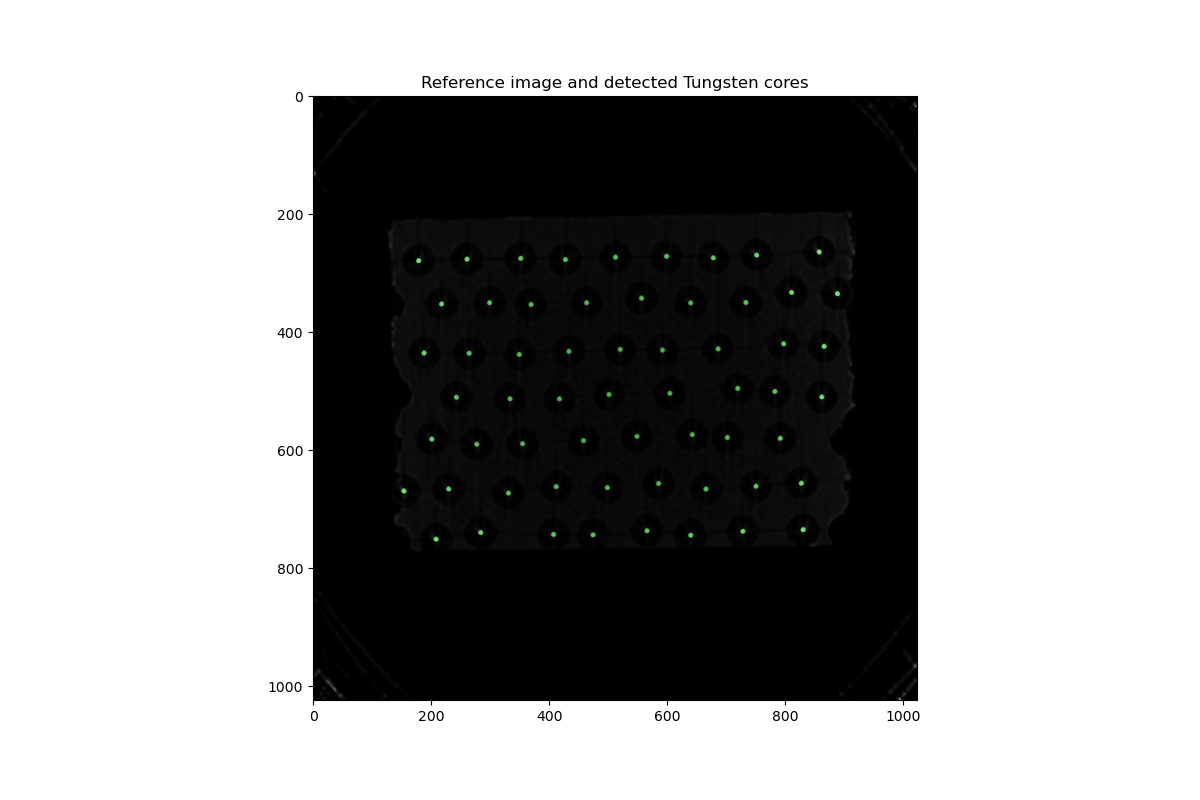
\includegraphics{plots/fibre_detection_using_otsu_method_after_cleaning.png}
\caption{Reference image and detected Tungsten cores using the Otsu's
method after mathematical morphology}
\end{figure}

\hypertarget{mark-each-potential-tungsten-corewith-unique-label}{%
\section{Mark each potential tungsten corewith unique
label}\label{mark-each-potential-tungsten-corewith-unique-label}}

    Each distinct tungsten core is assigned a unique label, i.e.~a unique
pixel intensity

    \begin{tcolorbox}[breakable, size=fbox, boxrule=1pt, pad at break*=1mm,colback=cellbackground, colframe=cellborder]
\prompt{In}{incolor}{36}{\boxspacing}
\begin{Verbatim}[commandchars=\\\{\}]
\PY{n}{core\PYZus{}labels} \PY{o}{=} \PY{n}{sitk}\PY{o}{.}\PY{n}{ConnectedComponent}\PY{p}{(}\PY{n}{cleaned\PYZus{}thresh\PYZus{}img}\PY{p}{)}\PY{p}{;}
\end{Verbatim}
\end{tcolorbox}

    \begin{tcolorbox}[breakable, size=fbox, boxrule=1pt, pad at break*=1mm,colback=cellbackground, colframe=cellborder]
\prompt{In}{incolor}{37}{\boxspacing}
\begin{Verbatim}[commandchars=\\\{\}]
\PY{n}{fig} \PY{o}{=} \PY{n}{plt}\PY{o}{.}\PY{n}{figure}\PY{p}{(}\PY{p}{)}\PY{p}{;}
\PY{n}{imgplot} \PY{o}{=} \PY{n}{plt}\PY{o}{.}\PY{n}{imshow}\PY{p}{(}\PY{n}{sitk}\PY{o}{.}\PY{n}{GetArrayViewFromImage}\PY{p}{(}\PY{n}{sitk}\PY{o}{.}\PY{n}{LabelOverlay}\PY{p}{(}\PY{n}{volume}\PY{p}{,} \PY{n}{core\PYZus{}labels}\PY{p}{)}\PY{p}{)}\PY{p}{)}\PY{p}{;}
\PY{n}{plt}\PY{o}{.}\PY{n}{title}\PY{p}{(}\PY{l+s+s2}{\PYZdq{}}\PY{l+s+s2}{Cleaned Binary Segmentation of the Tungsten cores}\PY{l+s+s2}{\PYZdq{}}\PY{p}{)}\PY{p}{;}
\PY{n}{plt}\PY{o}{.}\PY{n}{savefig}\PY{p}{(}\PY{l+s+s1}{\PYZsq{}}\PY{l+s+s1}{plots/fibre\PYZus{}detection\PYZus{}with\PYZus{}label\PYZus{}overlay.pdf}\PY{l+s+s1}{\PYZsq{}}\PY{p}{)}\PY{p}{;}
\PY{n}{plt}\PY{o}{.}\PY{n}{savefig}\PY{p}{(}\PY{l+s+s1}{\PYZsq{}}\PY{l+s+s1}{plots/fibre\PYZus{}detection\PYZus{}with\PYZus{}label\PYZus{}overlay.png}\PY{l+s+s1}{\PYZsq{}}\PY{p}{)}\PY{p}{;}
\end{Verbatim}
\end{tcolorbox}

    \begin{figure}
\centering
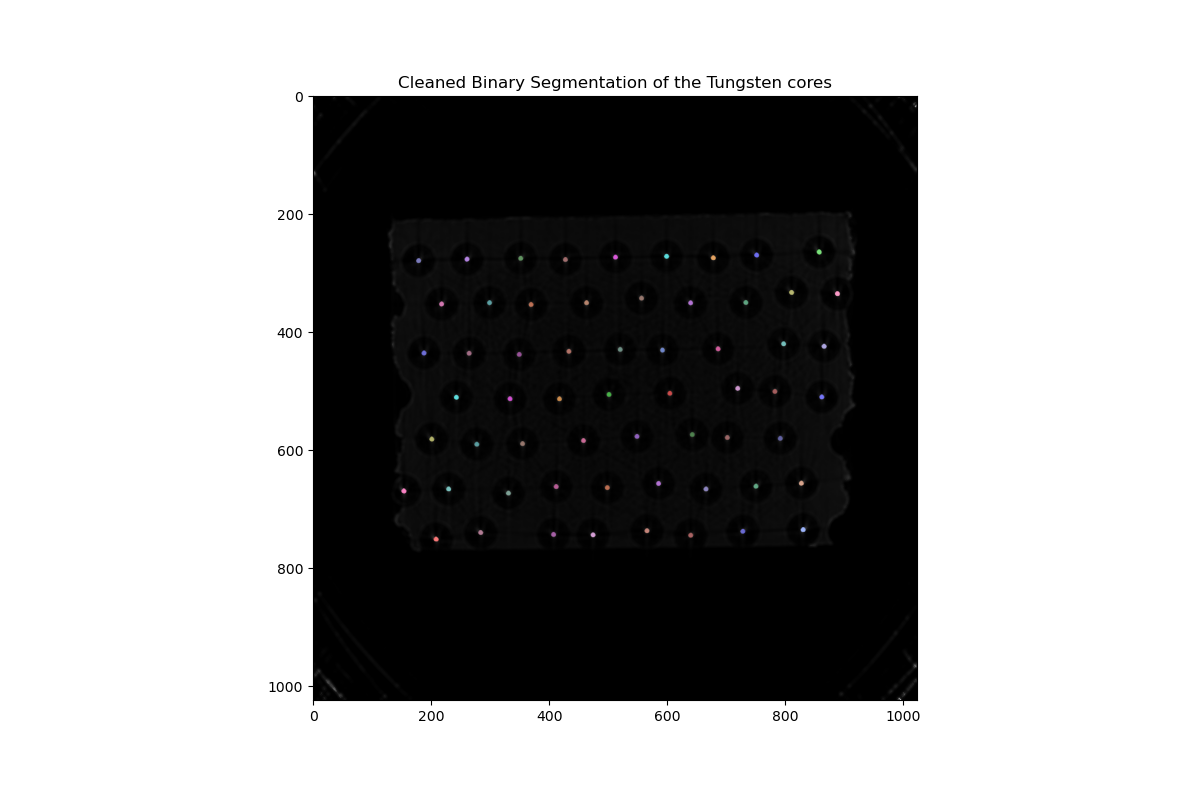
\includegraphics{plots/fibre_detection_with_label_overlay.png}
\caption{Reference image and labelled detected Tungsten cores}
\end{figure}

\hypertarget{object-analysis}{%
\subsection{Object Analysis}\label{object-analysis}}

    Once we have the segmented objects we look at their shapes and the
intensity distributions inside the objects. For each labelled tungsten
core, we extract the centroid. Note that sizes and positions are given
in millimetres.

    \begin{tcolorbox}[breakable, size=fbox, boxrule=1pt, pad at break*=1mm,colback=cellbackground, colframe=cellborder]
\prompt{In}{incolor}{38}{\boxspacing}
\begin{Verbatim}[commandchars=\\\{\}]
\PY{n}{shape\PYZus{}stats} \PY{o}{=} \PY{n}{sitk}\PY{o}{.}\PY{n}{LabelShapeStatisticsImageFilter}\PY{p}{(}\PY{p}{)}
\PY{n}{shape\PYZus{}stats}\PY{o}{.}\PY{n}{ComputeOrientedBoundingBoxOn}\PY{p}{(}\PY{p}{)}
\PY{n}{shape\PYZus{}stats}\PY{o}{.}\PY{n}{Execute}\PY{p}{(}\PY{n}{core\PYZus{}labels}\PY{p}{)}
\end{Verbatim}
\end{tcolorbox}

    \begin{tcolorbox}[breakable, size=fbox, boxrule=1pt, pad at break*=1mm,colback=cellbackground, colframe=cellborder]
\prompt{In}{incolor}{39}{\boxspacing}
\begin{Verbatim}[commandchars=\\\{\}]
\PY{n}{centroid\PYZus{}set} \PY{o}{=} \PY{p}{[}\PY{p}{]}\PY{p}{;}

\PY{k}{for} \PY{n}{i} \PY{o+ow}{in} \PY{n}{shape\PYZus{}stats}\PY{o}{.}\PY{n}{GetLabels}\PY{p}{(}\PY{p}{)}\PY{p}{:}
    \PY{n}{centroid\PYZus{}set}\PY{o}{.}\PY{n}{append}\PY{p}{(}\PY{n}{cleaned\PYZus{}thresh\PYZus{}img}\PY{o}{.}\PY{n}{TransformPhysicalPointToIndex}\PY{p}{(}\PY{n}{shape\PYZus{}stats}\PY{o}{.}\PY{n}{GetCentroid}\PY{p}{(}\PY{n}{i}\PY{p}{)}\PY{p}{)}\PY{p}{)}\PY{p}{;}
\end{Verbatim}
\end{tcolorbox}

    We now have a list of the centres of all the fibres that can be used as
a parameter of the function below to create the cylinders corresponding
to the cores and the fibres. For each core, a cylinder is creatd and
translated:

\begin{Shaded}
\begin{Highlighting}[]
\NormalTok{        gvxr.emptyMesh(}\StringTok{"core\_"}  \OperatorTok{+} \BuiltInTok{str}\NormalTok{(i))}\OperatorTok{;}
\NormalTok{        gvxr.makeCylinder(}\StringTok{"core\_"}  \OperatorTok{+} \BuiltInTok{str}\NormalTok{(i), number\_of\_sectors, }\FloatTok{815.0}\NormalTok{,  core\_radius, }\StringTok{"micrometer"}\NormalTok{)}\OperatorTok{;}
\NormalTok{        gvxr.translateNode(}\StringTok{"core\_"}  \OperatorTok{+} \BuiltInTok{str}\NormalTok{(i), y, }\FloatTok{0.0}\NormalTok{, x, }\StringTok{"micrometer"}\NormalTok{)}\OperatorTok{;}
\end{Highlighting}
\end{Shaded}

For each fibre, another cylinder is created and translated:

\begin{Shaded}
\begin{Highlighting}[]
\NormalTok{        gvxr.emptyMesh(}\StringTok{"fibre\_"}  \OperatorTok{+} \BuiltInTok{str}\NormalTok{(i))}\OperatorTok{;}
\NormalTok{        gvxr.makeCylinder(}\StringTok{"fibre\_"}  \OperatorTok{+} \BuiltInTok{str}\NormalTok{(i), number\_of\_sectors, }\FloatTok{815.0}\NormalTok{,  fibre\_radius, }\StringTok{"micrometer"}\NormalTok{)}\OperatorTok{;}
\NormalTok{        gvxr.translateNode(}\StringTok{"fibre\_"}  \OperatorTok{+} \BuiltInTok{str}\NormalTok{(i), y, }\FloatTok{0.0}\NormalTok{, x, }\StringTok{"micrometer"}\NormalTok{)}\OperatorTok{;}
\end{Highlighting}
\end{Shaded}

The fibre's cylinder is hollowed to make space for its core:

\begin{Shaded}
\begin{Highlighting}[]
\NormalTok{        gvxr.subtractMesh(}\StringTok{"fibre\_"} \OperatorTok{+} \BuiltInTok{str}\NormalTok{(i), }\StringTok{"core\_"} \OperatorTok{+} \BuiltInTok{str}\NormalTok{(i))}\OperatorTok{;}
\end{Highlighting}
\end{Shaded}

    \begin{tcolorbox}[breakable, size=fbox, boxrule=1pt, pad at break*=1mm,colback=cellbackground, colframe=cellborder]
\prompt{In}{incolor}{40}{\boxspacing}
\begin{Verbatim}[commandchars=\\\{\}]
\PY{k}{def} \PY{n+nf}{setFibres}\PY{p}{(}\PY{n}{aCentroidSet}\PY{p}{)}\PY{p}{:}
    \PY{l+s+sd}{\PYZdq{}\PYZdq{}\PYZdq{}This function loads a cylinders in the GPU memory.}
\PY{l+s+sd}{    Some are hollow and represent the fibres, some are not and}
\PY{l+s+sd}{    correspond to the cores.}

\PY{l+s+sd}{    :param array aCentroidSet: a list of cylinder centres.}
\PY{l+s+sd}{    \PYZdq{}\PYZdq{}\PYZdq{}}

    \PY{k}{global} \PY{n}{core\PYZus{}radius}\PY{p}{;}
    \PY{k}{global} \PY{n}{fibre\PYZus{}radius}\PY{p}{;}

    \PY{c+c1}{\PYZsh{} Create empty geometries}
    \PY{n}{gvxr}\PY{o}{.}\PY{n}{emptyMesh}\PY{p}{(}\PY{l+s+s2}{\PYZdq{}}\PY{l+s+s2}{fibre}\PY{l+s+s2}{\PYZdq{}}\PY{p}{)}\PY{p}{;}
    \PY{n}{gvxr}\PY{o}{.}\PY{n}{emptyMesh}\PY{p}{(}\PY{l+s+s2}{\PYZdq{}}\PY{l+s+s2}{core}\PY{l+s+s2}{\PYZdq{}}\PY{p}{)}\PY{p}{;}

    \PY{c+c1}{\PYZsh{} Number of sectors to approximate cylinders with triangle meshes}
    \PY{c+c1}{\PYZsh{} It controls the accuracy of the meshes.}
    \PY{n}{number\PYZus{}of\PYZus{}sectors} \PY{o}{=} \PY{l+m+mi}{100}\PY{p}{;}

    \PY{c+c1}{\PYZsh{} Process all the centres from the input list}
    \PY{k}{for} \PY{n}{i}\PY{p}{,} \PY{n}{cyl} \PY{o+ow}{in} \PY{n+nb}{enumerate}\PY{p}{(}\PY{n}{aCentroidSet}\PY{p}{)}\PY{p}{:}

        \PY{c+c1}{\PYZsh{} Convert the centre position from 2D image coordinates in 3D world coordinates}
        \PY{n}{x} \PY{o}{=} \PY{n}{pixel\PYZus{}spacing\PYZus{}in\PYZus{}micrometre} \PY{o}{*} \PY{o}{\PYZhy{}}\PY{p}{(}\PY{n}{cyl}\PY{p}{[}\PY{l+m+mi}{0}\PY{p}{]} \PY{o}{\PYZhy{}} \PY{n}{reference\PYZus{}CT}\PY{o}{.}\PY{n}{shape}\PY{p}{[}\PY{l+m+mi}{1}\PY{p}{]} \PY{o}{/} \PY{l+m+mi}{2} \PY{o}{+} \PY{l+m+mf}{0.5}\PY{p}{)}\PY{p}{;}
        \PY{n}{y} \PY{o}{=} \PY{n}{pixel\PYZus{}spacing\PYZus{}in\PYZus{}micrometre} \PY{o}{*} \PY{p}{(}\PY{n}{cyl}\PY{p}{[}\PY{l+m+mi}{1}\PY{p}{]} \PY{o}{\PYZhy{}} \PY{n}{reference\PYZus{}CT}\PY{o}{.}\PY{n}{shape}\PY{p}{[}\PY{l+m+mi}{0}\PY{p}{]} \PY{o}{/} \PY{l+m+mi}{2} \PY{o}{+} \PY{l+m+mf}{0.5}\PY{p}{)}\PY{p}{;}

        \PY{c+c1}{\PYZsh{} Create empty geometries (is it needed?)}
        \PY{n}{gvxr}\PY{o}{.}\PY{n}{emptyMesh}\PY{p}{(}\PY{l+s+s2}{\PYZdq{}}\PY{l+s+s2}{fibre\PYZus{}}\PY{l+s+s2}{\PYZdq{}} \PY{o}{+} \PY{n+nb}{str}\PY{p}{(}\PY{n}{i}\PY{p}{)}\PY{p}{)}\PY{p}{;}
        \PY{n}{gvxr}\PY{o}{.}\PY{n}{emptyMesh}\PY{p}{(}\PY{l+s+s2}{\PYZdq{}}\PY{l+s+s2}{core\PYZus{}}\PY{l+s+s2}{\PYZdq{}} \PY{o}{+} \PY{n+nb}{str}\PY{p}{(}\PY{n}{i}\PY{p}{)}\PY{p}{)}\PY{p}{;}

        \PY{c+c1}{\PYZsh{} Create the two corresponding cylinders (fibre and core)}
        \PY{n}{gvxr}\PY{o}{.}\PY{n}{makeCylinder}\PY{p}{(}\PY{l+s+s2}{\PYZdq{}}\PY{l+s+s2}{fibre\PYZus{}}\PY{l+s+s2}{\PYZdq{}} \PY{o}{+} \PY{n+nb}{str}\PY{p}{(}\PY{n}{i}\PY{p}{)}\PY{p}{,} \PY{n}{number\PYZus{}of\PYZus{}sectors}\PY{p}{,} \PY{l+m+mf}{815.0}\PY{p}{,} \PY{n}{fibre\PYZus{}radius}\PY{p}{,} \PY{l+s+s2}{\PYZdq{}}\PY{l+s+s2}{micrometer}\PY{l+s+s2}{\PYZdq{}}\PY{p}{)}\PY{p}{;}
        \PY{n}{gvxr}\PY{o}{.}\PY{n}{makeCylinder}\PY{p}{(}\PY{l+s+s2}{\PYZdq{}}\PY{l+s+s2}{core\PYZus{}}\PY{l+s+s2}{\PYZdq{}}  \PY{o}{+} \PY{n+nb}{str}\PY{p}{(}\PY{n}{i}\PY{p}{)}\PY{p}{,} \PY{n}{number\PYZus{}of\PYZus{}sectors}\PY{p}{,} \PY{l+m+mf}{815.0}\PY{p}{,}  \PY{n}{core\PYZus{}radius}\PY{p}{,} \PY{l+s+s2}{\PYZdq{}}\PY{l+s+s2}{micrometer}\PY{l+s+s2}{\PYZdq{}}\PY{p}{)}\PY{p}{;}

        \PY{c+c1}{\PYZsh{} Translate the two cylinders to the position of their centre}
        \PY{n}{gvxr}\PY{o}{.}\PY{n}{translateNode}\PY{p}{(}\PY{l+s+s2}{\PYZdq{}}\PY{l+s+s2}{fibre\PYZus{}}\PY{l+s+s2}{\PYZdq{}} \PY{o}{+} \PY{n+nb}{str}\PY{p}{(}\PY{n}{i}\PY{p}{)}\PY{p}{,} \PY{n}{y}\PY{p}{,} \PY{l+m+mf}{0.0}\PY{p}{,} \PY{n}{x}\PY{p}{,} \PY{l+s+s2}{\PYZdq{}}\PY{l+s+s2}{micrometer}\PY{l+s+s2}{\PYZdq{}}\PY{p}{)}\PY{p}{;}
        \PY{n}{gvxr}\PY{o}{.}\PY{n}{translateNode}\PY{p}{(}\PY{l+s+s2}{\PYZdq{}}\PY{l+s+s2}{core\PYZus{}}\PY{l+s+s2}{\PYZdq{}} \PY{o}{+} \PY{n+nb}{str}\PY{p}{(}\PY{n}{i}\PY{p}{)}\PY{p}{,} \PY{n}{y}\PY{p}{,} \PY{l+m+mf}{0.0}\PY{p}{,} \PY{n}{x}\PY{p}{,} \PY{l+s+s2}{\PYZdq{}}\PY{l+s+s2}{micrometer}\PY{l+s+s2}{\PYZdq{}}\PY{p}{)}\PY{p}{;}

        \PY{c+c1}{\PYZsh{} Apply the local transformation matrix (so that we could save the corresponding STL files)}
        \PY{n}{gvxr}\PY{o}{.}\PY{n}{applyCurrentLocalTransformation}\PY{p}{(}\PY{l+s+s2}{\PYZdq{}}\PY{l+s+s2}{fibre\PYZus{}}\PY{l+s+s2}{\PYZdq{}} \PY{o}{+} \PY{n+nb}{str}\PY{p}{(}\PY{n}{i}\PY{p}{)}\PY{p}{)}\PY{p}{;}
        \PY{n}{gvxr}\PY{o}{.}\PY{n}{applyCurrentLocalTransformation}\PY{p}{(}\PY{l+s+s2}{\PYZdq{}}\PY{l+s+s2}{core\PYZus{}}\PY{l+s+s2}{\PYZdq{}} \PY{o}{+} \PY{n+nb}{str}\PY{p}{(}\PY{n}{i}\PY{p}{)}\PY{p}{)}\PY{p}{;}

        \PY{c+c1}{\PYZsh{} Subtract the fibre from the matrix}
        \PY{n}{gvxr}\PY{o}{.}\PY{n}{subtractMesh}\PY{p}{(}\PY{l+s+s2}{\PYZdq{}}\PY{l+s+s2}{matrix}\PY{l+s+s2}{\PYZdq{}}\PY{p}{,} \PY{l+s+s2}{\PYZdq{}}\PY{l+s+s2}{fibre\PYZus{}}\PY{l+s+s2}{\PYZdq{}} \PY{o}{+} \PY{n+nb}{str}\PY{p}{(}\PY{n}{i}\PY{p}{)}\PY{p}{)}\PY{p}{;}

        \PY{c+c1}{\PYZsh{} Subtract the core from the fibre}
        \PY{n}{gvxr}\PY{o}{.}\PY{n}{subtractMesh}\PY{p}{(}\PY{l+s+s2}{\PYZdq{}}\PY{l+s+s2}{fibre\PYZus{}}\PY{l+s+s2}{\PYZdq{}} \PY{o}{+} \PY{n+nb}{str}\PY{p}{(}\PY{n}{i}\PY{p}{)}\PY{p}{,} \PY{l+s+s2}{\PYZdq{}}\PY{l+s+s2}{core\PYZus{}}\PY{l+s+s2}{\PYZdq{}} \PY{o}{+} \PY{n+nb}{str}\PY{p}{(}\PY{n}{i}\PY{p}{)}\PY{p}{)}\PY{p}{;}

        \PY{c+c1}{\PYZsh{} Save the corresponding STL files}
        \PY{c+c1}{\PYZsh{} gvxr.saveSTLfile(\PYZdq{}fibre\PYZus{}\PYZdq{} + str(i), \PYZdq{}Tutorial2/outputs/fibre\PYZus{}\PYZdq{} + str(i) + \PYZdq{}.stl\PYZdq{});}
        \PY{c+c1}{\PYZsh{} gvxr.saveSTLfile(\PYZdq{}core\PYZus{}\PYZdq{} + str(i),  \PYZdq{}Tutorial2/outputs/core\PYZus{}\PYZdq{}  + str(i) + \PYZdq{}.stl\PYZdq{});}

        \PY{c+c1}{\PYZsh{} Add the mesh of the current fibre to the overall fibre mesh}
        \PY{n}{gvxr}\PY{o}{.}\PY{n}{addMesh}\PY{p}{(}\PY{l+s+s2}{\PYZdq{}}\PY{l+s+s2}{fibre}\PY{l+s+s2}{\PYZdq{}}\PY{p}{,} \PY{l+s+s2}{\PYZdq{}}\PY{l+s+s2}{fibre\PYZus{}}\PY{l+s+s2}{\PYZdq{}} \PY{o}{+} \PY{n+nb}{str}\PY{p}{(}\PY{n}{i}\PY{p}{)}\PY{p}{)}\PY{p}{;}

        \PY{c+c1}{\PYZsh{} Add the mesh of the current core to the overall core mesh}
        \PY{n}{gvxr}\PY{o}{.}\PY{n}{addMesh}\PY{p}{(}\PY{l+s+s2}{\PYZdq{}}\PY{l+s+s2}{core}\PY{l+s+s2}{\PYZdq{}}\PY{p}{,} \PY{l+s+s2}{\PYZdq{}}\PY{l+s+s2}{core\PYZus{}}\PY{l+s+s2}{\PYZdq{}}  \PY{o}{+} \PY{n+nb}{str}\PY{p}{(}\PY{n}{i}\PY{p}{)}\PY{p}{)}\PY{p}{;}

    \PY{c+c1}{\PYZsh{} Set the mesh colours (for the interactive visualisation)}
    \PY{n}{gvxr}\PY{o}{.}\PY{n}{setColor}\PY{p}{(}\PY{l+s+s2}{\PYZdq{}}\PY{l+s+s2}{fibre}\PY{l+s+s2}{\PYZdq{}}\PY{p}{,} \PY{l+m+mf}{1.0}\PY{p}{,} \PY{l+m+mf}{0.0}\PY{p}{,} \PY{l+m+mf}{0.0}\PY{p}{,} \PY{l+m+mf}{1.0}\PY{p}{)}\PY{p}{;}
    \PY{n}{gvxr}\PY{o}{.}\PY{n}{setColor}\PY{p}{(}\PY{l+s+s2}{\PYZdq{}}\PY{l+s+s2}{core}\PY{l+s+s2}{\PYZdq{}}\PY{p}{,}  \PY{l+m+mf}{1.0}\PY{p}{,} \PY{l+m+mf}{0.0}\PY{p}{,} \PY{l+m+mf}{1.0}\PY{p}{,} \PY{l+m+mf}{1.0}\PY{p}{)}\PY{p}{;}

    \PY{c+c1}{\PYZsh{} Set the fibre\PYZsq{}s material properties}
    \PY{c+c1}{\PYZsh{} gvxr.setLinearAttenuationCoefficient(\PYZdq{}fibre\PYZdq{}, fibre\PYZus{}mu, \PYZdq{}cm\PYZhy{}1\PYZdq{});}
    \PY{n}{gvxr}\PY{o}{.}\PY{n}{setCompound}\PY{p}{(}\PY{l+s+s2}{\PYZdq{}}\PY{l+s+s2}{fibre}\PY{l+s+s2}{\PYZdq{}}\PY{p}{,} \PY{l+s+s2}{\PYZdq{}}\PY{l+s+s2}{SiC}\PY{l+s+s2}{\PYZdq{}}\PY{p}{)}\PY{p}{;}
    \PY{n}{gvxr}\PY{o}{.}\PY{n}{setDensity}\PY{p}{(}\PY{l+s+s2}{\PYZdq{}}\PY{l+s+s2}{fibre}\PY{l+s+s2}{\PYZdq{}}\PY{p}{,} \PY{n}{fibre\PYZus{}density}\PY{p}{,} \PY{l+s+s2}{\PYZdq{}}\PY{l+s+s2}{g/cm3}\PY{l+s+s2}{\PYZdq{}}\PY{p}{)}\PY{p}{;}

    \PY{c+c1}{\PYZsh{} Set the core\PYZsq{}s material properties}
    \PY{c+c1}{\PYZsh{} gvxr.setLinearAttenuationCoefficient(\PYZdq{}core\PYZdq{}, core\PYZus{}mu, \PYZdq{}cm\PYZhy{}1\PYZdq{});}
    \PY{n}{gvxr}\PY{o}{.}\PY{n}{setElement}\PY{p}{(}\PY{l+s+s2}{\PYZdq{}}\PY{l+s+s2}{core}\PY{l+s+s2}{\PYZdq{}}\PY{p}{,} \PY{l+s+s2}{\PYZdq{}}\PY{l+s+s2}{W}\PY{l+s+s2}{\PYZdq{}}\PY{p}{)}\PY{p}{;}

    \PY{c+c1}{\PYZsh{} Add the fibres and cores to the X\PYZhy{}ray renderer}
    \PY{n}{gvxr}\PY{o}{.}\PY{n}{addPolygonMeshAsInnerSurface}\PY{p}{(}\PY{l+s+s2}{\PYZdq{}}\PY{l+s+s2}{core}\PY{l+s+s2}{\PYZdq{}}\PY{p}{)}\PY{p}{;}
    \PY{n}{gvxr}\PY{o}{.}\PY{n}{addPolygonMeshAsInnerSurface}\PY{p}{(}\PY{l+s+s2}{\PYZdq{}}\PY{l+s+s2}{fibre}\PY{l+s+s2}{\PYZdq{}}\PY{p}{)}\PY{p}{;}
\end{Verbatim}
\end{tcolorbox}

    \hypertarget{registration-of-a-cube}{%
\section{Registration of a cube}\label{registration-of-a-cube}}

    We define a function to create the polygon mesh of the Ti90Al6V4 matrix.

    \begin{tcolorbox}[breakable, size=fbox, boxrule=1pt, pad at break*=1mm,colback=cellbackground, colframe=cellborder]
\prompt{In}{incolor}{41}{\boxspacing}
\begin{Verbatim}[commandchars=\\\{\}]
\PY{k}{def} \PY{n+nf}{setMatrix}\PY{p}{(}\PY{n}{apGeneSet}\PY{p}{)}\PY{p}{:}
    \PY{l+s+sd}{\PYZdq{}\PYZdq{}\PYZdq{}This function loads a cube in the GPU memory. The cube represents}
\PY{l+s+sd}{    the Ti90Al6V4 matrix.}

\PY{l+s+sd}{    apGeneSet[0] is a number between \PYZhy{}0.5 and 0.5, related to the translation vector (X component) of the cube. It can be interpreted as a percentage of the detector width.}
\PY{l+s+sd}{    apGeneSet[1] is the same as apGeneSet[0], but related to the Y component of the translation vector.}
\PY{l+s+sd}{    apGeneSet[2] is a number between \PYZhy{}0.5 and 0.5, related to the rotation angle in degrees}
\PY{l+s+sd}{    apGeneSet[3] is a scaling factor between \PYZhy{}0.5 and 0.5. It can be interpreted as a percentage of the detector width.}
\PY{l+s+sd}{    apGeneSet[4] is a scaling factor between \PYZhy{}0.5 and 0.5. It can be interpreted as a percentage of apGeneSet[3].}
\PY{l+s+sd}{    \PYZdq{}\PYZdq{}\PYZdq{}}

    \PY{c+c1}{\PYZsh{} Remove all the geometries from the whole scenegraph}
    \PY{n}{gvxr}\PY{o}{.}\PY{n}{removePolygonMeshesFromSceneGraph}\PY{p}{(}\PY{p}{)}\PY{p}{;}

    \PY{c+c1}{\PYZsh{} Make a cube}
    \PY{n}{gvxr}\PY{o}{.}\PY{n}{makeCube}\PY{p}{(}\PY{l+s+s2}{\PYZdq{}}\PY{l+s+s2}{matrix}\PY{l+s+s2}{\PYZdq{}}\PY{p}{,} \PY{l+m+mf}{1.0}\PY{p}{,} \PY{l+s+s2}{\PYZdq{}}\PY{l+s+s2}{micrometer}\PY{l+s+s2}{\PYZdq{}}\PY{p}{)}\PY{p}{;}

    \PY{c+c1}{\PYZsh{} Translation vector}
    \PY{n}{x} \PY{o}{=} \PY{n}{apGeneSet}\PY{p}{[}\PY{l+m+mi}{0}\PY{p}{]} \PY{o}{*} \PY{n}{detector\PYZus{}width\PYZus{}in\PYZus{}pixels} \PY{o}{*} \PY{n}{pixel\PYZus{}spacing\PYZus{}in\PYZus{}micrometre}\PY{p}{;}
    \PY{n}{y} \PY{o}{=} \PY{n}{apGeneSet}\PY{p}{[}\PY{l+m+mi}{1}\PY{p}{]} \PY{o}{*} \PY{n}{detector\PYZus{}width\PYZus{}in\PYZus{}pixels} \PY{o}{*} \PY{n}{pixel\PYZus{}spacing\PYZus{}in\PYZus{}micrometre}\PY{p}{;}
    \PY{n}{gvxr}\PY{o}{.}\PY{n}{translateNode}\PY{p}{(}\PY{l+s+s2}{\PYZdq{}}\PY{l+s+s2}{matrix}\PY{l+s+s2}{\PYZdq{}}\PY{p}{,} \PY{n}{x}\PY{p}{,} \PY{l+m+mf}{0.0}\PY{p}{,} \PY{n}{y}\PY{p}{,} \PY{l+s+s2}{\PYZdq{}}\PY{l+s+s2}{micrometer}\PY{l+s+s2}{\PYZdq{}}\PY{p}{)}\PY{p}{;}

    \PY{c+c1}{\PYZsh{} Rotation angle}
    \PY{n}{rotation\PYZus{}angle\PYZus{}in\PYZus{}degrees} \PY{o}{=} \PY{p}{(}\PY{n}{apGeneSet}\PY{p}{[}\PY{l+m+mi}{2}\PY{p}{]} \PY{o}{+} \PY{l+m+mf}{0.5}\PY{p}{)} \PY{o}{*} \PY{l+m+mf}{180.0}\PY{p}{;}
    \PY{n}{gvxr}\PY{o}{.}\PY{n}{rotateNode}\PY{p}{(}\PY{l+s+s2}{\PYZdq{}}\PY{l+s+s2}{matrix}\PY{l+s+s2}{\PYZdq{}}\PY{p}{,} \PY{n}{rotation\PYZus{}angle\PYZus{}in\PYZus{}degrees}\PY{p}{,} \PY{l+m+mi}{0}\PY{p}{,} \PY{l+m+mi}{1}\PY{p}{,} \PY{l+m+mi}{0}\PY{p}{)}\PY{p}{;}

    \PY{c+c1}{\PYZsh{} Scaling factors}
    \PY{n}{w} \PY{o}{=} \PY{p}{(}\PY{n}{apGeneSet}\PY{p}{[}\PY{l+m+mi}{3}\PY{p}{]} \PY{o}{+} \PY{l+m+mf}{0.5}\PY{p}{)} \PY{o}{*} \PY{n}{detector\PYZus{}width\PYZus{}in\PYZus{}pixels} \PY{o}{*} \PY{n}{pixel\PYZus{}spacing\PYZus{}in\PYZus{}micrometre}\PY{p}{;}
    \PY{n}{h} \PY{o}{=} \PY{p}{(}\PY{n}{apGeneSet}\PY{p}{[}\PY{l+m+mi}{4}\PY{p}{]} \PY{o}{+} \PY{l+m+mf}{0.5}\PY{p}{)} \PY{o}{*} \PY{n}{w}\PY{p}{;}
    \PY{n}{gvxr}\PY{o}{.}\PY{n}{scaleNode}\PY{p}{(}\PY{l+s+s2}{\PYZdq{}}\PY{l+s+s2}{matrix}\PY{l+s+s2}{\PYZdq{}}\PY{p}{,} \PY{n}{w}\PY{p}{,} \PY{l+m+mi}{815}\PY{p}{,} \PY{n}{h}\PY{p}{)}\PY{p}{;}

    \PY{c+c1}{\PYZsh{} Apply the transformation matrix so that we can save the corresponding STL file}
    \PY{n}{gvxr}\PY{o}{.}\PY{n}{applyCurrentLocalTransformation}\PY{p}{(}\PY{l+s+s2}{\PYZdq{}}\PY{l+s+s2}{matrix}\PY{l+s+s2}{\PYZdq{}}\PY{p}{)}\PY{p}{;}

    \PY{c+c1}{\PYZsh{} Set the matrix\PYZsq{}s material properties}
    \PY{n}{gvxr}\PY{o}{.}\PY{n}{setMixture}\PY{p}{(}\PY{l+s+s2}{\PYZdq{}}\PY{l+s+s2}{matrix}\PY{l+s+s2}{\PYZdq{}}\PY{p}{,} \PY{l+s+s2}{\PYZdq{}}\PY{l+s+s2}{Ti90Al6V4}\PY{l+s+s2}{\PYZdq{}}\PY{p}{)}\PY{p}{;}
    \PY{n}{gvxr}\PY{o}{.}\PY{n}{setDensity}\PY{p}{(}\PY{l+s+s2}{\PYZdq{}}\PY{l+s+s2}{matrix}\PY{l+s+s2}{\PYZdq{}}\PY{p}{,} \PY{n}{matrix\PYZus{}density}\PY{p}{,} \PY{l+s+s2}{\PYZdq{}}\PY{l+s+s2}{g/cm3}\PY{l+s+s2}{\PYZdq{}}\PY{p}{)}\PY{p}{;}

    \PY{c+c1}{\PYZsh{} Add the matrix to the X\PYZhy{}ray renderer}
    \PY{n}{gvxr}\PY{o}{.}\PY{n}{addPolygonMeshAsInnerSurface}\PY{p}{(}\PY{l+s+s2}{\PYZdq{}}\PY{l+s+s2}{matrix}\PY{l+s+s2}{\PYZdq{}}\PY{p}{)}\PY{p}{;}
\end{Verbatim}
\end{tcolorbox}

    \hypertarget{simulate-the-ct-acquisition}{%
\subsection{Simulate the CT
acquisition}\label{simulate-the-ct-acquisition}}

There are 7 successive steps to simulate the XCT data acquisition:

\begin{enumerate}
\def\labelenumi{\arabic{enumi}.}
\tightlist
\item
  Set the fibre and cores geometries and material properties (Step 39)
\item
  Set the matrix geometry and material properties (Step 40)
\item
  Simulate the raw projections for each angle:

  \begin{itemize}
  \tightlist
  \item
    Without phase contrast (Line 5 of Step 45), or
  \item
    With phase contrast (Lines 14-55 of Step 45)
  \end{itemize}
\item
  Apply the LSF (Lines 57-60 of Step 45)
\item
  Apply the flat-field correction (Step 62)
\item
  Add Poison noise (Step\textasciitilde{}\ref{??})
\item
  Apply the minus log normalisation to compute the sinogram (Step 63)
\end{enumerate}

Compute the raw projections and save the data. For this purpose, we
define a new function.

    \begin{tcolorbox}[breakable, size=fbox, boxrule=1pt, pad at break*=1mm,colback=cellbackground, colframe=cellborder]
\prompt{In}{incolor}{42}{\boxspacing}
\begin{Verbatim}[commandchars=\\\{\}]
\PY{k}{def} \PY{n+nf}{tomographyAcquisition}\PY{p}{(}\PY{p}{)}\PY{p}{:}
    \PY{l+s+sd}{\PYZdq{}\PYZdq{}\PYZdq{}}
\PY{l+s+sd}{    This function simulate a CT acquisition.}

\PY{l+s+sd}{    :return the raw projections in keV}
\PY{l+s+sd}{    \PYZdq{}\PYZdq{}\PYZdq{}}

    \PY{c+c1}{\PYZsh{} Crete a new array to save every projection in default unit of energy}
    \PY{n}{raw\PYZus{}projections} \PY{o}{=} \PY{p}{[}\PY{p}{]}\PY{p}{;}

    \PY{c+c1}{\PYZsh{} For each angle, simulate a projection}
    \PY{k}{for} \PY{n}{angle\PYZus{}id} \PY{o+ow}{in} \PY{n+nb}{range}\PY{p}{(}\PY{l+m+mi}{0}\PY{p}{,} \PY{n}{number\PYZus{}of\PYZus{}projections}\PY{p}{)}\PY{p}{:}

        \PY{c+c1}{\PYZsh{} Reset the transformation matrix and rotate the scnned object}
        \PY{n}{gvxr}\PY{o}{.}\PY{n}{resetSceneTransformation}\PY{p}{(}\PY{p}{)}\PY{p}{;}
        \PY{n}{gvxr}\PY{o}{.}\PY{n}{rotateScene}\PY{p}{(}\PY{o}{\PYZhy{}}\PY{n}{angular\PYZus{}step} \PY{o}{*} \PY{n}{angle\PYZus{}id}\PY{p}{,} \PY{l+m+mi}{0}\PY{p}{,} \PY{l+m+mi}{1}\PY{p}{,} \PY{l+m+mi}{0}\PY{p}{)}\PY{p}{;}

        \PY{c+c1}{\PYZsh{} Compute the X\PYZhy{}ray image}
        \PY{n}{xray\PYZus{}image} \PY{o}{=} \PY{n}{np}\PY{o}{.}\PY{n}{array}\PY{p}{(}\PY{n}{gvxr}\PY{o}{.}\PY{n}{computeXRayImage}\PY{p}{(}\PY{p}{)}\PY{p}{)}\PY{p}{;}

        \PY{c+c1}{\PYZsh{} Add the projection}
        \PY{n}{raw\PYZus{}projections}\PY{o}{.}\PY{n}{append}\PY{p}{(}\PY{n}{xray\PYZus{}image}\PY{p}{)}\PY{p}{;}

    \PY{c+c1}{\PYZsh{} Convert from the default unit of energy to keV}
    \PY{n}{raw\PYZus{}projections} \PY{o}{=} \PY{n}{np}\PY{o}{.}\PY{n}{array}\PY{p}{(}\PY{n}{raw\PYZus{}projections}\PY{p}{)}\PY{p}{;}
    \PY{n}{raw\PYZus{}projections\PYZus{}in\PYZus{}keV} \PY{o}{=} \PY{n}{raw\PYZus{}projections} \PY{o}{/} \PY{n}{gvxr}\PY{o}{.}\PY{n}{getUnitOfEnergy}\PY{p}{(}\PY{l+s+s2}{\PYZdq{}}\PY{l+s+s2}{keV}\PY{l+s+s2}{\PYZdq{}}\PY{p}{)}\PY{p}{;}

    \PY{k}{return} \PY{n}{raw\PYZus{}projections\PYZus{}in\PYZus{}keV}\PY{p}{;}
\end{Verbatim}
\end{tcolorbox}

    \hypertarget{flat-filed-correction}{%
\subsection{Flat-filed correction}\label{flat-filed-correction}}

Because the data suffers from a fixed-pattern noise in X-ray imaging in
actual experiments, it is necessary to perform the flat-field correction
of the raw projections using:

\[\mathbf{Proj} = \frac{\mathbf{I} - \mathbf{D}}{\mathbf{F} - \mathbf{D}}\]
\(\mathbf{F}\) (full fields) and \(\mathbf{D}\) (dark fields) are
projection images without sample and acquired with and without the X-ray
beam turned on respectively.

Note that in our example, \texttt{raw\_projections\_in\_keV}
(\(\mathbf{I}\)), \texttt{flat\_field\_image} (\(\mathbf{F}\)) and
\texttt{dark\_field\_image} (\(\mathbf{D}\)) are in keV whereas
\texttt{corrected\_projections} (\(\mathbf{Proj}\)) does not have any
unit:

\[0 \leq \mathbf{I} \leq  \sum_E N_0(E) \times E\\0 \leq \mathbf{Proj} \leq 1\]

We define a new function to compute the flat-field correction.

    \begin{tcolorbox}[breakable, size=fbox, boxrule=1pt, pad at break*=1mm,colback=cellbackground, colframe=cellborder]
\prompt{In}{incolor}{43}{\boxspacing}
\begin{Verbatim}[commandchars=\\\{\}]
\PY{k}{def} \PY{n+nf}{flatFieldCorrection}\PY{p}{(}\PY{n}{raw\PYZus{}projections\PYZus{}in\PYZus{}keV}\PY{p}{)}\PY{p}{:}
    \PY{l+s+sd}{\PYZdq{}\PYZdq{}\PYZdq{}}
\PY{l+s+sd}{    This function applies the flat\PYZhy{}field correction on raw projections.}

\PY{l+s+sd}{    :param 2D\PYZus{}image raw\PYZus{}projections\PYZus{}in\PYZus{}keV: the raw X\PYZhy{}ray projections in keV}
\PY{l+s+sd}{    :return the projections (raw\PYZus{}projections\PYZus{}in\PYZus{}keV) after flat\PYZhy{}field correction}
\PY{l+s+sd}{    \PYZdq{}\PYZdq{}\PYZdq{}}

    \PY{c+c1}{\PYZsh{} Create a mock dark field image}
    \PY{n}{dark\PYZus{}field\PYZus{}image} \PY{o}{=} \PY{n}{np}\PY{o}{.}\PY{n}{zeros}\PY{p}{(}\PY{n}{raw\PYZus{}projections\PYZus{}in\PYZus{}keV}\PY{o}{.}\PY{n}{shape}\PY{p}{)}\PY{p}{;}

    \PY{c+c1}{\PYZsh{} Create a mock flat field image}
    \PY{n}{flat\PYZus{}field\PYZus{}image} \PY{o}{=} \PY{n}{np}\PY{o}{.}\PY{n}{ones}\PY{p}{(}\PY{n}{raw\PYZus{}projections\PYZus{}in\PYZus{}keV}\PY{o}{.}\PY{n}{shape}\PY{p}{)}\PY{p}{;}

    \PY{c+c1}{\PYZsh{} Retrieve the total energy}
    \PY{n}{total\PYZus{}energy} \PY{o}{=} \PY{l+m+mf}{0.0}\PY{p}{;}
    \PY{n}{energy\PYZus{}bins} \PY{o}{=} \PY{n}{gvxr}\PY{o}{.}\PY{n}{getEnergyBins}\PY{p}{(}\PY{l+s+s2}{\PYZdq{}}\PY{l+s+s2}{keV}\PY{l+s+s2}{\PYZdq{}}\PY{p}{)}\PY{p}{;}
    \PY{n}{photon\PYZus{}count\PYZus{}per\PYZus{}bin} \PY{o}{=} \PY{n}{gvxr}\PY{o}{.}\PY{n}{getPhotonCountEnergyBins}\PY{p}{(}\PY{p}{)}\PY{p}{;}

    \PY{k}{for} \PY{n}{energy}\PY{p}{,} \PY{n}{count} \PY{o+ow}{in} \PY{n+nb}{zip}\PY{p}{(}\PY{n}{energy\PYZus{}bins}\PY{p}{,} \PY{n}{photon\PYZus{}count\PYZus{}per\PYZus{}bin}\PY{p}{)}\PY{p}{:}
        \PY{n}{total\PYZus{}energy} \PY{o}{+}\PY{o}{=} \PY{n}{energy} \PY{o}{*} \PY{n}{count}\PY{p}{;}
    \PY{n}{flat\PYZus{}field\PYZus{}image} \PY{o}{*}\PY{o}{=} \PY{n}{total\PYZus{}energy}\PY{p}{;}

    \PY{c+c1}{\PYZsh{} Apply the actual flat\PYZhy{}field correction on the raw projections}
    \PY{n}{corrected\PYZus{}projections} \PY{o}{=} \PY{p}{(}\PY{n}{raw\PYZus{}projections\PYZus{}in\PYZus{}keV} \PY{o}{\PYZhy{}} \PY{n}{dark\PYZus{}field\PYZus{}image}\PY{p}{)} \PY{o}{/} \PY{p}{(}\PY{n}{flat\PYZus{}field\PYZus{}image} \PY{o}{\PYZhy{}} \PY{n}{dark\PYZus{}field\PYZus{}image}\PY{p}{)}\PY{p}{;}

    \PY{k}{return} \PY{n}{corrected\PYZus{}projections}\PY{p}{;}
\end{Verbatim}
\end{tcolorbox}

    The function below is used to simulate a sinogram acquisition. Phase
contrast in the projections can be taken into account or not. Also,
Poisson noise can be added.

    \begin{tcolorbox}[breakable, size=fbox, boxrule=1pt, pad at break*=1mm,colback=cellbackground, colframe=cellborder]
\prompt{In}{incolor}{44}{\boxspacing}
\begin{Verbatim}[commandchars=\\\{\}]
\PY{k}{def} \PY{n+nf}{simulateSinogram}\PY{p}{(}\PY{n}{sigma\PYZus{}set}\PY{o}{=}\PY{k+kc}{None}\PY{p}{,} \PY{n}{k\PYZus{}set}\PY{o}{=}\PY{k+kc}{None}\PY{p}{,} \PY{n}{name\PYZus{}set}\PY{o}{=}\PY{k+kc}{None}\PY{p}{)}\PY{p}{:}

    \PY{k}{global} \PY{n}{lsf\PYZus{}kernel}\PY{p}{;}

    \PY{c+c1}{\PYZsh{} Do not simulate the phase contrast using a Laplacian}
    \PY{k}{if} \PY{n+nb}{isinstance}\PY{p}{(}\PY{n}{sigma\PYZus{}set}\PY{p}{,} \PY{n}{NoneType}\PY{p}{)} \PY{o+ow}{or} \PY{n+nb}{isinstance}\PY{p}{(}\PY{n}{k\PYZus{}set}\PY{p}{,} \PY{n}{NoneType}\PY{p}{)} \PY{o+ow}{or} \PY{n+nb}{isinstance}\PY{p}{(}\PY{n}{name\PYZus{}set}\PY{p}{,} \PY{n}{NoneType}\PY{p}{)}\PY{p}{:}

        \PY{c+c1}{\PYZsh{} Get the raw projections in keV}
        \PY{n}{raw\PYZus{}projections\PYZus{}in\PYZus{}keV} \PY{o}{=} \PY{n}{tomographyAcquisition}\PY{p}{(}\PY{p}{)}\PY{p}{;}

    \PY{c+c1}{\PYZsh{} Simulate the phase contrast using a Laplacian}
    \PY{k}{else}\PY{p}{:}

        \PY{c+c1}{\PYZsh{} Create the convolution filter}
        \PY{n}{pixel\PYZus{}range} \PY{o}{=} \PY{n}{np}\PY{o}{.}\PY{n}{linspace}\PY{p}{(}\PY{o}{\PYZhy{}}\PY{n}{value\PYZus{}range}\PY{p}{,} \PY{n}{value\PYZus{}range}\PY{p}{,} \PY{n}{num}\PY{o}{=}\PY{n+nb}{int}\PY{p}{(}\PY{n}{num\PYZus{}samples}\PY{p}{)}\PY{p}{,} \PY{n}{endpoint}\PY{o}{=}\PY{k+kc}{True}\PY{p}{)}
        \PY{n}{laplacian\PYZus{}kernels} \PY{o}{=} \PY{p}{\PYZob{}}\PY{p}{\PYZcb{}}\PY{p}{;}

        \PY{c+c1}{\PYZsh{} Store the L\PYZhy{}buffers}
        \PY{n}{L\PYZus{}buffer\PYZus{}set} \PY{o}{=} \PY{p}{\PYZob{}}\PY{p}{\PYZcb{}}\PY{p}{;}

        \PY{c+c1}{\PYZsh{} Look at all the children of the root node}
        \PY{k}{for} \PY{n}{label} \PY{o+ow}{in} \PY{p}{[}\PY{l+s+s2}{\PYZdq{}}\PY{l+s+s2}{core}\PY{l+s+s2}{\PYZdq{}}\PY{p}{,} \PY{l+s+s2}{\PYZdq{}}\PY{l+s+s2}{fibre}\PY{l+s+s2}{\PYZdq{}}\PY{p}{,} \PY{l+s+s2}{\PYZdq{}}\PY{l+s+s2}{matrix}\PY{l+s+s2}{\PYZdq{}}\PY{p}{]}\PY{p}{:}
            \PY{c+c1}{\PYZsh{} Get its L\PYZhy{}buffer}
            \PY{n}{L\PYZus{}buffer\PYZus{}set}\PY{p}{[}\PY{n}{label}\PY{p}{]} \PY{o}{=} \PY{n}{getLBuffer}\PY{p}{(}\PY{n}{label}\PY{p}{)}\PY{p}{;}

        \PY{c+c1}{\PYZsh{} Create blank images}
        \PY{n}{raw\PYZus{}projections\PYZus{}in\PYZus{}keV} \PY{o}{=} \PY{n}{np}\PY{o}{.}\PY{n}{zeros}\PY{p}{(}\PY{n}{L\PYZus{}buffer\PYZus{}set}\PY{p}{[}\PY{l+s+s2}{\PYZdq{}}\PY{l+s+s2}{fibre}\PY{l+s+s2}{\PYZdq{}}\PY{p}{]}\PY{o}{.}\PY{n}{shape}\PY{p}{)}\PY{p}{;}
        \PY{n}{phase\PYZus{}contrast\PYZus{}image} \PY{o}{=} \PY{n}{np}\PY{o}{.}\PY{n}{zeros}\PY{p}{(}\PY{n}{L\PYZus{}buffer\PYZus{}set}\PY{p}{[}\PY{l+s+s2}{\PYZdq{}}\PY{l+s+s2}{fibre}\PY{l+s+s2}{\PYZdq{}}\PY{p}{]}\PY{o}{.}\PY{n}{shape}\PY{p}{)}\PY{p}{;}

        \PY{k}{for} \PY{n}{label}\PY{p}{,} \PY{n}{k}\PY{p}{,} \PY{n}{sigma} \PY{o+ow}{in} \PY{n+nb}{zip}\PY{p}{(}\PY{n}{name\PYZus{}set}\PY{p}{,} \PY{n}{k\PYZus{}set}\PY{p}{,} \PY{n}{sigma\PYZus{}set}\PY{p}{)}\PY{p}{:}
            \PY{n}{laplacian\PYZus{}kernels}\PY{p}{[}\PY{n}{label}\PY{p}{]} \PY{o}{=} \PY{n}{k} \PY{o}{*} \PY{n}{laplacian}\PY{p}{(}\PY{n}{pixel\PYZus{}range}\PY{p}{,} \PY{n}{sigma}\PY{p}{)}\PY{p}{;}

            \PY{k}{for} \PY{n}{z} \PY{o+ow}{in} \PY{n+nb}{range}\PY{p}{(}\PY{n}{phase\PYZus{}contrast\PYZus{}image}\PY{o}{.}\PY{n}{shape}\PY{p}{[}\PY{l+m+mi}{0}\PY{p}{]}\PY{p}{)}\PY{p}{:}
                \PY{k}{for} \PY{n}{y} \PY{o+ow}{in} \PY{n+nb}{range}\PY{p}{(}\PY{n}{phase\PYZus{}contrast\PYZus{}image}\PY{o}{.}\PY{n}{shape}\PY{p}{[}\PY{l+m+mi}{1}\PY{p}{]}\PY{p}{)}\PY{p}{:}
                    \PY{n}{phase\PYZus{}contrast\PYZus{}image}\PY{p}{[}\PY{n}{z}\PY{p}{]}\PY{p}{[}\PY{n}{y}\PY{p}{]} \PY{o}{+}\PY{o}{=} \PY{n}{ndimage}\PY{o}{.}\PY{n}{convolve}\PY{p}{(}\PY{p}{(}\PY{n}{L\PYZus{}buffer\PYZus{}set}\PY{p}{[}\PY{n}{label}\PY{p}{]}\PY{p}{)}\PY{p}{[}\PY{n}{z}\PY{p}{]}\PY{p}{[}\PY{n}{y}\PY{p}{]}\PY{p}{,} \PY{n}{laplacian\PYZus{}kernels}\PY{p}{[}\PY{n}{label}\PY{p}{]}\PY{p}{,} \PY{n}{mode}\PY{o}{=}\PY{l+s+s1}{\PYZsq{}}\PY{l+s+s1}{wrap}\PY{l+s+s1}{\PYZsq{}}\PY{p}{)}\PY{p}{;}

        \PY{k}{for} \PY{n}{energy}\PY{p}{,} \PY{n}{photon\PYZus{}count} \PY{o+ow}{in} \PY{n+nb}{zip}\PY{p}{(}\PY{n}{gvxr}\PY{o}{.}\PY{n}{getEnergyBins}\PY{p}{(}\PY{l+s+s2}{\PYZdq{}}\PY{l+s+s2}{keV}\PY{l+s+s2}{\PYZdq{}}\PY{p}{)}\PY{p}{,} \PY{n}{gvxr}\PY{o}{.}\PY{n}{getPhotonCountEnergyBins}\PY{p}{(}\PY{p}{)}\PY{p}{)}\PY{p}{:}

            \PY{c+c1}{\PYZsh{} Create a blank image}
            \PY{n}{attenuation} \PY{o}{=} \PY{n}{np}\PY{o}{.}\PY{n}{zeros}\PY{p}{(}\PY{n}{L\PYZus{}buffer\PYZus{}set}\PY{p}{[}\PY{l+s+s2}{\PYZdq{}}\PY{l+s+s2}{fibre}\PY{l+s+s2}{\PYZdq{}}\PY{p}{]}\PY{o}{.}\PY{n}{shape}\PY{p}{)}\PY{p}{;}

            \PY{c+c1}{\PYZsh{} Look at all the children of the root node}
            \PY{c+c1}{\PYZsh{} for label in [\PYZdq{}core\PYZdq{}, \PYZdq{}fibre\PYZdq{}, \PYZdq{}matrix\PYZdq{}]:}
            \PY{k}{for} \PY{n}{label} \PY{o+ow}{in} \PY{p}{[}\PY{l+s+s2}{\PYZdq{}}\PY{l+s+s2}{core}\PY{l+s+s2}{\PYZdq{}}\PY{p}{,} \PY{l+s+s2}{\PYZdq{}}\PY{l+s+s2}{fibre}\PY{l+s+s2}{\PYZdq{}}\PY{p}{,} \PY{l+s+s2}{\PYZdq{}}\PY{l+s+s2}{matrix}\PY{l+s+s2}{\PYZdq{}}\PY{p}{]}\PY{p}{:}
                \PY{c+c1}{\PYZsh{} Get mu for this object for this energy}
                \PY{n}{mu} \PY{o}{=} \PY{n}{gvxr}\PY{o}{.}\PY{n}{getLinearAttenuationCoefficient}\PY{p}{(}\PY{n}{label}\PY{p}{,} \PY{n}{energy}\PY{p}{,} \PY{l+s+s2}{\PYZdq{}}\PY{l+s+s2}{keV}\PY{l+s+s2}{\PYZdq{}}\PY{p}{)}\PY{p}{;}

                \PY{c+c1}{\PYZsh{} Compute sum mu * x}
                \PY{n}{attenuation} \PY{o}{+}\PY{o}{=} \PY{n}{L\PYZus{}buffer\PYZus{}set}\PY{p}{[}\PY{n}{label}\PY{p}{]} \PY{o}{*} \PY{n}{mu}\PY{p}{;}

            \PY{c+c1}{\PYZsh{} Store the projection for this energy channel}
            \PY{n}{raw\PYZus{}projections\PYZus{}in\PYZus{}keV} \PY{o}{+}\PY{o}{=} \PY{n}{energy} \PY{o}{*} \PY{n}{photon\PYZus{}count} \PY{o}{*} \PY{n}{np}\PY{o}{.}\PY{n}{exp}\PY{p}{(}\PY{o}{\PYZhy{}}\PY{n}{attenuation}\PY{p}{)}\PY{p}{;}

        \PY{c+c1}{\PYZsh{} Apply the phase contrast}
        \PY{n}{raw\PYZus{}projections\PYZus{}in\PYZus{}keV} \PY{o}{\PYZhy{}}\PY{o}{=} \PY{n}{phase\PYZus{}contrast\PYZus{}image}\PY{p}{;}

    \PY{c+c1}{\PYZsh{} Apply the LSF line by line}
    \PY{k}{for} \PY{n}{z} \PY{o+ow}{in} \PY{n+nb}{range}\PY{p}{(}\PY{n}{raw\PYZus{}projections\PYZus{}in\PYZus{}keV}\PY{o}{.}\PY{n}{shape}\PY{p}{[}\PY{l+m+mi}{0}\PY{p}{]}\PY{p}{)}\PY{p}{:}
        \PY{k}{for} \PY{n}{y} \PY{o+ow}{in} \PY{n+nb}{range}\PY{p}{(}\PY{n}{raw\PYZus{}projections\PYZus{}in\PYZus{}keV}\PY{o}{.}\PY{n}{shape}\PY{p}{[}\PY{l+m+mi}{1}\PY{p}{]}\PY{p}{)}\PY{p}{:}
            \PY{n}{raw\PYZus{}projections\PYZus{}in\PYZus{}keV}\PY{p}{[}\PY{n}{z}\PY{p}{]}\PY{p}{[}\PY{n}{y}\PY{p}{]} \PY{o}{=} \PY{n}{ndimage}\PY{o}{.}\PY{n}{convolve}\PY{p}{(}\PY{n}{raw\PYZus{}projections\PYZus{}in\PYZus{}keV}\PY{p}{[}\PY{n}{z}\PY{p}{]}\PY{p}{[}\PY{n}{y}\PY{p}{]}\PY{p}{,} \PY{n}{lsf\PYZus{}kernel}\PY{p}{,} \PY{n}{mode}\PY{o}{=}\PY{l+s+s1}{\PYZsq{}}\PY{l+s+s1}{wrap}\PY{l+s+s1}{\PYZsq{}}\PY{p}{)}\PY{p}{;}

    \PY{c+c1}{\PYZsh{} Flat\PYZhy{}field correction}
    \PY{n}{normalised\PYZus{}projections} \PY{o}{=} \PY{n}{flatFieldCorrection}\PY{p}{(}\PY{n}{raw\PYZus{}projections\PYZus{}in\PYZus{}keV}\PY{p}{)}\PY{p}{;}
    \PY{n}{normalised\PYZus{}projections}\PY{p}{[}\PY{n}{normalised\PYZus{}projections} \PY{o}{\PYZlt{}} \PY{l+m+mi}{0}\PY{p}{]} \PY{o}{=} \PY{l+m+mi}{0}\PY{p}{;}

    \PY{c+c1}{\PYZsh{} Add noise}
    \PY{k}{if} \PY{o+ow}{not} \PY{n+nb}{isinstance}\PY{p}{(}\PY{n}{bias}\PY{p}{,} \PY{n}{NoneType}\PY{p}{)} \PY{o+ow}{and} \PY{o+ow}{not} \PY{n+nb}{isinstance}\PY{p}{(}\PY{n}{gain}\PY{p}{,} \PY{n}{NoneType}\PY{p}{)} \PY{o+ow}{and} \PY{o+ow}{not} \PY{n+nb}{isinstance}\PY{p}{(}\PY{n}{scale}\PY{p}{,} \PY{n}{NoneType}\PY{p}{)}\PY{p}{:}

        \PY{n+nb}{map} \PY{o}{=} \PY{p}{(}\PY{n}{normalised\PYZus{}projections} \PY{o}{+} \PY{p}{(}\PY{n}{bias} \PY{o}{+} \PY{l+m+mi}{1}\PY{p}{)}\PY{p}{)} \PY{o}{*} \PY{n}{gain}\PY{p}{;}
        \PY{n}{temp} \PY{o}{=} \PY{n}{np}\PY{o}{.}\PY{n}{random}\PY{o}{.}\PY{n}{poisson}\PY{p}{(}\PY{n+nb}{map}\PY{p}{)}\PY{o}{.}\PY{n}{astype}\PY{p}{(}\PY{n+nb}{float}\PY{p}{)}\PY{p}{;}
        \PY{n}{temp} \PY{o}{/}\PY{o}{=} \PY{n}{gain}\PY{p}{;}
        \PY{n}{temp} \PY{o}{\PYZhy{}}\PY{o}{=} \PY{n}{bias} \PY{o}{+} \PY{l+m+mi}{1}\PY{p}{;}

        \PY{c+c1}{\PYZsh{} Noise map}
        \PY{n}{noise\PYZus{}map} \PY{o}{=} \PY{p}{(}\PY{n}{normalised\PYZus{}projections} \PY{o}{\PYZhy{}} \PY{n}{temp}\PY{p}{)} \PY{o}{*} \PY{n}{scale}\PY{p}{;}
        \PY{n}{normalised\PYZus{}projections} \PY{o}{+}\PY{o}{=} \PY{n}{noise\PYZus{}map}\PY{p}{;}

    \PY{c+c1}{\PYZsh{} Linearise}
    \PY{n}{simulated\PYZus{}sinogram} \PY{o}{=} \PY{n}{computeSinogramFromFlatField}\PY{p}{(}\PY{n}{normalised\PYZus{}projections}\PY{p}{)}\PY{p}{;}

    \PY{k}{return} \PY{n}{simulated\PYZus{}sinogram}\PY{p}{,} \PY{n}{normalised\PYZus{}projections}\PY{p}{,} \PY{n}{raw\PYZus{}projections\PYZus{}in\PYZus{}keV}\PY{p}{;}
\end{Verbatim}
\end{tcolorbox}

    The function below is used quantify the differences between two images.
It is used in the objective function.

    \begin{tcolorbox}[breakable, size=fbox, boxrule=1pt, pad at break*=1mm,colback=cellbackground, colframe=cellborder]
\prompt{In}{incolor}{45}{\boxspacing}
\begin{Verbatim}[commandchars=\\\{\}]
\PY{k}{def} \PY{n+nf}{metrics}\PY{p}{(}\PY{n}{ref}\PY{p}{,} \PY{n}{test}\PY{p}{)}\PY{p}{:}

    \PY{n}{normalised\PYZus{}ref} \PY{o}{=} \PY{n}{ref}\PY{o}{.}\PY{n}{flatten}\PY{p}{(}\PY{p}{)}\PY{p}{;}
    \PY{n}{normalised\PYZus{}test} \PY{o}{=} \PY{n}{test}\PY{o}{.}\PY{n}{flatten}\PY{p}{(}\PY{p}{)}\PY{p}{;}

    \PY{k}{if} \PY{n}{use\PYZus{}normalisation} \PY{o+ow}{or} \PY{n}{metrics\PYZus{}type} \PY{o}{==} \PY{l+s+s2}{\PYZdq{}}\PY{l+s+s2}{ZNCC}\PY{l+s+s2}{\PYZdq{}}\PY{p}{:}
        \PY{n}{normalised\PYZus{}ref} \PY{o}{=} \PY{n}{standardisation}\PY{p}{(}\PY{n}{normalised\PYZus{}ref}\PY{p}{)}\PY{p}{;}
        \PY{n}{normalised\PYZus{}test} \PY{o}{=} \PY{n}{standardisation}\PY{p}{(}\PY{n}{normalised\PYZus{}test}\PY{p}{)}\PY{p}{;}

    \PY{c+c1}{\PYZsh{} Mean absolute error}
    \PY{k}{if} \PY{n}{metrics\PYZus{}type} \PY{o}{==} \PY{l+s+s2}{\PYZdq{}}\PY{l+s+s2}{MAE}\PY{l+s+s2}{\PYZdq{}}\PY{p}{:}
        \PY{k}{return} \PY{n}{mean\PYZus{}absolute\PYZus{}error}\PY{p}{(}\PY{n}{normalised\PYZus{}ref}\PY{p}{,} \PY{n}{normalised\PYZus{}test}\PY{p}{)}\PY{p}{;}
    \PY{c+c1}{\PYZsh{} RMSE}
    \PY{k}{elif} \PY{n}{metrics\PYZus{}type} \PY{o}{==} \PY{l+s+s2}{\PYZdq{}}\PY{l+s+s2}{RMSE}\PY{l+s+s2}{\PYZdq{}}\PY{p}{:}
        \PY{k}{return} \PY{n}{math}\PY{o}{.}\PY{n}{sqrt}\PY{p}{(}\PY{n}{mean\PYZus{}squared\PYZus{}error}\PY{p}{(}\PY{n}{normalised\PYZus{}ref}\PY{p}{,} \PY{n}{normalised\PYZus{}test}\PY{p}{)}\PY{p}{)}\PY{p}{;}
    \PY{c+c1}{\PYZsh{} Mean relative error}
    \PY{k}{elif} \PY{n}{metrics\PYZus{}type} \PY{o}{==} \PY{l+s+s2}{\PYZdq{}}\PY{l+s+s2}{MRE}\PY{l+s+s2}{\PYZdq{}} \PY{o+ow}{or} \PY{n}{metrics\PYZus{}type} \PY{o}{==} \PY{l+s+s2}{\PYZdq{}}\PY{l+s+s2}{MAPE}\PY{l+s+s2}{\PYZdq{}}\PY{p}{:}

        \PY{c+c1}{\PYZsh{} Prevent division by zero}
        \PY{n}{denominator} \PY{o}{=} \PY{n}{np}\PY{o}{.}\PY{n}{abs}\PY{p}{(}\PY{n}{np}\PY{o}{.}\PY{n}{subtract}\PY{p}{(}\PY{n}{normalised\PYZus{}ref}\PY{p}{,} \PY{n}{normalised\PYZus{}test}\PY{p}{)}\PY{p}{)} \PY{o}{+} \PY{l+m+mf}{1e\PYZhy{}6}\PY{p}{;}
        \PY{n}{divisor} \PY{o}{=} \PY{n}{np}\PY{o}{.}\PY{n}{abs}\PY{p}{(}\PY{n}{normalised\PYZus{}ref}\PY{p}{)} \PY{o}{+} \PY{l+m+mf}{1e\PYZhy{}6}\PY{p}{;}

        \PY{k}{return} \PY{n}{np}\PY{o}{.}\PY{n}{mean}\PY{p}{(}\PY{n}{np}\PY{o}{.}\PY{n}{divide}\PY{p}{(}\PY{n}{denominator}\PY{p}{,} \PY{n}{divisor}\PY{p}{)}\PY{p}{)}\PY{p}{;}
    \PY{k}{elif} \PY{n}{metrics\PYZus{}type} \PY{o}{==} \PY{l+s+s2}{\PYZdq{}}\PY{l+s+s2}{SSIM}\PY{l+s+s2}{\PYZdq{}} \PY{o+ow}{or} \PY{n}{metrics\PYZus{}type} \PY{o}{==} \PY{l+s+s2}{\PYZdq{}}\PY{l+s+s2}{DSSIM}\PY{l+s+s2}{\PYZdq{}}\PY{p}{:}
        \PY{n}{normalised\PYZus{}ref}\PY{o}{.}\PY{n}{shape} \PY{o}{=} \PY{p}{[}\PY{l+m+mi}{900}\PY{p}{,} \PY{l+m+mi}{1024}\PY{p}{]}\PY{p}{;}
        \PY{n}{normalised\PYZus{}test}\PY{o}{.}\PY{n}{shape} \PY{o}{=} \PY{p}{[}\PY{l+m+mi}{900}\PY{p}{,} \PY{l+m+mi}{1024}\PY{p}{]}\PY{p}{;}
        \PY{k}{return} \PY{p}{(}\PY{l+m+mf}{1.0} \PY{o}{\PYZhy{}} \PY{n}{ssim}\PY{p}{(}\PY{n}{normalised\PYZus{}ref}\PY{p}{,} \PY{n}{normalised\PYZus{}test}\PY{p}{,}
                  \PY{n}{data\PYZus{}range}\PY{o}{=}\PY{n}{normalised\PYZus{}ref}\PY{o}{.}\PY{n}{max}\PY{p}{(}\PY{p}{)} \PY{o}{\PYZhy{}} \PY{n}{normalised\PYZus{}ref}\PY{o}{.}\PY{n}{min}\PY{p}{(}\PY{p}{)}\PY{p}{)}\PY{p}{)} \PY{o}{/} \PY{l+m+mf}{2.0}\PY{p}{;}
    \PY{k}{elif} \PY{n}{metrics\PYZus{}type} \PY{o}{==} \PY{l+s+s2}{\PYZdq{}}\PY{l+s+s2}{ZNCC}\PY{l+s+s2}{\PYZdq{}}\PY{p}{:}
        \PY{k}{return} \PY{p}{(}\PY{l+m+mf}{1.0} \PY{o}{\PYZhy{}} \PY{n}{np}\PY{o}{.}\PY{n}{mean}\PY{p}{(}\PY{n}{np}\PY{o}{.}\PY{n}{multiply}\PY{p}{(}\PY{n}{normalised\PYZus{}ref}\PY{p}{,} \PY{n}{normalised\PYZus{}test}\PY{p}{)}\PY{p}{)}\PY{p}{)} \PY{o}{/} \PY{l+m+mf}{2.0}\PY{p}{;}
    \PY{k}{else}\PY{p}{:}
        \PY{k}{raise} \PY{l+s+s2}{\PYZdq{}}\PY{l+s+s2}{Unknown metrics}\PY{l+s+s2}{\PYZdq{}}\PY{p}{;}
\end{Verbatim}
\end{tcolorbox}

    The function below is the objective function used to register the
matrix.

    \begin{tcolorbox}[breakable, size=fbox, boxrule=1pt, pad at break*=1mm,colback=cellbackground, colframe=cellborder]
\prompt{In}{incolor}{46}{\boxspacing}
\begin{Verbatim}[commandchars=\\\{\}]
\PY{k}{def} \PY{n+nf}{fitnessFunctionCube}\PY{p}{(}\PY{n}{x}\PY{p}{)}\PY{p}{:}
    \PY{k}{global} \PY{n}{best\PYZus{}fitness}\PY{p}{;}
    \PY{k}{global} \PY{n}{best\PYZus{}fitness\PYZus{}id}\PY{p}{;}
    \PY{k}{global} \PY{n}{prefix}\PY{p}{;}

    \PY{k}{global} \PY{n}{reference\PYZus{}sinogram}\PY{p}{;}
    \PY{k}{global} \PY{n}{centroid\PYZus{}set}\PY{p}{;}
    \PY{k}{global} \PY{n}{use\PYZus{}fibres}\PY{p}{;}

    \PY{k}{global} \PY{n}{core\PYZus{}radius}\PY{p}{;}
    \PY{k}{global} \PY{n}{fibre\PYZus{}radius}\PY{p}{;}

    \PY{c+c1}{\PYZsh{} Load the matrix geometrical properties from x}
    \PY{n}{setMatrix}\PY{p}{(}\PY{n}{x}\PY{p}{)}\PY{p}{;}

    \PY{c+c1}{\PYZsh{} Simulate a sinogram}
    \PY{n}{simulated\PYZus{}sinogram}\PY{p}{,} \PY{n}{normalised\PYZus{}projections}\PY{p}{,} \PY{n}{raw\PYZus{}projections\PYZus{}in\PYZus{}keV} \PY{o}{=} \PY{n}{simulateSinogram}\PY{p}{(}\PY{n}{sigma\PYZus{}set}\PY{p}{,} \PY{n}{k\PYZus{}set}\PY{p}{,} \PY{n}{label\PYZus{}set}\PY{p}{)}\PY{p}{;}

    \PY{c+c1}{\PYZsh{} Compute the objective value}
    \PY{k}{if} \PY{n}{use\PYZus{}sinogram}\PY{p}{:}
        \PY{n}{objective} \PY{o}{=} \PY{n}{metrics}\PY{p}{(}\PY{n}{reference\PYZus{}sinogram}\PY{p}{,} \PY{n}{simulated\PYZus{}sinogram}\PY{p}{)}\PY{p}{;}
    \PY{k}{else}\PY{p}{:}
        \PY{n}{objective} \PY{o}{=} \PY{n}{metrics}\PY{p}{(}\PY{n}{reference\PYZus{}normalised\PYZus{}projections}\PY{p}{,} \PY{n}{normalised\PYZus{}projections}\PY{p}{)}\PY{p}{;}

    \PY{c+c1}{\PYZsh{} The block below is not necessary for the registration.}
    \PY{c+c1}{\PYZsh{} It is used to save the data to create animations.}
    \PY{k}{if} \PY{n}{best\PYZus{}fitness} \PY{o}{\PYZgt{}} \PY{n}{objective}\PY{p}{:}
        \PY{n}{best\PYZus{}fitness} \PY{o}{=} \PY{n}{objective}\PY{p}{;}

        \PY{n}{gvxr}\PY{o}{.}\PY{n}{saveSTLfile}\PY{p}{(}\PY{l+s+s2}{\PYZdq{}}\PY{l+s+s2}{matrix}\PY{l+s+s2}{\PYZdq{}}\PY{p}{,} \PY{l+s+s2}{\PYZdq{}}\PY{l+s+s2}{outputs/matrix\PYZus{}}\PY{l+s+s2}{\PYZdq{}} \PY{o}{+} \PY{n+nb}{str}\PY{p}{(}\PY{n}{best\PYZus{}fitness\PYZus{}id}\PY{p}{)} \PY{o}{+} \PY{l+s+s2}{\PYZdq{}}\PY{l+s+s2}{.stl}\PY{l+s+s2}{\PYZdq{}}\PY{p}{)}\PY{p}{;}

        \PY{c+c1}{\PYZsh{} Reconstruct the CT slice}
        \PY{n}{simulated\PYZus{}CT} \PY{o}{=} \PY{n}{tomopy}\PY{o}{.}\PY{n}{recon}\PY{p}{(}\PY{n}{simulated\PYZus{}sinogram}\PY{p}{,}
                                    \PY{n}{theta\PYZus{}rad}\PY{p}{,}
                                    \PY{n}{center}\PY{o}{=}\PY{n}{rot\PYZus{}center}\PY{p}{,}
                                    \PY{n}{sinogram\PYZus{}order}\PY{o}{=}\PY{k+kc}{False}\PY{p}{,}
                                    \PY{n}{algorithm}\PY{o}{=}\PY{l+s+s1}{\PYZsq{}}\PY{l+s+s1}{gridrec}\PY{l+s+s1}{\PYZsq{}}\PY{p}{,}
                                    \PY{n}{filter\PYZus{}name}\PY{o}{=}\PY{l+s+s1}{\PYZsq{}}\PY{l+s+s1}{shepp}\PY{l+s+s1}{\PYZsq{}}\PY{p}{,}
                                    \PY{n}{ncore}\PY{o}{=}\PY{l+m+mi}{40}\PY{p}{)}\PY{p}{[}\PY{l+m+mi}{0}\PY{p}{]}\PY{p}{;}

        \PY{c+c1}{\PYZsh{} Save the simulated sinogram}
        \PY{n}{simulated\PYZus{}sinogram}\PY{o}{.}\PY{n}{shape} \PY{o}{=} \PY{p}{(}\PY{n}{simulated\PYZus{}sinogram}\PY{o}{.}\PY{n}{size} \PY{o}{/}\PY{o}{/} \PY{n}{simulated\PYZus{}sinogram}\PY{o}{.}\PY{n}{shape}\PY{p}{[}\PY{l+m+mi}{2}\PY{p}{]}\PY{p}{,} \PY{n}{simulated\PYZus{}sinogram}\PY{o}{.}\PY{n}{shape}\PY{p}{[}\PY{l+m+mi}{2}\PY{p}{]}\PY{p}{)}\PY{p}{;}
        \PY{n}{saveMHA}\PY{p}{(}\PY{l+s+s2}{\PYZdq{}}\PY{l+s+s2}{outputs/}\PY{l+s+s2}{\PYZdq{}} \PY{o}{+} \PY{n}{prefix} \PY{o}{+} \PY{l+s+s2}{\PYZdq{}}\PY{l+s+s2}{simulated\PYZus{}sinogram\PYZus{}}\PY{l+s+s2}{\PYZdq{}} \PY{o}{+} \PY{n+nb}{str}\PY{p}{(}\PY{n}{best\PYZus{}fitness\PYZus{}id}\PY{p}{)} \PY{o}{+} \PY{l+s+s2}{\PYZdq{}}\PY{l+s+s2}{.mha}\PY{l+s+s2}{\PYZdq{}}\PY{p}{,}
                \PY{n}{simulated\PYZus{}sinogram}\PY{p}{,}
                \PY{p}{[}\PY{n}{pixel\PYZus{}spacing\PYZus{}in\PYZus{}mm}\PY{p}{,} \PY{n}{angular\PYZus{}step}\PY{p}{,} \PY{n}{pixel\PYZus{}spacing\PYZus{}in\PYZus{}mm}\PY{p}{]}\PY{p}{)}\PY{p}{;}

        \PY{c+c1}{\PYZsh{} Save the simulated CT slice}
        \PY{n}{saveMHA}\PY{p}{(}\PY{l+s+s2}{\PYZdq{}}\PY{l+s+s2}{outputs/}\PY{l+s+s2}{\PYZdq{}} \PY{o}{+} \PY{n}{prefix} \PY{o}{+} \PY{l+s+s2}{\PYZdq{}}\PY{l+s+s2}{simulated\PYZus{}CT\PYZus{}}\PY{l+s+s2}{\PYZdq{}} \PY{o}{+} \PY{n+nb}{str}\PY{p}{(}\PY{n}{best\PYZus{}fitness\PYZus{}id}\PY{p}{)} \PY{o}{+} \PY{l+s+s2}{\PYZdq{}}\PY{l+s+s2}{.mha}\PY{l+s+s2}{\PYZdq{}}\PY{p}{,}
                \PY{n}{simulated\PYZus{}CT}\PY{p}{,}
                \PY{p}{[}\PY{n}{pixel\PYZus{}spacing\PYZus{}in\PYZus{}mm}\PY{p}{,} \PY{n}{pixel\PYZus{}spacing\PYZus{}in\PYZus{}mm}\PY{p}{,} \PY{n}{pixel\PYZus{}spacing\PYZus{}in\PYZus{}mm}\PY{p}{]}\PY{p}{)}\PY{p}{;}

        \PY{n}{np}\PY{o}{.}\PY{n}{savetxt}\PY{p}{(}\PY{l+s+s2}{\PYZdq{}}\PY{l+s+s2}{outputs/}\PY{l+s+s2}{\PYZdq{}} \PY{o}{+} \PY{n}{prefix} \PY{o}{+} \PY{n+nb}{str}\PY{p}{(}\PY{n}{best\PYZus{}fitness\PYZus{}id}\PY{p}{)} \PY{o}{+} \PY{l+s+s2}{\PYZdq{}}\PY{l+s+s2}{.dat}\PY{l+s+s2}{\PYZdq{}}\PY{p}{,} \PY{n}{x}\PY{p}{,} \PY{n}{header}\PY{o}{=}\PY{l+s+s1}{\PYZsq{}}\PY{l+s+s1}{x,y,rotation\PYZus{}angle,w,h}\PY{l+s+s1}{\PYZsq{}}\PY{p}{)}\PY{p}{;}

        \PY{n}{best\PYZus{}fitness\PYZus{}id} \PY{o}{+}\PY{o}{=} \PY{l+m+mi}{1}\PY{p}{;}

    \PY{k}{return} \PY{n}{objective}
\end{Verbatim}
\end{tcolorbox}

    \begin{tcolorbox}[breakable, size=fbox, boxrule=1pt, pad at break*=1mm,colback=cellbackground, colframe=cellborder]
\prompt{In}{incolor}{47}{\boxspacing}
\begin{Verbatim}[commandchars=\\\{\}]
\PY{c+c1}{\PYZsh{} The registration has already been performed. Load the results.}
\PY{k}{if} \PY{n}{os}\PY{o}{.}\PY{n}{path}\PY{o}{.}\PY{n}{isfile}\PY{p}{(}\PY{l+s+s2}{\PYZdq{}}\PY{l+s+s2}{outputs/cube.dat}\PY{l+s+s2}{\PYZdq{}}\PY{p}{)}\PY{p}{:}
    \PY{n}{matrix\PYZus{}geometry\PYZus{}parameters} \PY{o}{=} \PY{n}{np}\PY{o}{.}\PY{n}{loadtxt}\PY{p}{(}\PY{l+s+s2}{\PYZdq{}}\PY{l+s+s2}{outputs/cube.dat}\PY{l+s+s2}{\PYZdq{}}\PY{p}{)}\PY{p}{;}
\PY{c+c1}{\PYZsh{} Perform the registration using CMA\PYZhy{}ES}
\PY{k}{else}\PY{p}{:}
    \PY{n}{best\PYZus{}fitness} \PY{o}{=} \PY{n}{sys}\PY{o}{.}\PY{n}{float\PYZus{}info}\PY{o}{.}\PY{n}{max}\PY{p}{;}
    \PY{n}{best\PYZus{}fitness\PYZus{}id} \PY{o}{=} \PY{l+m+mi}{0}\PY{p}{;}
    \PY{n}{prefix} \PY{o}{=} \PY{l+s+s2}{\PYZdq{}}\PY{l+s+s2}{cube\PYZus{}}\PY{l+s+s2}{\PYZdq{}}\PY{p}{;}

    \PY{n}{opts} \PY{o}{=} \PY{n}{cma}\PY{o}{.}\PY{n}{CMAOptions}\PY{p}{(}\PY{p}{)}
    \PY{n}{opts}\PY{o}{.}\PY{n}{set}\PY{p}{(}\PY{l+s+s1}{\PYZsq{}}\PY{l+s+s1}{tolfun}\PY{l+s+s1}{\PYZsq{}}\PY{p}{,} \PY{l+m+mf}{1e\PYZhy{}2}\PY{p}{)}\PY{p}{;}
    \PY{n}{opts}\PY{p}{[}\PY{l+s+s1}{\PYZsq{}}\PY{l+s+s1}{tolx}\PY{l+s+s1}{\PYZsq{}}\PY{p}{]} \PY{o}{=} \PY{l+m+mf}{1e\PYZhy{}2}\PY{p}{;}
    \PY{n}{opts}\PY{p}{[}\PY{l+s+s1}{\PYZsq{}}\PY{l+s+s1}{bounds}\PY{l+s+s1}{\PYZsq{}}\PY{p}{]} \PY{o}{=} \PY{p}{[}\PY{l+m+mi}{5}\PY{o}{*}\PY{p}{[}\PY{o}{\PYZhy{}}\PY{l+m+mf}{0.5}\PY{p}{]}\PY{p}{,} \PY{l+m+mi}{5}\PY{o}{*}\PY{p}{[}\PY{l+m+mf}{0.5}\PY{p}{]}\PY{p}{]}\PY{p}{;}

    \PY{n}{es} \PY{o}{=} \PY{n}{cma}\PY{o}{.}\PY{n}{CMAEvolutionStrategy}\PY{p}{(}\PY{p}{[}\PY{l+m+mf}{0.0}\PY{p}{,} \PY{l+m+mf}{0.0}\PY{p}{,} \PY{l+m+mf}{0.0}\PY{p}{,} \PY{l+m+mf}{0.256835938}\PY{p}{,} \PY{l+m+mf}{0.232903226}\PY{p}{]}\PY{p}{,} \PY{l+m+mf}{0.5}\PY{p}{,} \PY{n}{opts}\PY{p}{)}\PY{p}{;}
    \PY{n}{es}\PY{o}{.}\PY{n}{optimize}\PY{p}{(}\PY{n}{fitnessFunctionCube}\PY{p}{)}\PY{p}{;}

    \PY{n}{matrix\PYZus{}geometry\PYZus{}parameters} \PY{o}{=} \PY{n}{copy}\PY{o}{.}\PY{n}{deepcopy}\PY{p}{(}\PY{n}{es}\PY{o}{.}\PY{n}{result}\PY{o}{.}\PY{n}{xbest}\PY{p}{)}\PY{p}{;}
    \PY{n}{np}\PY{o}{.}\PY{n}{savetxt}\PY{p}{(}\PY{l+s+s2}{\PYZdq{}}\PY{l+s+s2}{outputs/cube.dat}\PY{l+s+s2}{\PYZdq{}}\PY{p}{,} \PY{n}{matrix\PYZus{}geometry\PYZus{}parameters}\PY{p}{,} \PY{n}{header}\PY{o}{=}\PY{l+s+s1}{\PYZsq{}}\PY{l+s+s1}{x,y,rotation\PYZus{}angle,w,h}\PY{l+s+s1}{\PYZsq{}}\PY{p}{)}\PY{p}{;}
    
    \PY{c+c1}{\PYZsh{} Release memory}
    \PY{k}{del} \PY{n}{es}\PY{p}{;}
\end{Verbatim}
\end{tcolorbox}

    \begin{Verbatim}[commandchars=\\\{\}]
(4\_w,8)-aCMA-ES (mu\_w=2.6,w\_1=52\%) in dimension 5 (seed=207447, Tue Jun  8
20:23:12 2021)
Iterat \#Fevals   function value  axis ratio  sigma  min\&max std  t[m:s]
    1      8 1.227799683613845e+00 1.0e+00 4.71e-01  5e-01  5e-01 0:05.1
    2     16 1.263463503107117e+00 1.2e+00 4.93e-01  4e-01  6e-01 0:08.9
    3     24 1.128280316854797e+00 1.4e+00 5.24e-01  5e-01  6e-01 0:13.2
    4     32 1.082968244894011e+00 1.6e+00 5.01e-01  5e-01  6e-01 0:17.2
    6     48 1.112734526160165e+00 1.7e+00 4.26e-01  4e-01  5e-01 0:24.8
    8     64 1.124769994101214e+00 2.1e+00 4.32e-01  4e-01  6e-01 0:32.2
   10     80 1.037194454141888e+00 2.4e+00 5.72e-01  5e-01  7e-01 0:39.9
   12     96 1.110670594412474e+00 2.7e+00 6.77e-01  6e-01  8e-01 0:47.2
   15    120 1.058654316473649e+00 2.5e+00 7.77e-01  7e-01  1e+00 0:58.1
   18    144 1.114074834117209e+00 3.5e+00 1.26e+00  1e+00  2e+00 1:09.0
   21    168 1.181963755175420e+00 4.9e+00 9.79e-01  8e-01  1e+00 1:20.0
   24    192 6.332016266749304e-01 5.4e+00 8.04e-01  6e-01  1e+00 1:31.4
   28    224 1.188140372723551e+00 6.1e+00 5.75e-01  4e-01  1e+00 1:46.1
   32    256 8.026618642950277e-01 6.4e+00 4.78e-01  3e-01  8e-01 2:00.9
   36    288 7.168720158944418e-01 7.5e+00 5.25e-01  4e-01  8e-01 2:15.6
   41    328 6.873279794750281e-01 9.3e+00 3.49e-01  2e-01  5e-01 2:33.8
   46    368 8.289673451275013e-01 8.4e+00 2.63e-01  1e-01  4e-01 2:52.1
   51    408 6.539869179548090e-01 6.0e+00 2.27e-01  1e-01  2e-01 3:10.1
   56    448 5.083836227457060e-01 6.5e+00 1.70e-01  7e-02  1e-01 3:29.4
   61    488 4.037551917620125e-01 5.1e+00 1.04e-01  5e-02  6e-02 3:48.7
   67    536 3.886443873175265e-01 5.3e+00 6.59e-02  2e-02  4e-02 4:10.8
   73    584 3.319732258768958e-01 6.3e+00 6.26e-02  1e-02  4e-02 4:34.3
   78    624 3.083957288729230e-01 6.4e+00 3.85e-02  6e-03  2e-02 4:57.1
   83    664 2.819526270771148e-01 7.0e+00 6.24e-02  9e-03  3e-02 5:21.8
   90    720 2.683663151918884e-01 6.1e+00 6.09e-02  7e-03  3e-02 5:46.9
   97    776 2.523840689690369e-01 5.7e+00 2.73e-02  2e-03  1e-02 6:12.2
  100    800 2.464019922691251e-01 6.4e+00 3.22e-02  3e-03  1e-02 6:24.0
  105    840 2.466233596133566e-01 5.7e+00 2.51e-02  2e-03  9e-03 6:42.6
    \end{Verbatim}

    \hypertarget{apply-the-result-of-the-registration}{%
\subsection{Apply the result of the
registration}\label{apply-the-result-of-the-registration}}

    \begin{tcolorbox}[breakable, size=fbox, boxrule=1pt, pad at break*=1mm,colback=cellbackground, colframe=cellborder]
\prompt{In}{incolor}{48}{\boxspacing}
\begin{Verbatim}[commandchars=\\\{\}]
\PY{c+c1}{\PYZsh{} Save the result}
\PY{n}{setMatrix}\PY{p}{(}\PY{n}{matrix\PYZus{}geometry\PYZus{}parameters}\PY{p}{)}\PY{p}{;}
\PY{n}{gvxr}\PY{o}{.}\PY{n}{saveSTLfile}\PY{p}{(}\PY{l+s+s2}{\PYZdq{}}\PY{l+s+s2}{matrix}\PY{l+s+s2}{\PYZdq{}}\PY{p}{,} \PY{l+s+s2}{\PYZdq{}}\PY{l+s+s2}{outputs/matrix.stl}\PY{l+s+s2}{\PYZdq{}}\PY{p}{)}\PY{p}{;}

\PY{c+c1}{\PYZsh{} Translation vector}
\PY{n}{x} \PY{o}{=} \PY{n}{matrix\PYZus{}geometry\PYZus{}parameters}\PY{p}{[}\PY{l+m+mi}{0}\PY{p}{]} \PY{o}{*} \PY{n}{detector\PYZus{}width\PYZus{}in\PYZus{}pixels} \PY{o}{*} \PY{n}{pixel\PYZus{}spacing\PYZus{}in\PYZus{}micrometre}\PY{p}{;}
\PY{n}{y} \PY{o}{=} \PY{n}{matrix\PYZus{}geometry\PYZus{}parameters}\PY{p}{[}\PY{l+m+mi}{1}\PY{p}{]} \PY{o}{*} \PY{n}{detector\PYZus{}width\PYZus{}in\PYZus{}pixels} \PY{o}{*} \PY{n}{pixel\PYZus{}spacing\PYZus{}in\PYZus{}micrometre}\PY{p}{;}

\PY{c+c1}{\PYZsh{} Rotation angle}
\PY{n}{rotation\PYZus{}angle\PYZus{}in\PYZus{}degrees} \PY{o}{=} \PY{p}{(}\PY{n}{matrix\PYZus{}geometry\PYZus{}parameters}\PY{p}{[}\PY{l+m+mi}{2}\PY{p}{]} \PY{o}{+} \PY{l+m+mf}{0.5}\PY{p}{)} \PY{o}{*} \PY{l+m+mf}{180.0}\PY{p}{;}

\PY{c+c1}{\PYZsh{} Scaling factors}
\PY{n}{w} \PY{o}{=} \PY{p}{(}\PY{n}{matrix\PYZus{}geometry\PYZus{}parameters}\PY{p}{[}\PY{l+m+mi}{3}\PY{p}{]} \PY{o}{+} \PY{l+m+mf}{0.5}\PY{p}{)} \PY{o}{*} \PY{n}{detector\PYZus{}width\PYZus{}in\PYZus{}pixels} \PY{o}{*} \PY{n}{pixel\PYZus{}spacing\PYZus{}in\PYZus{}micrometre}\PY{p}{;}
\PY{n}{h} \PY{o}{=} \PY{p}{(}\PY{n}{matrix\PYZus{}geometry\PYZus{}parameters}\PY{p}{[}\PY{l+m+mi}{4}\PY{p}{]} \PY{o}{+} \PY{l+m+mf}{0.5}\PY{p}{)} \PY{o}{*} \PY{n}{w}\PY{p}{;}

\PY{n+nb}{print}\PY{p}{(}\PY{l+s+s2}{\PYZdq{}}\PY{l+s+s2}{Matrix}\PY{l+s+s2}{\PYZdq{}}\PY{p}{)}\PY{p}{;}
\PY{n+nb}{print}\PY{p}{(}\PY{l+s+s2}{\PYZdq{}}\PY{l+s+se}{\PYZbs{}t}\PY{l+s+s2}{position:}\PY{l+s+s2}{\PYZdq{}}\PY{p}{,} \PY{n}{x}\PY{p}{,} \PY{n}{y}\PY{p}{,} \PY{l+s+s2}{\PYZdq{}}\PY{l+s+s2}{um}\PY{l+s+s2}{\PYZdq{}}\PY{p}{)}\PY{p}{;}
\PY{n+nb}{print}\PY{p}{(}\PY{l+s+s2}{\PYZdq{}}\PY{l+s+se}{\PYZbs{}t}\PY{l+s+s2}{rotation:}\PY{l+s+s2}{\PYZdq{}}\PY{p}{,} \PY{n}{rotation\PYZus{}angle\PYZus{}in\PYZus{}degrees}\PY{p}{,} \PY{l+s+s2}{\PYZdq{}}\PY{l+s+s2}{deg}\PY{l+s+s2}{\PYZdq{}}\PY{p}{)}\PY{p}{;}
\PY{n+nb}{print}\PY{p}{(}\PY{l+s+s2}{\PYZdq{}}\PY{l+s+se}{\PYZbs{}t}\PY{l+s+s2}{size:}\PY{l+s+s2}{\PYZdq{}}\PY{p}{,} \PY{n}{w}\PY{p}{,} \PY{n}{h}\PY{p}{,} \PY{l+s+s2}{\PYZdq{}}\PY{l+s+s2}{um}\PY{l+s+s2}{\PYZdq{}}\PY{p}{)}\PY{p}{;}
\end{Verbatim}
\end{tcolorbox}

    \begin{Verbatim}[commandchars=\\\{\}]
Matrix
        position: -59.81099093922899 -17.61336722720739 um
        rotation: 90.51370632127353 deg
        size: 1463.6526332274232 1064.8940717210971 um
    \end{Verbatim}

    \hypertarget{simulate-the-correspond-ct-acquisition}{%
\subsection{Simulate the correspond CT
acquisition}\label{simulate-the-correspond-ct-acquisition}}

    \begin{tcolorbox}[breakable, size=fbox, boxrule=1pt, pad at break*=1mm,colback=cellbackground, colframe=cellborder]
\prompt{In}{incolor}{49}{\boxspacing}
\begin{Verbatim}[commandchars=\\\{\}]
\PY{c+c1}{\PYZsh{} Simulate a sinogram}
\PY{n}{simulated\PYZus{}sinogram}\PY{p}{,} \PY{n}{normalised\PYZus{}projections}\PY{p}{,} \PY{n}{raw\PYZus{}projections\PYZus{}in\PYZus{}keV} \PY{o}{=} \PY{n}{simulateSinogram}\PY{p}{(}\PY{p}{)}\PY{p}{;}

\PY{c+c1}{\PYZsh{} Reconstruct the CT slice}
\PY{n}{simulated\PYZus{}CT} \PY{o}{=} \PY{n}{tomopy}\PY{o}{.}\PY{n}{recon}\PY{p}{(}\PY{n}{simulated\PYZus{}sinogram}\PY{p}{,}
                            \PY{n}{theta\PYZus{}rad}\PY{p}{,}
                            \PY{n}{center}\PY{o}{=}\PY{n}{rot\PYZus{}center}\PY{p}{,}
                            \PY{n}{sinogram\PYZus{}order}\PY{o}{=}\PY{k+kc}{False}\PY{p}{,}
                            \PY{n}{algorithm}\PY{o}{=}\PY{l+s+s1}{\PYZsq{}}\PY{l+s+s1}{gridrec}\PY{l+s+s1}{\PYZsq{}}\PY{p}{,}
                            \PY{n}{filter\PYZus{}name}\PY{o}{=}\PY{l+s+s1}{\PYZsq{}}\PY{l+s+s1}{shepp}\PY{l+s+s1}{\PYZsq{}}\PY{p}{,}
                            \PY{n}{ncore}\PY{o}{=}\PY{l+m+mi}{40}\PY{p}{)}\PY{p}{[}\PY{l+m+mi}{0}\PY{p}{]}\PY{p}{;}
\PY{n}{normalised\PYZus{}simulated\PYZus{}CT} \PY{o}{=} \PY{n}{standardisation}\PY{p}{(}\PY{n}{simulated\PYZus{}CT}\PY{p}{)}\PY{p}{;}

\PY{c+c1}{\PYZsh{} Compute the ZNCC}
\PY{n+nb}{print}\PY{p}{(}\PY{l+s+s2}{\PYZdq{}}\PY{l+s+s2}{ZNCC matrix registration:}\PY{l+s+s2}{\PYZdq{}}\PY{p}{,}
      \PY{l+s+s2}{\PYZdq{}}\PY{l+s+si}{\PYZob{}:.2f\PYZcb{}}\PY{l+s+s2}{\PYZdq{}}\PY{o}{.}\PY{n}{format}\PY{p}{(}\PY{l+m+mf}{100.0} \PY{o}{*} \PY{n}{np}\PY{o}{.}\PY{n}{mean}\PY{p}{(}\PY{n}{np}\PY{o}{.}\PY{n}{multiply}\PY{p}{(}\PY{n}{normalised\PYZus{}reference\PYZus{}CT}\PY{p}{,} \PY{n}{normalised\PYZus{}simulated\PYZus{}CT}\PY{p}{)}\PY{p}{)}\PY{p}{)}\PY{p}{)}\PY{p}{;}
\end{Verbatim}
\end{tcolorbox}

    \begin{Verbatim}[commandchars=\\\{\}]
ZNCC matrix registration: 73.45
    \end{Verbatim}

    \hypertarget{display-the-result-of-the-registration-as-an-animation}{%
\subsection{Display the result of the registration as an
animation}\label{display-the-result-of-the-registration-as-an-animation}}

    \begin{tcolorbox}[breakable, size=fbox, boxrule=1pt, pad at break*=1mm,colback=cellbackground, colframe=cellborder]
\prompt{In}{incolor}{50}{\boxspacing}
\begin{Verbatim}[commandchars=\\\{\}]
\PY{k}{def} \PY{n+nf}{createAnimation}\PY{p}{(}\PY{n}{aPrefix}\PY{p}{,} \PY{n}{anOutputFile}\PY{p}{)}\PY{p}{:}
    \PY{c+c1}{\PYZsh{} Find all the images from the output directory}
    \PY{n}{files} \PY{o}{=} \PY{n+nb}{sorted}\PY{p}{(}
        \PY{n}{glob}\PY{o}{.}\PY{n}{glob}\PY{p}{(}\PY{n}{aPrefix} \PY{o}{+} \PY{l+s+s2}{\PYZdq{}}\PY{l+s+s2}{[0\PYZhy{}9]*.mha}\PY{l+s+s2}{\PYZdq{}}\PY{p}{)}\PY{p}{)}

    \PY{c+c1}{\PYZsh{} Store the images}
    \PY{n}{registration\PYZus{}image\PYZus{}set} \PY{o}{=} \PY{p}{[}\PY{p}{]}\PY{p}{;}

    \PY{c+c1}{\PYZsh{} Create the GIF file}
    \PY{k}{with} \PY{n}{imageio}\PY{o}{.}\PY{n}{get\PYZus{}writer}\PY{p}{(}\PY{n}{anOutputFile}\PY{p}{,} \PY{n}{mode}\PY{o}{=}\PY{l+s+s1}{\PYZsq{}}\PY{l+s+s1}{I}\PY{l+s+s1}{\PYZsq{}}\PY{p}{)} \PY{k}{as} \PY{n}{writer}\PY{p}{:}

        \PY{c+c1}{\PYZsh{} Store the PNG filenames}
        \PY{n}{png\PYZus{}filename\PYZus{}set} \PY{o}{=} \PY{p}{[}\PY{p}{]}\PY{p}{;}

        \PY{c+c1}{\PYZsh{} Process all the images}
        \PY{k}{for} \PY{n}{i} \PY{o+ow}{in} \PY{n+nb}{range}\PY{p}{(}\PY{n+nb}{len}\PY{p}{(}\PY{n}{files}\PY{p}{)}\PY{p}{)}\PY{p}{:}
            \PY{c+c1}{\PYZsh{} Create the filenames}
            \PY{n}{mha\PYZus{}fname} \PY{o}{=} \PY{n}{aPrefix} \PY{o}{+} \PY{n+nb}{str}\PY{p}{(}\PY{n}{i}\PY{p}{)} \PY{o}{+} \PY{l+s+s2}{\PYZdq{}}\PY{l+s+s2}{.mha}\PY{l+s+s2}{\PYZdq{}}\PY{p}{;}
            \PY{n}{png\PYZus{}filename\PYZus{}set}\PY{o}{.}\PY{n}{append}\PY{p}{(}\PY{n}{aPrefix} \PY{o}{+} \PY{n+nb}{str}\PY{p}{(}\PY{n}{i}\PY{p}{)} \PY{o}{+} \PY{l+s+s2}{\PYZdq{}}\PY{l+s+s2}{.png}\PY{l+s+s2}{\PYZdq{}}\PY{p}{)}\PY{p}{;}

            \PY{c+c1}{\PYZsh{} Open the MHA file}
            \PY{n}{float\PYZus{}image} \PY{o}{=} \PY{n}{sitk}\PY{o}{.}\PY{n}{ReadImage}\PY{p}{(}\PY{n}{mha\PYZus{}fname}\PY{p}{)}\PY{p}{;}

            \PY{c+c1}{\PYZsh{} Convert in a Numpy array}
            \PY{n}{narray} \PY{o}{=} \PY{n}{sitk}\PY{o}{.}\PY{n}{GetArrayFromImage}\PY{p}{(}\PY{n}{float\PYZus{}image}\PY{p}{)}\PY{p}{;}

            \PY{n}{offset} \PY{o}{=} \PY{l+m+mi}{60}\PY{p}{;}
            \PY{n}{roi\PYZus{}ref} \PY{o}{=} \PY{n}{reference\PYZus{}CT}\PY{p}{[}\PY{l+m+mi}{505} \PY{o}{\PYZhy{}} \PY{n}{offset}\PY{p}{:}\PY{l+m+mi}{505} \PY{o}{+} \PY{n}{offset} \PY{o}{+} \PY{l+m+mi}{1}\PY{p}{,}\PY{l+m+mi}{501} \PY{o}{\PYZhy{}} \PY{n}{offset}\PY{p}{:}\PY{l+m+mi}{501} \PY{o}{+} \PY{n}{offset} \PY{o}{+} \PY{l+m+mi}{1}\PY{p}{]}\PY{p}{;}
            \PY{n}{roi\PYZus{}sim} \PY{o}{=} \PY{n}{narray}\PY{p}{[}\PY{l+m+mi}{505} \PY{o}{\PYZhy{}} \PY{n}{offset}\PY{p}{:}\PY{l+m+mi}{505} \PY{o}{+} \PY{n}{offset} \PY{o}{+} \PY{l+m+mi}{1}\PY{p}{,}\PY{l+m+mi}{501} \PY{o}{\PYZhy{}} \PY{n}{offset}\PY{p}{:}\PY{l+m+mi}{501} \PY{o}{+} \PY{n}{offset} \PY{o}{+} \PY{l+m+mi}{1}\PY{p}{]}\PY{p}{;}

            \PY{n}{narray} \PY{o}{=} \PY{n}{standardisation}\PY{p}{(}\PY{n}{narray}\PY{p}{)}\PY{p}{;}
            \PY{n}{registration\PYZus{}image\PYZus{}set}\PY{o}{.}\PY{n}{append}\PY{p}{(}\PY{n}{narray}\PY{p}{)}\PY{p}{;}

            \PY{c+c1}{\PYZsh{} Create the figure}
            \PY{n}{fig}\PY{p}{,} \PY{n}{axs} \PY{o}{=} \PY{n}{plt}\PY{o}{.}\PY{n}{subplots}\PY{p}{(}\PY{l+m+mi}{3}\PY{p}{,} \PY{l+m+mi}{3}\PY{p}{)}

            \PY{c+c1}{\PYZsh{} Dispay the reference, registration and error map}
            \PY{n}{fig}\PY{o}{.}\PY{n}{suptitle}\PY{p}{(}\PY{l+s+s1}{\PYZsq{}}\PY{l+s+s1}{Registration: Result }\PY{l+s+s1}{\PYZsq{}} \PY{o}{+} \PY{n+nb}{str}\PY{p}{(}\PY{n}{i}\PY{o}{+}\PY{l+m+mi}{1}\PY{p}{)} \PY{o}{+} \PY{l+s+s2}{\PYZdq{}}\PY{l+s+s2}{/}\PY{l+s+s2}{\PYZdq{}} \PY{o}{+} \PY{n+nb}{str}\PY{p}{(}\PY{n+nb}{len}\PY{p}{(}\PY{n}{files}\PY{p}{)}\PY{p}{)}\PY{p}{)}
            \PY{n}{plt}\PY{o}{.}\PY{n}{tight\PYZus{}layout}\PY{p}{(}\PY{p}{)}\PY{p}{;}
            \PY{n}{norm} \PY{o}{=} \PY{n}{cm}\PY{o}{.}\PY{n}{colors}\PY{o}{.}\PY{n}{Normalize}\PY{p}{(}\PY{n}{vmax}\PY{o}{=}\PY{l+m+mf}{1.25}\PY{p}{,} \PY{n}{vmin}\PY{o}{=}\PY{o}{\PYZhy{}}\PY{l+m+mf}{0.5}\PY{p}{)}

            \PY{n}{comp\PYZus{}equalized} \PY{o}{=} \PY{n}{compare\PYZus{}images}\PY{p}{(}\PY{n}{normalised\PYZus{}reference\PYZus{}CT}\PY{p}{,} \PY{n}{narray}\PY{p}{,} \PY{n}{method}\PY{o}{=}\PY{l+s+s1}{\PYZsq{}}\PY{l+s+s1}{checkerboard}\PY{l+s+s1}{\PYZsq{}}\PY{p}{)}\PY{p}{;}

            \PY{n}{roi\PYZus{}normalised\PYZus{}ref} \PY{o}{=} \PY{n}{normalised\PYZus{}reference\PYZus{}CT}\PY{p}{[}\PY{l+m+mi}{505} \PY{o}{\PYZhy{}} \PY{n}{offset}\PY{p}{:}\PY{l+m+mi}{505} \PY{o}{+} \PY{n}{offset} \PY{o}{+} \PY{l+m+mi}{1}\PY{p}{,}\PY{l+m+mi}{501} \PY{o}{\PYZhy{}} \PY{n}{offset}\PY{p}{:}\PY{l+m+mi}{501} \PY{o}{+} \PY{n}{offset} \PY{o}{+} \PY{l+m+mi}{1}\PY{p}{]}\PY{p}{;}
            \PY{n}{roi\PYZus{}normalised\PYZus{}sim} \PY{o}{=} \PY{n}{narray}\PY{p}{[}\PY{l+m+mi}{505} \PY{o}{\PYZhy{}} \PY{n}{offset}\PY{p}{:}\PY{l+m+mi}{505} \PY{o}{+} \PY{n}{offset} \PY{o}{+} \PY{l+m+mi}{1}\PY{p}{,}\PY{l+m+mi}{501} \PY{o}{\PYZhy{}} \PY{n}{offset}\PY{p}{:}\PY{l+m+mi}{501} \PY{o}{+} \PY{n}{offset} \PY{o}{+} \PY{l+m+mi}{1}\PY{p}{]}\PY{p}{;}
            \PY{n}{roi\PYZus{}normalised\PYZus{}compare} \PY{o}{=} \PY{n}{comp\PYZus{}equalized}\PY{p}{[}\PY{l+m+mi}{505} \PY{o}{\PYZhy{}} \PY{n}{offset}\PY{p}{:}\PY{l+m+mi}{505} \PY{o}{+} \PY{n}{offset} \PY{o}{+} \PY{l+m+mi}{1}\PY{p}{,}\PY{l+m+mi}{501} \PY{o}{\PYZhy{}} \PY{n}{offset}\PY{p}{:}\PY{l+m+mi}{501} \PY{o}{+} \PY{n}{offset} \PY{o}{+} \PY{l+m+mi}{1}\PY{p}{]}\PY{p}{;}


            \PY{c+c1}{\PYZsh{} Reference}
            \PY{n}{axs}\PY{p}{[}\PY{l+m+mi}{0}\PY{p}{,} \PY{l+m+mi}{0}\PY{p}{]}\PY{o}{.}\PY{n}{set\PYZus{}title}\PY{p}{(}\PY{l+s+s2}{\PYZdq{}}\PY{l+s+s2}{Reference image}\PY{l+s+s2}{\PYZdq{}}\PY{p}{)}\PY{p}{;}
            \PY{n}{axs}\PY{p}{[}\PY{l+m+mi}{0}\PY{p}{,} \PY{l+m+mi}{0}\PY{p}{]}\PY{o}{.}\PY{n}{imshow}\PY{p}{(}\PY{n}{normalised\PYZus{}reference\PYZus{}CT}\PY{p}{,} \PY{n}{cmap}\PY{o}{=}\PY{l+s+s2}{\PYZdq{}}\PY{l+s+s2}{gray}\PY{l+s+s2}{\PYZdq{}}\PY{p}{,} \PY{n}{norm}\PY{o}{=}\PY{n}{norm}\PY{p}{)}\PY{p}{;}
            \PY{n}{axs}\PY{p}{[}\PY{l+m+mi}{1}\PY{p}{,} \PY{l+m+mi}{0}\PY{p}{]}\PY{o}{.}\PY{n}{imshow}\PY{p}{(}\PY{n}{roi\PYZus{}normalised\PYZus{}ref}\PY{p}{,} \PY{n}{cmap}\PY{o}{=}\PY{l+s+s2}{\PYZdq{}}\PY{l+s+s2}{gray}\PY{l+s+s2}{\PYZdq{}}\PY{p}{,} \PY{n}{norm}\PY{o}{=}\PY{n}{norm}\PY{p}{)}\PY{p}{;}
            \PY{n}{axs}\PY{p}{[}\PY{l+m+mi}{2}\PY{p}{,} \PY{l+m+mi}{0}\PY{p}{]}\PY{o}{.}\PY{n}{axis}\PY{p}{(}\PY{l+s+s1}{\PYZsq{}}\PY{l+s+s1}{off}\PY{l+s+s1}{\PYZsq{}}\PY{p}{)}\PY{p}{;}

            \PY{c+c1}{\PYZsh{} Registration}
            \PY{n}{axs}\PY{p}{[}\PY{l+m+mi}{0}\PY{p}{,} \PY{l+m+mi}{1}\PY{p}{]}\PY{o}{.}\PY{n}{set\PYZus{}title}\PY{p}{(}\PY{l+s+s2}{\PYZdq{}}\PY{l+s+s2}{Simulated CT slice after automatic registration}\PY{l+s+s2}{\PYZdq{}}\PY{p}{)}\PY{p}{;}
            \PY{n}{axs}\PY{p}{[}\PY{l+m+mi}{0}\PY{p}{,} \PY{l+m+mi}{1}\PY{p}{]}\PY{o}{.}\PY{n}{imshow}\PY{p}{(}\PY{n}{narray}\PY{p}{,} \PY{n}{cmap}\PY{o}{=}\PY{l+s+s1}{\PYZsq{}}\PY{l+s+s1}{gray}\PY{l+s+s1}{\PYZsq{}}\PY{p}{,} \PY{n}{norm}\PY{o}{=}\PY{n}{norm}\PY{p}{)}\PY{p}{;}
            \PY{n}{axs}\PY{p}{[}\PY{l+m+mi}{1}\PY{p}{,} \PY{l+m+mi}{1}\PY{p}{]}\PY{o}{.}\PY{n}{imshow}\PY{p}{(}\PY{n}{roi\PYZus{}normalised\PYZus{}sim}\PY{p}{,} \PY{n}{cmap}\PY{o}{=}\PY{l+s+s2}{\PYZdq{}}\PY{l+s+s2}{gray}\PY{l+s+s2}{\PYZdq{}}\PY{p}{,} \PY{n}{norm}\PY{o}{=}\PY{n}{norm}\PY{p}{)}\PY{p}{;}

            \PY{n}{axs}\PY{p}{[}\PY{l+m+mi}{2}\PY{p}{,} \PY{l+m+mi}{1}\PY{p}{]}\PY{o}{.}\PY{n}{set\PYZus{}title}\PY{p}{(}\PY{l+s+s2}{\PYZdq{}}\PY{l+s+s2}{Diagonal profiles}\PY{l+s+s2}{\PYZdq{}}\PY{p}{)}\PY{p}{;}
            \PY{n}{axs}\PY{p}{[}\PY{l+m+mi}{2}\PY{p}{,} \PY{l+m+mi}{1}\PY{p}{]}\PY{o}{.}\PY{n}{plot}\PY{p}{(}\PY{n}{np}\PY{o}{.}\PY{n}{diag}\PY{p}{(}\PY{n}{roi\PYZus{}ref}\PY{p}{)}\PY{p}{,} \PY{n}{label}\PY{o}{=}\PY{l+s+s2}{\PYZdq{}}\PY{l+s+s2}{Reference}\PY{l+s+s2}{\PYZdq{}}\PY{p}{)}\PY{p}{;}
            \PY{n}{axs}\PY{p}{[}\PY{l+m+mi}{2}\PY{p}{,} \PY{l+m+mi}{1}\PY{p}{]}\PY{o}{.}\PY{n}{plot}\PY{p}{(}\PY{n}{np}\PY{o}{.}\PY{n}{diag}\PY{p}{(}\PY{n}{roi\PYZus{}sim}\PY{p}{)}\PY{p}{,} \PY{n}{label}\PY{o}{=}\PY{l+s+s2}{\PYZdq{}}\PY{l+s+s2}{Simulated}\PY{l+s+s2}{\PYZdq{}}\PY{p}{)}\PY{p}{;}
            \PY{c+c1}{\PYZsh{} axs[2, 1].plot(np.diag(roi\PYZus{}ref) \PYZhy{} np.diag(roi\PYZus{}sim), label=\PYZdq{}Error\PYZdq{});}
            \PY{n}{axs}\PY{p}{[}\PY{l+m+mi}{2}\PY{p}{,} \PY{l+m+mi}{1}\PY{p}{]}\PY{o}{.}\PY{n}{legend}\PY{p}{(}\PY{p}{)}\PY{p}{;}

            \PY{c+c1}{\PYZsh{} Error map}
            \PY{n}{ZNCC} \PY{o}{=} \PY{l+m+mf}{100.0} \PY{o}{*} \PY{n}{np}\PY{o}{.}\PY{n}{mean}\PY{p}{(}\PY{n}{np}\PY{o}{.}\PY{n}{multiply}\PY{p}{(}\PY{n}{normalised\PYZus{}reference\PYZus{}CT}\PY{p}{,} \PY{n}{narray}\PY{p}{)}\PY{p}{)}\PY{p}{;}
            \PY{n}{axs}\PY{p}{[}\PY{l+m+mi}{0}\PY{p}{,} \PY{l+m+mi}{2}\PY{p}{]}\PY{o}{.}\PY{n}{set\PYZus{}title}\PY{p}{(}\PY{l+s+s2}{\PYZdq{}}\PY{l+s+s2}{Checkboard comparison between}\PY{l+s+se}{\PYZbs{}n}\PY{l+s+s2}{the reference and simulated images}\PY{l+s+se}{\PYZbs{}n}\PY{l+s+s2}{ZNCC: }\PY{l+s+s2}{\PYZdq{}} \PY{o}{+} \PY{l+s+s2}{\PYZdq{}}\PY{l+s+si}{\PYZob{}:.2f\PYZcb{}}\PY{l+s+s2}{\PYZdq{}}\PY{o}{.}\PY{n}{format}\PY{p}{(}\PY{n}{ZNCC}\PY{p}{)}\PY{p}{)}\PY{p}{;}
            \PY{n}{axs}\PY{p}{[}\PY{l+m+mi}{0}\PY{p}{,} \PY{l+m+mi}{2}\PY{p}{]}\PY{o}{.}\PY{n}{imshow}\PY{p}{(}\PY{n}{comp\PYZus{}equalized}\PY{p}{,} \PY{n}{cmap}\PY{o}{=}\PY{l+s+s1}{\PYZsq{}}\PY{l+s+s1}{gray}\PY{l+s+s1}{\PYZsq{}}\PY{p}{,} \PY{n}{norm}\PY{o}{=}\PY{n}{norm}\PY{p}{)}\PY{p}{;}
            \PY{n}{axs}\PY{p}{[}\PY{l+m+mi}{1}\PY{p}{,} \PY{l+m+mi}{2}\PY{p}{]}\PY{o}{.}\PY{n}{imshow}\PY{p}{(}\PY{n}{roi\PYZus{}normalised\PYZus{}compare}\PY{p}{,} \PY{n}{cmap}\PY{o}{=}\PY{l+s+s1}{\PYZsq{}}\PY{l+s+s1}{gray}\PY{l+s+s1}{\PYZsq{}}\PY{p}{,} \PY{n}{norm}\PY{o}{=}\PY{n}{norm}\PY{p}{)}\PY{p}{;}
            \PY{n}{axs}\PY{p}{[}\PY{l+m+mi}{2}\PY{p}{,} \PY{l+m+mi}{2}\PY{p}{]}\PY{o}{.}\PY{n}{axis}\PY{p}{(}\PY{l+s+s1}{\PYZsq{}}\PY{l+s+s1}{off}\PY{l+s+s1}{\PYZsq{}}\PY{p}{)}\PY{p}{;}

            \PY{n}{plt}\PY{o}{.}\PY{n}{tight\PYZus{}layout}\PY{p}{(}\PY{p}{)}\PY{p}{;}

            \PY{c+c1}{\PYZsh{} Save the figure as a PNG file}
            \PY{n}{plt}\PY{o}{.}\PY{n}{savefig}\PY{p}{(}\PY{n}{png\PYZus{}filename\PYZus{}set}\PY{p}{[}\PY{n}{i}\PY{p}{]}\PY{p}{)}

            \PY{c+c1}{\PYZsh{} Close the figure}
            \PY{n}{plt}\PY{o}{.}\PY{n}{close}\PY{p}{(}\PY{p}{)}

            \PY{c+c1}{\PYZsh{} Open the PNG file with imageio and add it to the GIF file}
            \PY{n}{image} \PY{o}{=} \PY{n}{imageio}\PY{o}{.}\PY{n}{imread}\PY{p}{(}\PY{n}{png\PYZus{}filename\PYZus{}set}\PY{p}{[}\PY{n}{i}\PY{p}{]}\PY{p}{)}
            \PY{n}{writer}\PY{o}{.}\PY{n}{append\PYZus{}data}\PY{p}{(}\PY{n}{image}\PY{p}{)}

            \PY{c+c1}{\PYZsh{} Delete the PNG file}
            \PY{n}{os}\PY{o}{.}\PY{n}{remove}\PY{p}{(}\PY{n}{png\PYZus{}filename\PYZus{}set}\PY{p}{[}\PY{n}{i}\PY{p}{]}\PY{p}{)}\PY{p}{;}

        \PY{k}{for} \PY{n}{i} \PY{o+ow}{in} \PY{n+nb}{range}\PY{p}{(}\PY{l+m+mi}{15}\PY{p}{)}\PY{p}{:}
            \PY{n}{writer}\PY{o}{.}\PY{n}{append\PYZus{}data}\PY{p}{(}\PY{n}{image}\PY{p}{)}

    \PY{k}{return} \PY{n}{registration\PYZus{}image\PYZus{}set}\PY{p}{;}
\end{Verbatim}
\end{tcolorbox}

    \begin{tcolorbox}[breakable, size=fbox, boxrule=1pt, pad at break*=1mm,colback=cellbackground, colframe=cellborder]
\prompt{In}{incolor}{51}{\boxspacing}
\begin{Verbatim}[commandchars=\\\{\}]
\PY{k}{if} \PY{o+ow}{not} \PY{n}{os}\PY{o}{.}\PY{n}{path}\PY{o}{.}\PY{n}{exists}\PY{p}{(}\PY{l+s+s2}{\PYZdq{}}\PY{l+s+s2}{plots/cube\PYZus{}registration.gif}\PY{l+s+s2}{\PYZdq{}}\PY{p}{)}\PY{p}{:}
    \PY{n}{cube\PYZus{}registration\PYZus{}image\PYZus{}set} \PY{o}{=} \PY{n}{createAnimation}\PY{p}{(}\PY{l+s+s2}{\PYZdq{}}\PY{l+s+s2}{outputs/cube\PYZus{}simulated\PYZus{}CT\PYZus{}}\PY{l+s+s2}{\PYZdq{}}\PY{p}{,}
                \PY{l+s+s1}{\PYZsq{}}\PY{l+s+s1}{plots/cube\PYZus{}registration.gif}\PY{l+s+s1}{\PYZsq{}}\PY{p}{)}\PY{p}{;}
\end{Verbatim}
\end{tcolorbox}

    \begin{figure}
\centering
\includegraphics{plots/cube_registration-59}
\caption{Animation of the registration (GIF file)}
\end{figure}

    \hypertarget{adding-the-fibres}{%
\subsection{Adding the fibres}\label{adding-the-fibres}}

The radius of a tungsten core is 30 / 2 um. The pixel spacing is 1.9 um.
The radius in number of pixels is \(15/1.9 \approx 7.89\). The area of a
core is \((15/1.9)^2 \pi \approx 196\) pixels.

    \begin{tcolorbox}[breakable, size=fbox, boxrule=1pt, pad at break*=1mm,colback=cellbackground, colframe=cellborder]
\prompt{In}{incolor}{52}{\boxspacing}
\begin{Verbatim}[commandchars=\\\{\}]
\PY{n}{setMatrix}\PY{p}{(}\PY{n}{matrix\PYZus{}geometry\PYZus{}parameters}\PY{p}{)}\PY{p}{;}
\PY{n}{setFibres}\PY{p}{(}\PY{n}{centroid\PYZus{}set}\PY{p}{)}\PY{p}{;}
\end{Verbatim}
\end{tcolorbox}

    \begin{tcolorbox}[breakable, size=fbox, boxrule=1pt, pad at break*=1mm,colback=cellbackground, colframe=cellborder]
\prompt{In}{incolor}{53}{\boxspacing}
\begin{Verbatim}[commandchars=\\\{\}]
\PY{c+c1}{\PYZsh{} Simulate a sinogram}
\PY{n}{simulated\PYZus{}sinogram}\PY{p}{,} \PY{n}{normalised\PYZus{}projections}\PY{p}{,} \PY{n}{raw\PYZus{}projections\PYZus{}in\PYZus{}keV} \PY{o}{=} \PY{n}{simulateSinogram}\PY{p}{(}\PY{n}{sigma\PYZus{}set}\PY{p}{,} \PY{n}{k\PYZus{}set}\PY{p}{,} \PY{n}{label\PYZus{}set}\PY{p}{)}\PY{p}{;}
\end{Verbatim}
\end{tcolorbox}

    \begin{tcolorbox}[breakable, size=fbox, boxrule=1pt, pad at break*=1mm,colback=cellbackground, colframe=cellborder]
\prompt{In}{incolor}{54}{\boxspacing}
\begin{Verbatim}[commandchars=\\\{\}]
\PY{c+c1}{\PYZsh{} Reconstruct the CT slice}
\PY{n}{simulated\PYZus{}CT} \PY{o}{=} \PY{n}{tomopy}\PY{o}{.}\PY{n}{recon}\PY{p}{(}\PY{n}{simulated\PYZus{}sinogram}\PY{p}{,}
                            \PY{n}{theta\PYZus{}rad}\PY{p}{,}
                            \PY{n}{center}\PY{o}{=}\PY{n}{rot\PYZus{}center}\PY{p}{,}
                            \PY{n}{sinogram\PYZus{}order}\PY{o}{=}\PY{k+kc}{False}\PY{p}{,}
                            \PY{n}{algorithm}\PY{o}{=}\PY{l+s+s1}{\PYZsq{}}\PY{l+s+s1}{gridrec}\PY{l+s+s1}{\PYZsq{}}\PY{p}{,}
                            \PY{n}{filter\PYZus{}name}\PY{o}{=}\PY{l+s+s1}{\PYZsq{}}\PY{l+s+s1}{shepp}\PY{l+s+s1}{\PYZsq{}}\PY{p}{,}
                            \PY{n}{ncore}\PY{o}{=}\PY{l+m+mi}{40}\PY{p}{)}\PY{p}{[}\PY{l+m+mi}{0}\PY{p}{]}\PY{p}{;}
\PY{n}{normalised\PYZus{}simulated\PYZus{}CT} \PY{o}{=} \PY{n}{standardisation}\PY{p}{(}\PY{n}{simulated\PYZus{}CT}\PY{p}{)}\PY{p}{;}

\PY{c+c1}{\PYZsh{} Compute the ZNCC}
\PY{n+nb}{print}\PY{p}{(}\PY{l+s+s2}{\PYZdq{}}\PY{l+s+s2}{ZNCC matrix registration with fibres:}\PY{l+s+s2}{\PYZdq{}}\PY{p}{,}
      \PY{l+s+s2}{\PYZdq{}}\PY{l+s+si}{\PYZob{}:.2f\PYZcb{}}\PY{l+s+s2}{\PYZdq{}}\PY{o}{.}\PY{n}{format}\PY{p}{(}\PY{l+m+mf}{100.0} \PY{o}{*} \PY{n}{np}\PY{o}{.}\PY{n}{mean}\PY{p}{(}\PY{n}{np}\PY{o}{.}\PY{n}{multiply}\PY{p}{(}\PY{n}{normalised\PYZus{}reference\PYZus{}CT}\PY{p}{,} \PY{n}{normalised\PYZus{}simulated\PYZus{}CT}\PY{p}{)}\PY{p}{)}\PY{p}{)}\PY{p}{)}\PY{p}{;}
\end{Verbatim}
\end{tcolorbox}

    \begin{Verbatim}[commandchars=\\\{\}]
ZNCC matrix registration with fibres: 69.52
    \end{Verbatim}

    \begin{tcolorbox}[breakable, size=fbox, boxrule=1pt, pad at break*=1mm,colback=cellbackground, colframe=cellborder]
\prompt{In}{incolor}{55}{\boxspacing}
\begin{Verbatim}[commandchars=\\\{\}]
\PY{n}{simulated\PYZus{}sinogram}\PY{o}{.}\PY{n}{shape}     \PY{o}{=} \PY{p}{(}\PY{n}{simulated\PYZus{}sinogram}\PY{o}{.}\PY{n}{size}     \PY{o}{/}\PY{o}{/} \PY{n}{simulated\PYZus{}sinogram}\PY{o}{.}\PY{n}{shape}\PY{p}{[}\PY{l+m+mi}{2}\PY{p}{]}\PY{p}{,}     \PY{n}{simulated\PYZus{}sinogram}\PY{o}{.}\PY{n}{shape}\PY{p}{[}\PY{l+m+mi}{2}\PY{p}{]}\PY{p}{)}\PY{p}{;}
\PY{n}{normalised\PYZus{}projections}\PY{o}{.}\PY{n}{shape} \PY{o}{=} \PY{p}{(}\PY{n}{normalised\PYZus{}projections}\PY{o}{.}\PY{n}{size} \PY{o}{/}\PY{o}{/} \PY{n}{normalised\PYZus{}projections}\PY{o}{.}\PY{n}{shape}\PY{p}{[}\PY{l+m+mi}{2}\PY{p}{]}\PY{p}{,} \PY{n}{normalised\PYZus{}projections}\PY{o}{.}\PY{n}{shape}\PY{p}{[}\PY{l+m+mi}{2}\PY{p}{]}\PY{p}{)}\PY{p}{;}
\PY{n}{raw\PYZus{}projections\PYZus{}in\PYZus{}keV}\PY{o}{.}\PY{n}{shape} \PY{o}{=} \PY{p}{(}\PY{n}{raw\PYZus{}projections\PYZus{}in\PYZus{}keV}\PY{o}{.}\PY{n}{size} \PY{o}{/}\PY{o}{/} \PY{n}{raw\PYZus{}projections\PYZus{}in\PYZus{}keV}\PY{o}{.}\PY{n}{shape}\PY{p}{[}\PY{l+m+mi}{2}\PY{p}{]}\PY{p}{,} \PY{n}{raw\PYZus{}projections\PYZus{}in\PYZus{}keV}\PY{o}{.}\PY{n}{shape}\PY{p}{[}\PY{l+m+mi}{2}\PY{p}{]}\PY{p}{)}\PY{p}{;}

\PY{n}{saveMHA}\PY{p}{(}\PY{l+s+s2}{\PYZdq{}}\PY{l+s+s2}{outputs/simulated\PYZus{}sinogram\PYZus{}with\PYZus{}fibres.mha}\PY{l+s+s2}{\PYZdq{}}\PY{p}{,}
        \PY{n}{simulated\PYZus{}sinogram}\PY{p}{,}
        \PY{p}{[}\PY{n}{pixel\PYZus{}spacing\PYZus{}in\PYZus{}mm}\PY{p}{,} \PY{n}{angular\PYZus{}step}\PY{p}{,} \PY{n}{pixel\PYZus{}spacing\PYZus{}in\PYZus{}mm}\PY{p}{]}\PY{p}{)}\PY{p}{;}

\PY{n}{saveMHA}\PY{p}{(}\PY{l+s+s2}{\PYZdq{}}\PY{l+s+s2}{outputs/normalised\PYZus{}projections\PYZus{}with\PYZus{}fibres.mha}\PY{l+s+s2}{\PYZdq{}}\PY{p}{,}
        \PY{n}{normalised\PYZus{}projections}\PY{p}{,}
        \PY{p}{[}\PY{n}{pixel\PYZus{}spacing\PYZus{}in\PYZus{}mm}\PY{p}{,} \PY{n}{angular\PYZus{}step}\PY{p}{,} \PY{n}{pixel\PYZus{}spacing\PYZus{}in\PYZus{}mm}\PY{p}{]}\PY{p}{)}\PY{p}{;}

\PY{n}{saveMHA}\PY{p}{(}\PY{l+s+s2}{\PYZdq{}}\PY{l+s+s2}{outputs/raw\PYZus{}projections\PYZus{}in\PYZus{}keV\PYZus{}with\PYZus{}fibres.mha}\PY{l+s+s2}{\PYZdq{}}\PY{p}{,}
        \PY{n}{raw\PYZus{}projections\PYZus{}in\PYZus{}keV}\PY{p}{,}
        \PY{p}{[}\PY{n}{pixel\PYZus{}spacing\PYZus{}in\PYZus{}mm}\PY{p}{,} \PY{n}{angular\PYZus{}step}\PY{p}{,} \PY{n}{pixel\PYZus{}spacing\PYZus{}in\PYZus{}mm}\PY{p}{]}\PY{p}{)}\PY{p}{;}
\end{Verbatim}
\end{tcolorbox}

    \begin{tcolorbox}[breakable, size=fbox, boxrule=1pt, pad at break*=1mm,colback=cellbackground, colframe=cellborder]
\prompt{In}{incolor}{56}{\boxspacing}
\begin{Verbatim}[commandchars=\\\{\}]
\PY{n}{saveMHA}\PY{p}{(}\PY{l+s+s2}{\PYZdq{}}\PY{l+s+s2}{outputs/simulated\PYZus{}CT\PYZus{}with\PYZus{}fibres.mha}\PY{l+s+s2}{\PYZdq{}}\PY{p}{,}
        \PY{n}{simulated\PYZus{}CT}\PY{p}{,}
        \PY{p}{[}\PY{n}{pixel\PYZus{}spacing\PYZus{}in\PYZus{}mm}\PY{p}{,} \PY{n}{pixel\PYZus{}spacing\PYZus{}in\PYZus{}mm}\PY{p}{,} \PY{n}{pixel\PYZus{}spacing\PYZus{}in\PYZus{}mm}\PY{p}{]}\PY{p}{)}\PY{p}{;}

\PY{n}{saveMHA}\PY{p}{(}\PY{l+s+s2}{\PYZdq{}}\PY{l+s+s2}{outputs/normalised\PYZus{}simulated\PYZus{}CT\PYZus{}with\PYZus{}fibres.mha}\PY{l+s+s2}{\PYZdq{}}\PY{p}{,}
        \PY{n}{normalised\PYZus{}simulated\PYZus{}CT}\PY{p}{,}
        \PY{p}{[}\PY{n}{pixel\PYZus{}spacing\PYZus{}in\PYZus{}mm}\PY{p}{,} \PY{n}{pixel\PYZus{}spacing\PYZus{}in\PYZus{}mm}\PY{p}{,} \PY{n}{pixel\PYZus{}spacing\PYZus{}in\PYZus{}mm}\PY{p}{]}\PY{p}{)}\PY{p}{;}
\end{Verbatim}
\end{tcolorbox}

    \begin{tcolorbox}[breakable, size=fbox, boxrule=1pt, pad at break*=1mm,colback=cellbackground, colframe=cellborder]
\prompt{In}{incolor}{57}{\boxspacing}
\begin{Verbatim}[commandchars=\\\{\}]
\PY{n}{norm} \PY{o}{=} \PY{n}{cm}\PY{o}{.}\PY{n}{colors}\PY{o}{.}\PY{n}{Normalize}\PY{p}{(}\PY{n}{vmax}\PY{o}{=}\PY{l+m+mf}{1.25}\PY{p}{,} \PY{n}{vmin}\PY{o}{=}\PY{o}{\PYZhy{}}\PY{l+m+mf}{0.5}\PY{p}{)}

\PY{n}{fig}\PY{p}{,} \PY{p}{(}\PY{n}{ax1}\PY{p}{,} \PY{n}{ax2}\PY{p}{,} \PY{n}{ax3}\PY{p}{)} \PY{o}{=} \PY{n}{plt}\PY{o}{.}\PY{n}{subplots}\PY{p}{(}\PY{l+m+mi}{1}\PY{p}{,} \PY{l+m+mi}{3}\PY{p}{)}
\PY{n}{plt}\PY{o}{.}\PY{n}{tight\PYZus{}layout}\PY{p}{(}\PY{p}{)}
\PY{n}{fig}\PY{o}{.}\PY{n}{suptitle}\PY{p}{(}\PY{l+s+s1}{\PYZsq{}}\PY{l+s+s1}{CT slice with fibres after the registration}\PY{l+s+s1}{\PYZsq{}}\PY{p}{)}

\PY{n}{ax1}\PY{o}{.}\PY{n}{set\PYZus{}title}\PY{p}{(}\PY{l+s+s2}{\PYZdq{}}\PY{l+s+s2}{Reference image}\PY{l+s+s2}{\PYZdq{}}\PY{p}{)}\PY{p}{;}
\PY{n}{imgplot1} \PY{o}{=} \PY{n}{ax1}\PY{o}{.}\PY{n}{imshow}\PY{p}{(}\PY{n}{normalised\PYZus{}reference\PYZus{}CT}\PY{p}{,} \PY{n}{cmap}\PY{o}{=}\PY{l+s+s2}{\PYZdq{}}\PY{l+s+s2}{gray}\PY{l+s+s2}{\PYZdq{}}\PY{p}{,} 
                     \PY{n}{norm}\PY{o}{=}\PY{n}{norm}\PY{p}{)}\PY{p}{;}

\PY{n}{ax2}\PY{o}{.}\PY{n}{set\PYZus{}title}\PY{p}{(}\PY{l+s+s2}{\PYZdq{}}\PY{l+s+s2}{Simulated CT slice after automatic registration}\PY{l+s+s2}{\PYZdq{}}\PY{p}{)}\PY{p}{;}
\PY{n}{imgplot2} \PY{o}{=} \PY{n}{ax2}\PY{o}{.}\PY{n}{imshow}\PY{p}{(}\PY{n}{normalised\PYZus{}simulated\PYZus{}CT}\PY{p}{,}
                     \PY{n}{cmap}\PY{o}{=}\PY{l+s+s1}{\PYZsq{}}\PY{l+s+s1}{gray}\PY{l+s+s1}{\PYZsq{}}\PY{p}{,}
                     \PY{n}{norm}\PY{o}{=}\PY{n}{norm}\PY{p}{)}\PY{p}{;}

\PY{n}{comp\PYZus{}equalized} \PY{o}{=} \PY{n}{compare\PYZus{}images}\PY{p}{(}\PY{n}{normalised\PYZus{}reference\PYZus{}CT}\PY{p}{,} \PY{n}{normalised\PYZus{}simulated\PYZus{}CT}\PY{p}{,} \PY{n}{method}\PY{o}{=}\PY{l+s+s1}{\PYZsq{}}\PY{l+s+s1}{checkerboard}\PY{l+s+s1}{\PYZsq{}}\PY{p}{)}\PY{p}{;}
\PY{n}{ax3}\PY{o}{.}\PY{n}{set\PYZus{}title}\PY{p}{(}\PY{l+s+s2}{\PYZdq{}}\PY{l+s+s2}{Checkboard comparison between}\PY{l+s+se}{\PYZbs{}n}\PY{l+s+s2}{\PYZdq{}} \PY{o}{+} 
              \PY{l+s+s2}{\PYZdq{}}\PY{l+s+s2}{the reference and simulated images}\PY{l+s+se}{\PYZbs{}n}\PY{l+s+s2}{ZNCC: }\PY{l+s+s2}{\PYZdq{}} \PY{o}{+} 
              \PY{l+s+s2}{\PYZdq{}}\PY{l+s+si}{\PYZob{}:.2f\PYZcb{}}\PY{l+s+s2}{\PYZdq{}}\PY{o}{.}\PY{n}{format}\PY{p}{(}\PY{l+m+mf}{100.0} \PY{o}{*} \PY{n}{np}\PY{o}{.}\PY{n}{mean}\PY{p}{(}\PY{n}{np}\PY{o}{.}\PY{n}{multiply}\PY{p}{(}\PY{n}{normalised\PYZus{}reference\PYZus{}CT}\PY{p}{,} \PY{n}{normalised\PYZus{}simulated\PYZus{}CT}\PY{p}{)}\PY{p}{)}\PY{p}{)}\PY{p}{)}\PY{p}{;}
\PY{n}{imgplot3} \PY{o}{=} \PY{n}{ax3}\PY{o}{.}\PY{n}{imshow}\PY{p}{(}\PY{n}{comp\PYZus{}equalized}\PY{p}{,}
                     \PY{n}{cmap}\PY{o}{=}\PY{l+s+s1}{\PYZsq{}}\PY{l+s+s1}{gray}\PY{l+s+s1}{\PYZsq{}}\PY{p}{,}
                     \PY{n}{norm}\PY{o}{=}\PY{n}{norm}\PY{p}{)}\PY{p}{;}

\PY{n}{plt}\PY{o}{.}\PY{n}{savefig}\PY{p}{(}\PY{l+s+s1}{\PYZsq{}}\PY{l+s+s1}{plots/simulated\PYZus{}CT\PYZus{}slice\PYZus{}with\PYZus{}fibres\PYZus{}after\PYZus{}cube\PYZus{}registration.pdf}\PY{l+s+s1}{\PYZsq{}}\PY{p}{)}\PY{p}{;}
\PY{n}{plt}\PY{o}{.}\PY{n}{savefig}\PY{p}{(}\PY{l+s+s1}{\PYZsq{}}\PY{l+s+s1}{plots/simulated\PYZus{}CT\PYZus{}slice\PYZus{}with\PYZus{}fibres\PYZus{}after\PYZus{}cube\PYZus{}registration.png}\PY{l+s+s1}{\PYZsq{}}\PY{p}{)}\PY{p}{;}
\end{Verbatim}
\end{tcolorbox}

    \begin{figure}
\centering
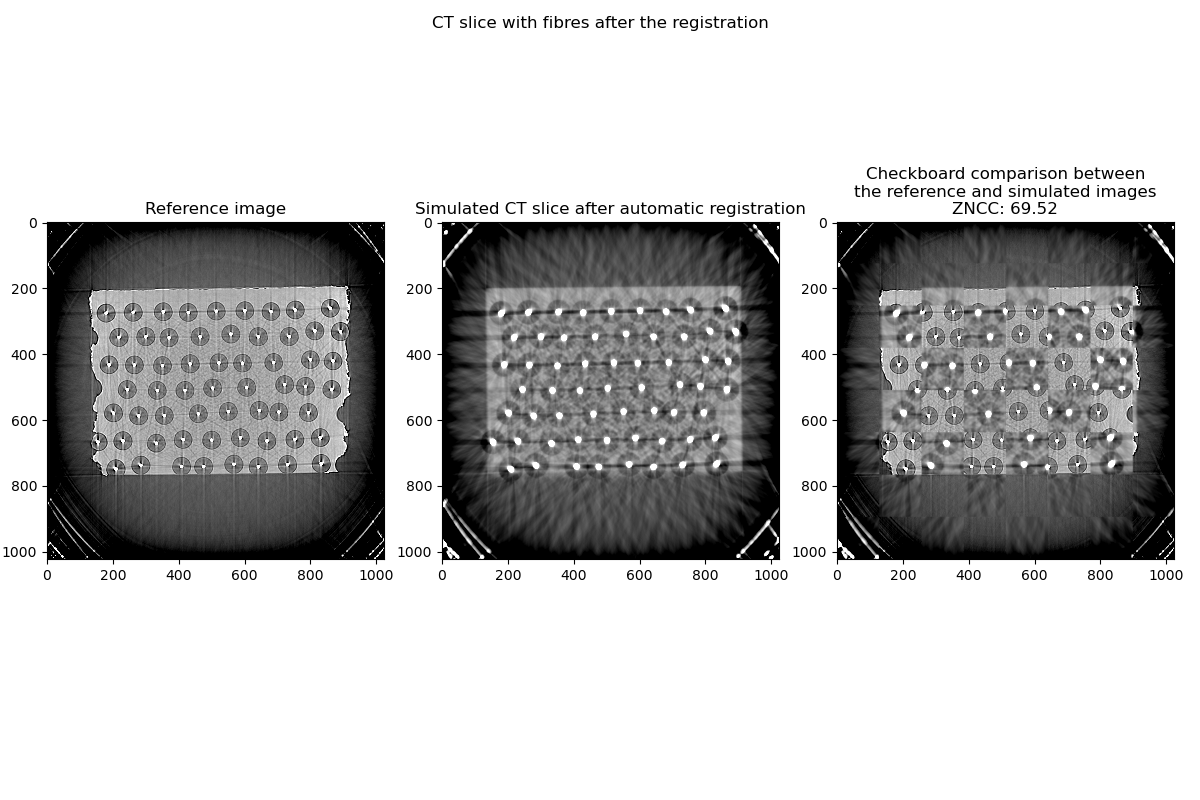
\includegraphics{plots/simulated_CT_slice_with_fibres_after_cube_registration.png}
\caption{Registration of a cube}
\end{figure}

\hypertarget{optimisation-of-the-cores-and-fibres-radii}{%
\section{Optimisation of the cores and fibres
radii}\label{optimisation-of-the-cores-and-fibres-radii}}

    The function below is the objective function used to optimise the radii
of the cores and fibres.

    \begin{tcolorbox}[breakable, size=fbox, boxrule=1pt, pad at break*=1mm,colback=cellbackground, colframe=cellborder]
\prompt{In}{incolor}{58}{\boxspacing}
\begin{Verbatim}[commandchars=\\\{\}]
\PY{k}{def} \PY{n+nf}{fitnessFunctionFibres}\PY{p}{(}\PY{n}{x}\PY{p}{)}\PY{p}{:}
    \PY{k}{global} \PY{n}{best\PYZus{}fitness}\PY{p}{;}
    \PY{k}{global} \PY{n}{best\PYZus{}fitness\PYZus{}id}\PY{p}{;}
    \PY{k}{global} \PY{n}{fibre\PYZus{}radius}\PY{p}{;}
    \PY{k}{global} \PY{n}{core\PYZus{}radius}\PY{p}{;}
    \PY{k}{global} \PY{n}{prefix}\PY{p}{;}

    \PY{c+c1}{\PYZsh{} Get the radii}
    \PY{n}{fibre\PYZus{}radius} \PY{o}{=} \PY{n}{x}\PY{p}{[}\PY{l+m+mi}{0}\PY{p}{]}\PY{p}{;}
    \PY{n}{core\PYZus{}radius} \PY{o}{=} \PY{n}{fibre\PYZus{}radius} \PY{o}{*} \PY{n}{x}\PY{p}{[}\PY{l+m+mi}{1}\PY{p}{]}\PY{p}{;}

    \PY{c+c1}{\PYZsh{} Load the matrix}
    \PY{n}{setMatrix}\PY{p}{(}\PY{n}{matrix\PYZus{}geometry\PYZus{}parameters}\PY{p}{)}\PY{p}{;}

    \PY{c+c1}{\PYZsh{} Load the cores and fibres}
    \PY{n}{setFibres}\PY{p}{(}\PY{n}{centroid\PYZus{}set}\PY{p}{)}\PY{p}{;}

    \PY{c+c1}{\PYZsh{} Simulate a sinogram}
    \PY{n}{simulated\PYZus{}sinogram}\PY{p}{,} \PY{n}{normalised\PYZus{}projections}\PY{p}{,} \PY{n}{raw\PYZus{}projections\PYZus{}in\PYZus{}keV} \PY{o}{=} \PY{n}{simulateSinogram}\PY{p}{(}\PY{n}{sigma\PYZus{}set}\PY{p}{,} \PY{n}{k\PYZus{}set}\PY{p}{,} \PY{n}{label\PYZus{}set}\PY{p}{)}\PY{p}{;}

    \PY{c+c1}{\PYZsh{} Compute the objective value}
    \PY{k}{if} \PY{n}{use\PYZus{}sinogram}\PY{p}{:}
        \PY{n}{objective} \PY{o}{=} \PY{n}{metrics}\PY{p}{(}\PY{n}{reference\PYZus{}sinogram}\PY{p}{,} \PY{n}{simulated\PYZus{}sinogram}\PY{p}{)}\PY{p}{;}
    \PY{k}{else}\PY{p}{:}
        \PY{n}{objective} \PY{o}{=} \PY{n}{metrics}\PY{p}{(}\PY{n}{reference\PYZus{}normalised\PYZus{}projections}\PY{p}{,} \PY{n}{normalised\PYZus{}projections}\PY{p}{)}\PY{p}{;}

    \PY{c+c1}{\PYZsh{} The block below is not necessary for the registration.}
    \PY{c+c1}{\PYZsh{} It is used to save the data to create animations.}
    \PY{k}{if} \PY{n}{best\PYZus{}fitness} \PY{o}{\PYZgt{}} \PY{n}{objective}\PY{p}{:}
        \PY{n}{best\PYZus{}fitness} \PY{o}{=} \PY{n}{objective}\PY{p}{;}
        
        \PY{n}{gvxr}\PY{o}{.}\PY{n}{saveSTLfile}\PY{p}{(}\PY{l+s+s2}{\PYZdq{}}\PY{l+s+s2}{core}\PY{l+s+s2}{\PYZdq{}}\PY{p}{,}  \PY{l+s+s2}{\PYZdq{}}\PY{l+s+s2}{outputs/}\PY{l+s+s2}{\PYZdq{}} \PY{o}{+} \PY{n}{prefix} \PY{o}{+} \PY{n+nb}{str}\PY{p}{(}\PY{n}{best\PYZus{}fitness\PYZus{}id}\PY{p}{)} \PY{o}{+} \PY{l+s+s2}{\PYZdq{}}\PY{l+s+s2}{\PYZus{}cores.stl}\PY{l+s+s2}{\PYZdq{}}\PY{p}{)}\PY{p}{;}
        \PY{n}{gvxr}\PY{o}{.}\PY{n}{saveSTLfile}\PY{p}{(}\PY{l+s+s2}{\PYZdq{}}\PY{l+s+s2}{fibre}\PY{l+s+s2}{\PYZdq{}}\PY{p}{,} \PY{l+s+s2}{\PYZdq{}}\PY{l+s+s2}{outputs/}\PY{l+s+s2}{\PYZdq{}} \PY{o}{+} \PY{n}{prefix} \PY{o}{+} \PY{n+nb}{str}\PY{p}{(}\PY{n}{best\PYZus{}fitness\PYZus{}id}\PY{p}{)} \PY{o}{+} \PY{l+s+s2}{\PYZdq{}}\PY{l+s+s2}{\PYZus{}fibres.stl}\PY{l+s+s2}{\PYZdq{}}\PY{p}{)}\PY{p}{;}
        
        \PY{c+c1}{\PYZsh{} Reconstruct the CT slice}
        \PY{n}{simulated\PYZus{}CT} \PY{o}{=} \PY{n}{tomopy}\PY{o}{.}\PY{n}{recon}\PY{p}{(}\PY{n}{simulated\PYZus{}sinogram}\PY{p}{,}
                                    \PY{n}{theta\PYZus{}rad}\PY{p}{,}
                                    \PY{n}{center}\PY{o}{=}\PY{n}{rot\PYZus{}center}\PY{p}{,}
                                    \PY{n}{sinogram\PYZus{}order}\PY{o}{=}\PY{k+kc}{False}\PY{p}{,}
                                    \PY{n}{algorithm}\PY{o}{=}\PY{l+s+s1}{\PYZsq{}}\PY{l+s+s1}{gridrec}\PY{l+s+s1}{\PYZsq{}}\PY{p}{,}
                                    \PY{n}{filter\PYZus{}name}\PY{o}{=}\PY{l+s+s1}{\PYZsq{}}\PY{l+s+s1}{shepp}\PY{l+s+s1}{\PYZsq{}}\PY{p}{,}
                                    \PY{n}{ncore}\PY{o}{=}\PY{l+m+mi}{40}\PY{p}{)}\PY{p}{[}\PY{l+m+mi}{0}\PY{p}{]}\PY{p}{;}
        
        \PY{c+c1}{\PYZsh{} Save the simulated sinogram}
        \PY{n}{simulated\PYZus{}sinogram}\PY{o}{.}\PY{n}{shape} \PY{o}{=} \PY{p}{(}\PY{n}{simulated\PYZus{}sinogram}\PY{o}{.}\PY{n}{size} \PY{o}{/}\PY{o}{/} \PY{n}{simulated\PYZus{}sinogram}\PY{o}{.}\PY{n}{shape}\PY{p}{[}\PY{l+m+mi}{2}\PY{p}{]}\PY{p}{,} \PY{n}{simulated\PYZus{}sinogram}\PY{o}{.}\PY{n}{shape}\PY{p}{[}\PY{l+m+mi}{2}\PY{p}{]}\PY{p}{)}\PY{p}{;}
        \PY{n}{saveMHA}\PY{p}{(}\PY{l+s+s2}{\PYZdq{}}\PY{l+s+s2}{outputs/}\PY{l+s+s2}{\PYZdq{}} \PY{o}{+} \PY{n}{prefix} \PY{o}{+} \PY{l+s+s2}{\PYZdq{}}\PY{l+s+s2}{simulated\PYZus{}sinogram\PYZus{}}\PY{l+s+s2}{\PYZdq{}} \PY{o}{+} \PY{n+nb}{str}\PY{p}{(}\PY{n}{best\PYZus{}fitness\PYZus{}id}\PY{p}{)} \PY{o}{+} \PY{l+s+s2}{\PYZdq{}}\PY{l+s+s2}{.mha}\PY{l+s+s2}{\PYZdq{}}\PY{p}{,}
                \PY{n}{simulated\PYZus{}sinogram}\PY{p}{,}
                \PY{p}{[}\PY{n}{pixel\PYZus{}spacing\PYZus{}in\PYZus{}mm}\PY{p}{,} \PY{n}{angular\PYZus{}step}\PY{p}{,} \PY{n}{pixel\PYZus{}spacing\PYZus{}in\PYZus{}mm}\PY{p}{]}\PY{p}{)}\PY{p}{;}

        \PY{c+c1}{\PYZsh{} Save the simulated CT slice}
        \PY{n}{saveMHA}\PY{p}{(}\PY{l+s+s2}{\PYZdq{}}\PY{l+s+s2}{outputs/}\PY{l+s+s2}{\PYZdq{}} \PY{o}{+} \PY{n}{prefix} \PY{o}{+} \PY{l+s+s2}{\PYZdq{}}\PY{l+s+s2}{simulated\PYZus{}CT\PYZus{}}\PY{l+s+s2}{\PYZdq{}} \PY{o}{+} \PY{n+nb}{str}\PY{p}{(}\PY{n}{best\PYZus{}fitness\PYZus{}id}\PY{p}{)} \PY{o}{+} \PY{l+s+s2}{\PYZdq{}}\PY{l+s+s2}{.mha}\PY{l+s+s2}{\PYZdq{}}\PY{p}{,}
                \PY{n}{simulated\PYZus{}CT}\PY{p}{,}
                \PY{p}{[}\PY{n}{pixel\PYZus{}spacing\PYZus{}in\PYZus{}mm}\PY{p}{,} \PY{n}{pixel\PYZus{}spacing\PYZus{}in\PYZus{}mm}\PY{p}{,} \PY{n}{pixel\PYZus{}spacing\PYZus{}in\PYZus{}mm}\PY{p}{]}\PY{p}{)}\PY{p}{;}

        \PY{n}{np}\PY{o}{.}\PY{n}{savetxt}\PY{p}{(}\PY{l+s+s2}{\PYZdq{}}\PY{l+s+s2}{outputs/}\PY{l+s+s2}{\PYZdq{}} \PY{o}{+} \PY{n}{prefix} \PY{o}{+} \PY{n+nb}{str}\PY{p}{(}\PY{n}{best\PYZus{}fitness\PYZus{}id}\PY{p}{)} \PY{o}{+} \PY{l+s+s2}{\PYZdq{}}\PY{l+s+s2}{.dat}\PY{l+s+s2}{\PYZdq{}}\PY{p}{,} \PY{n}{x}\PY{p}{,} \PY{n}{header}\PY{o}{=}\PY{l+s+s1}{\PYZsq{}}\PY{l+s+s1}{x,y,rotation\PYZus{}angle,w,h}\PY{l+s+s1}{\PYZsq{}}\PY{p}{)}\PY{p}{;}

        \PY{n}{best\PYZus{}fitness\PYZus{}id} \PY{o}{+}\PY{o}{=} \PY{l+m+mi}{1}\PY{p}{;}

    \PY{k}{return} \PY{n}{objective}
\end{Verbatim}
\end{tcolorbox}

    \begin{tcolorbox}[breakable, size=fbox, boxrule=1pt, pad at break*=1mm,colback=cellbackground, colframe=cellborder]
\prompt{In}{incolor}{59}{\boxspacing}
\begin{Verbatim}[commandchars=\\\{\}]
\PY{c+c1}{\PYZsh{} The registration has already been performed. Load the results.}
\PY{k}{if} \PY{n}{os}\PY{o}{.}\PY{n}{path}\PY{o}{.}\PY{n}{isfile}\PY{p}{(}\PY{l+s+s2}{\PYZdq{}}\PY{l+s+s2}{outputs/fibre1\PYZus{}radii.dat}\PY{l+s+s2}{\PYZdq{}}\PY{p}{)}\PY{p}{:}
    \PY{n}{temp} \PY{o}{=} \PY{n}{np}\PY{o}{.}\PY{n}{loadtxt}\PY{p}{(}\PY{l+s+s2}{\PYZdq{}}\PY{l+s+s2}{outputs/fibre1\PYZus{}radii.dat}\PY{l+s+s2}{\PYZdq{}}\PY{p}{)}\PY{p}{;}
    \PY{n}{core\PYZus{}radius} \PY{o}{=} \PY{n}{temp}\PY{p}{[}\PY{l+m+mi}{0}\PY{p}{]}\PY{p}{;}
    \PY{n}{fibre\PYZus{}radius} \PY{o}{=} \PY{n}{temp}\PY{p}{[}\PY{l+m+mi}{1}\PY{p}{]}\PY{p}{;}
\PY{c+c1}{\PYZsh{} Perform the registration using CMA\PYZhy{}ES}
\PY{k}{else}\PY{p}{:}
    \PY{n}{ratio} \PY{o}{=} \PY{n}{core\PYZus{}radius} \PY{o}{/} \PY{n}{fibre\PYZus{}radius}\PY{p}{;}

    \PY{n}{x0} \PY{o}{=} \PY{p}{[}\PY{n}{fibre\PYZus{}radius}\PY{p}{,} \PY{n}{ratio}\PY{p}{]}\PY{p}{;}
    \PY{n}{bounds} \PY{o}{=} \PY{p}{[}\PY{p}{[}\PY{l+m+mi}{5}\PY{p}{,} \PY{l+m+mf}{0.01}\PY{p}{]}\PY{p}{,} \PY{p}{[}\PY{l+m+mf}{1.5} \PY{o}{*} \PY{n}{fibre\PYZus{}radius}\PY{p}{,} \PY{l+m+mf}{0.95}\PY{p}{]}\PY{p}{]}\PY{p}{;}

    \PY{n}{best\PYZus{}fitness} \PY{o}{=} \PY{n}{sys}\PY{o}{.}\PY{n}{float\PYZus{}info}\PY{o}{.}\PY{n}{max}\PY{p}{;}
    \PY{n}{best\PYZus{}fitness\PYZus{}id} \PY{o}{=} \PY{l+m+mi}{0}\PY{p}{;}
    \PY{n}{prefix} \PY{o}{=} \PY{l+s+s2}{\PYZdq{}}\PY{l+s+s2}{fibre1\PYZus{}}\PY{l+s+s2}{\PYZdq{}}\PY{p}{;}
    
    \PY{n}{opts} \PY{o}{=} \PY{n}{cma}\PY{o}{.}\PY{n}{CMAOptions}\PY{p}{(}\PY{p}{)}
    \PY{n}{opts}\PY{o}{.}\PY{n}{set}\PY{p}{(}\PY{l+s+s1}{\PYZsq{}}\PY{l+s+s1}{tolfun}\PY{l+s+s1}{\PYZsq{}}\PY{p}{,} \PY{l+m+mf}{1e\PYZhy{}3}\PY{p}{)}\PY{p}{;}
    \PY{n}{opts}\PY{p}{[}\PY{l+s+s1}{\PYZsq{}}\PY{l+s+s1}{tolx}\PY{l+s+s1}{\PYZsq{}}\PY{p}{]} \PY{o}{=} \PY{l+m+mf}{1e\PYZhy{}3}\PY{p}{;}
    \PY{n}{opts}\PY{p}{[}\PY{l+s+s1}{\PYZsq{}}\PY{l+s+s1}{bounds}\PY{l+s+s1}{\PYZsq{}}\PY{p}{]} \PY{o}{=} \PY{n}{bounds}\PY{p}{;}

    \PY{n}{es} \PY{o}{=} \PY{n}{cma}\PY{o}{.}\PY{n}{CMAEvolutionStrategy}\PY{p}{(}\PY{n}{x0}\PY{p}{,} \PY{l+m+mf}{0.9}\PY{p}{,} \PY{n}{opts}\PY{p}{)}\PY{p}{;}
    \PY{n}{es}\PY{o}{.}\PY{n}{optimize}\PY{p}{(}\PY{n}{fitnessFunctionFibres}\PY{p}{)}\PY{p}{;}
    \PY{n}{fibre\PYZus{}radius} \PY{o}{=} \PY{n}{es}\PY{o}{.}\PY{n}{result}\PY{o}{.}\PY{n}{xbest}\PY{p}{[}\PY{l+m+mi}{0}\PY{p}{]}\PY{p}{;}
    \PY{n}{core\PYZus{}radius} \PY{o}{=} \PY{n}{fibre\PYZus{}radius} \PY{o}{*} \PY{n}{es}\PY{o}{.}\PY{n}{result}\PY{o}{.}\PY{n}{xbest}\PY{p}{[}\PY{l+m+mi}{1}\PY{p}{]}\PY{p}{;}

    \PY{n}{np}\PY{o}{.}\PY{n}{savetxt}\PY{p}{(}\PY{l+s+s2}{\PYZdq{}}\PY{l+s+s2}{outputs/fibre1\PYZus{}radii.dat}\PY{l+s+s2}{\PYZdq{}}\PY{p}{,} \PY{p}{[}\PY{n}{core\PYZus{}radius}\PY{p}{,} \PY{n}{fibre\PYZus{}radius}\PY{p}{]}\PY{p}{,} \PY{n}{header}\PY{o}{=}\PY{l+s+s1}{\PYZsq{}}\PY{l+s+s1}{core\PYZus{}radius\PYZus{}in\PYZus{}um,fibre\PYZus{}radius\PYZus{}in\PYZus{}um}\PY{l+s+s1}{\PYZsq{}}\PY{p}{)}\PY{p}{;}
    
    \PY{c+c1}{\PYZsh{} Release memory}
    \PY{k}{del} \PY{n}{es}\PY{p}{;}
\end{Verbatim}
\end{tcolorbox}

    \begin{Verbatim}[commandchars=\\\{\}]
(3\_w,6)-aCMA-ES (mu\_w=2.0,w\_1=63\%) in dimension 2 (seed=203307, Tue Jun  8
20:30:26 2021)
Iterat \#Fevals   function value  axis ratio  sigma  min\&max std  t[m:s]
    1      6 2.895655461031801e-01 1.0e+00 7.66e-01  7e-01  7e-01 0:08.3
    2     12 2.350046077132609e-01 1.2e+00 6.52e-01  5e-01  5e-01 0:16.3
    3     18 2.038963702735447e-01 1.2e+00 5.60e-01  4e-01  5e-01 0:23.9
    4     24 3.365074065580562e-01 1.2e+00 5.07e-01  4e-01  4e-01 0:31.1
    5     30 3.528799764412728e-01 1.2e+00 6.22e-01  4e-01  6e-01 0:38.3
    6     36 2.796072738821871e-01 1.4e+00 5.44e-01  4e-01  5e-01 0:45.7
    7     42 2.307486626427863e-01 1.3e+00 5.36e-01  4e-01  4e-01 0:53.0
    8     48 2.109749623076709e-01 1.1e+00 4.13e-01  3e-01  3e-01 1:00.2
   10     60 2.155547815741161e-01 1.1e+00 3.86e-01  2e-01  3e-01 1:14.7
   12     72 2.621247334067883e-01 1.3e+00 2.40e-01  1e-01  1e-01 1:29.2
   14     84 2.124465644617283e-01 1.4e+00 1.74e-01  6e-02  9e-02 1:43.9
   16     96 2.124210383423197e-01 2.4e+00 2.00e-01  5e-02  1e-01 1:58.4
   18    108 2.108204351034491e-01 3.9e+00 1.57e-01  2e-02  1e-01 2:12.9
   20    120 2.100611230400567e-01 7.1e+00 1.71e-01  2e-02  1e-01 2:29.9
   22    132 2.068443000861420e-01 1.2e+01 2.29e-01  2e-02  3e-01 2:44.6
   25    150 1.927938147247228e-01 3.5e+01 5.58e-01  3e-02  1e+00 3:05.8
   28    168 1.749698968154965e-01 5.6e+01 9.33e-01  3e-02  2e+00 3:26.9
   31    186 1.542019850326830e-01 9.8e+01 9.79e-01  2e-02  2e+00 3:48.1
   34    204 1.302989051475420e-01 1.9e+02 1.46e+00  2e-02  4e+00 4:09.2
   37    222 1.251928909130225e-01 2.7e+02 2.14e+00  2e-02  6e+00 4:30.1
   40    240 1.228684759140323e-01 2.7e+02 1.80e+00  2e-02  4e+00 4:50.2
   44    264 1.215144816868614e-01 4.9e+02 1.03e+00  7e-03  2e+00 5:17.6
   48    288 1.214250157595831e-01 4.3e+02 4.90e-01  3e-03  7e-01 5:45.4
   52    312 1.213838336023714e-01 6.3e+02 2.22e-01  8e-04  2e-01 6:13.6
   56    336 1.213837669983424e-01 5.9e+02 1.37e-01  5e-04  9e-02 6:41.1
   60    360 1.213782394557764e-01 6.9e+02 1.71e-01  6e-04  1e-01 7:08.5
    \end{Verbatim}

    \begin{tcolorbox}[breakable, size=fbox, boxrule=1pt, pad at break*=1mm,colback=cellbackground, colframe=cellborder]
\prompt{In}{incolor}{60}{\boxspacing}
\begin{Verbatim}[commandchars=\\\{\}]
\PY{k}{if} \PY{o+ow}{not} \PY{n}{os}\PY{o}{.}\PY{n}{path}\PY{o}{.}\PY{n}{exists}\PY{p}{(}\PY{l+s+s2}{\PYZdq{}}\PY{l+s+s2}{plots/fibre1\PYZus{}registration.gif}\PY{l+s+s2}{\PYZdq{}}\PY{p}{)}\PY{p}{:}
    \PY{n}{registration\PYZus{}image\PYZus{}set} \PY{o}{=} \PY{n}{createAnimation}\PY{p}{(}\PY{l+s+s2}{\PYZdq{}}\PY{l+s+s2}{outputs/fibre1\PYZus{}simulated\PYZus{}CT\PYZus{}}\PY{l+s+s2}{\PYZdq{}}\PY{p}{,}
                \PY{l+s+s1}{\PYZsq{}}\PY{l+s+s1}{plots/fibre1\PYZus{}registration.gif}\PY{l+s+s1}{\PYZsq{}}\PY{p}{)}\PY{p}{;}
\end{Verbatim}
\end{tcolorbox}

    \begin{figure}
\centering
\includegraphics{plots/fibre1_registration-39}
\caption{Animation of the registration (GIF file)}
\end{figure}

    \hypertarget{apply-the-result-of-the-registration}{%
\subsection{Apply the result of the
registration}\label{apply-the-result-of-the-registration}}

    \begin{tcolorbox}[breakable, size=fbox, boxrule=1pt, pad at break*=1mm,colback=cellbackground, colframe=cellborder]
\prompt{In}{incolor}{61}{\boxspacing}
\begin{Verbatim}[commandchars=\\\{\}]
\PY{c+c1}{\PYZsh{} Load the matrix}
\PY{n}{setMatrix}\PY{p}{(}\PY{n}{matrix\PYZus{}geometry\PYZus{}parameters}\PY{p}{)}\PY{p}{;}

\PY{c+c1}{\PYZsh{} Load the cores and fibres}
\PY{n}{setFibres}\PY{p}{(}\PY{n}{centroid\PYZus{}set}\PY{p}{)}\PY{p}{;}

\PY{n}{gvxr}\PY{o}{.}\PY{n}{saveSTLfile}\PY{p}{(}\PY{l+s+s2}{\PYZdq{}}\PY{l+s+s2}{fibre}\PY{l+s+s2}{\PYZdq{}}\PY{p}{,} \PY{l+s+s2}{\PYZdq{}}\PY{l+s+s2}{outputs/fibre1\PYZus{}fibre.stl}\PY{l+s+s2}{\PYZdq{}}\PY{p}{)}\PY{p}{;}
\PY{n}{gvxr}\PY{o}{.}\PY{n}{saveSTLfile}\PY{p}{(}\PY{l+s+s2}{\PYZdq{}}\PY{l+s+s2}{core}\PY{l+s+s2}{\PYZdq{}}\PY{p}{,}  \PY{l+s+s2}{\PYZdq{}}\PY{l+s+s2}{outputs/fibre1\PYZus{}core.stl}\PY{l+s+s2}{\PYZdq{}}\PY{p}{)}\PY{p}{;}

\PY{n+nb}{print}\PY{p}{(}\PY{l+s+s2}{\PYZdq{}}\PY{l+s+s2}{Core diameter:}\PY{l+s+s2}{\PYZdq{}}\PY{p}{,} \PY{n+nb}{round}\PY{p}{(}\PY{n}{core\PYZus{}radius} \PY{o}{*} \PY{l+m+mi}{2}\PY{p}{)}\PY{p}{,} \PY{l+s+s2}{\PYZdq{}}\PY{l+s+s2}{um}\PY{l+s+s2}{\PYZdq{}}\PY{p}{)}\PY{p}{;}
\PY{n+nb}{print}\PY{p}{(}\PY{l+s+s2}{\PYZdq{}}\PY{l+s+s2}{Fibre diameter:}\PY{l+s+s2}{\PYZdq{}}\PY{p}{,} \PY{n+nb}{round}\PY{p}{(}\PY{n}{fibre\PYZus{}radius} \PY{o}{*} \PY{l+m+mi}{2}\PY{p}{)}\PY{p}{,} \PY{l+s+s2}{\PYZdq{}}\PY{l+s+s2}{um}\PY{l+s+s2}{\PYZdq{}}\PY{p}{)}\PY{p}{;}

\PY{c+c1}{\PYZsh{} Simulate the corresponding CT aquisition}
\PY{n}{simulated\PYZus{}sinogram}\PY{p}{,} \PY{n}{normalised\PYZus{}projections}\PY{p}{,} \PY{n}{raw\PYZus{}projections\PYZus{}in\PYZus{}keV} \PY{o}{=} \PY{n}{simulateSinogram}\PY{p}{(}\PY{n}{sigma\PYZus{}set}\PY{p}{,} \PY{n}{k\PYZus{}set}\PY{p}{,} \PY{n}{label\PYZus{}set}\PY{p}{)}\PY{p}{;}

\PY{c+c1}{\PYZsh{} Reconstruct the CT slice}
\PY{n}{simulated\PYZus{}CT} \PY{o}{=} \PY{n}{tomopy}\PY{o}{.}\PY{n}{recon}\PY{p}{(}\PY{n}{simulated\PYZus{}sinogram}\PY{p}{,}
                            \PY{n}{theta\PYZus{}rad}\PY{p}{,}
                            \PY{n}{center}\PY{o}{=}\PY{n}{rot\PYZus{}center}\PY{p}{,}
                            \PY{n}{sinogram\PYZus{}order}\PY{o}{=}\PY{k+kc}{False}\PY{p}{,}
                            \PY{n}{algorithm}\PY{o}{=}\PY{l+s+s1}{\PYZsq{}}\PY{l+s+s1}{gridrec}\PY{l+s+s1}{\PYZsq{}}\PY{p}{,}
                            \PY{n}{filter\PYZus{}name}\PY{o}{=}\PY{l+s+s1}{\PYZsq{}}\PY{l+s+s1}{shepp}\PY{l+s+s1}{\PYZsq{}}\PY{p}{,}
                            \PY{n}{ncore}\PY{o}{=}\PY{l+m+mi}{40}\PY{p}{)}\PY{p}{[}\PY{l+m+mi}{0}\PY{p}{]}\PY{p}{;}
\PY{n}{normalised\PYZus{}simulated\PYZus{}CT} \PY{o}{=} \PY{n}{standardisation}\PY{p}{(}\PY{n}{simulated\PYZus{}CT}\PY{p}{)}\PY{p}{;}


\PY{c+c1}{\PYZsh{} Compute the ZNCC}
\PY{n+nb}{print}\PY{p}{(}\PY{l+s+s2}{\PYZdq{}}\PY{l+s+s2}{ZNCC radii registration 1:}\PY{l+s+s2}{\PYZdq{}}\PY{p}{,}
      \PY{l+s+s2}{\PYZdq{}}\PY{l+s+si}{\PYZob{}:.2f\PYZcb{}}\PY{l+s+s2}{\PYZdq{}}\PY{o}{.}\PY{n}{format}\PY{p}{(}\PY{l+m+mf}{100.0} \PY{o}{*} \PY{n}{np}\PY{o}{.}\PY{n}{mean}\PY{p}{(}\PY{n}{np}\PY{o}{.}\PY{n}{multiply}\PY{p}{(}\PY{n}{normalised\PYZus{}reference\PYZus{}CT}\PY{p}{,} \PY{n}{normalised\PYZus{}simulated\PYZus{}CT}\PY{p}{)}\PY{p}{)}\PY{p}{)}\PY{p}{)}\PY{p}{;}
\end{Verbatim}
\end{tcolorbox}

    \begin{Verbatim}[commandchars=\\\{\}]
Core diameter: 16 um
Fibre diameter: 102 um
ZNCC radii registration 1: 90.28
    \end{Verbatim}

    The 3D view of the registration looks like:

\begin{figure}
\centering
\includegraphics{./3d-view.png}
\caption{3D view}
\end{figure}

    \hypertarget{recentre-each-corefibre}{%
\section{Recentre each core/fibre}\label{recentre-each-corefibre}}

    Each fibre is extracted from both the reference CT slice and simulated
CT slice. The displacement between the corresponding fibres is computed
to maximise the ZNCC between the two. The centre of the fibre is then
adjusted accordingly.

    \begin{tcolorbox}[breakable, size=fbox, boxrule=1pt, pad at break*=1mm,colback=cellbackground, colframe=cellborder]
\prompt{In}{incolor}{62}{\boxspacing}
\begin{Verbatim}[commandchars=\\\{\}]
\PY{k}{def} \PY{n+nf}{refineCentrePositions}\PY{p}{(}\PY{n}{centroid\PYZus{}set}\PY{p}{,} \PY{n}{reconstruction\PYZus{}CT\PYZus{}fibres}\PY{p}{)}\PY{p}{:}

    \PY{c+c1}{\PYZsh{} Exhaustive local search to refine the centre of each cylinder}
    \PY{n}{roi\PYZus{}length} \PY{o}{=} \PY{l+m+mi}{40}\PY{p}{;}
    \PY{n}{new\PYZus{}centroid\PYZus{}set} \PY{o}{=} \PY{p}{[}\PY{p}{]}\PY{p}{;}
    \PY{k}{for} \PY{n}{i}\PY{p}{,} \PY{n}{cyl} \PY{o+ow}{in} \PY{n+nb}{enumerate}\PY{p}{(}\PY{n}{centroid\PYZus{}set}\PY{p}{)}\PY{p}{:}

        \PY{n}{centre} \PY{o}{=} \PY{p}{[}
            \PY{n}{cyl}\PY{p}{[}\PY{l+m+mi}{0}\PY{p}{]}\PY{p}{,}
            \PY{n}{cyl}\PY{p}{[}\PY{l+m+mi}{1}\PY{p}{]}
        \PY{p}{]}\PY{p}{;}

        \PY{c+c1}{\PYZsh{} extract ROI from reference image}
        \PY{n}{reference\PYZus{}image} \PY{o}{=} \PY{n}{copy}\PY{o}{.}\PY{n}{deepcopy}\PY{p}{(}\PY{n}{reference\PYZus{}CT}\PY{p}{[}\PY{n}{centre}\PY{p}{[}\PY{l+m+mi}{1}\PY{p}{]} \PY{o}{\PYZhy{}} \PY{n}{roi\PYZus{}length}\PY{p}{:}\PY{n}{centre}\PY{p}{[}\PY{l+m+mi}{1}\PY{p}{]} \PY{o}{+} \PY{n}{roi\PYZus{}length}\PY{p}{,} \PY{n}{centre}\PY{p}{[}\PY{l+m+mi}{0}\PY{p}{]} \PY{o}{\PYZhy{}} \PY{n}{roi\PYZus{}length}\PY{p}{:}\PY{n}{centre}\PY{p}{[}\PY{l+m+mi}{0}\PY{p}{]} \PY{o}{+} \PY{n}{roi\PYZus{}length}\PY{p}{]}\PY{p}{)}\PY{p}{;}

        \PY{c+c1}{\PYZsh{} Normalise ROI}
        \PY{n}{reference\PYZus{}image} \PY{o}{=} \PY{n}{standardisation}\PY{p}{(}\PY{n}{reference\PYZus{}image}\PY{p}{)}\PY{p}{;}

        \PY{n}{best\PYZus{}ZNCC} \PY{o}{=} \PY{o}{\PYZhy{}}\PY{l+m+mi}{1}\PY{p}{;}
        \PY{n}{best\PYZus{}x\PYZus{}offset} \PY{o}{=} \PY{l+m+mi}{0}\PY{p}{;}
        \PY{n}{best\PYZus{}y\PYZus{}offset} \PY{o}{=} \PY{l+m+mi}{0}\PY{p}{;}

        \PY{k}{for} \PY{n}{y} \PY{o+ow}{in} \PY{n+nb}{range}\PY{p}{(}\PY{o}{\PYZhy{}}\PY{l+m+mi}{10}\PY{p}{,} \PY{l+m+mi}{11}\PY{p}{)}\PY{p}{:}
            \PY{k}{for} \PY{n}{x} \PY{o+ow}{in} \PY{n+nb}{range}\PY{p}{(}\PY{o}{\PYZhy{}}\PY{l+m+mi}{10}\PY{p}{,} \PY{l+m+mi}{11}\PY{p}{)}\PY{p}{:}

                \PY{n}{centre} \PY{o}{=} \PY{p}{[}
                    \PY{n}{cyl}\PY{p}{[}\PY{l+m+mi}{0}\PY{p}{]} \PY{o}{+} \PY{n}{x}\PY{p}{,}
                    \PY{n}{cyl}\PY{p}{[}\PY{l+m+mi}{1}\PY{p}{]} \PY{o}{+} \PY{n}{y}
                \PY{p}{]}\PY{p}{;}

                \PY{c+c1}{\PYZsh{} extract ROI from test image}
                \PY{n}{test\PYZus{}image} \PY{o}{=} \PY{n}{copy}\PY{o}{.}\PY{n}{deepcopy}\PY{p}{(}\PY{n}{reconstruction\PYZus{}CT\PYZus{}fibres}\PY{p}{[}\PY{n}{centre}\PY{p}{[}\PY{l+m+mi}{1}\PY{p}{]} \PY{o}{\PYZhy{}} \PY{n}{roi\PYZus{}length}\PY{p}{:}\PY{n}{centre}\PY{p}{[}\PY{l+m+mi}{1}\PY{p}{]} \PY{o}{+} \PY{n}{roi\PYZus{}length}\PY{p}{,} \PY{n}{centre}\PY{p}{[}\PY{l+m+mi}{0}\PY{p}{]} \PY{o}{\PYZhy{}} \PY{n}{roi\PYZus{}length}\PY{p}{:}\PY{n}{centre}\PY{p}{[}\PY{l+m+mi}{0}\PY{p}{]} \PY{o}{+} \PY{n}{roi\PYZus{}length}\PY{p}{]}\PY{p}{)}\PY{p}{;}

                \PY{c+c1}{\PYZsh{} Normalise ROI}
                \PY{n}{test\PYZus{}image} \PY{o}{=} \PY{n}{standardisation}\PY{p}{(}\PY{n}{test\PYZus{}image}\PY{p}{)}\PY{p}{;}

                \PY{c+c1}{\PYZsh{} Compare the ROIs}
                \PY{n}{zncc} \PY{o}{=} \PY{n}{np}\PY{o}{.}\PY{n}{mean}\PY{p}{(}\PY{n}{np}\PY{o}{.}\PY{n}{multiply}\PY{p}{(}\PY{n}{reference\PYZus{}image}\PY{o}{.}\PY{n}{flatten}\PY{p}{(}\PY{p}{)}\PY{p}{,} \PY{n}{test\PYZus{}image}\PY{o}{.}\PY{n}{flatten}\PY{p}{(}\PY{p}{)}\PY{p}{)}\PY{p}{)}\PY{p}{;}

                \PY{k}{if} \PY{n}{best\PYZus{}ZNCC} \PY{o}{\PYZlt{}} \PY{n}{zncc}\PY{p}{:}
                    \PY{n}{best\PYZus{}ZNCC} \PY{o}{=} \PY{n}{zncc}\PY{p}{;}
                    \PY{n}{best\PYZus{}x\PYZus{}offset} \PY{o}{=} \PY{n}{x}\PY{p}{;}
                    \PY{n}{best\PYZus{}y\PYZus{}offset} \PY{o}{=} \PY{n}{y}\PY{p}{;}

        \PY{c+c1}{\PYZsh{} Correct the position of the centre of the fibre}
        \PY{n}{new\PYZus{}centroid\PYZus{}set}\PY{o}{.}\PY{n}{append}\PY{p}{(}\PY{p}{[}\PY{n}{cyl}\PY{p}{[}\PY{l+m+mi}{0}\PY{p}{]} \PY{o}{\PYZhy{}} \PY{n}{best\PYZus{}x\PYZus{}offset}\PY{p}{,} \PY{n}{cyl}\PY{p}{[}\PY{l+m+mi}{1}\PY{p}{]} \PY{o}{\PYZhy{}} \PY{n}{best\PYZus{}y\PYZus{}offset}\PY{p}{]}\PY{p}{)}\PY{p}{;}

    \PY{k}{return} \PY{n}{new\PYZus{}centroid\PYZus{}set}\PY{p}{;}
\end{Verbatim}
\end{tcolorbox}

    \begin{tcolorbox}[breakable, size=fbox, boxrule=1pt, pad at break*=1mm,colback=cellbackground, colframe=cellborder]
\prompt{In}{incolor}{63}{\boxspacing}
\begin{Verbatim}[commandchars=\\\{\}]
\PY{n}{centroid\PYZus{}set} \PY{o}{=} \PY{n}{refineCentrePositions}\PY{p}{(}\PY{n}{centroid\PYZus{}set}\PY{p}{,} \PY{n}{normalised\PYZus{}simulated\PYZus{}CT}\PY{p}{)}\PY{p}{;}
\end{Verbatim}
\end{tcolorbox}

    \hypertarget{applying-the-result-of-recentring}{%
\subsection{Applying the result of
recentring}\label{applying-the-result-of-recentring}}

    \begin{tcolorbox}[breakable, size=fbox, boxrule=1pt, pad at break*=1mm,colback=cellbackground, colframe=cellborder]
\prompt{In}{incolor}{64}{\boxspacing}
\begin{Verbatim}[commandchars=\\\{\}]
\PY{c+c1}{\PYZsh{} Load the matrix}
\PY{n}{setMatrix}\PY{p}{(}\PY{n}{matrix\PYZus{}geometry\PYZus{}parameters}\PY{p}{)}\PY{p}{;}

\PY{c+c1}{\PYZsh{} Load the cores and fibres}
\PY{n}{setFibres}\PY{p}{(}\PY{n}{centroid\PYZus{}set}\PY{p}{)}\PY{p}{;}

\PY{n}{gvxr}\PY{o}{.}\PY{n}{saveSTLfile}\PY{p}{(}\PY{l+s+s2}{\PYZdq{}}\PY{l+s+s2}{fibre}\PY{l+s+s2}{\PYZdq{}}\PY{p}{,} \PY{l+s+s2}{\PYZdq{}}\PY{l+s+s2}{outputs/fibre2\PYZus{}fibre.stl}\PY{l+s+s2}{\PYZdq{}}\PY{p}{)}\PY{p}{;}
\PY{n}{gvxr}\PY{o}{.}\PY{n}{saveSTLfile}\PY{p}{(}\PY{l+s+s2}{\PYZdq{}}\PY{l+s+s2}{core}\PY{l+s+s2}{\PYZdq{}}\PY{p}{,}  \PY{l+s+s2}{\PYZdq{}}\PY{l+s+s2}{outputs/fibre2\PYZus{}core.stl}\PY{l+s+s2}{\PYZdq{}}\PY{p}{)}\PY{p}{;}

\PY{c+c1}{\PYZsh{} Simulate the corresponding CT aquisition}
\PY{n}{simulated\PYZus{}sinogram}\PY{p}{,} \PY{n}{normalised\PYZus{}projections}\PY{p}{,} \PY{n}{raw\PYZus{}projections\PYZus{}in\PYZus{}keV} \PY{o}{=} \PY{n}{simulateSinogram}\PY{p}{(}\PY{n}{sigma\PYZus{}set}\PY{p}{,} \PY{n}{k\PYZus{}set}\PY{p}{,} \PY{n}{label\PYZus{}set}\PY{p}{)}\PY{p}{;}

\PY{c+c1}{\PYZsh{} Reconstruct the CT slice}
\PY{n}{simulated\PYZus{}CT} \PY{o}{=} \PY{n}{tomopy}\PY{o}{.}\PY{n}{recon}\PY{p}{(}\PY{n}{simulated\PYZus{}sinogram}\PY{p}{,}
                            \PY{n}{theta\PYZus{}rad}\PY{p}{,}
                            \PY{n}{center}\PY{o}{=}\PY{n}{rot\PYZus{}center}\PY{p}{,}
                            \PY{n}{sinogram\PYZus{}order}\PY{o}{=}\PY{k+kc}{False}\PY{p}{,}
                            \PY{n}{algorithm}\PY{o}{=}\PY{l+s+s1}{\PYZsq{}}\PY{l+s+s1}{gridrec}\PY{l+s+s1}{\PYZsq{}}\PY{p}{,}
                            \PY{n}{filter\PYZus{}name}\PY{o}{=}\PY{l+s+s1}{\PYZsq{}}\PY{l+s+s1}{shepp}\PY{l+s+s1}{\PYZsq{}}\PY{p}{,}
                            \PY{n}{ncore}\PY{o}{=}\PY{l+m+mi}{40}\PY{p}{)}\PY{p}{[}\PY{l+m+mi}{0}\PY{p}{]}\PY{p}{;}
\PY{n}{normalised\PYZus{}simulated\PYZus{}CT} \PY{o}{=} \PY{n}{standardisation}\PY{p}{(}\PY{n}{simulated\PYZus{}CT}\PY{p}{)}\PY{p}{;}

\PY{c+c1}{\PYZsh{} Compute the ZNCC}
\PY{n+nb}{print}\PY{p}{(}\PY{l+s+s2}{\PYZdq{}}\PY{l+s+s2}{ZNCC recentring registration:}\PY{l+s+s2}{\PYZdq{}}\PY{p}{,}
      \PY{l+s+s2}{\PYZdq{}}\PY{l+s+si}{\PYZob{}:.2f\PYZcb{}}\PY{l+s+s2}{\PYZdq{}}\PY{o}{.}\PY{n}{format}\PY{p}{(}\PY{l+m+mf}{100.0} \PY{o}{*} \PY{n}{np}\PY{o}{.}\PY{n}{mean}\PY{p}{(}\PY{n}{np}\PY{o}{.}\PY{n}{multiply}\PY{p}{(}\PY{n}{normalised\PYZus{}reference\PYZus{}CT}\PY{p}{,} \PY{n}{normalised\PYZus{}simulated\PYZus{}CT}\PY{p}{)}\PY{p}{)}\PY{p}{)}\PY{p}{)}\PY{p}{;}
\end{Verbatim}
\end{tcolorbox}

    \begin{Verbatim}[commandchars=\\\{\}]
ZNCC recentring registration: 90.94
    \end{Verbatim}

    \hypertarget{optimisation-the-radii-after-recentring}{%
\section{Optimisation the radii after
recentring}\label{optimisation-the-radii-after-recentring}}

    After recentring the centres, another run of optimisation is executed to
refine the radii of the fibres and cores.

    \begin{tcolorbox}[breakable, size=fbox, boxrule=1pt, pad at break*=1mm,colback=cellbackground, colframe=cellborder]
\prompt{In}{incolor}{65}{\boxspacing}
\begin{Verbatim}[commandchars=\\\{\}]
\PY{c+c1}{\PYZsh{} The registration has already been performed. Load the results.}
\PY{k}{if} \PY{n}{os}\PY{o}{.}\PY{n}{path}\PY{o}{.}\PY{n}{isfile}\PY{p}{(}\PY{l+s+s2}{\PYZdq{}}\PY{l+s+s2}{outputs/fibre3\PYZus{}radii.dat}\PY{l+s+s2}{\PYZdq{}}\PY{p}{)}\PY{p}{:}
    \PY{n}{temp} \PY{o}{=} \PY{n}{np}\PY{o}{.}\PY{n}{loadtxt}\PY{p}{(}\PY{l+s+s2}{\PYZdq{}}\PY{l+s+s2}{outputs/fibre3\PYZus{}radii.dat}\PY{l+s+s2}{\PYZdq{}}\PY{p}{)}\PY{p}{;}
    \PY{n}{core\PYZus{}radius} \PY{o}{=} \PY{n}{temp}\PY{p}{[}\PY{l+m+mi}{0}\PY{p}{]}\PY{p}{;}
    \PY{n}{fibre\PYZus{}radius} \PY{o}{=} \PY{n}{temp}\PY{p}{[}\PY{l+m+mi}{1}\PY{p}{]}\PY{p}{;}
\PY{c+c1}{\PYZsh{} Perform the registration using CMA\PYZhy{}ES}
\PY{k}{else}\PY{p}{:}
    \PY{n}{ratio} \PY{o}{=} \PY{n}{core\PYZus{}radius} \PY{o}{/} \PY{n}{fibre\PYZus{}radius}\PY{p}{;}

    \PY{n}{x0} \PY{o}{=} \PY{p}{[}\PY{n}{fibre\PYZus{}radius}\PY{p}{,} \PY{n}{ratio}\PY{p}{]}\PY{p}{;}
    \PY{n}{bounds} \PY{o}{=} \PY{p}{[}\PY{p}{[}\PY{l+m+mi}{5}\PY{p}{,} \PY{l+m+mf}{0.01}\PY{p}{]}\PY{p}{,} \PY{p}{[}\PY{l+m+mf}{1.5} \PY{o}{*} \PY{n}{fibre\PYZus{}radius}\PY{p}{,} \PY{l+m+mf}{0.95}\PY{p}{]}\PY{p}{]}\PY{p}{;}

    \PY{n}{best\PYZus{}fitness} \PY{o}{=} \PY{n}{sys}\PY{o}{.}\PY{n}{float\PYZus{}info}\PY{o}{.}\PY{n}{max}\PY{p}{;}
    \PY{n}{best\PYZus{}fitness\PYZus{}id} \PY{o}{=} \PY{l+m+mi}{0}\PY{p}{;}
    \PY{n}{prefix} \PY{o}{=} \PY{l+s+s2}{\PYZdq{}}\PY{l+s+s2}{fibre3\PYZus{}}\PY{l+s+s2}{\PYZdq{}}\PY{p}{;}

    \PY{n}{opts} \PY{o}{=} \PY{n}{cma}\PY{o}{.}\PY{n}{CMAOptions}\PY{p}{(}\PY{p}{)}
    \PY{n}{opts}\PY{o}{.}\PY{n}{set}\PY{p}{(}\PY{l+s+s1}{\PYZsq{}}\PY{l+s+s1}{tolfun}\PY{l+s+s1}{\PYZsq{}}\PY{p}{,} \PY{l+m+mf}{1e\PYZhy{}2}\PY{p}{)}\PY{p}{;}
    \PY{n}{opts}\PY{p}{[}\PY{l+s+s1}{\PYZsq{}}\PY{l+s+s1}{tolx}\PY{l+s+s1}{\PYZsq{}}\PY{p}{]} \PY{o}{=} \PY{l+m+mf}{1e\PYZhy{}2}\PY{p}{;}
    \PY{n}{opts}\PY{p}{[}\PY{l+s+s1}{\PYZsq{}}\PY{l+s+s1}{bounds}\PY{l+s+s1}{\PYZsq{}}\PY{p}{]} \PY{o}{=} \PY{n}{bounds}\PY{p}{;}

    \PY{n}{es} \PY{o}{=} \PY{n}{cma}\PY{o}{.}\PY{n}{CMAEvolutionStrategy}\PY{p}{(}\PY{n}{x0}\PY{p}{,} \PY{l+m+mf}{0.9}\PY{p}{,} \PY{n}{opts}\PY{p}{)}\PY{p}{;}
    \PY{n}{es}\PY{o}{.}\PY{n}{optimize}\PY{p}{(}\PY{n}{fitnessFunctionFibres}\PY{p}{)}\PY{p}{;}
    \PY{n}{fibre\PYZus{}radius} \PY{o}{=} \PY{n}{es}\PY{o}{.}\PY{n}{result}\PY{o}{.}\PY{n}{xbest}\PY{p}{[}\PY{l+m+mi}{0}\PY{p}{]}\PY{p}{;}
    \PY{n}{core\PYZus{}radius} \PY{o}{=} \PY{n}{fibre\PYZus{}radius} \PY{o}{*} \PY{n}{es}\PY{o}{.}\PY{n}{result}\PY{o}{.}\PY{n}{xbest}\PY{p}{[}\PY{l+m+mi}{1}\PY{p}{]}\PY{p}{;}

    \PY{n}{np}\PY{o}{.}\PY{n}{savetxt}\PY{p}{(}\PY{l+s+s2}{\PYZdq{}}\PY{l+s+s2}{outputs/fibre3\PYZus{}radii.dat}\PY{l+s+s2}{\PYZdq{}}\PY{p}{,} \PY{p}{[}\PY{n}{core\PYZus{}radius}\PY{p}{,} \PY{n}{fibre\PYZus{}radius}\PY{p}{]}\PY{p}{,} \PY{n}{header}\PY{o}{=}\PY{l+s+s1}{\PYZsq{}}\PY{l+s+s1}{core\PYZus{}radius\PYZus{}in\PYZus{}um,fibre\PYZus{}radius\PYZus{}in\PYZus{}um}\PY{l+s+s1}{\PYZsq{}}\PY{p}{)}\PY{p}{;}
    
    \PY{c+c1}{\PYZsh{} Release memory}
    \PY{k}{del} \PY{n}{es}\PY{p}{;}
\end{Verbatim}
\end{tcolorbox}

    \begin{Verbatim}[commandchars=\\\{\}]
(3\_w,6)-aCMA-ES (mu\_w=2.0,w\_1=63\%) in dimension 2 (seed=324397, Tue Jun  8
20:37:55 2021)
Iterat \#Fevals   function value  axis ratio  sigma  min\&max std  t[m:s]
    1      6 1.410896057357122e-01 1.0e+00 6.87e-01  6e-01  6e-01 0:08.1
    2     12 2.803456610837942e-01 1.1e+00 5.34e-01  4e-01  5e-01 0:14.9
    3     18 2.790670017329541e-01 1.3e+00 5.12e-01  3e-01  5e-01 0:21.8
    4     24 1.178529787454961e-01 1.6e+00 4.27e-01  2e-01  4e-01 0:29.3
    5     30 1.469428820626062e-01 1.6e+00 4.52e-01  2e-01  4e-01 0:36.1
    6     36 1.465732618081257e-01 1.8e+00 7.85e-01  4e-01  8e-01 0:42.8
    7     42 1.434726183844074e-01 2.0e+00 8.68e-01  4e-01  8e-01 0:49.6
    9     54 1.707218682401558e-01 2.4e+00 6.74e-01  2e-01  6e-01 1:03.1
   11     66 2.670356654965908e-01 2.2e+00 8.44e-01  3e-01  7e-01 1:16.6
   13     78 1.627475086161680e-01 3.8e+00 5.80e-01  2e-01  4e-01 1:30.1
   15     90 1.252855511049560e-01 3.2e+00 4.65e-01  1e-01  3e-01 1:43.9
   17    102 1.203528716818471e-01 2.4e+00 4.37e-01  1e-01  3e-01 1:57.5
   19    114 1.318956147512902e-01 2.9e+00 3.24e-01  6e-02  2e-01 2:11.1
   21    126 1.207793619461306e-01 3.4e+00 3.46e-01  5e-02  2e-01 2:24.7
   24    144 1.184140961276061e-01 5.4e+00 2.11e-01  2e-02  1e-01 2:45.2
   27    162 1.179584569219724e-01 1.1e+01 1.79e-01  9e-03  1e-01 3:05.7
   30    180 1.178148833228999e-01 2.0e+01 2.52e-01  1e-02  2e-01 3:26.3
   33    198 1.178007640026101e-01 3.7e+01 1.87e-01  4e-03  2e-01 3:46.8
   36    216 1.177960317520753e-01 8.1e+01 1.46e-01  2e-03  2e-01 4:07.3
   39    234 1.177868316826752e-01 1.3e+02 1.16e-01  1e-03  1e-01 4:27.6
    \end{Verbatim}

    \begin{tcolorbox}[breakable, size=fbox, boxrule=1pt, pad at break*=1mm,colback=cellbackground, colframe=cellborder]
\prompt{In}{incolor}{66}{\boxspacing}
\begin{Verbatim}[commandchars=\\\{\}]
\PY{k}{if} \PY{o+ow}{not} \PY{n}{os}\PY{o}{.}\PY{n}{path}\PY{o}{.}\PY{n}{exists}\PY{p}{(}\PY{l+s+s2}{\PYZdq{}}\PY{l+s+s2}{plots/fibre3\PYZus{}registration.gif}\PY{l+s+s2}{\PYZdq{}}\PY{p}{)}\PY{p}{:}
    \PY{n}{registration\PYZus{}image\PYZus{}set} \PY{o}{=} \PY{n}{createAnimation}\PY{p}{(}\PY{l+s+s2}{\PYZdq{}}\PY{l+s+s2}{outputs/fibre3\PYZus{}simulated\PYZus{}CT\PYZus{}}\PY{l+s+s2}{\PYZdq{}}\PY{p}{,}
                \PY{l+s+s1}{\PYZsq{}}\PY{l+s+s1}{plots/fibre3\PYZus{}registration.gif}\PY{l+s+s1}{\PYZsq{}}\PY{p}{)}\PY{p}{;}
\end{Verbatim}
\end{tcolorbox}

    \begin{figure}
\centering
\includegraphics{plots/fibre3_registration-23}
\caption{Animation of the registration (GIF file)}
\end{figure}

    \hypertarget{apply-the-result-of-the-registration}{%
\subsection{Apply the result of the
registration}\label{apply-the-result-of-the-registration}}

    \begin{tcolorbox}[breakable, size=fbox, boxrule=1pt, pad at break*=1mm,colback=cellbackground, colframe=cellborder]
\prompt{In}{incolor}{67}{\boxspacing}
\begin{Verbatim}[commandchars=\\\{\}]
\PY{c+c1}{\PYZsh{} Load the matrix}
\PY{n}{setMatrix}\PY{p}{(}\PY{n}{matrix\PYZus{}geometry\PYZus{}parameters}\PY{p}{)}\PY{p}{;}

\PY{c+c1}{\PYZsh{} Load the cores and fibres}
\PY{n}{setFibres}\PY{p}{(}\PY{n}{centroid\PYZus{}set}\PY{p}{)}\PY{p}{;}

\PY{n}{gvxr}\PY{o}{.}\PY{n}{saveSTLfile}\PY{p}{(}\PY{l+s+s2}{\PYZdq{}}\PY{l+s+s2}{fibre}\PY{l+s+s2}{\PYZdq{}}\PY{p}{,} \PY{l+s+s2}{\PYZdq{}}\PY{l+s+s2}{outputs/fibre3\PYZus{}fibre.stl}\PY{l+s+s2}{\PYZdq{}}\PY{p}{)}\PY{p}{;}
\PY{n}{gvxr}\PY{o}{.}\PY{n}{saveSTLfile}\PY{p}{(}\PY{l+s+s2}{\PYZdq{}}\PY{l+s+s2}{core}\PY{l+s+s2}{\PYZdq{}}\PY{p}{,}  \PY{l+s+s2}{\PYZdq{}}\PY{l+s+s2}{outputs/fibre3\PYZus{}core.stl}\PY{l+s+s2}{\PYZdq{}}\PY{p}{)}\PY{p}{;}

\PY{n+nb}{print}\PY{p}{(}\PY{l+s+s2}{\PYZdq{}}\PY{l+s+s2}{Core diameter:}\PY{l+s+s2}{\PYZdq{}}\PY{p}{,} \PY{n+nb}{round}\PY{p}{(}\PY{n}{core\PYZus{}radius} \PY{o}{*} \PY{l+m+mi}{2}\PY{p}{)}\PY{p}{,} \PY{l+s+s2}{\PYZdq{}}\PY{l+s+s2}{um}\PY{l+s+s2}{\PYZdq{}}\PY{p}{)}\PY{p}{;}
\PY{n+nb}{print}\PY{p}{(}\PY{l+s+s2}{\PYZdq{}}\PY{l+s+s2}{Fibre diameter:}\PY{l+s+s2}{\PYZdq{}}\PY{p}{,} \PY{n+nb}{round}\PY{p}{(}\PY{n}{fibre\PYZus{}radius} \PY{o}{*} \PY{l+m+mi}{2}\PY{p}{)}\PY{p}{,} \PY{l+s+s2}{\PYZdq{}}\PY{l+s+s2}{um}\PY{l+s+s2}{\PYZdq{}}\PY{p}{)}\PY{p}{;}
\end{Verbatim}
\end{tcolorbox}

    \begin{Verbatim}[commandchars=\\\{\}]
Core diameter: 16 um
Fibre diameter: 100 um
    \end{Verbatim}

    \begin{tcolorbox}[breakable, size=fbox, boxrule=1pt, pad at break*=1mm,colback=cellbackground, colframe=cellborder]
\prompt{In}{incolor}{68}{\boxspacing}
\begin{Verbatim}[commandchars=\\\{\}]
\PY{c+c1}{\PYZsh{} Simulate the corresponding CT aquisition}
\PY{n}{simulated\PYZus{}sinogram}\PY{p}{,} \PY{n}{normalised\PYZus{}projections}\PY{p}{,} \PY{n}{raw\PYZus{}projections\PYZus{}in\PYZus{}keV} \PY{o}{=} \PY{n}{simulateSinogram}\PY{p}{(}\PY{n}{sigma\PYZus{}set}\PY{p}{,} \PY{n}{k\PYZus{}set}\PY{p}{,} \PY{n}{label\PYZus{}set}\PY{p}{)}\PY{p}{;}

\PY{c+c1}{\PYZsh{} Reconstruct the CT slice}
\PY{n}{simulated\PYZus{}CT} \PY{o}{=} \PY{n}{tomopy}\PY{o}{.}\PY{n}{recon}\PY{p}{(}\PY{n}{simulated\PYZus{}sinogram}\PY{p}{,}
                            \PY{n}{theta\PYZus{}rad}\PY{p}{,}
                            \PY{n}{center}\PY{o}{=}\PY{n}{rot\PYZus{}center}\PY{p}{,}
                            \PY{n}{sinogram\PYZus{}order}\PY{o}{=}\PY{k+kc}{False}\PY{p}{,}
                            \PY{n}{algorithm}\PY{o}{=}\PY{l+s+s1}{\PYZsq{}}\PY{l+s+s1}{gridrec}\PY{l+s+s1}{\PYZsq{}}\PY{p}{,}
                            \PY{n}{filter\PYZus{}name}\PY{o}{=}\PY{l+s+s1}{\PYZsq{}}\PY{l+s+s1}{shepp}\PY{l+s+s1}{\PYZsq{}}\PY{p}{,}
                            \PY{n}{ncore}\PY{o}{=}\PY{l+m+mi}{40}\PY{p}{)}\PY{p}{[}\PY{l+m+mi}{0}\PY{p}{]}\PY{p}{;}
\PY{n}{normalised\PYZus{}simulated\PYZus{}CT} \PY{o}{=} \PY{n}{standardisation}\PY{p}{(}\PY{n}{simulated\PYZus{}CT}\PY{p}{)}\PY{p}{;}

\PY{c+c1}{\PYZsh{} Compute the ZNCC}
\PY{n+nb}{print}\PY{p}{(}\PY{l+s+s2}{\PYZdq{}}\PY{l+s+s2}{ZNCC radii registration 2:}\PY{l+s+s2}{\PYZdq{}}\PY{p}{,}
      \PY{l+s+s2}{\PYZdq{}}\PY{l+s+si}{\PYZob{}:.2f\PYZcb{}}\PY{l+s+s2}{\PYZdq{}}\PY{o}{.}\PY{n}{format}\PY{p}{(}\PY{l+m+mf}{100.0} \PY{o}{*} \PY{n}{np}\PY{o}{.}\PY{n}{mean}\PY{p}{(}\PY{n}{np}\PY{o}{.}\PY{n}{multiply}\PY{p}{(}\PY{n}{normalised\PYZus{}reference\PYZus{}CT}\PY{p}{,} \PY{n}{normalised\PYZus{}simulated\PYZus{}CT}\PY{p}{)}\PY{p}{)}\PY{p}{)}\PY{p}{)}\PY{p}{;}
\end{Verbatim}
\end{tcolorbox}

    \begin{Verbatim}[commandchars=\\\{\}]
ZNCC radii registration 2: 90.82
    \end{Verbatim}

    \hypertarget{optimisation-of-the-beam-spectrum}{%
\section{Optimisation of the beam
spectrum}\label{optimisation-of-the-beam-spectrum}}

    \begin{tcolorbox}[breakable, size=fbox, boxrule=1pt, pad at break*=1mm,colback=cellbackground, colframe=cellborder]
\prompt{In}{incolor}{69}{\boxspacing}
\begin{Verbatim}[commandchars=\\\{\}]
\PY{k}{def} \PY{n+nf}{fitnessHarmonics}\PY{p}{(}\PY{n}{x}\PY{p}{)}\PY{p}{:}

    \PY{k}{global} \PY{n}{energy\PYZus{}spectrum}\PY{p}{;}
    
    \PY{k}{global} \PY{n}{use\PYZus{}normalisation}\PY{p}{;}
    
    \PY{k}{global} \PY{n}{best\PYZus{}fitness}\PY{p}{;}
    \PY{k}{global} \PY{n}{best\PYZus{}fitness\PYZus{}id}\PY{p}{;}
    \PY{k}{global} \PY{n}{prefix}\PY{p}{;}
    
    \PY{n}{energy\PYZus{}33\PYZus{}keV} \PY{o}{=} \PY{n}{x}\PY{p}{[}\PY{l+m+mi}{0}\PY{p}{]}\PY{p}{;}
    \PY{n}{first\PYZus{}order\PYZus{}harmonics} \PY{o}{=} \PY{n}{x}\PY{p}{[}\PY{l+m+mi}{1}\PY{p}{]}\PY{p}{;}
    \PY{n}{second\PYZus{}order\PYZus{}harmonics} \PY{o}{=} \PY{n}{x}\PY{p}{[}\PY{l+m+mi}{2}\PY{p}{]}\PY{p}{;}

    \PY{c+c1}{\PYZsh{} Normalise the beam spectrum}
    \PY{n}{total} \PY{o}{=} \PY{n}{energy\PYZus{}33\PYZus{}keV} \PY{o}{+} \PY{n}{first\PYZus{}order\PYZus{}harmonics} \PY{o}{+} \PY{n}{second\PYZus{}order\PYZus{}harmonics}\PY{p}{;}
    \PY{n}{energy\PYZus{}33\PYZus{}keV} \PY{o}{/}\PY{o}{=} \PY{n}{total}\PY{p}{;}
    \PY{n}{first\PYZus{}order\PYZus{}harmonics} \PY{o}{/}\PY{o}{=} \PY{n}{total}\PY{p}{;}
    \PY{n}{second\PYZus{}order\PYZus{}harmonics} \PY{o}{/}\PY{o}{=} \PY{n}{total}\PY{p}{;}

    \PY{c+c1}{\PYZsh{} The beam specturm. Here we have a polychromatic beam.}
    \PY{n}{gvxr}\PY{o}{.}\PY{n}{resetBeamSpectrum}\PY{p}{(}\PY{p}{)}\PY{p}{;}
    \PY{n}{energy\PYZus{}spectrum} \PY{o}{=} \PY{p}{[}\PY{p}{(}\PY{l+m+mi}{33}\PY{p}{,} \PY{n}{energy\PYZus{}33\PYZus{}keV}\PY{p}{,} \PY{l+s+s2}{\PYZdq{}}\PY{l+s+s2}{keV}\PY{l+s+s2}{\PYZdq{}}\PY{p}{)}\PY{p}{,} \PY{p}{(}\PY{l+m+mi}{66}\PY{p}{,} \PY{n}{first\PYZus{}order\PYZus{}harmonics}\PY{p}{,} \PY{l+s+s2}{\PYZdq{}}\PY{l+s+s2}{keV}\PY{l+s+s2}{\PYZdq{}}\PY{p}{)}\PY{p}{,} \PY{p}{(}\PY{l+m+mi}{99}\PY{p}{,} \PY{n}{second\PYZus{}order\PYZus{}harmonics}\PY{p}{,} \PY{l+s+s2}{\PYZdq{}}\PY{l+s+s2}{keV}\PY{l+s+s2}{\PYZdq{}}\PY{p}{)}\PY{p}{]}\PY{p}{;}

    \PY{k}{for} \PY{n}{energy}\PY{p}{,} \PY{n}{percentage}\PY{p}{,} \PY{n}{unit} \PY{o+ow}{in} \PY{n}{energy\PYZus{}spectrum}\PY{p}{:}
        \PY{n}{gvxr}\PY{o}{.}\PY{n}{addEnergyBinToSpectrum}\PY{p}{(}\PY{n}{energy}\PY{p}{,} \PY{n}{unit}\PY{p}{,} \PY{n}{percentage}\PY{p}{)}\PY{p}{;}

    \PY{c+c1}{\PYZsh{} Simulate a sinogram}
    \PY{n}{simulated\PYZus{}sinogram}\PY{p}{,} \PY{n}{normalised\PYZus{}projections}\PY{p}{,} \PY{n}{raw\PYZus{}projections\PYZus{}in\PYZus{}keV} \PY{o}{=} \PY{n}{simulateSinogram}\PY{p}{(}\PY{n}{sigma\PYZus{}set}\PY{p}{,} \PY{n}{k\PYZus{}set}\PY{p}{,} \PY{n}{label\PYZus{}set}\PY{p}{)}\PY{p}{;}

    \PY{c+c1}{\PYZsh{} Compute the objective value (no normalisation here)}
    \PY{n}{old\PYZus{}normalisation} \PY{o}{=} \PY{n}{use\PYZus{}normalisation}\PY{p}{;}
    \PY{n}{use\PYZus{}normalisation} \PY{o}{=} \PY{k+kc}{False}\PY{p}{;}
    \PY{k}{if} \PY{n}{use\PYZus{}sinogram}\PY{p}{:}
        \PY{n}{objective} \PY{o}{=} \PY{n}{metrics}\PY{p}{(}\PY{n}{reference\PYZus{}sinogram}\PY{p}{,} \PY{n}{simulated\PYZus{}sinogram}\PY{p}{)}\PY{p}{;}
    \PY{k}{else}\PY{p}{:}
        \PY{n}{objective} \PY{o}{=} \PY{n}{metrics}\PY{p}{(}\PY{n}{reference\PYZus{}normalised\PYZus{}projections}\PY{p}{,} \PY{n}{normalised\PYZus{}projections}\PY{p}{)}\PY{p}{;}
    \PY{n}{use\PYZus{}normalisation} \PY{o}{=} \PY{n}{old\PYZus{}normalisation}\PY{p}{;}
   
    \PY{c+c1}{\PYZsh{} The block below is not necessary for the registration.}
    \PY{c+c1}{\PYZsh{} It is used to save the data to create animations.}
    \PY{k}{if} \PY{n}{best\PYZus{}fitness} \PY{o}{\PYZgt{}} \PY{n}{objective}\PY{p}{:}
        \PY{n}{best\PYZus{}fitness} \PY{o}{=} \PY{n}{objective}\PY{p}{;}
        
        \PY{c+c1}{\PYZsh{} Reconstruct the CT slice}
        \PY{n}{simulated\PYZus{}CT} \PY{o}{=} \PY{n}{tomopy}\PY{o}{.}\PY{n}{recon}\PY{p}{(}\PY{n}{simulated\PYZus{}sinogram}\PY{p}{,}
                                    \PY{n}{theta\PYZus{}rad}\PY{p}{,}
                                    \PY{n}{center}\PY{o}{=}\PY{n}{rot\PYZus{}center}\PY{p}{,}
                                    \PY{n}{sinogram\PYZus{}order}\PY{o}{=}\PY{k+kc}{False}\PY{p}{,}
                                    \PY{n}{algorithm}\PY{o}{=}\PY{l+s+s1}{\PYZsq{}}\PY{l+s+s1}{gridrec}\PY{l+s+s1}{\PYZsq{}}\PY{p}{,}
                                    \PY{n}{filter\PYZus{}name}\PY{o}{=}\PY{l+s+s1}{\PYZsq{}}\PY{l+s+s1}{shepp}\PY{l+s+s1}{\PYZsq{}}\PY{p}{,}
                                    \PY{n}{ncore}\PY{o}{=}\PY{l+m+mi}{40}\PY{p}{)}\PY{p}{[}\PY{l+m+mi}{0}\PY{p}{]}\PY{p}{;}

        \PY{c+c1}{\PYZsh{} Save the simulated sinogram}
        \PY{n}{simulated\PYZus{}sinogram}\PY{o}{.}\PY{n}{shape} \PY{o}{=} \PY{p}{(}\PY{n}{simulated\PYZus{}sinogram}\PY{o}{.}\PY{n}{size} \PY{o}{/}\PY{o}{/} \PY{n}{simulated\PYZus{}sinogram}\PY{o}{.}\PY{n}{shape}\PY{p}{[}\PY{l+m+mi}{2}\PY{p}{]}\PY{p}{,} \PY{n}{simulated\PYZus{}sinogram}\PY{o}{.}\PY{n}{shape}\PY{p}{[}\PY{l+m+mi}{2}\PY{p}{]}\PY{p}{)}\PY{p}{;}
        \PY{n}{saveMHA}\PY{p}{(}\PY{l+s+s2}{\PYZdq{}}\PY{l+s+s2}{outputs/}\PY{l+s+s2}{\PYZdq{}} \PY{o}{+} \PY{n}{prefix} \PY{o}{+} \PY{l+s+s2}{\PYZdq{}}\PY{l+s+s2}{simulated\PYZus{}sinogram\PYZus{}}\PY{l+s+s2}{\PYZdq{}} \PY{o}{+} \PY{n+nb}{str}\PY{p}{(}\PY{n}{best\PYZus{}fitness\PYZus{}id}\PY{p}{)} \PY{o}{+} \PY{l+s+s2}{\PYZdq{}}\PY{l+s+s2}{.mha}\PY{l+s+s2}{\PYZdq{}}\PY{p}{,}
                \PY{n}{simulated\PYZus{}sinogram}\PY{p}{,}
                \PY{p}{[}\PY{n}{pixel\PYZus{}spacing\PYZus{}in\PYZus{}mm}\PY{p}{,} \PY{n}{angular\PYZus{}step}\PY{p}{,} \PY{n}{pixel\PYZus{}spacing\PYZus{}in\PYZus{}mm}\PY{p}{]}\PY{p}{)}\PY{p}{;}
        
        \PY{c+c1}{\PYZsh{} Save the simulated CT slice}
        \PY{n}{saveMHA}\PY{p}{(}\PY{l+s+s2}{\PYZdq{}}\PY{l+s+s2}{outputs/}\PY{l+s+s2}{\PYZdq{}} \PY{o}{+} \PY{n}{prefix} \PY{o}{+} \PY{l+s+s2}{\PYZdq{}}\PY{l+s+s2}{simulated\PYZus{}CT\PYZus{}}\PY{l+s+s2}{\PYZdq{}} \PY{o}{+} \PY{n+nb}{str}\PY{p}{(}\PY{n}{best\PYZus{}fitness\PYZus{}id}\PY{p}{)} \PY{o}{+} \PY{l+s+s2}{\PYZdq{}}\PY{l+s+s2}{.mha}\PY{l+s+s2}{\PYZdq{}}\PY{p}{,}
                \PY{n}{simulated\PYZus{}CT}\PY{p}{,}
                \PY{p}{[}\PY{n}{pixel\PYZus{}spacing\PYZus{}in\PYZus{}mm}\PY{p}{,} \PY{n}{pixel\PYZus{}spacing\PYZus{}in\PYZus{}mm}\PY{p}{,} \PY{n}{pixel\PYZus{}spacing\PYZus{}in\PYZus{}mm}\PY{p}{]}\PY{p}{)}\PY{p}{;}

        \PY{n}{np}\PY{o}{.}\PY{n}{savetxt}\PY{p}{(}\PY{l+s+s2}{\PYZdq{}}\PY{l+s+s2}{outputs/}\PY{l+s+s2}{\PYZdq{}} \PY{o}{+} \PY{n}{prefix} \PY{o}{+} \PY{n+nb}{str}\PY{p}{(}\PY{n}{best\PYZus{}fitness\PYZus{}id}\PY{p}{)} \PY{o}{+} \PY{l+s+s2}{\PYZdq{}}\PY{l+s+s2}{.dat}\PY{l+s+s2}{\PYZdq{}}\PY{p}{,} \PY{n}{np}\PY{o}{.}\PY{n}{array}\PY{p}{(}\PY{n}{x}\PY{p}{)} \PY{o}{/} \PY{n}{total}\PY{p}{,} \PY{n}{header}\PY{o}{=}\PY{l+s+s1}{\PYZsq{}}\PY{l+s+s1}{33keV,66keV,99keV}\PY{l+s+s1}{\PYZsq{}}\PY{p}{)}\PY{p}{;}

        \PY{n}{best\PYZus{}fitness\PYZus{}id} \PY{o}{+}\PY{o}{=} \PY{l+m+mi}{1}\PY{p}{;}

    \PY{k}{return} \PY{n}{objective}
\end{Verbatim}
\end{tcolorbox}

    \begin{tcolorbox}[breakable, size=fbox, boxrule=1pt, pad at break*=1mm,colback=cellbackground, colframe=cellborder]
\prompt{In}{incolor}{70}{\boxspacing}
\begin{Verbatim}[commandchars=\\\{\}]
\PY{c+c1}{\PYZsh{} The registration has already been performed. Load the results.}
\PY{k}{if} \PY{n}{os}\PY{o}{.}\PY{n}{path}\PY{o}{.}\PY{n}{isfile}\PY{p}{(}\PY{l+s+s2}{\PYZdq{}}\PY{l+s+s2}{outputs/spectrum1.dat}\PY{l+s+s2}{\PYZdq{}}\PY{p}{)}\PY{p}{:}
    \PY{n}{temp} \PY{o}{=} \PY{n}{np}\PY{o}{.}\PY{n}{loadtxt}\PY{p}{(}\PY{l+s+s2}{\PYZdq{}}\PY{l+s+s2}{outputs/spectrum1.dat}\PY{l+s+s2}{\PYZdq{}}\PY{p}{)}\PY{p}{;}

    \PY{c+c1}{\PYZsh{} The beam specturm. Here we have a polychromatic beam.}
    \PY{n}{energy\PYZus{}spectrum} \PY{o}{=} \PY{p}{[}\PY{p}{(}\PY{l+m+mi}{33}\PY{p}{,} \PY{n}{temp}\PY{p}{[}\PY{l+m+mi}{0}\PY{p}{]}\PY{p}{,} \PY{l+s+s2}{\PYZdq{}}\PY{l+s+s2}{keV}\PY{l+s+s2}{\PYZdq{}}\PY{p}{)}\PY{p}{,} \PY{p}{(}\PY{l+m+mi}{66}\PY{p}{,} \PY{n}{temp}\PY{p}{[}\PY{l+m+mi}{1}\PY{p}{]}\PY{p}{,} \PY{l+s+s2}{\PYZdq{}}\PY{l+s+s2}{keV}\PY{l+s+s2}{\PYZdq{}}\PY{p}{)}\PY{p}{,} \PY{p}{(}\PY{l+m+mi}{99}\PY{p}{,} \PY{n}{temp}\PY{p}{[}\PY{l+m+mi}{2}\PY{p}{]}\PY{p}{,} \PY{l+s+s2}{\PYZdq{}}\PY{l+s+s2}{keV}\PY{l+s+s2}{\PYZdq{}}\PY{p}{)}\PY{p}{]}\PY{p}{;}

\PY{c+c1}{\PYZsh{} Perform the registration using CMA\PYZhy{}ES}
\PY{k}{else}\PY{p}{:}
    \PY{n}{ratio} \PY{o}{=} \PY{n}{core\PYZus{}radius} \PY{o}{/} \PY{n}{fibre\PYZus{}radius}\PY{p}{;}

    \PY{n}{x0} \PY{o}{=} \PY{p}{[}\PY{l+m+mf}{0.97}\PY{p}{,} \PY{l+m+mf}{0.2}\PY{p}{,} \PY{l+m+mf}{0.1}\PY{p}{]}\PY{p}{;}
    \PY{n}{bounds} \PY{o}{=} \PY{p}{[}\PY{p}{[}\PY{l+m+mf}{0.0}\PY{p}{,} \PY{l+m+mf}{0.0}\PY{p}{,} \PY{l+m+mf}{0.0}\PY{p}{]}\PY{p}{,} \PY{p}{[}\PY{l+m+mf}{1.0}\PY{p}{,} \PY{l+m+mf}{1.0}\PY{p}{,} \PY{l+m+mf}{1.0}\PY{p}{]}\PY{p}{]}\PY{p}{;}

    \PY{n}{best\PYZus{}fitness} \PY{o}{=} \PY{n}{sys}\PY{o}{.}\PY{n}{float\PYZus{}info}\PY{o}{.}\PY{n}{max}\PY{p}{;}
    \PY{n}{best\PYZus{}fitness\PYZus{}id} \PY{o}{=} \PY{l+m+mi}{0}\PY{p}{;}
    \PY{n}{prefix} \PY{o}{=} \PY{l+s+s2}{\PYZdq{}}\PY{l+s+s2}{spectrum1\PYZus{}}\PY{l+s+s2}{\PYZdq{}}\PY{p}{;}
    
    \PY{n}{opts} \PY{o}{=} \PY{n}{cma}\PY{o}{.}\PY{n}{CMAOptions}\PY{p}{(}\PY{p}{)}
    \PY{n}{opts}\PY{o}{.}\PY{n}{set}\PY{p}{(}\PY{l+s+s1}{\PYZsq{}}\PY{l+s+s1}{tolfun}\PY{l+s+s1}{\PYZsq{}}\PY{p}{,} \PY{l+m+mf}{1e\PYZhy{}2}\PY{p}{)}\PY{p}{;}
    \PY{n}{opts}\PY{p}{[}\PY{l+s+s1}{\PYZsq{}}\PY{l+s+s1}{tolx}\PY{l+s+s1}{\PYZsq{}}\PY{p}{]} \PY{o}{=} \PY{l+m+mf}{1e\PYZhy{}2}\PY{p}{;}
    \PY{n}{opts}\PY{p}{[}\PY{l+s+s1}{\PYZsq{}}\PY{l+s+s1}{bounds}\PY{l+s+s1}{\PYZsq{}}\PY{p}{]} \PY{o}{=} \PY{n}{bounds}\PY{p}{;}

    \PY{n}{es} \PY{o}{=} \PY{n}{cma}\PY{o}{.}\PY{n}{CMAEvolutionStrategy}\PY{p}{(}\PY{n}{x0}\PY{p}{,} \PY{l+m+mf}{0.25}\PY{p}{,} \PY{n}{opts}\PY{p}{)}\PY{p}{;}
    \PY{n}{es}\PY{o}{.}\PY{n}{optimize}\PY{p}{(}\PY{n}{fitnessHarmonics}\PY{p}{)}\PY{p}{;}

    \PY{n}{total} \PY{o}{=} \PY{n}{es}\PY{o}{.}\PY{n}{result}\PY{o}{.}\PY{n}{xbest}\PY{p}{[}\PY{l+m+mi}{0}\PY{p}{]} \PY{o}{+} \PY{n}{es}\PY{o}{.}\PY{n}{result}\PY{o}{.}\PY{n}{xbest}\PY{p}{[}\PY{l+m+mi}{1}\PY{p}{]} \PY{o}{+} \PY{n}{es}\PY{o}{.}\PY{n}{result}\PY{o}{.}\PY{n}{xbest}\PY{p}{[}\PY{l+m+mi}{2}\PY{p}{]}\PY{p}{;}
    \PY{n}{energy\PYZus{}spectrum} \PY{o}{=} \PY{p}{[}\PY{p}{(}\PY{l+m+mi}{33}\PY{p}{,} \PY{n}{es}\PY{o}{.}\PY{n}{result}\PY{o}{.}\PY{n}{xbest}\PY{p}{[}\PY{l+m+mi}{0}\PY{p}{]} \PY{o}{/} \PY{n}{total}\PY{p}{,} \PY{l+s+s2}{\PYZdq{}}\PY{l+s+s2}{keV}\PY{l+s+s2}{\PYZdq{}}\PY{p}{)}\PY{p}{,} \PY{p}{(}\PY{l+m+mi}{66}\PY{p}{,} \PY{n}{es}\PY{o}{.}\PY{n}{result}\PY{o}{.}\PY{n}{xbest}\PY{p}{[}\PY{l+m+mi}{1}\PY{p}{]} \PY{o}{/} \PY{n}{total}\PY{p}{,} \PY{l+s+s2}{\PYZdq{}}\PY{l+s+s2}{keV}\PY{l+s+s2}{\PYZdq{}}\PY{p}{)}\PY{p}{,} \PY{p}{(}\PY{l+m+mi}{99}\PY{p}{,} \PY{n}{es}\PY{o}{.}\PY{n}{result}\PY{o}{.}\PY{n}{xbest}\PY{p}{[}\PY{l+m+mi}{2}\PY{p}{]} \PY{o}{/} \PY{n}{total}\PY{p}{,} \PY{l+s+s2}{\PYZdq{}}\PY{l+s+s2}{keV}\PY{l+s+s2}{\PYZdq{}}\PY{p}{)}\PY{p}{]}\PY{p}{;}

    \PY{n}{np}\PY{o}{.}\PY{n}{savetxt}\PY{p}{(}\PY{l+s+s2}{\PYZdq{}}\PY{l+s+s2}{outputs/spectrum1.dat}\PY{l+s+s2}{\PYZdq{}}\PY{p}{,} \PY{p}{[}\PY{n}{es}\PY{o}{.}\PY{n}{result}\PY{o}{.}\PY{n}{xbest}\PY{p}{[}\PY{l+m+mi}{0}\PY{p}{]} \PY{o}{/} \PY{n}{total}\PY{p}{,} \PY{n}{es}\PY{o}{.}\PY{n}{result}\PY{o}{.}\PY{n}{xbest}\PY{p}{[}\PY{l+m+mi}{1}\PY{p}{]} \PY{o}{/} \PY{n}{total}\PY{p}{,} \PY{n}{es}\PY{o}{.}\PY{n}{result}\PY{o}{.}\PY{n}{xbest}\PY{p}{[}\PY{l+m+mi}{2}\PY{p}{]} \PY{o}{/} \PY{n}{total}\PY{p}{]}\PY{p}{,} \PY{n}{header}\PY{o}{=}\PY{l+s+s1}{\PYZsq{}}\PY{l+s+s1}{weight of main energy,weight of first order harmonics,weight of second order harmonics}\PY{l+s+s1}{\PYZsq{}}\PY{p}{)}\PY{p}{;}
    
    \PY{c+c1}{\PYZsh{} Release memory}
    \PY{k}{del} \PY{n}{es}\PY{p}{;}
\end{Verbatim}
\end{tcolorbox}

    \begin{Verbatim}[commandchars=\\\{\}]
(3\_w,7)-aCMA-ES (mu\_w=2.3,w\_1=58\%) in dimension 3 (seed=294991, Tue Jun  8
20:42:31 2021)
Iterat \#Fevals   function value  axis ratio  sigma  min\&max std  t[m:s]
    1      7 1.097013737282159e+03 1.0e+00 2.00e-01  2e-01  2e-01 0:08.9
    2     14 3.984801704477957e+02 1.2e+00 1.76e-01  2e-01  2e-01 0:16.8
    3     21 5.798261969701642e+02 1.3e+00 1.59e-01  1e-01  1e-01 0:24.4
    4     28 4.603936939343784e+02 1.5e+00 1.80e-01  1e-01  2e-01 0:32.0
    5     35 6.353413026929483e+02 1.8e+00 1.58e-01  1e-01  1e-01 0:39.5
    6     42 1.076888507226121e+03 1.6e+00 1.20e-01  7e-02  1e-01 0:47.0
    7     49 4.027589302107285e+02 1.7e+00 1.04e-01  6e-02  9e-02 0:54.3
    8     56 4.881048651039420e+02 1.9e+00 9.92e-02  4e-02  9e-02 1:01.9
   10     70 3.973203672300653e+02 2.2e+00 1.06e-01  4e-02  1e-01 1:17.3
   12     84 4.127368473424666e+02 2.4e+00 1.03e-01  4e-02  9e-02 1:32.5
   14     98 3.945473811054284e+02 2.7e+00 8.93e-02  3e-02  8e-02 1:48.4
   16    112 3.996100056486835e+02 3.6e+00 9.30e-02  3e-02  8e-02 2:03.6
   18    126 3.975728220976767e+02 4.0e+00 7.26e-02  2e-02  7e-02 2:18.8
   20    140 4.585261188816751e+02 4.4e+00 7.10e-02  2e-02  7e-02 2:34.1
   22    154 3.975718059365091e+02 3.9e+00 7.19e-02  2e-02  6e-02 2:49.3
   24    168 3.986308128344050e+02 4.2e+00 5.34e-02  1e-02  5e-02 3:04.5
   26    182 3.974331533298060e+02 5.5e+00 5.15e-02  1e-02  5e-02 3:22.7
   29    203 4.008383756064177e+02 8.9e+00 4.22e-02  7e-03  5e-02 3:45.2
   32    224 3.975120762320668e+02 1.0e+01 2.41e-02  3e-03  2e-02 4:07.9
   35    245 3.985041734402494e+02 1.7e+01 3.11e-02  6e-03  3e-02 4:30.9
   38    266 3.961001117547918e+02 1.6e+01 2.71e-02  4e-03  2e-02 4:53.4
   41    287 3.962457803186468e+02 1.7e+01 1.60e-02  2e-03  1e-02 5:16.1
   44    308 3.953508521082470e+02 3.0e+01 3.29e-02  8e-03  3e-02 5:39.1
   47    329 3.954358977283700e+02 3.3e+01 3.22e-02  6e-03  3e-02 6:02.1
   51    357 3.950119527129697e+02 4.2e+01 5.06e-02  7e-03  5e-02 6:32.6
   54    378 3.947815529682474e+02 4.0e+01 4.03e-02  5e-03  3e-02 6:58.0
   58    406 3.946534056294407e+02 5.5e+01 4.47e-02  4e-03  3e-02 7:28.8
   62    434 3.945174347294434e+02 6.7e+01 3.91e-02  3e-03  3e-02 8:02.8
   66    462 3.944039553093211e+02 6.0e+01 2.92e-02  2e-03  1e-02 8:37.9
   70    490 3.943503404214418e+02 6.3e+01 2.49e-02  1e-03  1e-02 9:12.7
   74    518 3.941006674954104e+02 7.7e+01 1.14e-01  5e-03  5e-02 9:47.8
   78    546 3.946232732422230e+02 1.0e+02 1.30e-01  4e-03  7e-02 10:20.7
   82    574 3.940800647954443e+02 2.1e+02 1.33e-01  4e-03  8e-02 10:54.7
   87    609 3.940847773391554e+02 4.1e+02 1.09e-01  4e-03  9e-02 11:36.0
   92    644 3.940819359667204e+02 3.1e+02 9.73e-02  3e-03  5e-02 12:14.6
   97    679 3.940658500230322e+02 4.2e+02 5.56e-02  1e-03  3e-02 12:53.1
  100    700 3.940647577336213e+02 5.2e+02 7.32e-02  2e-03  4e-02 13:15.8
  105    735 3.940537611394100e+02 5.2e+02 4.72e-02  1e-03  2e-02 13:54.7
  110    770 3.940506496017470e+02 4.8e+02 7.28e-02  1e-03  2e-02 14:35.0
  116    812 3.940508422289259e+02 8.1e+02 5.75e-02  7e-04  2e-02 15:20.8
  122    854 3.940505529456468e+02 1.1e+03 4.63e-02  5e-04  1e-02 16:06.4
    \end{Verbatim}

    \begin{tcolorbox}[breakable, size=fbox, boxrule=1pt, pad at break*=1mm,colback=cellbackground, colframe=cellborder]
\prompt{In}{incolor}{71}{\boxspacing}
\begin{Verbatim}[commandchars=\\\{\}]
\PY{k}{if} \PY{o+ow}{not} \PY{n}{os}\PY{o}{.}\PY{n}{path}\PY{o}{.}\PY{n}{exists}\PY{p}{(}\PY{l+s+s2}{\PYZdq{}}\PY{l+s+s2}{plots/spectrum1\PYZus{}registration.gif}\PY{l+s+s2}{\PYZdq{}}\PY{p}{)}\PY{p}{:}
    \PY{n}{registration\PYZus{}image\PYZus{}set} \PY{o}{=} \PY{n}{createAnimation}\PY{p}{(}\PY{l+s+s2}{\PYZdq{}}\PY{l+s+s2}{outputs/spectrum1\PYZus{}simulated\PYZus{}CT\PYZus{}}\PY{l+s+s2}{\PYZdq{}}\PY{p}{,}
                \PY{l+s+s1}{\PYZsq{}}\PY{l+s+s1}{plots/spectrum1\PYZus{}registration.gif}\PY{l+s+s1}{\PYZsq{}}\PY{p}{)}\PY{p}{;}
\end{Verbatim}
\end{tcolorbox}

    \begin{figure}
\centering
\includegraphics{plots/spectrum1_registration-49}
\caption{Animation of the registration (GIF file)}
\end{figure}

    \begin{tcolorbox}[breakable, size=fbox, boxrule=1pt, pad at break*=1mm,colback=cellbackground, colframe=cellborder]
\prompt{In}{incolor}{72}{\boxspacing}
\begin{Verbatim}[commandchars=\\\{\}]
\PY{c+c1}{\PYZsh{} Apply the result of the registration}
\PY{n}{gvxr}\PY{o}{.}\PY{n}{resetBeamSpectrum}\PY{p}{(}\PY{p}{)}\PY{p}{;}
\PY{k}{for} \PY{n}{energy}\PY{p}{,} \PY{n}{percentage}\PY{p}{,} \PY{n}{unit} \PY{o+ow}{in} \PY{n}{energy\PYZus{}spectrum}\PY{p}{:}
    \PY{n}{gvxr}\PY{o}{.}\PY{n}{addEnergyBinToSpectrum}\PY{p}{(}\PY{n}{energy}\PY{p}{,} \PY{n}{unit}\PY{p}{,} \PY{n}{percentage}\PY{p}{)}\PY{p}{;}
\end{Verbatim}
\end{tcolorbox}

    \begin{tcolorbox}[breakable, size=fbox, boxrule=1pt, pad at break*=1mm,colback=cellbackground, colframe=cellborder]
\prompt{In}{incolor}{73}{\boxspacing}
\begin{Verbatim}[commandchars=\\\{\}]
\PY{k}{for} \PY{n}{channel} \PY{o+ow}{in} \PY{n}{energy\PYZus{}spectrum}\PY{p}{:}
    \PY{n+nb}{print}\PY{p}{(}\PY{n}{channel}\PY{p}{)}\PY{p}{;}
\end{Verbatim}
\end{tcolorbox}

    \begin{Verbatim}[commandchars=\\\{\}]
(33, 0.9551702344504593, 'keV')
(66, 0.010096974407311452, 'keV')
(99, 0.03473279114222912, 'keV')
    \end{Verbatim}

    \begin{tcolorbox}[breakable, size=fbox, boxrule=1pt, pad at break*=1mm,colback=cellbackground, colframe=cellborder]
\prompt{In}{incolor}{74}{\boxspacing}
\begin{Verbatim}[commandchars=\\\{\}]
\PY{c+c1}{\PYZsh{} Simulate the corresponding CT aquisition}
\PY{n}{simulated\PYZus{}sinogram}\PY{p}{,} \PY{n}{normalised\PYZus{}projections}\PY{p}{,} \PY{n}{raw\PYZus{}projections\PYZus{}in\PYZus{}keV} \PY{o}{=} \PY{n}{simulateSinogram}\PY{p}{(}\PY{n}{sigma\PYZus{}set}\PY{p}{,} \PY{n}{k\PYZus{}set}\PY{p}{,} \PY{n}{label\PYZus{}set}\PY{p}{)}\PY{p}{;}

\PY{c+c1}{\PYZsh{} Reconstruct the CT slice}
\PY{n}{simulated\PYZus{}CT} \PY{o}{=} \PY{n}{tomopy}\PY{o}{.}\PY{n}{recon}\PY{p}{(}\PY{n}{simulated\PYZus{}sinogram}\PY{p}{,}
                            \PY{n}{theta\PYZus{}rad}\PY{p}{,}
                            \PY{n}{center}\PY{o}{=}\PY{n}{rot\PYZus{}center}\PY{p}{,}
                            \PY{n}{sinogram\PYZus{}order}\PY{o}{=}\PY{k+kc}{False}\PY{p}{,}
                            \PY{n}{algorithm}\PY{o}{=}\PY{l+s+s1}{\PYZsq{}}\PY{l+s+s1}{gridrec}\PY{l+s+s1}{\PYZsq{}}\PY{p}{,}
                            \PY{n}{filter\PYZus{}name}\PY{o}{=}\PY{l+s+s1}{\PYZsq{}}\PY{l+s+s1}{shepp}\PY{l+s+s1}{\PYZsq{}}\PY{p}{,}
                            \PY{n}{ncore}\PY{o}{=}\PY{l+m+mi}{40}\PY{p}{)}\PY{p}{[}\PY{l+m+mi}{0}\PY{p}{]}\PY{p}{;}
\PY{n}{normalised\PYZus{}simulated\PYZus{}CT} \PY{o}{=} \PY{n}{standardisation}\PY{p}{(}\PY{n}{simulated\PYZus{}CT}\PY{p}{)}\PY{p}{;}

\PY{c+c1}{\PYZsh{} Compute the ZNCC}
\PY{n+nb}{print}\PY{p}{(}\PY{l+s+s2}{\PYZdq{}}\PY{l+s+s2}{ZNCC spectrum registration 1:}\PY{l+s+s2}{\PYZdq{}}\PY{p}{,}
      \PY{l+s+s2}{\PYZdq{}}\PY{l+s+si}{\PYZob{}:.2f\PYZcb{}}\PY{l+s+s2}{\PYZdq{}}\PY{o}{.}\PY{n}{format}\PY{p}{(}\PY{l+m+mf}{100.0} \PY{o}{*} \PY{n}{np}\PY{o}{.}\PY{n}{mean}\PY{p}{(}\PY{n}{np}\PY{o}{.}\PY{n}{multiply}\PY{p}{(}\PY{n}{normalised\PYZus{}reference\PYZus{}CT}\PY{p}{,} \PY{n}{normalised\PYZus{}simulated\PYZus{}CT}\PY{p}{)}\PY{p}{)}\PY{p}{)}\PY{p}{)}\PY{p}{;}
\end{Verbatim}
\end{tcolorbox}

    \begin{Verbatim}[commandchars=\\\{\}]
ZNCC spectrum registration 1: 90.90
    \end{Verbatim}

    \hypertarget{optimisation-of-the-phase-contrast-and-the-radii}{%
\section{Optimisation of the phase contrast and the
radii}\label{optimisation-of-the-phase-contrast-and-the-radii}}

    \begin{tcolorbox}[breakable, size=fbox, boxrule=1pt, pad at break*=1mm,colback=cellbackground, colframe=cellborder]
\prompt{In}{incolor}{75}{\boxspacing}
\begin{Verbatim}[commandchars=\\\{\}]
\PY{k}{def} \PY{n+nf}{laplacian}\PY{p}{(}\PY{n}{x}\PY{p}{,} \PY{n}{sigma}\PY{p}{)}\PY{p}{:}
    \PY{l+s+sd}{\PYZdq{}\PYZdq{}\PYZdq{}}
\PY{l+s+sd}{    This function create a Laplacian kernel with}

\PY{l+s+sd}{    \PYZdl{}\PYZdl{} g\PYZsq{}\PYZsq{}(x) = \PYZbs{}left(\PYZbs{}frac\PYZob{}x\PYZca{}2\PYZcb{}\PYZob{}\PYZbs{}sigma\PYZca{}4\PYZcb{} \PYZhy{} \PYZbs{}frac\PYZob{}1\PYZcb{}\PYZob{}\PYZbs{}sigma\PYZca{}2\PYZcb{}\PYZbs{}right) \PYZbs{}exp\PYZbs{}left(\PYZhy{}\PYZbs{}frac\PYZob{}x\PYZca{}2\PYZcb{}\PYZob{}2\PYZbs{}sigma\PYZca{}2\PYZcb{}\PYZbs{}right) \PYZdl{}\PYZdl{}}
\PY{l+s+sd}{    }
\PY{l+s+sd}{    :param array x: }
\PY{l+s+sd}{    :param float sigma:}
\PY{l+s+sd}{    :return the convolution kernel}
\PY{l+s+sd}{    \PYZdq{}\PYZdq{}\PYZdq{}}
    
    \PY{k}{return} \PY{p}{(}\PY{n}{np}\PY{o}{.}\PY{n}{power}\PY{p}{(}\PY{n}{x}\PY{p}{,} \PY{l+m+mf}{2.}\PY{p}{)} \PY{o}{/} \PY{n}{math}\PY{o}{.}\PY{n}{pow}\PY{p}{(}\PY{n}{sigma}\PY{p}{,} \PY{l+m+mi}{4}\PY{p}{)} \PY{o}{\PYZhy{}} \PY{l+m+mf}{1.} \PY{o}{/} \PY{n}{math}\PY{o}{.}\PY{n}{pow}\PY{p}{(}\PY{n}{sigma}\PY{p}{,} \PY{l+m+mi}{2}\PY{p}{)}\PY{p}{)} \PY{o}{*} \PY{n}{np}\PY{o}{.}\PY{n}{exp}\PY{p}{(}\PY{o}{\PYZhy{}}\PY{n}{np}\PY{o}{.}\PY{n}{power}\PY{p}{(}\PY{n}{x}\PY{p}{,} \PY{l+m+mf}{2.}\PY{p}{)} \PY{o}{/} \PY{p}{(}\PY{l+m+mf}{2.} \PY{o}{*} \PY{n}{math}\PY{o}{.}\PY{n}{pow}\PY{p}{(}\PY{n}{sigma}\PY{p}{,} \PY{l+m+mi}{2}\PY{p}{)}\PY{p}{)}\PY{p}{)}\PY{p}{;}
\end{Verbatim}
\end{tcolorbox}

    \begin{tcolorbox}[breakable, size=fbox, boxrule=1pt, pad at break*=1mm,colback=cellbackground, colframe=cellborder]
\prompt{In}{incolor}{76}{\boxspacing}
\begin{Verbatim}[commandchars=\\\{\}]
\PY{k}{def} \PY{n+nf}{getLBuffer}\PY{p}{(}\PY{n+nb}{object}\PY{p}{)}\PY{p}{:}

    \PY{l+s+sd}{\PYZdq{}\PYZdq{}\PYZdq{}}
\PY{l+s+sd}{    This function compute the L\PYZhy{}buffer of the object over all the angles}
\PY{l+s+sd}{    }
\PY{l+s+sd}{    :param str object: the name of the object }
\PY{l+s+sd}{    :return the L\PYZhy{}buffer over all the angles}
\PY{l+s+sd}{    \PYZdq{}\PYZdq{}\PYZdq{}}

    \PY{c+c1}{\PYZsh{} An empty L\PYZhy{}buffer}
    \PY{n}{L\PYZus{}buffer} \PY{o}{=} \PY{p}{[}\PY{p}{]}\PY{p}{;}

    \PY{c+c1}{\PYZsh{} Get the line of L\PYZhy{}buffer for each angle}
    \PY{k}{for} \PY{n}{angle\PYZus{}id} \PY{o+ow}{in} \PY{n+nb}{range}\PY{p}{(}\PY{l+m+mi}{0}\PY{p}{,} \PY{n}{number\PYZus{}of\PYZus{}projections}\PY{p}{)}\PY{p}{:}
        \PY{n}{gvxr}\PY{o}{.}\PY{n}{resetSceneTransformation}\PY{p}{(}\PY{p}{)}\PY{p}{;}
        \PY{n}{gvxr}\PY{o}{.}\PY{n}{rotateScene}\PY{p}{(}\PY{o}{\PYZhy{}}\PY{n}{angular\PYZus{}step} \PY{o}{*} \PY{n}{angle\PYZus{}id}\PY{p}{,} \PY{l+m+mi}{0}\PY{p}{,} \PY{l+m+mi}{1}\PY{p}{,} \PY{l+m+mi}{0}\PY{p}{)}\PY{p}{;}

        \PY{c+c1}{\PYZsh{} Compute the X\PYZhy{}ray image}
        \PY{n}{line\PYZus{}of\PYZus{}L\PYZus{}buffer} \PY{o}{=} \PY{n}{np}\PY{o}{.}\PY{n}{array}\PY{p}{(}\PY{n}{gvxr}\PY{o}{.}\PY{n}{computeLBuffer}\PY{p}{(}\PY{n+nb}{object}\PY{p}{)}\PY{p}{)}\PY{p}{;}

        \PY{c+c1}{\PYZsh{} Add the projection}
        \PY{n}{L\PYZus{}buffer}\PY{o}{.}\PY{n}{append}\PY{p}{(}\PY{n}{line\PYZus{}of\PYZus{}L\PYZus{}buffer}\PY{p}{)}\PY{p}{;}

    \PY{c+c1}{\PYZsh{} Return as a numpy array}
    \PY{k}{return} \PY{n}{np}\PY{o}{.}\PY{n}{array}\PY{p}{(}\PY{n}{L\PYZus{}buffer}\PY{p}{)}\PY{p}{;}
\end{Verbatim}
\end{tcolorbox}

    \begin{tcolorbox}[breakable, size=fbox, boxrule=1pt, pad at break*=1mm,colback=cellbackground, colframe=cellborder]
\prompt{In}{incolor}{77}{\boxspacing}
\begin{Verbatim}[commandchars=\\\{\}]
\PY{k}{def} \PY{n+nf}{fitnessFunctionLaplacian}\PY{p}{(}\PY{n}{x}\PY{p}{)}\PY{p}{:}
    \PY{k}{global} \PY{n}{best\PYZus{}fitness}\PY{p}{;}
    \PY{k}{global} \PY{n}{best\PYZus{}fitness\PYZus{}id}\PY{p}{;}
    \PY{k}{global} \PY{n}{prefix}\PY{p}{;}
    
    \PY{k}{global} \PY{n}{fibre\PYZus{}radius}\PY{p}{;}
    \PY{k}{global} \PY{n}{core\PYZus{}radius}\PY{p}{;}

    \PY{n}{sigma\PYZus{}core} \PY{o}{=} \PY{n}{x}\PY{p}{[}\PY{l+m+mi}{0}\PY{p}{]}\PY{p}{;}
    \PY{n}{k\PYZus{}core} \PY{o}{=} \PY{n}{x}\PY{p}{[}\PY{l+m+mi}{1}\PY{p}{]}\PY{p}{;}
    \PY{n}{sigma\PYZus{}fibre} \PY{o}{=} \PY{n}{x}\PY{p}{[}\PY{l+m+mi}{2}\PY{p}{]}\PY{p}{;}
    \PY{n}{k\PYZus{}fibre} \PY{o}{=} \PY{n}{x}\PY{p}{[}\PY{l+m+mi}{3}\PY{p}{]}\PY{p}{;}
    \PY{n}{sigma\PYZus{}matrix} \PY{o}{=} \PY{n}{x}\PY{p}{[}\PY{l+m+mi}{4}\PY{p}{]}\PY{p}{;}
    \PY{n}{k\PYZus{}matrix} \PY{o}{=} \PY{n}{x}\PY{p}{[}\PY{l+m+mi}{5}\PY{p}{]}\PY{p}{;}
    \PY{n}{core\PYZus{}radius} \PY{o}{=} \PY{n}{x}\PY{p}{[}\PY{l+m+mi}{6}\PY{p}{]}\PY{p}{;}
    \PY{n}{fibre\PYZus{}radius} \PY{o}{=} \PY{n}{x}\PY{p}{[}\PY{l+m+mi}{7}\PY{p}{]}\PY{p}{;}

    \PY{c+c1}{\PYZsh{} Load the matrix}
    \PY{n}{setMatrix}\PY{p}{(}\PY{n}{matrix\PYZus{}geometry\PYZus{}parameters}\PY{p}{)}\PY{p}{;}

    \PY{c+c1}{\PYZsh{} Load the cores and fibres}
    \PY{n}{setFibres}\PY{p}{(}\PY{n}{centroid\PYZus{}set}\PY{p}{)}\PY{p}{;}

    \PY{c+c1}{\PYZsh{} Simulate a sinogram}
    \PY{n}{simulated\PYZus{}sinogram}\PY{p}{,} \PY{n}{normalised\PYZus{}projections}\PY{p}{,} \PY{n}{raw\PYZus{}projections\PYZus{}in\PYZus{}keV} \PY{o}{=} \PY{n}{simulateSinogram}\PY{p}{(}
        \PY{p}{[}\PY{n}{sigma\PYZus{}core}\PY{p}{,} \PY{n}{sigma\PYZus{}fibre}\PY{p}{,} \PY{n}{sigma\PYZus{}matrix}\PY{p}{]}\PY{p}{,} 
        \PY{p}{[}\PY{n}{k\PYZus{}core}\PY{p}{,} \PY{n}{k\PYZus{}fibre}\PY{p}{,} \PY{n}{k\PYZus{}matrix}\PY{p}{]}\PY{p}{,} 
        \PY{p}{[}\PY{l+s+s2}{\PYZdq{}}\PY{l+s+s2}{core}\PY{l+s+s2}{\PYZdq{}}\PY{p}{,} \PY{l+s+s2}{\PYZdq{}}\PY{l+s+s2}{fibre}\PY{l+s+s2}{\PYZdq{}}\PY{p}{,} \PY{l+s+s2}{\PYZdq{}}\PY{l+s+s2}{matrix}\PY{l+s+s2}{\PYZdq{}}\PY{p}{]}
    \PY{p}{)}\PY{p}{;}

    \PY{c+c1}{\PYZsh{} Compute the objective value}
    \PY{k}{if} \PY{n}{use\PYZus{}sinogram}\PY{p}{:}
        \PY{n}{objective} \PY{o}{=} \PY{n}{metrics}\PY{p}{(}\PY{n}{reference\PYZus{}sinogram}\PY{p}{,} \PY{n}{simulated\PYZus{}sinogram}\PY{p}{)}\PY{p}{;}
    \PY{k}{else}\PY{p}{:}
        \PY{n}{objective} \PY{o}{=} \PY{n}{metrics}\PY{p}{(}\PY{n}{reference\PYZus{}normalised\PYZus{}projections}\PY{p}{,} \PY{n}{normalised\PYZus{}projections}\PY{p}{)}\PY{p}{;}
   
    \PY{c+c1}{\PYZsh{} The block below is not necessary for the registration.}
    \PY{c+c1}{\PYZsh{} It is used to save the data to create animations.}
    \PY{k}{if} \PY{n}{best\PYZus{}fitness} \PY{o}{\PYZgt{}} \PY{n}{objective}\PY{p}{:}
        \PY{n}{best\PYZus{}fitness} \PY{o}{=} \PY{n}{objective}\PY{p}{;}
                
        \PY{c+c1}{\PYZsh{} Reconstruct the CT slice}
        \PY{n}{simulated\PYZus{}CT} \PY{o}{=} \PY{n}{tomopy}\PY{o}{.}\PY{n}{recon}\PY{p}{(}\PY{n}{simulated\PYZus{}sinogram}\PY{p}{,}
                                    \PY{n}{theta\PYZus{}rad}\PY{p}{,}
                                    \PY{n}{center}\PY{o}{=}\PY{n}{rot\PYZus{}center}\PY{p}{,}
                                    \PY{n}{sinogram\PYZus{}order}\PY{o}{=}\PY{k+kc}{False}\PY{p}{,}
                                    \PY{n}{algorithm}\PY{o}{=}\PY{l+s+s1}{\PYZsq{}}\PY{l+s+s1}{gridrec}\PY{l+s+s1}{\PYZsq{}}\PY{p}{,}
                                    \PY{n}{filter\PYZus{}name}\PY{o}{=}\PY{l+s+s1}{\PYZsq{}}\PY{l+s+s1}{shepp}\PY{l+s+s1}{\PYZsq{}}\PY{p}{,}
                                    \PY{n}{ncore}\PY{o}{=}\PY{l+m+mi}{40}\PY{p}{)}\PY{p}{[}\PY{l+m+mi}{0}\PY{p}{]}\PY{p}{;}

        \PY{c+c1}{\PYZsh{} Save the simulated sinogram}
        \PY{n}{simulated\PYZus{}sinogram}\PY{o}{.}\PY{n}{shape} \PY{o}{=} \PY{p}{(}\PY{n}{simulated\PYZus{}sinogram}\PY{o}{.}\PY{n}{size} \PY{o}{/}\PY{o}{/} \PY{n}{simulated\PYZus{}sinogram}\PY{o}{.}\PY{n}{shape}\PY{p}{[}\PY{l+m+mi}{2}\PY{p}{]}\PY{p}{,} \PY{n}{simulated\PYZus{}sinogram}\PY{o}{.}\PY{n}{shape}\PY{p}{[}\PY{l+m+mi}{2}\PY{p}{]}\PY{p}{)}\PY{p}{;}
        \PY{n}{saveMHA}\PY{p}{(}\PY{l+s+s2}{\PYZdq{}}\PY{l+s+s2}{outputs/}\PY{l+s+s2}{\PYZdq{}} \PY{o}{+} \PY{n}{prefix} \PY{o}{+} \PY{l+s+s2}{\PYZdq{}}\PY{l+s+s2}{simulated\PYZus{}sinogram\PYZus{}}\PY{l+s+s2}{\PYZdq{}} \PY{o}{+} \PY{n+nb}{str}\PY{p}{(}\PY{n}{best\PYZus{}fitness\PYZus{}id}\PY{p}{)} \PY{o}{+} \PY{l+s+s2}{\PYZdq{}}\PY{l+s+s2}{.mha}\PY{l+s+s2}{\PYZdq{}}\PY{p}{,}
                \PY{n}{simulated\PYZus{}sinogram}\PY{p}{,}
                \PY{p}{[}\PY{n}{pixel\PYZus{}spacing\PYZus{}in\PYZus{}mm}\PY{p}{,} \PY{n}{angular\PYZus{}step}\PY{p}{,} \PY{n}{pixel\PYZus{}spacing\PYZus{}in\PYZus{}mm}\PY{p}{]}\PY{p}{)}\PY{p}{;}

        \PY{c+c1}{\PYZsh{} Save the simulated CT slice}
        \PY{n}{saveMHA}\PY{p}{(}\PY{l+s+s2}{\PYZdq{}}\PY{l+s+s2}{outputs/}\PY{l+s+s2}{\PYZdq{}} \PY{o}{+} \PY{n}{prefix} \PY{o}{+} \PY{l+s+s2}{\PYZdq{}}\PY{l+s+s2}{simulated\PYZus{}CT\PYZus{}}\PY{l+s+s2}{\PYZdq{}} \PY{o}{+} \PY{n+nb}{str}\PY{p}{(}\PY{n}{best\PYZus{}fitness\PYZus{}id}\PY{p}{)} \PY{o}{+} \PY{l+s+s2}{\PYZdq{}}\PY{l+s+s2}{.mha}\PY{l+s+s2}{\PYZdq{}}\PY{p}{,}
                \PY{n}{simulated\PYZus{}CT}\PY{p}{,}
                \PY{p}{[}\PY{n}{pixel\PYZus{}spacing\PYZus{}in\PYZus{}mm}\PY{p}{,} \PY{n}{pixel\PYZus{}spacing\PYZus{}in\PYZus{}mm}\PY{p}{,} \PY{n}{pixel\PYZus{}spacing\PYZus{}in\PYZus{}mm}\PY{p}{]}\PY{p}{)}\PY{p}{;}

        \PY{n}{np}\PY{o}{.}\PY{n}{savetxt}\PY{p}{(}\PY{l+s+s2}{\PYZdq{}}\PY{l+s+s2}{outputs/}\PY{l+s+s2}{\PYZdq{}} \PY{o}{+} \PY{n}{prefix} \PY{o}{+} \PY{n+nb}{str}\PY{p}{(}\PY{n}{best\PYZus{}fitness\PYZus{}id}\PY{p}{)} \PY{o}{+} \PY{l+s+s2}{\PYZdq{}}\PY{l+s+s2}{.dat}\PY{l+s+s2}{\PYZdq{}}\PY{p}{,} \PY{p}{[}\PY{n}{sigma\PYZus{}core}\PY{p}{,} \PY{n}{k\PYZus{}core}\PY{p}{,} \PY{n}{sigma\PYZus{}fibre}\PY{p}{,} \PY{n}{k\PYZus{}fibre}\PY{p}{,} \PY{n}{sigma\PYZus{}matrix}\PY{p}{,} \PY{n}{k\PYZus{}matrix}\PY{p}{,} \PY{n}{core\PYZus{}radius}\PY{p}{,} \PY{n}{fibre\PYZus{}radius}\PY{p}{]}\PY{p}{,} \PY{n}{header}\PY{o}{=}\PY{l+s+s1}{\PYZsq{}}\PY{l+s+s1}{sigma\PYZus{}core, k\PYZus{}core, sigma\PYZus{}fibre, k\PYZus{}fibre, sigma\PYZus{}matrix, k\PYZus{}matrix, core\PYZus{}radius\PYZus{}in\PYZus{}um, fibre\PYZus{}radius\PYZus{}in\PYZus{}um}\PY{l+s+s1}{\PYZsq{}}\PY{p}{)}\PY{p}{;}
    
        \PY{n}{best\PYZus{}fitness\PYZus{}id} \PY{o}{+}\PY{o}{=} \PY{l+m+mi}{1}\PY{p}{;}

    \PY{k}{return} \PY{n}{objective}
\end{Verbatim}
\end{tcolorbox}

    \begin{tcolorbox}[breakable, size=fbox, boxrule=1pt, pad at break*=1mm,colback=cellbackground, colframe=cellborder]
\prompt{In}{incolor}{78}{\boxspacing}
\begin{Verbatim}[commandchars=\\\{\}]
\PY{c+c1}{\PYZsh{} The registration has already been performed. Load the results.}
\PY{k}{if} \PY{n}{os}\PY{o}{.}\PY{n}{path}\PY{o}{.}\PY{n}{isfile}\PY{p}{(}\PY{l+s+s2}{\PYZdq{}}\PY{l+s+s2}{outputs/laplacian1.dat}\PY{l+s+s2}{\PYZdq{}}\PY{p}{)}\PY{p}{:}
    \PY{n}{temp} \PY{o}{=} \PY{n}{np}\PY{o}{.}\PY{n}{loadtxt}\PY{p}{(}\PY{l+s+s2}{\PYZdq{}}\PY{l+s+s2}{outputs/laplacian1.dat}\PY{l+s+s2}{\PYZdq{}}\PY{p}{)}\PY{p}{;}
    \PY{n}{sigma\PYZus{}core} \PY{o}{=} \PY{n}{temp}\PY{p}{[}\PY{l+m+mi}{0}\PY{p}{]}\PY{p}{;}
    \PY{n}{k\PYZus{}core} \PY{o}{=} \PY{n}{temp}\PY{p}{[}\PY{l+m+mi}{1}\PY{p}{]}\PY{p}{;}
    \PY{n}{sigma\PYZus{}fibre} \PY{o}{=} \PY{n}{temp}\PY{p}{[}\PY{l+m+mi}{2}\PY{p}{]}\PY{p}{;}
    \PY{n}{k\PYZus{}fibre} \PY{o}{=} \PY{n}{temp}\PY{p}{[}\PY{l+m+mi}{3}\PY{p}{]}\PY{p}{;}
    \PY{n}{sigma\PYZus{}matrix} \PY{o}{=} \PY{n}{temp}\PY{p}{[}\PY{l+m+mi}{4}\PY{p}{]}\PY{p}{;}
    \PY{n}{k\PYZus{}matrix} \PY{o}{=} \PY{n}{temp}\PY{p}{[}\PY{l+m+mi}{5}\PY{p}{]}\PY{p}{;}
    \PY{n}{core\PYZus{}radius} \PY{o}{=} \PY{n}{temp}\PY{p}{[}\PY{l+m+mi}{6}\PY{p}{]}\PY{p}{;}
    \PY{n}{fibre\PYZus{}radius} \PY{o}{=} \PY{n}{temp}\PY{p}{[}\PY{l+m+mi}{7}\PY{p}{]}\PY{p}{;}

\PY{c+c1}{\PYZsh{} Perform the registration using CMA\PYZhy{}ES}
\PY{k}{else}\PY{p}{:}

    \PY{n}{sigma\PYZus{}core} \PY{o}{=} \PY{l+m+mf}{5.}\PY{p}{;}
    \PY{n}{sigma\PYZus{}fibre} \PY{o}{=} \PY{l+m+mf}{0.75}\PY{p}{;}
    \PY{n}{sigma\PYZus{}matrix} \PY{o}{=} \PY{l+m+mf}{0.6}\PY{p}{;}

    \PY{n}{k\PYZus{}core} \PY{o}{=} \PY{l+m+mi}{1000}\PY{p}{;}
    \PY{n}{k\PYZus{}fibre} \PY{o}{=} \PY{l+m+mi}{1000}\PY{p}{;}
    \PY{n}{k\PYZus{}matrix} \PY{o}{=} \PY{l+m+mf}{1000.0}\PY{p}{;}

    \PY{n}{x0} \PY{o}{=} \PY{p}{[}
        \PY{n}{sigma\PYZus{}core}\PY{p}{,} \PY{n}{k\PYZus{}core}\PY{p}{,} 
        \PY{n}{sigma\PYZus{}fibre}\PY{p}{,} \PY{n}{k\PYZus{}fibre}\PY{p}{,} 
        \PY{n}{sigma\PYZus{}matrix}\PY{p}{,} \PY{n}{k\PYZus{}matrix}\PY{p}{,} 
        \PY{n}{core\PYZus{}radius}\PY{p}{,} \PY{n}{fibre\PYZus{}radius}
    \PY{p}{]}\PY{p}{;}
    
    \PY{n}{bounds} \PY{o}{=} \PY{p}{[}
        \PY{p}{[}
            \PY{l+m+mf}{0.005}\PY{p}{,} \PY{l+m+mf}{0.0}\PY{p}{,} 
             \PY{l+m+mf}{0.005}\PY{p}{,} \PY{l+m+mf}{0.0}\PY{p}{,} 
             \PY{l+m+mf}{0.005}\PY{p}{,} \PY{l+m+mf}{0.0}\PY{p}{,} 
             \PY{l+m+mf}{0.95} \PY{o}{*} \PY{n}{core\PYZus{}radius}\PY{p}{,} \PY{l+m+mf}{0.95} \PY{o}{*} \PY{n}{fibre\PYZus{}radius}
        \PY{p}{]}\PY{p}{,}
        \PY{p}{[}
            \PY{l+m+mf}{10.0}\PY{p}{,} \PY{l+m+mi}{2000}\PY{p}{,} 
             \PY{l+m+mf}{2.5}\PY{p}{,} \PY{l+m+mi}{2000}\PY{p}{,} 
             \PY{l+m+mf}{2.5}\PY{p}{,} \PY{l+m+mi}{2000}\PY{p}{,} 
             \PY{l+m+mf}{1.15} \PY{o}{*} \PY{n}{core\PYZus{}radius}\PY{p}{,} \PY{l+m+mf}{1.15} \PY{o}{*} \PY{n}{fibre\PYZus{}radius}
        \PY{p}{]}
    \PY{p}{]}\PY{p}{;}

    \PY{n}{best\PYZus{}fitness} \PY{o}{=} \PY{n}{sys}\PY{o}{.}\PY{n}{float\PYZus{}info}\PY{o}{.}\PY{n}{max}\PY{p}{;}
    \PY{n}{best\PYZus{}fitness\PYZus{}id} \PY{o}{=} \PY{l+m+mi}{0}\PY{p}{;}
    \PY{n}{prefix} \PY{o}{=} \PY{l+s+s2}{\PYZdq{}}\PY{l+s+s2}{laplacian1\PYZus{}}\PY{l+s+s2}{\PYZdq{}}\PY{p}{;}

    \PY{n}{opts} \PY{o}{=} \PY{n}{cma}\PY{o}{.}\PY{n}{CMAOptions}\PY{p}{(}\PY{p}{)}
    \PY{n}{opts}\PY{o}{.}\PY{n}{set}\PY{p}{(}\PY{l+s+s1}{\PYZsq{}}\PY{l+s+s1}{tolfun}\PY{l+s+s1}{\PYZsq{}}\PY{p}{,} \PY{l+m+mf}{1e\PYZhy{}4}\PY{p}{)}\PY{p}{;}
    \PY{n}{opts}\PY{p}{[}\PY{l+s+s1}{\PYZsq{}}\PY{l+s+s1}{tolx}\PY{l+s+s1}{\PYZsq{}}\PY{p}{]} \PY{o}{=} \PY{l+m+mf}{1e\PYZhy{}4}\PY{p}{;}
    \PY{n}{opts}\PY{p}{[}\PY{l+s+s1}{\PYZsq{}}\PY{l+s+s1}{bounds}\PY{l+s+s1}{\PYZsq{}}\PY{p}{]} \PY{o}{=} \PY{n}{bounds}\PY{p}{;}
    \PY{n}{opts}\PY{p}{[}\PY{l+s+s1}{\PYZsq{}}\PY{l+s+s1}{CMA\PYZus{}stds}\PY{l+s+s1}{\PYZsq{}}\PY{p}{]} \PY{o}{=} \PY{p}{[}\PY{l+m+mf}{0.25}\PY{p}{,} \PY{l+m+mf}{20.25}\PY{p}{,} \PY{l+m+mf}{0.25}\PY{p}{,} \PY{l+m+mf}{20.25}\PY{p}{,} \PY{l+m+mf}{0.25}\PY{p}{,} \PY{l+m+mf}{20.25}\PY{p}{,} \PY{n}{core\PYZus{}radius} \PY{o}{*} \PY{l+m+mf}{0.1}\PY{p}{,} \PY{n}{fibre\PYZus{}radius} \PY{o}{*} \PY{l+m+mf}{0.1}\PY{p}{]}\PY{p}{;}

    \PY{n}{es} \PY{o}{=} \PY{n}{cma}\PY{o}{.}\PY{n}{CMAEvolutionStrategy}\PY{p}{(}\PY{n}{x0}\PY{p}{,} \PY{l+m+mf}{0.25}\PY{p}{,} \PY{n}{opts}\PY{p}{)}\PY{p}{;}
    \PY{n}{es}\PY{o}{.}\PY{n}{optimize}\PY{p}{(}\PY{n}{fitnessFunctionLaplacian}\PY{p}{)}\PY{p}{;}

    \PY{n}{sigma\PYZus{}core} \PY{o}{=} \PY{n}{es}\PY{o}{.}\PY{n}{result}\PY{o}{.}\PY{n}{xbest}\PY{p}{[}\PY{l+m+mi}{0}\PY{p}{]}\PY{p}{;}
    \PY{n}{k\PYZus{}core} \PY{o}{=} \PY{n}{es}\PY{o}{.}\PY{n}{result}\PY{o}{.}\PY{n}{xbest}\PY{p}{[}\PY{l+m+mi}{1}\PY{p}{]}\PY{p}{;}
    \PY{n}{sigma\PYZus{}fibre} \PY{o}{=} \PY{n}{es}\PY{o}{.}\PY{n}{result}\PY{o}{.}\PY{n}{xbest}\PY{p}{[}\PY{l+m+mi}{2}\PY{p}{]}\PY{p}{;}
    \PY{n}{k\PYZus{}fibre} \PY{o}{=} \PY{n}{es}\PY{o}{.}\PY{n}{result}\PY{o}{.}\PY{n}{xbest}\PY{p}{[}\PY{l+m+mi}{3}\PY{p}{]}\PY{p}{;}
    \PY{n}{sigma\PYZus{}matrix} \PY{o}{=} \PY{n}{es}\PY{o}{.}\PY{n}{result}\PY{o}{.}\PY{n}{xbest}\PY{p}{[}\PY{l+m+mi}{4}\PY{p}{]}\PY{p}{;}
    \PY{n}{k\PYZus{}matrix} \PY{o}{=} \PY{n}{es}\PY{o}{.}\PY{n}{result}\PY{o}{.}\PY{n}{xbest}\PY{p}{[}\PY{l+m+mi}{5}\PY{p}{]}\PY{p}{;}
    \PY{n}{core\PYZus{}radius} \PY{o}{=} \PY{n}{es}\PY{o}{.}\PY{n}{result}\PY{o}{.}\PY{n}{xbest}\PY{p}{[}\PY{l+m+mi}{6}\PY{p}{]}\PY{p}{;}
    \PY{n}{fibre\PYZus{}radius} \PY{o}{=} \PY{n}{es}\PY{o}{.}\PY{n}{result}\PY{o}{.}\PY{n}{xbest}\PY{p}{[}\PY{l+m+mi}{7}\PY{p}{]}\PY{p}{;}

    \PY{n}{np}\PY{o}{.}\PY{n}{savetxt}\PY{p}{(}\PY{l+s+s2}{\PYZdq{}}\PY{l+s+s2}{outputs/laplacian1.dat}\PY{l+s+s2}{\PYZdq{}}\PY{p}{,} \PY{p}{[}\PY{n}{sigma\PYZus{}core}\PY{p}{,} \PY{n}{k\PYZus{}core}\PY{p}{,} \PY{n}{sigma\PYZus{}fibre}\PY{p}{,} \PY{n}{k\PYZus{}fibre}\PY{p}{,} \PY{n}{sigma\PYZus{}matrix}\PY{p}{,} \PY{n}{k\PYZus{}matrix}\PY{p}{,} \PY{n}{core\PYZus{}radius}\PY{p}{,} \PY{n}{fibre\PYZus{}radius}\PY{p}{]}\PY{p}{,} \PY{n}{header}\PY{o}{=}\PY{l+s+s1}{\PYZsq{}}\PY{l+s+s1}{sigma\PYZus{}core, k\PYZus{}core, sigma\PYZus{}fibre, k\PYZus{}fibre, sigma\PYZus{}matrix, k\PYZus{}matrix, core\PYZus{}radius\PYZus{}in\PYZus{}um, fibre\PYZus{}radius\PYZus{}in\PYZus{}um}\PY{l+s+s1}{\PYZsq{}}\PY{p}{)}\PY{p}{;}
    
    \PY{c+c1}{\PYZsh{} Release memory}
    \PY{k}{del} \PY{n}{es}\PY{p}{;}
\end{Verbatim}
\end{tcolorbox}

    \begin{Verbatim}[commandchars=\\\{\}]
(5\_w,10)-aCMA-ES (mu\_w=3.2,w\_1=45\%) in dimension 8 (seed=332815, Tue Jun  8
20:59:01 2021)
Iterat \#Fevals   function value  axis ratio  sigma  min\&max std  t[m:s]
    1     10 1.099023279571266e-01 1.0e+00 2.48e-01  6e-02  5e+00 0:13.4
    2     20 1.083909462343707e-01 1.3e+00 2.58e-01  6e-02  5e+00 0:26.3
    3     30 1.086897206396846e-01 1.3e+00 2.87e-01  7e-02  6e+00 0:38.1
    4     40 1.086055589060831e-01 1.6e+00 3.02e-01  7e-02  7e+00 0:50.1
    5     50 1.091576115638313e-01 1.7e+00 2.90e-01  7e-02  7e+00 1:02.2
    6     60 1.085804886843981e-01 1.8e+00 2.64e-01  6e-02  6e+00 1:13.9
    7     70 1.084934882398435e-01 1.8e+00 2.59e-01  6e-02  6e+00 1:25.8
    8     80 1.082760584986140e-01 1.9e+00 2.39e-01  5e-02  5e+00 1:38.4
    9     90 1.082869890203076e-01 1.9e+00 2.21e-01  5e-02  5e+00 1:52.0
   10    100 1.082284859544601e-01 1.9e+00 2.13e-01  5e-02  5e+00 2:04.8
   11    110 1.081794844083925e-01 2.0e+00 1.95e-01  4e-02  4e+00 2:17.2
   12    120 1.082888095392872e-01 2.0e+00 1.74e-01  3e-02  4e+00 2:29.3
   13    130 1.081526457091566e-01 1.9e+00 1.54e-01  3e-02  3e+00 2:41.7
   14    140 1.081407877803727e-01 2.0e+00 1.33e-01  3e-02  3e+00 2:56.2
   16    160 1.081102493174784e-01 2.2e+00 1.28e-01  2e-02  3e+00 3:23.1
   18    180 1.081416873560138e-01 2.4e+00 1.36e-01  2e-02  3e+00 3:48.2
   20    200 1.080077846079318e-01 2.6e+00 1.36e-01  2e-02  4e+00 4:13.1
   22    220 1.080169031409089e-01 3.0e+00 1.52e-01  3e-02  4e+00 4:37.0
   24    240 1.079861332421195e-01 3.2e+00 1.46e-01  2e-02  4e+00 5:01.6
   26    260 1.080201187021342e-01 3.5e+00 1.34e-01  2e-02  4e+00 5:26.1
   28    280 1.079810283697905e-01 3.5e+00 1.14e-01  2e-02  3e+00 5:52.4
   30    300 1.079347330816981e-01 4.2e+00 1.24e-01  2e-02  4e+00 6:20.5
   32    320 1.078877229662932e-01 4.4e+00 1.33e-01  2e-02  4e+00 6:46.2
   34    340 1.078750747666055e-01 4.6e+00 1.33e-01  2e-02  4e+00 7:12.0
   36    360 1.077800360925807e-01 5.2e+00 1.35e-01  2e-02  4e+00 7:38.7
   38    380 1.076236798379998e-01 5.7e+00 1.64e-01  2e-02  6e+00 8:04.5
   41    410 1.074039334814243e-01 7.7e+00 2.29e-01  3e-02  1e+01 8:40.9
   44    440 1.070308010704901e-01 8.2e+00 2.68e-01  3e-02  1e+01 9:19.4
   47    470 1.065886734955674e-01 1.1e+01 3.42e-01  4e-02  2e+01 9:56.7
   50    500 1.063256155642964e-01 1.5e+01 4.26e-01  5e-02  3e+01 10:34.4
   53    530 1.058932033790028e-01 1.8e+01 4.34e-01  5e-02  3e+01 11:14.9
   56    560 1.060306440823535e-01 1.9e+01 4.39e-01  5e-02  3e+01 11:54.3
   59    590 1.052012806376704e-01 2.2e+01 3.53e-01  3e-02  2e+01 12:31.2
   62    620 1.051508925710871e-01 2.3e+01 2.77e-01  2e-02  2e+01 13:12.2
   65    650 1.049706552786643e-01 2.3e+01 2.82e-01  2e-02  2e+01 13:54.0
   68    680 1.048161203152631e-01 2.4e+01 2.98e-01  2e-02  2e+01 14:32.0
   71    710 1.047596381352067e-01 2.4e+01 3.26e-01  2e-02  2e+01 15:10.4
   75    750 1.047183616816115e-01 2.6e+01 2.35e-01  2e-02  1e+01 16:00.7
   78    780 1.046874123142774e-01 2.8e+01 1.74e-01  1e-02  9e+00 16:39.7
   82    820 1.046998335419121e-01 3.4e+01 1.27e-01  8e-03  7e+00 17:27.9
   86    860 1.046850857954621e-01 4.0e+01 1.09e-01  6e-03  6e+00 18:16.5
   90    900 1.046500875206272e-01 4.1e+01 1.25e-01  6e-03  6e+00 19:07.6
   94    940 1.046458967436049e-01 4.8e+01 1.42e-01  7e-03  7e+00 19:59.0
   98    980 1.045964697590461e-01 4.5e+01 1.43e-01  7e-03  7e+00 20:49.3
  100   1000 1.045746471521490e-01 4.8e+01 1.90e-01  9e-03  9e+00 21:14.8
  104   1040 1.045292011155859e-01 5.3e+01 2.73e-01  1e-02  1e+01 22:09.2
  108   1080 1.045050376187567e-01 6.4e+01 2.95e-01  1e-02  1e+01 22:59.9
  112   1120 1.044931249135997e-01 7.3e+01 2.98e-01  1e-02  1e+01 23:56.2
  116   1160 1.044608844832598e-01 6.9e+01 3.65e-01  1e-02  1e+01 24:50.0
  120   1200 1.044682201783257e-01 7.3e+01 2.68e-01  9e-03  1e+01 25:41.0
  124   1240 1.044312735237938e-01 6.9e+01 3.00e-01  1e-02  1e+01 26:35.1
  129   1290 1.043393833086277e-01 7.1e+01 5.15e-01  2e-02  2e+01 27:41.2
  133   1330 1.043070025872922e-01 8.3e+01 5.38e-01  2e-02  2e+01 28:36.8
  137   1370 1.042850193028262e-01 8.4e+01 4.38e-01  1e-02  2e+01 29:30.7
  141   1410 1.042052397756384e-01 8.0e+01 4.02e-01  1e-02  1e+01 30:26.2
  146   1460 1.041215277675936e-01 8.5e+01 4.55e-01  1e-02  2e+01 31:27.9
  151   1510 1.039857002687475e-01 1.1e+02 6.06e-01  2e-02  2e+01 32:33.8
  156   1560 1.039662765340435e-01 1.4e+02 5.73e-01  1e-02  3e+01 33:37.1
  161   1610 1.039271628967879e-01 1.6e+02 4.91e-01  1e-02  2e+01 34:42.2
  166   1660 1.039153506409397e-01 1.5e+02 3.33e-01  7e-03  1e+01 35:48.5
  171   1710 1.039077378030212e-01 1.6e+02 3.01e-01  6e-03  1e+01 36:54.3
  176   1760 1.039119959019243e-01 1.7e+02 2.75e-01  5e-03  1e+01 38:02.5
  181   1810 1.039035128733844e-01 1.7e+02 2.18e-01  4e-03  8e+00 39:05.3
  184   1840 1.039031905943923e-01 1.5e+02 1.90e-01  3e-03  7e+00 39:44.3
    \end{Verbatim}

    \begin{tcolorbox}[breakable, size=fbox, boxrule=1pt, pad at break*=1mm,colback=cellbackground, colframe=cellborder]
\prompt{In}{incolor}{79}{\boxspacing}
\begin{Verbatim}[commandchars=\\\{\}]
\PY{k}{if} \PY{o+ow}{not} \PY{n}{os}\PY{o}{.}\PY{n}{path}\PY{o}{.}\PY{n}{exists}\PY{p}{(}\PY{l+s+s2}{\PYZdq{}}\PY{l+s+s2}{plots/laplacian1\PYZus{}registration.gif}\PY{l+s+s2}{\PYZdq{}}\PY{p}{)}\PY{p}{:}
    \PY{n}{registration\PYZus{}image\PYZus{}set} \PY{o}{=} \PY{n}{createAnimation}\PY{p}{(}\PY{l+s+s2}{\PYZdq{}}\PY{l+s+s2}{outputs/laplacian1\PYZus{}simulated\PYZus{}CT\PYZus{}}\PY{l+s+s2}{\PYZdq{}}\PY{p}{,}
                \PY{l+s+s1}{\PYZsq{}}\PY{l+s+s1}{plots/laplacian1\PYZus{}registration.gif}\PY{l+s+s1}{\PYZsq{}}\PY{p}{)}\PY{p}{;}
\end{Verbatim}
\end{tcolorbox}

    \begin{figure}
\centering
\includegraphics{plots/laplacian1_registration-153}
\caption{Animation of the registration (GIF file)}
\end{figure}

    \hypertarget{apply-the-result-of-the-registration}{%
\subsection{Apply the result of the
registration}\label{apply-the-result-of-the-registration}}

    \begin{tcolorbox}[breakable, size=fbox, boxrule=1pt, pad at break*=1mm,colback=cellbackground, colframe=cellborder]
\prompt{In}{incolor}{80}{\boxspacing}
\begin{Verbatim}[commandchars=\\\{\}]
\PY{c+c1}{\PYZsh{} Load the matrix}
\PY{n}{setMatrix}\PY{p}{(}\PY{n}{matrix\PYZus{}geometry\PYZus{}parameters}\PY{p}{)}\PY{p}{;}

\PY{c+c1}{\PYZsh{} Load the cores and fibres}
\PY{n}{setFibres}\PY{p}{(}\PY{n}{centroid\PYZus{}set}\PY{p}{)}\PY{p}{;}

\PY{n}{gvxr}\PY{o}{.}\PY{n}{saveSTLfile}\PY{p}{(}\PY{l+s+s2}{\PYZdq{}}\PY{l+s+s2}{fibre}\PY{l+s+s2}{\PYZdq{}}\PY{p}{,} \PY{l+s+s2}{\PYZdq{}}\PY{l+s+s2}{outputs/laplacian1\PYZus{}fibre.stl}\PY{l+s+s2}{\PYZdq{}}\PY{p}{)}\PY{p}{;}
\PY{n}{gvxr}\PY{o}{.}\PY{n}{saveSTLfile}\PY{p}{(}\PY{l+s+s2}{\PYZdq{}}\PY{l+s+s2}{core}\PY{l+s+s2}{\PYZdq{}}\PY{p}{,}  \PY{l+s+s2}{\PYZdq{}}\PY{l+s+s2}{outputs/laplacian1\PYZus{}core.stl}\PY{l+s+s2}{\PYZdq{}}\PY{p}{)}\PY{p}{;}

\PY{n+nb}{print}\PY{p}{(}\PY{l+s+s2}{\PYZdq{}}\PY{l+s+s2}{Core diameter:}\PY{l+s+s2}{\PYZdq{}}\PY{p}{,} \PY{n+nb}{round}\PY{p}{(}\PY{n}{core\PYZus{}radius} \PY{o}{*} \PY{l+m+mi}{2}\PY{p}{)}\PY{p}{,} \PY{l+s+s2}{\PYZdq{}}\PY{l+s+s2}{um}\PY{l+s+s2}{\PYZdq{}}\PY{p}{)}\PY{p}{;}
\PY{n+nb}{print}\PY{p}{(}\PY{l+s+s2}{\PYZdq{}}\PY{l+s+s2}{Fibre diameter:}\PY{l+s+s2}{\PYZdq{}}\PY{p}{,} \PY{n+nb}{round}\PY{p}{(}\PY{n}{fibre\PYZus{}radius} \PY{o}{*} \PY{l+m+mi}{2}\PY{p}{)}\PY{p}{,} \PY{l+s+s2}{\PYZdq{}}\PY{l+s+s2}{um}\PY{l+s+s2}{\PYZdq{}}\PY{p}{)}\PY{p}{;}
\end{Verbatim}
\end{tcolorbox}

    \begin{Verbatim}[commandchars=\\\{\}]
Core diameter: 16 um
Fibre diameter: 107 um
    \end{Verbatim}

    \begin{tcolorbox}[breakable, size=fbox, boxrule=1pt, pad at break*=1mm,colback=cellbackground, colframe=cellborder]
\prompt{In}{incolor}{81}{\boxspacing}
\begin{Verbatim}[commandchars=\\\{\}]
\PY{c+c1}{\PYZsh{} Simulate the corresponding CT aquisition}
\PY{n}{sigma\PYZus{}set} \PY{o}{=} \PY{p}{[}\PY{n}{sigma\PYZus{}core}\PY{p}{,} \PY{n}{sigma\PYZus{}fibre}\PY{p}{,} \PY{n}{sigma\PYZus{}matrix}\PY{p}{]}\PY{p}{;}
\PY{n}{k\PYZus{}set} \PY{o}{=} \PY{p}{[}\PY{n}{k\PYZus{}core}\PY{p}{,} \PY{n}{k\PYZus{}fibre}\PY{p}{,} \PY{n}{k\PYZus{}matrix}\PY{p}{]}\PY{p}{;} 
\PY{n}{label\PYZus{}set} \PY{o}{=} \PY{p}{[}\PY{l+s+s2}{\PYZdq{}}\PY{l+s+s2}{core}\PY{l+s+s2}{\PYZdq{}}\PY{p}{,} \PY{l+s+s2}{\PYZdq{}}\PY{l+s+s2}{fibre}\PY{l+s+s2}{\PYZdq{}}\PY{p}{,} \PY{l+s+s2}{\PYZdq{}}\PY{l+s+s2}{matrix}\PY{l+s+s2}{\PYZdq{}}\PY{p}{]}\PY{p}{;}

\PY{n}{simulated\PYZus{}sinogram}\PY{p}{,} \PY{n}{normalised\PYZus{}projections}\PY{p}{,} \PY{n}{raw\PYZus{}projections\PYZus{}in\PYZus{}keV} \PY{o}{=} \PY{n}{simulateSinogram}\PY{p}{(}\PY{n}{sigma\PYZus{}set}\PY{p}{,} \PY{n}{k\PYZus{}set}\PY{p}{,} \PY{n}{label\PYZus{}set}\PY{p}{)}\PY{p}{;}

\PY{c+c1}{\PYZsh{} Reconstruct the CT slice}
\PY{n}{simulated\PYZus{}CT} \PY{o}{=} \PY{n}{tomopy}\PY{o}{.}\PY{n}{recon}\PY{p}{(}\PY{n}{simulated\PYZus{}sinogram}\PY{p}{,}
                            \PY{n}{theta\PYZus{}rad}\PY{p}{,}
                            \PY{n}{center}\PY{o}{=}\PY{n}{rot\PYZus{}center}\PY{p}{,}
                            \PY{n}{sinogram\PYZus{}order}\PY{o}{=}\PY{k+kc}{False}\PY{p}{,}
                            \PY{n}{algorithm}\PY{o}{=}\PY{l+s+s1}{\PYZsq{}}\PY{l+s+s1}{gridrec}\PY{l+s+s1}{\PYZsq{}}\PY{p}{,}
                            \PY{n}{filter\PYZus{}name}\PY{o}{=}\PY{l+s+s1}{\PYZsq{}}\PY{l+s+s1}{shepp}\PY{l+s+s1}{\PYZsq{}}\PY{p}{,}
                            \PY{n}{ncore}\PY{o}{=}\PY{l+m+mi}{40}\PY{p}{)}\PY{p}{[}\PY{l+m+mi}{0}\PY{p}{]}\PY{p}{;}
\PY{n}{normalised\PYZus{}simulated\PYZus{}CT} \PY{o}{=} \PY{n}{standardisation}\PY{p}{(}\PY{n}{simulated\PYZus{}CT}\PY{p}{)}\PY{p}{;}

\PY{c+c1}{\PYZsh{} Compute the ZNCC}
\PY{n+nb}{print}\PY{p}{(}\PY{l+s+s2}{\PYZdq{}}\PY{l+s+s2}{ZNCC phase contrast registration 1:}\PY{l+s+s2}{\PYZdq{}}\PY{p}{,}
      \PY{l+s+s2}{\PYZdq{}}\PY{l+s+si}{\PYZob{}:.2f\PYZcb{}}\PY{l+s+s2}{\PYZdq{}}\PY{o}{.}\PY{n}{format}\PY{p}{(}\PY{l+m+mf}{100.0} \PY{o}{*} \PY{n}{np}\PY{o}{.}\PY{n}{mean}\PY{p}{(}\PY{n}{np}\PY{o}{.}\PY{n}{multiply}\PY{p}{(}\PY{n}{normalised\PYZus{}reference\PYZus{}CT}\PY{p}{,} \PY{n}{normalised\PYZus{}simulated\PYZus{}CT}\PY{p}{)}\PY{p}{)}\PY{p}{)}\PY{p}{)}\PY{p}{;}
\end{Verbatim}
\end{tcolorbox}

    \begin{Verbatim}[commandchars=\\\{\}]
ZNCC phase contrast registration 1: 93.27
    \end{Verbatim}

    \hypertarget{optimisation-of-the-phase-contrast-and-the-lsf}{%
\section{Optimisation of the phase contrast and the
LSF}\label{optimisation-of-the-phase-contrast-and-the-lsf}}

    \begin{tcolorbox}[breakable, size=fbox, boxrule=1pt, pad at break*=1mm,colback=cellbackground, colframe=cellborder]
\prompt{In}{incolor}{82}{\boxspacing}
\begin{Verbatim}[commandchars=\\\{\}]
\PY{n}{old\PYZus{}lsf} \PY{o}{=} \PY{n}{copy}\PY{o}{.}\PY{n}{deepcopy}\PY{p}{(}\PY{n}{lsf\PYZus{}kernel}\PY{p}{)}\PY{p}{;}
\end{Verbatim}
\end{tcolorbox}

    \begin{tcolorbox}[breakable, size=fbox, boxrule=1pt, pad at break*=1mm,colback=cellbackground, colframe=cellborder]
\prompt{In}{incolor}{83}{\boxspacing}
\begin{Verbatim}[commandchars=\\\{\}]
\PY{k}{def} \PY{n+nf}{fitnessFunctionLaplacianLSF}\PY{p}{(}\PY{n}{x}\PY{p}{)}\PY{p}{:}
    \PY{k}{global} \PY{n}{best\PYZus{}fitness}\PY{p}{;}
    \PY{k}{global} \PY{n}{best\PYZus{}fitness\PYZus{}id}\PY{p}{;}
    \PY{k}{global} \PY{n}{prefix}\PY{p}{;}
    
    \PY{k}{global} \PY{n}{lsf\PYZus{}kernel}\PY{p}{;}

    \PY{c+c1}{\PYZsh{} sigma\PYZus{}core = x[0];}
    \PY{n}{k\PYZus{}core} \PY{o}{=} \PY{n}{x}\PY{p}{[}\PY{l+m+mi}{0}\PY{p}{]}\PY{p}{;}
    \PY{c+c1}{\PYZsh{} sigma\PYZus{}fibre = x[2];}
    \PY{n}{k\PYZus{}fibre} \PY{o}{=} \PY{n}{x}\PY{p}{[}\PY{l+m+mi}{1}\PY{p}{]}\PY{p}{;}
    \PY{c+c1}{\PYZsh{} sigma\PYZus{}matrix = x[4];}
    \PY{n}{k\PYZus{}matrix} \PY{o}{=} \PY{n}{x}\PY{p}{[}\PY{l+m+mi}{2}\PY{p}{]}\PY{p}{;}

    \PY{n}{b2} \PY{o}{=} \PY{n}{x}\PY{p}{[}\PY{l+m+mi}{3}\PY{p}{]}\PY{p}{;}
    \PY{n}{c2} \PY{o}{=} \PY{n}{x}\PY{p}{[}\PY{l+m+mi}{4}\PY{p}{]}\PY{p}{;}
    \PY{n}{e2} \PY{o}{=} \PY{n}{x}\PY{p}{[}\PY{l+m+mi}{5}\PY{p}{]}\PY{p}{;}
    \PY{n}{f2} \PY{o}{=} \PY{n}{x}\PY{p}{[}\PY{l+m+mi}{6}\PY{p}{]}\PY{p}{;}

    \PY{c+c1}{\PYZsh{} The response of the detector as the line\PYZhy{}spread function (LSF)}
    \PY{n}{t} \PY{o}{=} \PY{n}{np}\PY{o}{.}\PY{n}{arange}\PY{p}{(}\PY{o}{\PYZhy{}}\PY{l+m+mf}{20.}\PY{p}{,} \PY{l+m+mf}{21.}\PY{p}{,} \PY{l+m+mf}{1.}\PY{p}{)}\PY{p}{;}
    \PY{n}{lsf\PYZus{}kernel}\PY{o}{=}\PY{n}{lsf}\PY{p}{(}\PY{n}{t}\PY{o}{*}\PY{l+m+mi}{41}\PY{p}{,} \PY{n}{b2}\PY{p}{,} \PY{n}{c2}\PY{p}{,} \PY{n}{e2}\PY{p}{,} \PY{n}{f2}\PY{p}{)}\PY{p}{;}
    \PY{n}{lsf\PYZus{}kernel}\PY{o}{/}\PY{o}{=}\PY{n}{lsf\PYZus{}kernel}\PY{o}{.}\PY{n}{sum}\PY{p}{(}\PY{p}{)}\PY{p}{;}

    \PY{c+c1}{\PYZsh{} Simulate a sinogram}
    \PY{n}{simulated\PYZus{}sinogram}\PY{p}{,} \PY{n}{normalised\PYZus{}projections}\PY{p}{,} \PY{n}{raw\PYZus{}projections\PYZus{}in\PYZus{}keV} \PY{o}{=} \PY{n}{simulateSinogram}\PY{p}{(}
        \PY{p}{[}\PY{n}{sigma\PYZus{}core}\PY{p}{,} \PY{n}{sigma\PYZus{}fibre}\PY{p}{,} \PY{n}{sigma\PYZus{}matrix}\PY{p}{]}\PY{p}{,} 
        \PY{p}{[}\PY{n}{k\PYZus{}core}\PY{p}{,} \PY{n}{k\PYZus{}fibre}\PY{p}{,} \PY{n}{k\PYZus{}matrix}\PY{p}{]}\PY{p}{,} 
        \PY{p}{[}\PY{l+s+s2}{\PYZdq{}}\PY{l+s+s2}{core}\PY{l+s+s2}{\PYZdq{}}\PY{p}{,} \PY{l+s+s2}{\PYZdq{}}\PY{l+s+s2}{fibre}\PY{l+s+s2}{\PYZdq{}}\PY{p}{,} \PY{l+s+s2}{\PYZdq{}}\PY{l+s+s2}{matrix}\PY{l+s+s2}{\PYZdq{}}\PY{p}{]}
    \PY{p}{)}\PY{p}{;}

    \PY{c+c1}{\PYZsh{} Compute the objective value}
    \PY{k}{if} \PY{n}{use\PYZus{}sinogram}\PY{p}{:}
        \PY{n}{objective} \PY{o}{=} \PY{n}{metrics}\PY{p}{(}\PY{n}{reference\PYZus{}sinogram}\PY{p}{,} \PY{n}{simulated\PYZus{}sinogram}\PY{p}{)}\PY{p}{;}
    \PY{k}{else}\PY{p}{:}
        \PY{n}{objective} \PY{o}{=} \PY{n}{metrics}\PY{p}{(}\PY{n}{reference\PYZus{}normalised\PYZus{}projections}\PY{p}{,} \PY{n}{normalised\PYZus{}projections}\PY{p}{)}\PY{p}{;}
   
    \PY{c+c1}{\PYZsh{} The block below is not necessary for the registration.}
    \PY{c+c1}{\PYZsh{} It is used to save the data to create animations.}
    \PY{k}{if} \PY{n}{best\PYZus{}fitness} \PY{o}{\PYZgt{}} \PY{n}{objective}\PY{p}{:}
        \PY{n}{best\PYZus{}fitness} \PY{o}{=} \PY{n}{objective}\PY{p}{;}
        
        \PY{c+c1}{\PYZsh{} Reconstruct the CT slice}
        \PY{n}{simulated\PYZus{}CT} \PY{o}{=} \PY{n}{tomopy}\PY{o}{.}\PY{n}{recon}\PY{p}{(}\PY{n}{simulated\PYZus{}sinogram}\PY{p}{,}
                                    \PY{n}{theta\PYZus{}rad}\PY{p}{,}
                                    \PY{n}{center}\PY{o}{=}\PY{n}{rot\PYZus{}center}\PY{p}{,}
                                    \PY{n}{sinogram\PYZus{}order}\PY{o}{=}\PY{k+kc}{False}\PY{p}{,}
                                    \PY{n}{algorithm}\PY{o}{=}\PY{l+s+s1}{\PYZsq{}}\PY{l+s+s1}{gridrec}\PY{l+s+s1}{\PYZsq{}}\PY{p}{,}
                                    \PY{n}{filter\PYZus{}name}\PY{o}{=}\PY{l+s+s1}{\PYZsq{}}\PY{l+s+s1}{shepp}\PY{l+s+s1}{\PYZsq{}}\PY{p}{,}
                                    \PY{n}{ncore}\PY{o}{=}\PY{l+m+mi}{40}\PY{p}{)}\PY{p}{[}\PY{l+m+mi}{0}\PY{p}{]}\PY{p}{;}
        
        \PY{c+c1}{\PYZsh{} Save the simulated sinogram}
        \PY{n}{simulated\PYZus{}sinogram}\PY{o}{.}\PY{n}{shape} \PY{o}{=} \PY{p}{(}\PY{n}{simulated\PYZus{}sinogram}\PY{o}{.}\PY{n}{size} \PY{o}{/}\PY{o}{/} \PY{n}{simulated\PYZus{}sinogram}\PY{o}{.}\PY{n}{shape}\PY{p}{[}\PY{l+m+mi}{2}\PY{p}{]}\PY{p}{,} \PY{n}{simulated\PYZus{}sinogram}\PY{o}{.}\PY{n}{shape}\PY{p}{[}\PY{l+m+mi}{2}\PY{p}{]}\PY{p}{)}\PY{p}{;}
        \PY{n}{saveMHA}\PY{p}{(}\PY{l+s+s2}{\PYZdq{}}\PY{l+s+s2}{outputs/}\PY{l+s+s2}{\PYZdq{}} \PY{o}{+} \PY{n}{prefix} \PY{o}{+} \PY{l+s+s2}{\PYZdq{}}\PY{l+s+s2}{simulated\PYZus{}sinogram\PYZus{}}\PY{l+s+s2}{\PYZdq{}} \PY{o}{+} \PY{n+nb}{str}\PY{p}{(}\PY{n}{best\PYZus{}fitness\PYZus{}id}\PY{p}{)} \PY{o}{+} \PY{l+s+s2}{\PYZdq{}}\PY{l+s+s2}{.mha}\PY{l+s+s2}{\PYZdq{}}\PY{p}{,}
                \PY{n}{simulated\PYZus{}sinogram}\PY{p}{,}
                \PY{p}{[}\PY{n}{pixel\PYZus{}spacing\PYZus{}in\PYZus{}mm}\PY{p}{,} \PY{n}{angular\PYZus{}step}\PY{p}{,} \PY{n}{pixel\PYZus{}spacing\PYZus{}in\PYZus{}mm}\PY{p}{]}\PY{p}{)}\PY{p}{;}
        
        \PY{c+c1}{\PYZsh{} Save the simulated CT slice}
        \PY{n}{saveMHA}\PY{p}{(}\PY{l+s+s2}{\PYZdq{}}\PY{l+s+s2}{outputs/}\PY{l+s+s2}{\PYZdq{}} \PY{o}{+} \PY{n}{prefix} \PY{o}{+} \PY{l+s+s2}{\PYZdq{}}\PY{l+s+s2}{simulated\PYZus{}CT\PYZus{}}\PY{l+s+s2}{\PYZdq{}} \PY{o}{+} \PY{n+nb}{str}\PY{p}{(}\PY{n}{best\PYZus{}fitness\PYZus{}id}\PY{p}{)} \PY{o}{+} \PY{l+s+s2}{\PYZdq{}}\PY{l+s+s2}{.mha}\PY{l+s+s2}{\PYZdq{}}\PY{p}{,}
                \PY{n}{simulated\PYZus{}CT}\PY{p}{,}
                \PY{p}{[}\PY{n}{pixel\PYZus{}spacing\PYZus{}in\PYZus{}mm}\PY{p}{,} \PY{n}{pixel\PYZus{}spacing\PYZus{}in\PYZus{}mm}\PY{p}{,} \PY{n}{pixel\PYZus{}spacing\PYZus{}in\PYZus{}mm}\PY{p}{]}\PY{p}{)}\PY{p}{;}

        \PY{n}{np}\PY{o}{.}\PY{n}{savetxt}\PY{p}{(}\PY{l+s+s2}{\PYZdq{}}\PY{l+s+s2}{outputs/}\PY{l+s+s2}{\PYZdq{}} \PY{o}{+} \PY{n}{prefix} \PY{o}{+} \PY{l+s+s2}{\PYZdq{}}\PY{l+s+s2}{laplacian\PYZus{}}\PY{l+s+s2}{\PYZdq{}} \PY{o}{+} \PY{n+nb}{str}\PY{p}{(}\PY{n}{best\PYZus{}fitness\PYZus{}id}\PY{p}{)} \PY{o}{+} \PY{l+s+s2}{\PYZdq{}}\PY{l+s+s2}{.dat}\PY{l+s+s2}{\PYZdq{}}\PY{p}{,} \PY{p}{[}\PY{n}{k\PYZus{}core}\PY{p}{,} \PY{n}{k\PYZus{}fibre}\PY{p}{,} \PY{n}{k\PYZus{}matrix}\PY{p}{]}\PY{p}{,} \PY{n}{header}\PY{o}{=}\PY{l+s+s1}{\PYZsq{}}\PY{l+s+s1}{k\PYZus{}core, k\PYZus{}fibre, k\PYZus{}matrix}\PY{l+s+s1}{\PYZsq{}}\PY{p}{)}\PY{p}{;}
        \PY{n}{np}\PY{o}{.}\PY{n}{savetxt}\PY{p}{(}\PY{l+s+s2}{\PYZdq{}}\PY{l+s+s2}{outputs/}\PY{l+s+s2}{\PYZdq{}} \PY{o}{+} \PY{n}{prefix} \PY{o}{+} \PY{l+s+s2}{\PYZdq{}}\PY{l+s+s2}{LSF\PYZus{}}\PY{l+s+s2}{\PYZdq{}} \PY{o}{+} \PY{n+nb}{str}\PY{p}{(}\PY{n}{best\PYZus{}fitness\PYZus{}id}\PY{p}{)} \PY{o}{+} \PY{l+s+s2}{\PYZdq{}}\PY{l+s+s2}{.dat}\PY{l+s+s2}{\PYZdq{}}\PY{p}{,} \PY{p}{[}\PY{n}{b2}\PY{p}{,} \PY{n}{c2}\PY{p}{,} \PY{n}{e2}\PY{p}{,} \PY{n}{f2}\PY{p}{]}\PY{p}{,} \PY{n}{header}\PY{o}{=}\PY{l+s+s1}{\PYZsq{}}\PY{l+s+s1}{b2, c2, e2, f2}\PY{l+s+s1}{\PYZsq{}}\PY{p}{)}\PY{p}{;}

        
        \PY{n}{best\PYZus{}fitness\PYZus{}id} \PY{o}{+}\PY{o}{=} \PY{l+m+mi}{1}\PY{p}{;}

    \PY{k}{return} \PY{n}{objective}\PY{p}{;}
\end{Verbatim}
\end{tcolorbox}

    \begin{tcolorbox}[breakable, size=fbox, boxrule=1pt, pad at break*=1mm,colback=cellbackground, colframe=cellborder]
\prompt{In}{incolor}{84}{\boxspacing}
\begin{Verbatim}[commandchars=\\\{\}]
\PY{c+c1}{\PYZsh{} The registration has already been performed. Load the results.}
\PY{k}{if} \PY{n}{os}\PY{o}{.}\PY{n}{path}\PY{o}{.}\PY{n}{isfile}\PY{p}{(}\PY{l+s+s2}{\PYZdq{}}\PY{l+s+s2}{outputs/laplacian2.dat}\PY{l+s+s2}{\PYZdq{}}\PY{p}{)} \PY{o+ow}{and} \PY{n}{os}\PY{o}{.}\PY{n}{path}\PY{o}{.}\PY{n}{isfile}\PY{p}{(}\PY{l+s+s2}{\PYZdq{}}\PY{l+s+s2}{outputs/lsf2.dat}\PY{l+s+s2}{\PYZdq{}}\PY{p}{)}\PY{p}{:}
    \PY{n}{temp} \PY{o}{=} \PY{n}{np}\PY{o}{.}\PY{n}{loadtxt}\PY{p}{(}\PY{l+s+s2}{\PYZdq{}}\PY{l+s+s2}{outputs/laplacian2.dat}\PY{l+s+s2}{\PYZdq{}}\PY{p}{)}\PY{p}{;}
    \PY{n}{k\PYZus{}core} \PY{o}{=} \PY{n}{temp}\PY{p}{[}\PY{l+m+mi}{0}\PY{p}{]}\PY{p}{;}
    \PY{n}{k\PYZus{}fibre} \PY{o}{=} \PY{n}{temp}\PY{p}{[}\PY{l+m+mi}{1}\PY{p}{]}\PY{p}{;}
    \PY{n}{k\PYZus{}matrix} \PY{o}{=} \PY{n}{temp}\PY{p}{[}\PY{l+m+mi}{2}\PY{p}{]}\PY{p}{;}

    \PY{n}{temp} \PY{o}{=} \PY{n}{np}\PY{o}{.}\PY{n}{loadtxt}\PY{p}{(}\PY{l+s+s2}{\PYZdq{}}\PY{l+s+s2}{outputs/lsf2.dat}\PY{l+s+s2}{\PYZdq{}}\PY{p}{)}\PY{p}{;}
    \PY{n}{b2} \PY{o}{=} \PY{n}{temp}\PY{p}{[}\PY{l+m+mi}{0}\PY{p}{]}\PY{p}{;}
    \PY{n}{c2} \PY{o}{=} \PY{n}{temp}\PY{p}{[}\PY{l+m+mi}{1}\PY{p}{]}\PY{p}{;}
    \PY{n}{e2} \PY{o}{=} \PY{n}{temp}\PY{p}{[}\PY{l+m+mi}{2}\PY{p}{]}\PY{p}{;}
    \PY{n}{f2} \PY{o}{=} \PY{n}{temp}\PY{p}{[}\PY{l+m+mi}{3}\PY{p}{]}\PY{p}{;}

\PY{c+c1}{\PYZsh{} Perform the registration using CMA\PYZhy{}ES}
\PY{k}{else}\PY{p}{:}

    \PY{n}{b2} \PY{o}{=} \PY{l+m+mf}{54.9359}\PY{p}{;}
    \PY{n}{c2} \PY{o}{=} \PY{o}{\PYZhy{}}\PY{l+m+mf}{3.58452}\PY{p}{;}
    \PY{n}{e2} \PY{o}{=} \PY{l+m+mf}{6.32561e+09}\PY{p}{;}
    \PY{n}{f2} \PY{o}{=} \PY{l+m+mf}{1.0}\PY{p}{;}

    \PY{n}{x0} \PY{o}{=} \PY{p}{[}
        \PY{n}{k\PYZus{}core}\PY{p}{,}
        \PY{n}{k\PYZus{}fibre}\PY{p}{,}
        \PY{n}{k\PYZus{}matrix}\PY{p}{,}
        \PY{n}{b2}\PY{p}{,} \PY{n}{c2}\PY{p}{,} \PY{n}{e2}\PY{p}{,} \PY{n}{f2}
    \PY{p}{]}\PY{p}{;}

    \PY{n}{bounds} \PY{o}{=} \PY{p}{[}
        \PY{p}{[}
            \PY{n}{k\PYZus{}core}\PY{o}{\PYZhy{}}\PY{l+m+mi}{500}\PY{p}{,}
            \PY{n}{k\PYZus{}fibre}\PY{o}{\PYZhy{}}\PY{l+m+mi}{500}\PY{p}{,}
            \PY{n}{k\PYZus{}matrix}\PY{o}{\PYZhy{}}\PY{l+m+mi}{500}\PY{p}{,}
            \PY{n}{b2} \PY{o}{\PYZhy{}} \PY{n}{b2} \PY{o}{/} \PY{l+m+mf}{4.}\PY{p}{,}
            \PY{n}{c2} \PY{o}{+} \PY{n}{c2} \PY{o}{/} \PY{l+m+mf}{4.}\PY{p}{,}
            \PY{n}{e2} \PY{o}{\PYZhy{}} \PY{n}{e2} \PY{o}{/} \PY{l+m+mf}{4.}\PY{p}{,}
            \PY{n}{f2} \PY{o}{\PYZhy{}} \PY{n}{f2}\PY{o}{/} \PY{l+m+mf}{4.}
        \PY{p}{]}\PY{p}{,}
        \PY{p}{[}
            \PY{n}{k\PYZus{}core}\PY{o}{+}\PY{l+m+mi}{500}\PY{p}{,}
            \PY{n}{k\PYZus{}fibre}\PY{o}{+}\PY{l+m+mi}{500}\PY{p}{,}
            \PY{n}{k\PYZus{}matrix}\PY{o}{+}\PY{l+m+mi}{500}\PY{p}{,}
            \PY{n}{b2} \PY{o}{+} \PY{n}{b2} \PY{o}{/} \PY{l+m+mf}{4.}\PY{p}{,}
            \PY{n}{c2} \PY{o}{\PYZhy{}} \PY{n}{c2} \PY{o}{/} \PY{l+m+mf}{4.}\PY{p}{,}
            \PY{n}{e2} \PY{o}{+} \PY{n}{e2} \PY{o}{/} \PY{l+m+mf}{4.}\PY{p}{,}
            \PY{n}{f2} \PY{o}{+} \PY{n}{f2}\PY{o}{/} \PY{l+m+mf}{4.}
        \PY{p}{]}
    \PY{p}{]}\PY{p}{;}

    \PY{n}{best\PYZus{}fitness} \PY{o}{=} \PY{n}{sys}\PY{o}{.}\PY{n}{float\PYZus{}info}\PY{o}{.}\PY{n}{max}\PY{p}{;}
    \PY{n}{best\PYZus{}fitness\PYZus{}id} \PY{o}{=} \PY{l+m+mi}{0}\PY{p}{;}
    \PY{n}{prefix} \PY{o}{=} \PY{l+s+s2}{\PYZdq{}}\PY{l+s+s2}{laplacian2\PYZus{}}\PY{l+s+s2}{\PYZdq{}}

    \PY{n}{opts} \PY{o}{=} \PY{n}{cma}\PY{o}{.}\PY{n}{CMAOptions}\PY{p}{(}\PY{p}{)}
    \PY{n}{opts}\PY{o}{.}\PY{n}{set}\PY{p}{(}\PY{l+s+s1}{\PYZsq{}}\PY{l+s+s1}{tolfun}\PY{l+s+s1}{\PYZsq{}}\PY{p}{,} \PY{l+m+mf}{1e\PYZhy{}4}\PY{p}{)}\PY{p}{;}
    \PY{n}{opts}\PY{p}{[}\PY{l+s+s1}{\PYZsq{}}\PY{l+s+s1}{tolx}\PY{l+s+s1}{\PYZsq{}}\PY{p}{]} \PY{o}{=} \PY{l+m+mf}{1e\PYZhy{}4}\PY{p}{;}
    \PY{n}{opts}\PY{p}{[}\PY{l+s+s1}{\PYZsq{}}\PY{l+s+s1}{bounds}\PY{l+s+s1}{\PYZsq{}}\PY{p}{]} \PY{o}{=} \PY{n}{bounds}\PY{p}{;}
    \PY{c+c1}{\PYZsh{}opts[\PYZsq{}seed\PYZsq{}] = 987654321;}
    \PY{c+c1}{\PYZsh{} opts[\PYZsq{}maxiter\PYZsq{}] = 5;}
    \PY{n}{opts}\PY{p}{[}\PY{l+s+s1}{\PYZsq{}}\PY{l+s+s1}{CMA\PYZus{}stds}\PY{l+s+s1}{\PYZsq{}}\PY{p}{]} \PY{o}{=} \PY{p}{[}\PY{l+m+mi}{1250} \PY{o}{*} \PY{l+m+mf}{0.2}\PY{p}{,} \PY{l+m+mi}{1250} \PY{o}{*} \PY{l+m+mf}{0.2}\PY{p}{,} \PY{l+m+mi}{1250} \PY{o}{*} \PY{l+m+mf}{0.2}\PY{p}{,}
        \PY{n}{b2} \PY{o}{*} \PY{l+m+mf}{0.2}\PY{p}{,} \PY{o}{\PYZhy{}}\PY{n}{c2} \PY{o}{*} \PY{l+m+mf}{0.2}\PY{p}{,} \PY{n}{e2} \PY{o}{*} \PY{l+m+mf}{0.2}\PY{p}{,} \PY{n}{f2} \PY{o}{*} \PY{l+m+mf}{0.2}\PY{p}{]}\PY{p}{;}

    \PY{n}{es} \PY{o}{=} \PY{n}{cma}\PY{o}{.}\PY{n}{CMAEvolutionStrategy}\PY{p}{(}\PY{n}{x0}\PY{p}{,} \PY{l+m+mf}{0.25}\PY{p}{,} \PY{n}{opts}\PY{p}{)}\PY{p}{;}
    \PY{n}{es}\PY{o}{.}\PY{n}{optimize}\PY{p}{(}\PY{n}{fitnessFunctionLaplacianLSF}\PY{p}{)}\PY{p}{;}

    \PY{n}{k\PYZus{}core} \PY{o}{=} \PY{n}{es}\PY{o}{.}\PY{n}{result}\PY{o}{.}\PY{n}{xbest}\PY{p}{[}\PY{l+m+mi}{0}\PY{p}{]}\PY{p}{;}
    \PY{n}{k\PYZus{}fibre} \PY{o}{=} \PY{n}{es}\PY{o}{.}\PY{n}{result}\PY{o}{.}\PY{n}{xbest}\PY{p}{[}\PY{l+m+mi}{1}\PY{p}{]}\PY{p}{;}
    \PY{n}{k\PYZus{}matrix} \PY{o}{=} \PY{n}{es}\PY{o}{.}\PY{n}{result}\PY{o}{.}\PY{n}{xbest}\PY{p}{[}\PY{l+m+mi}{2}\PY{p}{]}\PY{p}{;}

    \PY{n}{b2} \PY{o}{=} \PY{n}{es}\PY{o}{.}\PY{n}{result}\PY{o}{.}\PY{n}{xbest}\PY{p}{[}\PY{l+m+mi}{3}\PY{p}{]}\PY{p}{;}
    \PY{n}{c2} \PY{o}{=} \PY{n}{es}\PY{o}{.}\PY{n}{result}\PY{o}{.}\PY{n}{xbest}\PY{p}{[}\PY{l+m+mi}{4}\PY{p}{]}\PY{p}{;}
    \PY{n}{e2} \PY{o}{=} \PY{n}{es}\PY{o}{.}\PY{n}{result}\PY{o}{.}\PY{n}{xbest}\PY{p}{[}\PY{l+m+mi}{5}\PY{p}{]}\PY{p}{;}
    \PY{n}{f2} \PY{o}{=} \PY{n}{es}\PY{o}{.}\PY{n}{result}\PY{o}{.}\PY{n}{xbest}\PY{p}{[}\PY{l+m+mi}{6}\PY{p}{]}\PY{p}{;}

    \PY{n}{np}\PY{o}{.}\PY{n}{savetxt}\PY{p}{(}\PY{l+s+s2}{\PYZdq{}}\PY{l+s+s2}{outputs/laplacian2.dat}\PY{l+s+s2}{\PYZdq{}}\PY{p}{,} \PY{p}{[}\PY{n}{k\PYZus{}core}\PY{p}{,} \PY{n}{k\PYZus{}fibre}\PY{p}{,} \PY{n}{k\PYZus{}matrix}\PY{p}{]}\PY{p}{,} \PY{n}{header}\PY{o}{=}\PY{l+s+s1}{\PYZsq{}}\PY{l+s+s1}{k\PYZus{}core, k\PYZus{}fibre, k\PYZus{}matrix}\PY{l+s+s1}{\PYZsq{}}\PY{p}{)}\PY{p}{;}
    \PY{n}{np}\PY{o}{.}\PY{n}{savetxt}\PY{p}{(}\PY{l+s+s2}{\PYZdq{}}\PY{l+s+s2}{outputs/lsf2.dat}\PY{l+s+s2}{\PYZdq{}}\PY{p}{,} \PY{p}{[}\PY{n}{b2}\PY{p}{,} \PY{n}{c2}\PY{p}{,} \PY{n}{e2}\PY{p}{,} \PY{n}{f2}\PY{p}{]}\PY{p}{,} \PY{n}{header}\PY{o}{=}\PY{l+s+s1}{\PYZsq{}}\PY{l+s+s1}{b2, c2, e2, f2}\PY{l+s+s1}{\PYZsq{}}\PY{p}{)}\PY{p}{;}
    
    \PY{c+c1}{\PYZsh{} Release memory}
    \PY{k}{del} \PY{n}{es}\PY{p}{;}
\end{Verbatim}
\end{tcolorbox}

    \begin{Verbatim}[commandchars=\\\{\}]
(4\_w,9)-aCMA-ES (mu\_w=2.8,w\_1=49\%) in dimension 7 (seed=308134, Tue Jun  8
21:40:24 2021)
Iterat \#Fevals   function value  axis ratio  sigma  min\&max std  t[m:s]
    1      9 1.039159551590440e-01 1.0e+00 2.36e-01  5e-02  3e+08 0:11.8
    2     18 1.034762593960088e-01 1.2e+00 2.36e-01  5e-02  3e+08 0:22.8
    3     27 1.035109693922136e-01 1.4e+00 2.22e-01  4e-02  3e+08 0:33.2
    4     36 1.036159932767784e-01 1.6e+00 2.02e-01  4e-02  3e+08 0:43.7
    5     45 1.035157591441161e-01 1.6e+00 1.96e-01  4e-02  3e+08 0:54.2
    6     54 1.034244361980429e-01 1.7e+00 2.00e-01  4e-02  3e+08 1:07.2
    7     63 1.032660017663393e-01 1.8e+00 2.09e-01  4e-02  3e+08 1:19.7
    8     72 1.032750075958978e-01 2.1e+00 2.15e-01  4e-02  3e+08 1:30.7
    9     81 1.031765363206397e-01 2.3e+00 2.28e-01  4e-02  3e+08 1:41.6
   10     90 1.031541093056068e-01 2.4e+00 2.15e-01  4e-02  3e+08 1:52.1
   11     99 1.032261356555331e-01 2.6e+00 2.24e-01  4e-02  3e+08 2:02.4
   12    108 1.029891050948643e-01 3.0e+00 2.77e-01  6e-02  4e+08 2:13.8
   14    126 1.029180727141955e-01 3.5e+00 3.74e-01  8e-02  5e+08 2:35.6
   16    144 1.028987730917779e-01 3.9e+00 3.46e-01  7e-02  5e+08 2:56.3
   18    162 1.028621310539354e-01 3.9e+00 3.24e-01  7e-02  5e+08 3:17.3
   20    180 1.028921641925101e-01 3.6e+00 3.52e-01  8e-02  6e+08 3:38.1
   22    198 1.029799660939569e-01 4.3e+00 3.57e-01  9e-02  6e+08 4:00.2
   24    216 1.028895907141851e-01 4.4e+00 2.74e-01  7e-02  4e+08 4:22.6
   26    234 1.028615691525124e-01 5.1e+00 2.32e-01  6e-02  4e+08 4:44.9
   28    252 1.028589664682561e-01 5.9e+00 2.07e-01  5e-02  3e+08 5:05.7
   30    270 1.028627161626952e-01 6.5e+00 1.70e-01  5e-02  3e+08 5:26.4
   33    297 1.028441254389594e-01 8.1e+00 1.08e-01  3e-02  2e+08 5:57.8
   36    324 1.028451685767158e-01 8.9e+00 7.34e-02  2e-02  1e+08 6:29.0
   39    351 1.028432597293864e-01 1.1e+01 6.20e-02  2e-02  1e+08 7:01.6
   42    378 1.028426370818751e-01 1.2e+01 6.06e-02  2e-02  9e+07 7:33.9
   45    405 1.028431215220234e-01 1.4e+01 6.62e-02  2e-02  1e+08 8:06.6
   48    432 1.028421745600414e-01 1.7e+01 6.00e-02  2e-02  9e+07 8:43.4
   51    459 1.028419268197204e-01 1.8e+01 4.28e-02  1e-02  7e+07 9:17.4
   54    486 1.028420072421384e-01 2.0e+01 3.21e-02  1e-02  5e+07 9:51.6
   55    495 1.028418301977656e-01 2.0e+01 2.90e-02  1e-02  5e+07 10:03.6
    \end{Verbatim}

    \begin{tcolorbox}[breakable, size=fbox, boxrule=1pt, pad at break*=1mm,colback=cellbackground, colframe=cellborder]
\prompt{In}{incolor}{85}{\boxspacing}
\begin{Verbatim}[commandchars=\\\{\}]
\PY{k}{if} \PY{o+ow}{not} \PY{n}{os}\PY{o}{.}\PY{n}{path}\PY{o}{.}\PY{n}{exists}\PY{p}{(}\PY{l+s+s2}{\PYZdq{}}\PY{l+s+s2}{plots/laplacian2\PYZus{}registration.gif}\PY{l+s+s2}{\PYZdq{}}\PY{p}{)}\PY{p}{:}
    \PY{n}{registration\PYZus{}image\PYZus{}set} \PY{o}{=} \PY{n}{createAnimation}\PY{p}{(}\PY{l+s+s2}{\PYZdq{}}\PY{l+s+s2}{outputs/laplacian2\PYZus{}simulated\PYZus{}CT\PYZus{}}\PY{l+s+s2}{\PYZdq{}}\PY{p}{,}
                \PY{l+s+s1}{\PYZsq{}}\PY{l+s+s1}{plots/laplacian2\PYZus{}registration.gif}\PY{l+s+s1}{\PYZsq{}}\PY{p}{)}\PY{p}{;}
\end{Verbatim}
\end{tcolorbox}

    \begin{figure}
\centering
\includegraphics{plots/laplacian2_registration-43}
\caption{Animation of the registration (GIF file)}
\end{figure}

    \hypertarget{apply-the-result-of-the-registration}{%
\subsection{Apply the result of the
registration}\label{apply-the-result-of-the-registration}}

    \begin{tcolorbox}[breakable, size=fbox, boxrule=1pt, pad at break*=1mm,colback=cellbackground, colframe=cellborder]
\prompt{In}{incolor}{86}{\boxspacing}
\begin{Verbatim}[commandchars=\\\{\}]
\PY{c+c1}{\PYZsh{} The response of the detector as the line\PYZhy{}spread function (LSF)}
\PY{n}{t} \PY{o}{=} \PY{n}{np}\PY{o}{.}\PY{n}{arange}\PY{p}{(}\PY{o}{\PYZhy{}}\PY{l+m+mf}{20.}\PY{p}{,} \PY{l+m+mf}{21.}\PY{p}{,} \PY{l+m+mf}{1.}\PY{p}{)}\PY{p}{;}
\PY{n}{lsf\PYZus{}kernel}\PY{o}{=}\PY{n}{lsf}\PY{p}{(}\PY{n}{t}\PY{o}{*}\PY{l+m+mi}{41}\PY{p}{,} \PY{n}{b2}\PY{p}{,} \PY{n}{c2}\PY{p}{,} \PY{n}{e2}\PY{p}{,} \PY{n}{f2}\PY{p}{)}\PY{p}{;}
\PY{n}{lsf\PYZus{}kernel}\PY{o}{/}\PY{o}{=}\PY{n}{lsf\PYZus{}kernel}\PY{o}{.}\PY{n}{sum}\PY{p}{(}\PY{p}{)}\PY{p}{;}
\PY{n}{np}\PY{o}{.}\PY{n}{savetxt}\PY{p}{(}\PY{l+s+s2}{\PYZdq{}}\PY{l+s+s2}{outputs/LSF\PYZus{}optimised.txt}\PY{l+s+s2}{\PYZdq{}}\PY{p}{,} \PY{n}{lsf\PYZus{}kernel}\PY{p}{)}\PY{p}{;}
\end{Verbatim}
\end{tcolorbox}

    \begin{tcolorbox}[breakable, size=fbox, boxrule=1pt, pad at break*=1mm,colback=cellbackground, colframe=cellborder]
\prompt{In}{incolor}{87}{\boxspacing}
\begin{Verbatim}[commandchars=\\\{\}]
\PY{c+c1}{\PYZsh{} Simulate the corresponding CT aquisition}
\PY{n}{sigma\PYZus{}set} \PY{o}{=} \PY{p}{[}\PY{n}{sigma\PYZus{}core}\PY{p}{,} \PY{n}{sigma\PYZus{}fibre}\PY{p}{,} \PY{n}{sigma\PYZus{}matrix}\PY{p}{]}\PY{p}{;}
\PY{n}{k\PYZus{}set} \PY{o}{=} \PY{p}{[}\PY{n}{k\PYZus{}core}\PY{p}{,} \PY{n}{k\PYZus{}fibre}\PY{p}{,} \PY{n}{k\PYZus{}matrix}\PY{p}{]}\PY{p}{;} 
\PY{n}{label\PYZus{}set} \PY{o}{=} \PY{p}{[}\PY{l+s+s2}{\PYZdq{}}\PY{l+s+s2}{core}\PY{l+s+s2}{\PYZdq{}}\PY{p}{,} \PY{l+s+s2}{\PYZdq{}}\PY{l+s+s2}{fibre}\PY{l+s+s2}{\PYZdq{}}\PY{p}{,} \PY{l+s+s2}{\PYZdq{}}\PY{l+s+s2}{matrix}\PY{l+s+s2}{\PYZdq{}}\PY{p}{]}\PY{p}{;}

\PY{n}{simulated\PYZus{}sinogram}\PY{p}{,} \PY{n}{normalised\PYZus{}projections}\PY{p}{,} \PY{n}{raw\PYZus{}projections\PYZus{}in\PYZus{}keV} \PY{o}{=} \PY{n}{simulateSinogram}\PY{p}{(}\PY{n}{sigma\PYZus{}set}\PY{p}{,} \PY{n}{k\PYZus{}set}\PY{p}{,} \PY{n}{label\PYZus{}set}\PY{p}{)}\PY{p}{;}

\PY{c+c1}{\PYZsh{} Reconstruct the CT slice}
\PY{n}{simulated\PYZus{}CT} \PY{o}{=} \PY{n}{tomopy}\PY{o}{.}\PY{n}{recon}\PY{p}{(}\PY{n}{simulated\PYZus{}sinogram}\PY{p}{,}
                            \PY{n}{theta\PYZus{}rad}\PY{p}{,}
                            \PY{n}{center}\PY{o}{=}\PY{n}{rot\PYZus{}center}\PY{p}{,}
                            \PY{n}{sinogram\PYZus{}order}\PY{o}{=}\PY{k+kc}{False}\PY{p}{,}
                            \PY{n}{algorithm}\PY{o}{=}\PY{l+s+s1}{\PYZsq{}}\PY{l+s+s1}{gridrec}\PY{l+s+s1}{\PYZsq{}}\PY{p}{,}
                            \PY{n}{filter\PYZus{}name}\PY{o}{=}\PY{l+s+s1}{\PYZsq{}}\PY{l+s+s1}{shepp}\PY{l+s+s1}{\PYZsq{}}\PY{p}{,}
                            \PY{n}{ncore}\PY{o}{=}\PY{l+m+mi}{40}\PY{p}{)}\PY{p}{[}\PY{l+m+mi}{0}\PY{p}{]}\PY{p}{;}
\PY{n}{normalised\PYZus{}simulated\PYZus{}CT} \PY{o}{=} \PY{n}{standardisation}\PY{p}{(}\PY{n}{simulated\PYZus{}CT}\PY{p}{)}\PY{p}{;}

\PY{n}{offset1} \PY{o}{=} \PY{l+m+mi}{86}\PY{p}{;}
\PY{n}{offset2} \PY{o}{=} \PY{n}{reference\PYZus{}CT}\PY{o}{.}\PY{n}{shape}\PY{p}{[}\PY{l+m+mi}{0}\PY{p}{]} \PY{o}{\PYZhy{}} \PY{n}{offset1}\PY{p}{;}
\PY{n}{profile\PYZus{}test\PYZus{}whole\PYZus{}image\PYZus{}without\PYZus{}Poisson\PYZus{}noise} \PY{o}{=} \PY{n}{copy}\PY{o}{.}\PY{n}{deepcopy}\PY{p}{(}\PY{n}{np}\PY{o}{.}\PY{n}{diag}\PY{p}{(}\PY{n}{simulated\PYZus{}CT}\PY{p}{[}\PY{n}{offset1}\PY{p}{:}\PY{n}{offset2}\PY{p}{,} \PY{n}{offset1}\PY{p}{:}\PY{n}{offset2}\PY{p}{]}\PY{p}{)}\PY{p}{)}\PY{p}{;}

\PY{c+c1}{\PYZsh{} Compute the ZNCC}
\PY{n+nb}{print}\PY{p}{(}\PY{l+s+s2}{\PYZdq{}}\PY{l+s+s2}{ZNCC phase contrast and LSF registration:}\PY{l+s+s2}{\PYZdq{}}\PY{p}{,}
      \PY{l+s+s2}{\PYZdq{}}\PY{l+s+si}{\PYZob{}:.2f\PYZcb{}}\PY{l+s+s2}{\PYZdq{}}\PY{o}{.}\PY{n}{format}\PY{p}{(}\PY{l+m+mf}{100.0} \PY{o}{*} \PY{n}{np}\PY{o}{.}\PY{n}{mean}\PY{p}{(}\PY{n}{np}\PY{o}{.}\PY{n}{multiply}\PY{p}{(}\PY{n}{normalised\PYZus{}reference\PYZus{}CT}\PY{p}{,} \PY{n}{normalised\PYZus{}simulated\PYZus{}CT}\PY{p}{)}\PY{p}{)}\PY{p}{)}\PY{p}{)}\PY{p}{;}
\end{Verbatim}
\end{tcolorbox}

    \begin{Verbatim}[commandchars=\\\{\}]
ZNCC phase contrast and LSF registration: 93.79
    \end{Verbatim}

    \begin{tcolorbox}[breakable, size=fbox, boxrule=1pt, pad at break*=1mm,colback=cellbackground, colframe=cellborder]
\prompt{In}{incolor}{88}{\boxspacing}
\begin{Verbatim}[commandchars=\\\{\}]
\PY{n}{fig}\PY{o}{=}\PY{n}{plt}\PY{o}{.}\PY{n}{figure}\PY{p}{(}\PY{p}{)}\PY{p}{;}
\PY{n}{plt}\PY{o}{.}\PY{n}{title}\PY{p}{(}\PY{l+s+s2}{\PYZdq{}}\PY{l+s+s2}{Response of the detector (LSF)}\PY{l+s+s2}{\PYZdq{}}\PY{p}{)}\PY{p}{;}
\PY{n}{plt}\PY{o}{.}\PY{n}{plot}\PY{p}{(}\PY{n}{t}\PY{p}{,} \PY{n}{old\PYZus{}lsf}\PY{p}{,} \PY{n}{label}\PY{o}{=}\PY{l+s+s2}{\PYZdq{}}\PY{l+s+s2}{Before optimisation}\PY{l+s+s2}{\PYZdq{}}\PY{p}{)}\PY{p}{;}
\PY{n}{plt}\PY{o}{.}\PY{n}{plot}\PY{p}{(}\PY{n}{t}\PY{p}{,} \PY{n}{lsf\PYZus{}kernel}\PY{p}{,} \PY{n}{label}\PY{o}{=}\PY{l+s+s2}{\PYZdq{}}\PY{l+s+s2}{After optimisation}\PY{l+s+s2}{\PYZdq{}}\PY{p}{)}\PY{p}{;}
\PY{n}{plt}\PY{o}{.}\PY{n}{legend}\PY{p}{(}\PY{p}{)}\PY{p}{;}
\PY{n}{plt}\PY{o}{.}\PY{n}{savefig}\PY{p}{(}\PY{l+s+s1}{\PYZsq{}}\PY{l+s+s1}{plots/LSF\PYZus{}optimised.pdf}\PY{l+s+s1}{\PYZsq{}}\PY{p}{)}\PY{p}{;}
\PY{n}{plt}\PY{o}{.}\PY{n}{savefig}\PY{p}{(}\PY{l+s+s1}{\PYZsq{}}\PY{l+s+s1}{plots/LSF\PYZus{}optimised.png}\PY{l+s+s1}{\PYZsq{}}\PY{p}{)}\PY{p}{;}
\end{Verbatim}
\end{tcolorbox}

    \begin{figure}
\centering
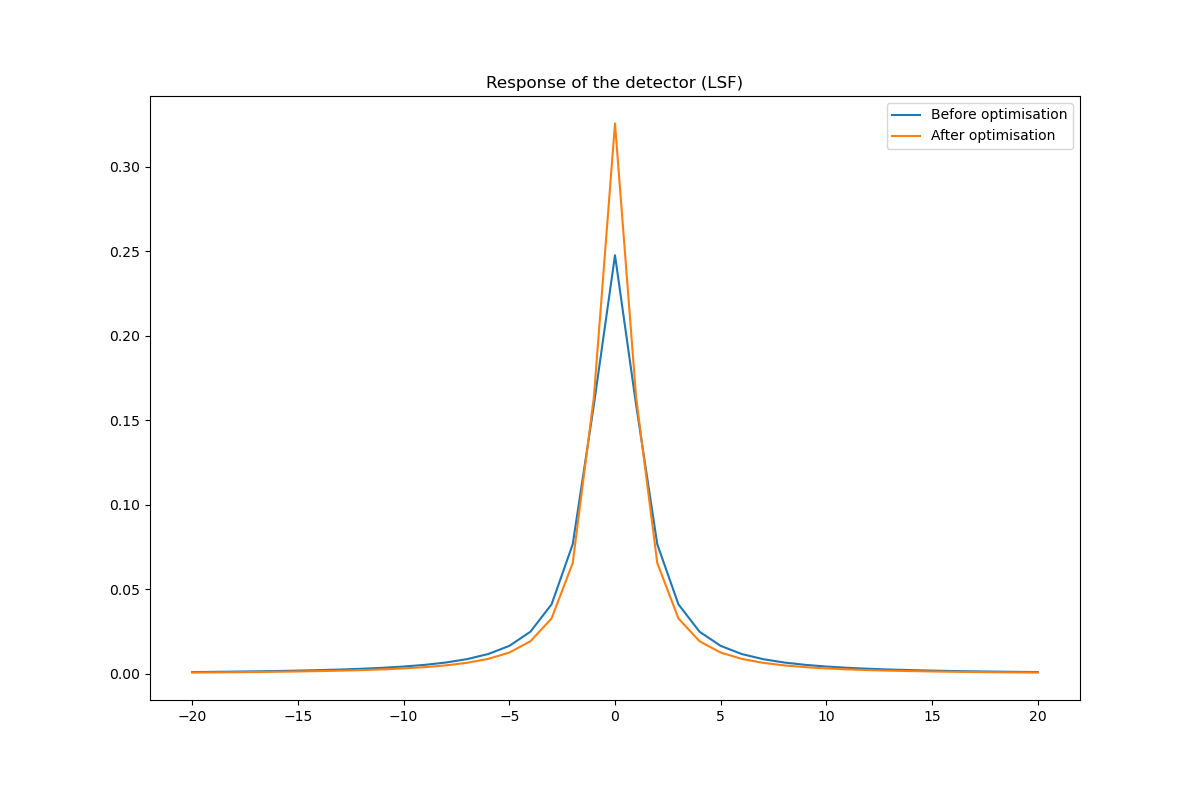
\includegraphics{plots/LSF_optimised.png}
\caption{Response of the detector (LSF)}
\end{figure}

\hypertarget{extract-the-fibre-in-the-centre-of-the-ct-slices}{%
\subsection{Extract the fibre in the centre of the CT
slices}\label{extract-the-fibre-in-the-centre-of-the-ct-slices}}

    \begin{tcolorbox}[breakable, size=fbox, boxrule=1pt, pad at break*=1mm,colback=cellbackground, colframe=cellborder]
\prompt{In}{incolor}{89}{\boxspacing}
\begin{Verbatim}[commandchars=\\\{\}]
\PY{k}{def} \PY{n+nf}{findFibreInCentreOfCtSlice}\PY{p}{(}\PY{p}{)}\PY{p}{:}
    \PY{k}{global} \PY{n}{centroid\PYZus{}set}\PY{p}{;}
    \PY{k}{global} \PY{n}{reference\PYZus{}CT}\PY{p}{;}
    \PY{k}{global} \PY{n}{cylinder\PYZus{}position\PYZus{}in\PYZus{}centre\PYZus{}of\PYZus{}slice}\PY{p}{;}

    \PY{c+c1}{\PYZsh{} Find the cylinder in the centre of the image}
    \PY{n}{cylinder\PYZus{}position\PYZus{}in\PYZus{}centre\PYZus{}of\PYZus{}slice} \PY{o}{=} \PY{k+kc}{None}\PY{p}{;}
    \PY{n}{best\PYZus{}distance} \PY{o}{=} \PY{n}{sys}\PY{o}{.}\PY{n}{float\PYZus{}info}\PY{o}{.}\PY{n}{max}\PY{p}{;}

    \PY{k}{for} \PY{n}{centre} \PY{o+ow}{in} \PY{n}{centroid\PYZus{}set}\PY{p}{:}
        \PY{n}{distance} \PY{o}{=} \PY{n}{math}\PY{o}{.}\PY{n}{pow}\PY{p}{(}\PY{n}{centre}\PY{p}{[}\PY{l+m+mi}{0}\PY{p}{]} \PY{o}{\PYZhy{}} \PY{n}{reference\PYZus{}CT}\PY{o}{.}\PY{n}{shape}\PY{p}{[}\PY{l+m+mi}{1}\PY{p}{]} \PY{o}{/} \PY{l+m+mi}{2}\PY{p}{,}\PY{l+m+mi}{2} \PY{p}{)} \PY{o}{+} \PY{n}{math}\PY{o}{.}\PY{n}{pow}\PY{p}{(}\PY{n}{centre}\PY{p}{[}\PY{l+m+mi}{1}\PY{p}{]} \PY{o}{\PYZhy{}} \PY{n}{reference\PYZus{}CT}\PY{o}{.}\PY{n}{shape}\PY{p}{[}\PY{l+m+mi}{0}\PY{p}{]} \PY{o}{/} \PY{l+m+mi}{2}\PY{p}{,} \PY{l+m+mi}{2}\PY{p}{)}\PY{p}{;}

        \PY{k}{if} \PY{n}{best\PYZus{}distance} \PY{o}{\PYZgt{}} \PY{n}{distance}\PY{p}{:}
            \PY{n}{best\PYZus{}distance} \PY{o}{=} \PY{n}{distance}\PY{p}{;}
            \PY{n}{cylinder\PYZus{}position\PYZus{}in\PYZus{}centre\PYZus{}of\PYZus{}slice} \PY{o}{=} \PY{n}{copy}\PY{o}{.}\PY{n}{deepcopy}\PY{p}{(}\PY{n}{centre}\PY{p}{)}\PY{p}{;}

    \PY{k}{return} \PY{n}{cylinder\PYZus{}position\PYZus{}in\PYZus{}centre\PYZus{}of\PYZus{}slice}\PY{p}{;}
\end{Verbatim}
\end{tcolorbox}

    \begin{tcolorbox}[breakable, size=fbox, boxrule=1pt, pad at break*=1mm,colback=cellbackground, colframe=cellborder]
\prompt{In}{incolor}{90}{\boxspacing}
\begin{Verbatim}[commandchars=\\\{\}]
\PY{n}{findFibreInCentreOfCtSlice}\PY{p}{(}\PY{p}{)}\PY{p}{;}

\PY{n}{reference\PYZus{}fibre\PYZus{}in\PYZus{}centre} \PY{o}{=} \PY{n}{np}\PY{o}{.}\PY{n}{array}\PY{p}{(}\PY{n}{copy}\PY{o}{.}\PY{n}{deepcopy}\PY{p}{(}\PY{n}{reference\PYZus{}CT}\PY{p}{[}\PY{n}{cylinder\PYZus{}position\PYZus{}in\PYZus{}centre\PYZus{}of\PYZus{}slice}\PY{p}{[}\PY{l+m+mi}{1}\PY{p}{]} \PY{o}{\PYZhy{}} \PY{n}{roi\PYZus{}length}\PY{p}{:}\PY{n}{cylinder\PYZus{}position\PYZus{}in\PYZus{}centre\PYZus{}of\PYZus{}slice}\PY{p}{[}\PY{l+m+mi}{1}\PY{p}{]} \PY{o}{+} \PY{n}{roi\PYZus{}length}\PY{p}{,} \PY{n}{cylinder\PYZus{}position\PYZus{}in\PYZus{}centre\PYZus{}of\PYZus{}slice}\PY{p}{[}\PY{l+m+mi}{0}\PY{p}{]} \PY{o}{\PYZhy{}} \PY{n}{roi\PYZus{}length}\PY{p}{:}\PY{n}{cylinder\PYZus{}position\PYZus{}in\PYZus{}centre\PYZus{}of\PYZus{}slice}\PY{p}{[}\PY{l+m+mi}{0}\PY{p}{]} \PY{o}{+} \PY{n}{roi\PYZus{}length}\PY{p}{]}\PY{p}{)}\PY{p}{)}\PY{p}{;}
\PY{n}{test\PYZus{}fibre\PYZus{}in\PYZus{}centre}      \PY{o}{=} \PY{n}{np}\PY{o}{.}\PY{n}{array}\PY{p}{(}\PY{n}{copy}\PY{o}{.}\PY{n}{deepcopy}\PY{p}{(}\PY{n}{simulated\PYZus{}CT}\PY{p}{[}\PY{n}{cylinder\PYZus{}position\PYZus{}in\PYZus{}centre\PYZus{}of\PYZus{}slice}\PY{p}{[}\PY{l+m+mi}{1}\PY{p}{]} \PY{o}{\PYZhy{}} \PY{n}{roi\PYZus{}length}\PY{p}{:}\PY{n}{cylinder\PYZus{}position\PYZus{}in\PYZus{}centre\PYZus{}of\PYZus{}slice}\PY{p}{[}\PY{l+m+mi}{1}\PY{p}{]} \PY{o}{+} \PY{n}{roi\PYZus{}length}\PY{p}{,} \PY{n}{cylinder\PYZus{}position\PYZus{}in\PYZus{}centre\PYZus{}of\PYZus{}slice}\PY{p}{[}\PY{l+m+mi}{0}\PY{p}{]} \PY{o}{\PYZhy{}} \PY{n}{roi\PYZus{}length}\PY{p}{:}\PY{n}{cylinder\PYZus{}position\PYZus{}in\PYZus{}centre\PYZus{}of\PYZus{}slice}\PY{p}{[}\PY{l+m+mi}{0}\PY{p}{]} \PY{o}{+} \PY{n}{roi\PYZus{}length}\PY{p}{]}\PY{p}{)}\PY{p}{)}\PY{p}{;}

\PY{n}{profile\PYZus{}reference} \PY{o}{=} \PY{n}{copy}\PY{o}{.}\PY{n}{deepcopy}\PY{p}{(}\PY{n}{np}\PY{o}{.}\PY{n}{diag}\PY{p}{(}\PY{n}{reference\PYZus{}fibre\PYZus{}in\PYZus{}centre}\PY{p}{)}\PY{p}{)}\PY{p}{;}
\PY{n}{profile\PYZus{}test\PYZus{}without\PYZus{}Poisson\PYZus{}noise} \PY{o}{=} \PY{n}{copy}\PY{o}{.}\PY{n}{deepcopy}\PY{p}{(}\PY{n}{np}\PY{o}{.}\PY{n}{diag}\PY{p}{(}\PY{n}{test\PYZus{}fibre\PYZus{}in\PYZus{}centre}\PY{p}{)}\PY{p}{)}\PY{p}{;}

\PY{n}{reference\PYZus{}fibre\PYZus{}in\PYZus{}centre} \PY{o}{=} \PY{n}{standardisation}\PY{p}{(}\PY{n}{reference\PYZus{}fibre\PYZus{}in\PYZus{}centre}\PY{p}{)}\PY{p}{;}
\PY{n}{test\PYZus{}fibre\PYZus{}in\PYZus{}centre} \PY{o}{=} \PY{n}{standardisation}\PY{p}{(}\PY{n}{test\PYZus{}fibre\PYZus{}in\PYZus{}centre}\PY{p}{)}\PY{p}{;}
\end{Verbatim}
\end{tcolorbox}

    \begin{tcolorbox}[breakable, size=fbox, boxrule=1pt, pad at break*=1mm,colback=cellbackground, colframe=cellborder]
\prompt{In}{incolor}{91}{\boxspacing}
\begin{Verbatim}[commandchars=\\\{\}]
\PY{n}{norm} \PY{o}{=} \PY{n}{cm}\PY{o}{.}\PY{n}{colors}\PY{o}{.}\PY{n}{Normalize}\PY{p}{(}\PY{n}{vmax}\PY{o}{=}\PY{l+m+mf}{1.25}\PY{p}{,} \PY{n}{vmin}\PY{o}{=}\PY{o}{\PYZhy{}}\PY{l+m+mf}{0.5}\PY{p}{)}

\PY{n}{fig}\PY{p}{,} \PY{p}{(}\PY{n}{ax1}\PY{p}{,} \PY{n}{ax2}\PY{p}{,} \PY{n}{ax3}\PY{p}{)} \PY{o}{=} \PY{n}{plt}\PY{o}{.}\PY{n}{subplots}\PY{p}{(}\PY{l+m+mi}{1}\PY{p}{,} \PY{l+m+mi}{3}\PY{p}{)}
\PY{n}{plt}\PY{o}{.}\PY{n}{tight\PYZus{}layout}\PY{p}{(}\PY{p}{)}
\PY{n}{fig}\PY{o}{.}\PY{n}{suptitle}\PY{p}{(}\PY{l+s+s1}{\PYZsq{}}\PY{l+s+s1}{Fibre in the centre of the CT slices}\PY{l+s+s1}{\PYZsq{}}\PY{p}{)}

\PY{n}{ax1}\PY{o}{.}\PY{n}{set\PYZus{}title}\PY{p}{(}\PY{l+s+s2}{\PYZdq{}}\PY{l+s+s2}{Reference image}\PY{l+s+s2}{\PYZdq{}}\PY{p}{)}\PY{p}{;}
\PY{n}{imgplot1} \PY{o}{=} \PY{n}{ax1}\PY{o}{.}\PY{n}{imshow}\PY{p}{(}\PY{n}{reference\PYZus{}fibre\PYZus{}in\PYZus{}centre}\PY{p}{,} \PY{n}{cmap}\PY{o}{=}\PY{l+s+s2}{\PYZdq{}}\PY{l+s+s2}{gray}\PY{l+s+s2}{\PYZdq{}}\PY{p}{,} 
                     \PY{n}{norm}\PY{o}{=}\PY{n}{norm}\PY{p}{)}\PY{p}{;}

\PY{n}{ax2}\PY{o}{.}\PY{n}{set\PYZus{}title}\PY{p}{(}\PY{l+s+s2}{\PYZdq{}}\PY{l+s+s2}{Simulated CT slice after automatic registration}\PY{l+s+s2}{\PYZdq{}}\PY{p}{)}\PY{p}{;}
\PY{n}{imgplot2} \PY{o}{=} \PY{n}{ax2}\PY{o}{.}\PY{n}{imshow}\PY{p}{(}\PY{n}{test\PYZus{}fibre\PYZus{}in\PYZus{}centre}\PY{p}{,}
                     \PY{n}{cmap}\PY{o}{=}\PY{l+s+s1}{\PYZsq{}}\PY{l+s+s1}{gray}\PY{l+s+s1}{\PYZsq{}}\PY{p}{,}
                     \PY{n}{norm}\PY{o}{=}\PY{n}{norm}\PY{p}{)}\PY{p}{;}

\PY{n}{comp\PYZus{}equalized} \PY{o}{=} \PY{n}{compare\PYZus{}images}\PY{p}{(}\PY{n}{reference\PYZus{}fibre\PYZus{}in\PYZus{}centre}\PY{p}{,} \PY{n}{test\PYZus{}fibre\PYZus{}in\PYZus{}centre}\PY{p}{,} \PY{n}{method}\PY{o}{=}\PY{l+s+s1}{\PYZsq{}}\PY{l+s+s1}{checkerboard}\PY{l+s+s1}{\PYZsq{}}\PY{p}{)}\PY{p}{;}
\PY{n}{ax3}\PY{o}{.}\PY{n}{set\PYZus{}title}\PY{p}{(}\PY{l+s+s2}{\PYZdq{}}\PY{l+s+s2}{Checkboard comparison between}\PY{l+s+se}{\PYZbs{}n}\PY{l+s+s2}{\PYZdq{}} \PY{o}{+} 
              \PY{l+s+s2}{\PYZdq{}}\PY{l+s+s2}{the reference and simulated images}\PY{l+s+se}{\PYZbs{}n}\PY{l+s+s2}{ZNCC: }\PY{l+s+s2}{\PYZdq{}} \PY{o}{+} 
              \PY{l+s+s2}{\PYZdq{}}\PY{l+s+si}{\PYZob{}:.2f\PYZcb{}}\PY{l+s+s2}{\PYZdq{}}\PY{o}{.}\PY{n}{format}\PY{p}{(}\PY{l+m+mf}{100.0} \PY{o}{*} \PY{n}{np}\PY{o}{.}\PY{n}{mean}\PY{p}{(}\PY{n}{np}\PY{o}{.}\PY{n}{multiply}\PY{p}{(}\PY{n}{reference\PYZus{}fibre\PYZus{}in\PYZus{}centre}\PY{p}{,} \PY{n}{test\PYZus{}fibre\PYZus{}in\PYZus{}centre}\PY{p}{)}\PY{p}{)}\PY{p}{)}\PY{p}{)}\PY{p}{;}
\PY{n}{imgplot3} \PY{o}{=} \PY{n}{ax3}\PY{o}{.}\PY{n}{imshow}\PY{p}{(}\PY{n}{comp\PYZus{}equalized}\PY{p}{,}
                     \PY{n}{cmap}\PY{o}{=}\PY{l+s+s1}{\PYZsq{}}\PY{l+s+s1}{gray}\PY{l+s+s1}{\PYZsq{}}\PY{p}{,}
                     \PY{n}{norm}\PY{o}{=}\PY{n}{norm}\PY{p}{)}\PY{p}{;}

\PY{n}{plt}\PY{o}{.}\PY{n}{savefig}\PY{p}{(}\PY{l+s+s1}{\PYZsq{}}\PY{l+s+s1}{plots/Fibre\PYZus{}in\PYZus{}centre\PYZus{}CT\PYZus{}slices\PYZus{}before\PYZus{}noise.pdf}\PY{l+s+s1}{\PYZsq{}}\PY{p}{)}\PY{p}{;}
\PY{n}{plt}\PY{o}{.}\PY{n}{savefig}\PY{p}{(}\PY{l+s+s1}{\PYZsq{}}\PY{l+s+s1}{plots/Fibre\PYZus{}in\PYZus{}centre\PYZus{}CT\PYZus{}slices\PYZus{}before\PYZus{}noise.png}\PY{l+s+s1}{\PYZsq{}}\PY{p}{)}\PY{p}{;}
\end{Verbatim}
\end{tcolorbox}

    \begin{figure}
\centering
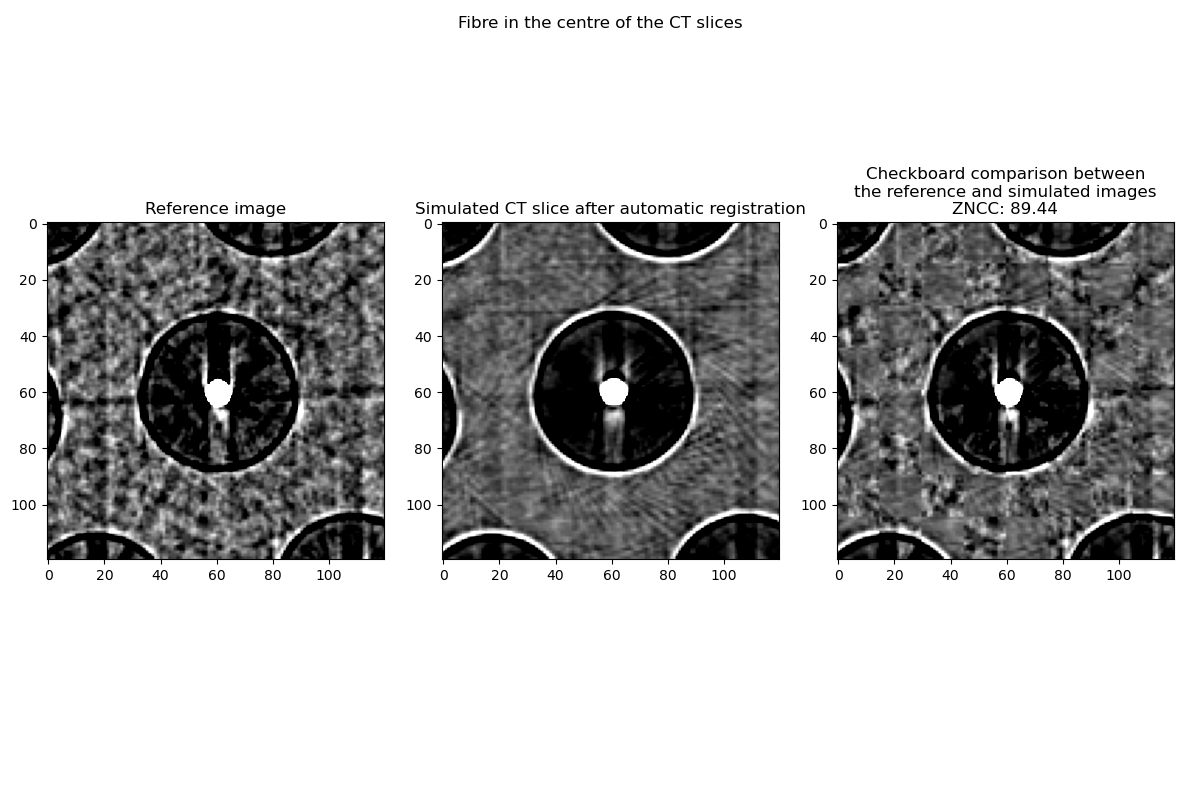
\includegraphics{plots/Fibre_in_centre_CT_slices_before_noise.png}
\caption{Fibre in the centre of the CT slices}
\end{figure}

    \hypertarget{optimisation-of-the-poisson-noise}{%
\section{Optimisation of the Poisson
noise}\label{optimisation-of-the-poisson-noise}}

    \begin{tcolorbox}[breakable, size=fbox, boxrule=1pt, pad at break*=1mm,colback=cellbackground, colframe=cellborder]
\prompt{In}{incolor}{92}{\boxspacing}
\begin{Verbatim}[commandchars=\\\{\}]
\PY{k}{def} \PY{n+nf}{fitnessFunctionNoise}\PY{p}{(}\PY{n}{x}\PY{p}{)}\PY{p}{:}
    \PY{k}{global} \PY{n}{best\PYZus{}fitness}\PY{p}{;}
    \PY{k}{global} \PY{n}{best\PYZus{}fitness\PYZus{}id}\PY{p}{;}
    \PY{k}{global} \PY{n}{prefix}\PY{p}{;}
    
    \PY{n}{bias} \PY{o}{=} \PY{n}{x}\PY{p}{[}\PY{l+m+mi}{0}\PY{p}{]}\PY{p}{;}
    \PY{n}{gain} \PY{o}{=} \PY{n}{x}\PY{p}{[}\PY{l+m+mi}{1}\PY{p}{]}\PY{p}{;}
    \PY{n}{scale} \PY{o}{=} \PY{n}{x}\PY{p}{[}\PY{l+m+mi}{2}\PY{p}{]}\PY{p}{;}

    \PY{c+c1}{\PYZsh{} Poisson noise}
    \PY{n+nb}{map} \PY{o}{=} \PY{p}{(}\PY{n}{normalised\PYZus{}projections\PYZus{}ROI} \PY{o}{+} \PY{p}{(}\PY{n}{bias} \PY{o}{+} \PY{l+m+mi}{1}\PY{p}{)}\PY{p}{)} \PY{o}{*} \PY{n}{gain}\PY{p}{;}
    \PY{n}{temp} \PY{o}{=} \PY{n}{np}\PY{o}{.}\PY{n}{random}\PY{o}{.}\PY{n}{poisson}\PY{p}{(}\PY{n+nb}{map}\PY{p}{)}\PY{o}{.}\PY{n}{astype}\PY{p}{(}\PY{n+nb}{float}\PY{p}{)}\PY{p}{;}
    \PY{n}{temp} \PY{o}{/}\PY{o}{=} \PY{n}{gain}\PY{p}{;}
    \PY{n}{temp} \PY{o}{\PYZhy{}}\PY{o}{=} \PY{n}{bias} \PY{o}{+} \PY{l+m+mi}{1}\PY{p}{;}
    
    \PY{c+c1}{\PYZsh{} Noise map}
    \PY{n}{noise\PYZus{}map} \PY{o}{=} \PY{n}{normalised\PYZus{}projections\PYZus{}ROI} \PY{o}{\PYZhy{}} \PY{n}{temp}\PY{p}{;}
    \PY{n}{noise\PYZus{}map} \PY{o}{*}\PY{o}{=} \PY{n}{scale}\PY{p}{;}
    \PY{n}{noisy\PYZus{}image} \PY{o}{=} \PY{n}{normalised\PYZus{}projections\PYZus{}ROI} \PY{o}{+} \PY{n}{noise\PYZus{}map}\PY{p}{;}

    \PY{c+c1}{\PYZsh{} Compute the standard deviation of the pixel values in the ROI extracted from the simulated image with noise}
    \PY{n}{noisy\PYZus{}image\PYZus{}noise\PYZus{}ROI\PYZus{}stddev} \PY{o}{=} \PY{l+m+mi}{0}\PY{p}{;}
    \PY{k}{for} \PY{n}{y} \PY{o+ow}{in} \PY{n+nb}{range}\PY{p}{(}\PY{n}{noisy\PYZus{}image}\PY{o}{.}\PY{n}{shape}\PY{p}{[}\PY{l+m+mi}{0}\PY{p}{]}\PY{p}{)}\PY{p}{:}
        \PY{n}{noisy\PYZus{}image\PYZus{}noise\PYZus{}ROI\PYZus{}stddev} \PY{o}{+}\PY{o}{=} \PY{n}{noisy\PYZus{}image}\PY{p}{[}\PY{n}{y}\PY{p}{]}\PY{o}{.}\PY{n}{std}\PY{p}{(}\PY{p}{)}\PY{p}{;}
    \PY{n}{noisy\PYZus{}image\PYZus{}noise\PYZus{}ROI\PYZus{}stddev} \PY{o}{/}\PY{o}{=} \PY{n}{noisy\PYZus{}image}\PY{o}{.}\PY{n}{shape}\PY{p}{[}\PY{l+m+mi}{0}\PY{p}{]}\PY{p}{;}

    \PY{c+c1}{\PYZsh{} Difference of std dev between the reference and the simulated image}
    \PY{n}{diff} \PY{o}{=} \PY{n}{reference\PYZus{}noise\PYZus{}ROI\PYZus{}stddev} \PY{o}{\PYZhy{}} \PY{n}{noisy\PYZus{}image\PYZus{}noise\PYZus{}ROI\PYZus{}stddev}\PY{p}{;}
    \PY{n}{objective} \PY{o}{=} \PY{n}{diff} \PY{o}{*} \PY{n}{diff}\PY{p}{;}
    
    \PY{c+c1}{\PYZsh{} The block below is not necessary for the registration.}
    \PY{c+c1}{\PYZsh{} It is used to save the data to create animations.}
    \PY{k}{if} \PY{n}{best\PYZus{}fitness} \PY{o}{\PYZgt{}} \PY{n}{objective}\PY{p}{:}
        \PY{n}{best\PYZus{}fitness} \PY{o}{=} \PY{n}{objective}\PY{p}{;}
    
        \PY{c+c1}{\PYZsh{} Save the simulated CT slice}
        \PY{n}{saveMHA}\PY{p}{(}\PY{l+s+s2}{\PYZdq{}}\PY{l+s+s2}{outputs/}\PY{l+s+s2}{\PYZdq{}} \PY{o}{+} \PY{n}{prefix} \PY{o}{+} \PY{l+s+s2}{\PYZdq{}}\PY{l+s+s2}{noisy\PYZus{}image\PYZus{}}\PY{l+s+s2}{\PYZdq{}} \PY{o}{+} \PY{n+nb}{str}\PY{p}{(}\PY{n}{best\PYZus{}fitness\PYZus{}id}\PY{p}{)} \PY{o}{+} \PY{l+s+s2}{\PYZdq{}}\PY{l+s+s2}{.mha}\PY{l+s+s2}{\PYZdq{}}\PY{p}{,}
                \PY{n}{noisy\PYZus{}image}\PY{p}{,}
                \PY{p}{[}\PY{n}{pixel\PYZus{}spacing\PYZus{}in\PYZus{}mm}\PY{p}{,} \PY{n}{pixel\PYZus{}spacing\PYZus{}in\PYZus{}mm}\PY{p}{,} \PY{n}{pixel\PYZus{}spacing\PYZus{}in\PYZus{}mm}\PY{p}{]}\PY{p}{)}\PY{p}{;}

        \PY{n}{np}\PY{o}{.}\PY{n}{savetxt}\PY{p}{(}\PY{l+s+s2}{\PYZdq{}}\PY{l+s+s2}{outputs/}\PY{l+s+s2}{\PYZdq{}} \PY{o}{+} \PY{n}{prefix} \PY{o}{+} \PY{n+nb}{str}\PY{p}{(}\PY{n}{best\PYZus{}fitness\PYZus{}id}\PY{p}{)} \PY{o}{+} \PY{l+s+s2}{\PYZdq{}}\PY{l+s+s2}{.dat}\PY{l+s+s2}{\PYZdq{}}\PY{p}{,} \PY{p}{[}\PY{n}{bias}\PY{p}{,} \PY{n}{gain}\PY{p}{,} \PY{n}{scale}\PY{p}{]}\PY{p}{,} \PY{n}{header}\PY{o}{=}\PY{l+s+s1}{\PYZsq{}}\PY{l+s+s1}{bias, gain, scale}\PY{l+s+s1}{\PYZsq{}}\PY{p}{)}\PY{p}{;}
        
        \PY{n}{best\PYZus{}fitness\PYZus{}id} \PY{o}{+}\PY{o}{=} \PY{l+m+mi}{1}\PY{p}{;}

    \PY{k}{return} \PY{n}{objective}
\end{Verbatim}
\end{tcolorbox}

    \begin{tcolorbox}[breakable, size=fbox, boxrule=1pt, pad at break*=1mm,colback=cellbackground, colframe=cellborder]
\prompt{In}{incolor}{93}{\boxspacing}
\begin{Verbatim}[commandchars=\\\{\}]
\PY{c+c1}{\PYZsh{} The registration has already been performed. Load the results.}
\PY{k}{if} \PY{n}{os}\PY{o}{.}\PY{n}{path}\PY{o}{.}\PY{n}{isfile}\PY{p}{(}\PY{l+s+s2}{\PYZdq{}}\PY{l+s+s2}{outputs/poisson\PYZhy{}noise.dat}\PY{l+s+s2}{\PYZdq{}}\PY{p}{)}\PY{p}{:}
    \PY{n}{temp} \PY{o}{=} \PY{n}{np}\PY{o}{.}\PY{n}{loadtxt}\PY{p}{(}\PY{l+s+s2}{\PYZdq{}}\PY{l+s+s2}{outputs/poisson\PYZhy{}noise.dat}\PY{l+s+s2}{\PYZdq{}}\PY{p}{)}\PY{p}{;}
    \PY{n}{bias} \PY{o}{=} \PY{n}{temp}\PY{p}{[}\PY{l+m+mi}{0}\PY{p}{]}\PY{p}{;}
    \PY{n}{gain} \PY{o}{=} \PY{n}{temp}\PY{p}{[}\PY{l+m+mi}{1}\PY{p}{]}\PY{p}{;}
    \PY{n}{scale} \PY{o}{=} \PY{n}{temp}\PY{p}{[}\PY{l+m+mi}{2}\PY{p}{]}\PY{p}{;}

\PY{c+c1}{\PYZsh{} Perform the registration using CMA\PYZhy{}ES}
\PY{k}{else}\PY{p}{:}

    \PY{c+c1}{\PYZsh{} Extract a ROI from the reference where no object is}
    \PY{n}{reference\PYZus{}noise\PYZus{}ROI} \PY{o}{=} \PY{n}{copy}\PY{o}{.}\PY{n}{deepcopy}\PY{p}{(}\PY{n}{reference\PYZus{}normalised\PYZus{}projections}\PY{p}{[}\PY{l+m+mi}{450}\PY{p}{:}\PY{l+m+mi}{550}\PY{p}{,}\PY{l+m+mi}{0}\PY{p}{:}\PY{l+m+mi}{125}\PY{p}{]}\PY{p}{)}\PY{p}{;}

    \PY{n}{saveMHA}\PY{p}{(}\PY{l+s+s2}{\PYZdq{}}\PY{l+s+s2}{outputs/reference\PYZus{}noise\PYZus{}ROI.mha}\PY{l+s+s2}{\PYZdq{}}\PY{p}{,}
           \PY{n}{reference\PYZus{}noise\PYZus{}ROI}\PY{p}{,}
           \PY{p}{[}\PY{n}{pixel\PYZus{}spacing\PYZus{}in\PYZus{}mm}\PY{p}{,} \PY{n}{angular\PYZus{}step}\PY{p}{,} \PY{n}{pixel\PYZus{}spacing\PYZus{}in\PYZus{}mm}\PY{p}{]}\PY{p}{)}\PY{p}{;}

    \PY{c+c1}{\PYZsh{} Compute the standard deviation of the pixel values in the ROI extracted from the reference}
    \PY{n}{reference\PYZus{}noise\PYZus{}ROI\PYZus{}stddev} \PY{o}{=} \PY{l+m+mi}{0}\PY{p}{;}
    \PY{k}{for} \PY{n}{y} \PY{o+ow}{in} \PY{n+nb}{range}\PY{p}{(}\PY{n}{reference\PYZus{}noise\PYZus{}ROI}\PY{o}{.}\PY{n}{shape}\PY{p}{[}\PY{l+m+mi}{0}\PY{p}{]}\PY{p}{)}\PY{p}{:}
        \PY{n}{reference\PYZus{}noise\PYZus{}ROI\PYZus{}stddev} \PY{o}{+}\PY{o}{=} \PY{n}{reference\PYZus{}noise\PYZus{}ROI}\PY{p}{[}\PY{n}{y}\PY{p}{]}\PY{o}{.}\PY{n}{std}\PY{p}{(}\PY{p}{)}\PY{p}{;}
    \PY{n}{reference\PYZus{}noise\PYZus{}ROI\PYZus{}stddev} \PY{o}{/}\PY{o}{=} \PY{n}{reference\PYZus{}noise\PYZus{}ROI}\PY{o}{.}\PY{n}{shape}\PY{p}{[}\PY{l+m+mi}{0}\PY{p}{]}\PY{p}{;}

    \PY{c+c1}{\PYZsh{} Copy the simulated projection in a temporary variable}
    \PY{n}{temp} \PY{o}{=} \PY{n}{copy}\PY{o}{.}\PY{n}{deepcopy}\PY{p}{(}\PY{n}{normalised\PYZus{}projections}\PY{p}{)}\PY{p}{;}
    \PY{n}{temp}\PY{o}{.}\PY{n}{shape} \PY{o}{=} \PY{n}{reference\PYZus{}normalised\PYZus{}projections}\PY{o}{.}\PY{n}{shape}

    \PY{c+c1}{\PYZsh{} Extract the corresponding ROI}
    \PY{n}{normalised\PYZus{}projections\PYZus{}ROI} \PY{o}{=} \PY{n}{temp}\PY{p}{[}\PY{l+m+mi}{450}\PY{p}{:}\PY{l+m+mi}{550}\PY{p}{,}\PY{l+m+mi}{0}\PY{p}{:}\PY{l+m+mi}{125}\PY{p}{]}\PY{p}{;}

    \PY{n}{saveMHA}\PY{p}{(}\PY{l+s+s2}{\PYZdq{}}\PY{l+s+s2}{outputs/normalised\PYZus{}projections\PYZus{}ROI.mha}\PY{l+s+s2}{\PYZdq{}}\PY{p}{,}
           \PY{n}{normalised\PYZus{}projections\PYZus{}ROI}\PY{p}{,}
           \PY{p}{[}\PY{n}{pixel\PYZus{}spacing\PYZus{}in\PYZus{}mm}\PY{p}{,} \PY{n}{angular\PYZus{}step}\PY{p}{,} \PY{n}{pixel\PYZus{}spacing\PYZus{}in\PYZus{}mm}\PY{p}{]}\PY{p}{)}\PY{p}{;}
    
    \PY{c+c1}{\PYZsh{} Initialise the values}
    \PY{n}{bias} \PY{o}{=} \PY{l+m+mf}{0.0}\PY{p}{;}
    \PY{n}{gain} \PY{o}{=} \PY{l+m+mf}{255.0}\PY{p}{;}
    \PY{n}{scale} \PY{o}{=} \PY{l+m+mi}{1}\PY{p}{;}

    \PY{n}{x0} \PY{o}{=} \PY{p}{[}\PY{n}{bias}\PY{p}{,} \PY{n}{gain}\PY{p}{,} \PY{n}{scale}\PY{p}{]}\PY{p}{;}

    \PY{n}{bounds} \PY{o}{=} \PY{p}{[}
        \PY{p}{[}\PY{o}{\PYZhy{}}\PY{l+m+mf}{1.0}\PY{p}{,}   \PY{l+m+mf}{0.0}\PY{p}{,} \PY{l+m+mf}{0.0}\PY{p}{]}\PY{p}{,}
        \PY{p}{[} \PY{l+m+mf}{5.0}\PY{p}{,} \PY{l+m+mf}{255.0}\PY{p}{,} \PY{l+m+mf}{255.0}\PY{p}{]}
    \PY{p}{]}\PY{p}{;}

    \PY{n}{opts} \PY{o}{=} \PY{n}{cma}\PY{o}{.}\PY{n}{CMAOptions}\PY{p}{(}\PY{p}{)}
    \PY{n}{opts}\PY{o}{.}\PY{n}{set}\PY{p}{(}\PY{l+s+s1}{\PYZsq{}}\PY{l+s+s1}{tolfun}\PY{l+s+s1}{\PYZsq{}}\PY{p}{,} \PY{l+m+mf}{1e\PYZhy{}8}\PY{p}{)}\PY{p}{;}
    \PY{n}{opts}\PY{p}{[}\PY{l+s+s1}{\PYZsq{}}\PY{l+s+s1}{tolx}\PY{l+s+s1}{\PYZsq{}}\PY{p}{]} \PY{o}{=} \PY{l+m+mf}{1e\PYZhy{}8}\PY{p}{;}
    \PY{n}{opts}\PY{p}{[}\PY{l+s+s1}{\PYZsq{}}\PY{l+s+s1}{bounds}\PY{l+s+s1}{\PYZsq{}}\PY{p}{]} \PY{o}{=} \PY{n}{bounds}\PY{p}{;}
    \PY{n}{opts}\PY{p}{[}\PY{l+s+s1}{\PYZsq{}}\PY{l+s+s1}{CMA\PYZus{}stds}\PY{l+s+s1}{\PYZsq{}}\PY{p}{]} \PY{o}{=} \PY{p}{[}\PY{l+m+mi}{1}\PY{p}{,} \PY{l+m+mi}{10}\PY{p}{,} \PY{l+m+mi}{10}\PY{p}{]}\PY{p}{;}

    \PY{n}{best\PYZus{}fitness} \PY{o}{=} \PY{n}{sys}\PY{o}{.}\PY{n}{float\PYZus{}info}\PY{o}{.}\PY{n}{max}\PY{p}{;}
    \PY{n}{best\PYZus{}fitness\PYZus{}id} \PY{o}{=} \PY{l+m+mi}{0}\PY{p}{;}
    \PY{n}{prefix} \PY{o}{=} \PY{l+s+s2}{\PYZdq{}}\PY{l+s+s2}{poisson\PYZhy{}noise\PYZus{}}\PY{l+s+s2}{\PYZdq{}}\PY{p}{;}

    \PY{n}{es} \PY{o}{=} \PY{n}{cma}\PY{o}{.}\PY{n}{CMAEvolutionStrategy}\PY{p}{(}\PY{n}{x0}\PY{p}{,} \PY{l+m+mf}{0.25}\PY{p}{,} \PY{n}{opts}\PY{p}{)}\PY{p}{;}
    \PY{n}{es}\PY{o}{.}\PY{n}{optimize}\PY{p}{(}\PY{n}{fitnessFunctionNoise}\PY{p}{)}\PY{p}{;}

    \PY{n}{bias} \PY{o}{=} \PY{n}{es}\PY{o}{.}\PY{n}{result}\PY{o}{.}\PY{n}{xbest}\PY{p}{[}\PY{l+m+mi}{0}\PY{p}{]}\PY{p}{;}
    \PY{n}{gain} \PY{o}{=} \PY{n}{es}\PY{o}{.}\PY{n}{result}\PY{o}{.}\PY{n}{xbest}\PY{p}{[}\PY{l+m+mi}{1}\PY{p}{]}\PY{p}{;}
    \PY{n}{scale} \PY{o}{=} \PY{n}{es}\PY{o}{.}\PY{n}{result}\PY{o}{.}\PY{n}{xbest}\PY{p}{[}\PY{l+m+mi}{2}\PY{p}{]}\PY{p}{;}

    \PY{n}{np}\PY{o}{.}\PY{n}{savetxt}\PY{p}{(}\PY{l+s+s2}{\PYZdq{}}\PY{l+s+s2}{outputs/poisson\PYZhy{}noise.dat}\PY{l+s+s2}{\PYZdq{}}\PY{p}{,} \PY{p}{[}\PY{n}{bias}\PY{p}{,} \PY{n}{gain}\PY{p}{,} \PY{n}{scale}\PY{p}{]}\PY{p}{,} \PY{n}{header}\PY{o}{=}\PY{l+s+s1}{\PYZsq{}}\PY{l+s+s1}{bias, gain, scale}\PY{l+s+s1}{\PYZsq{}}\PY{p}{)}\PY{p}{;}
    
    \PY{c+c1}{\PYZsh{} Release memory}
    \PY{k}{del} \PY{n}{es}\PY{p}{;}
\end{Verbatim}
\end{tcolorbox}

    \begin{Verbatim}[commandchars=\\\{\}]
(3\_w,7)-aCMA-ES (mu\_w=2.3,w\_1=58\%) in dimension 3 (seed=274415, Tue Jun  8
21:50:49 2021)
Iterat \#Fevals   function value  axis ratio  sigma  min\&max std  t[m:s]
    1      7 1.267864360255033e-06 1.0e+00 2.49e-01  2e-01  3e+00 0:00.0
    2     14 7.069104818027832e-03 1.3e+00 2.51e-01  2e-01  3e+00 0:00.0
    3     21 1.898353300214850e-05 1.6e+00 2.52e-01  2e-01  3e+00 0:00.0
   68    476 1.557615628674367e-10 2.8e+03 4.43e-02  8e-04  7e-01 0:01.1
    \end{Verbatim}

    \begin{tcolorbox}[breakable, size=fbox, boxrule=1pt, pad at break*=1mm,colback=cellbackground, colframe=cellborder]
\prompt{In}{incolor}{94}{\boxspacing}
\begin{Verbatim}[commandchars=\\\{\}]
\PY{n+nb}{print}\PY{p}{(}\PY{l+s+s2}{\PYZdq{}}\PY{l+s+s2}{Noise parameters: }\PY{l+s+s2}{\PYZdq{}}\PY{p}{,} \PY{n}{bias}\PY{p}{,} \PY{n}{gain}\PY{p}{,} \PY{n}{scale}\PY{p}{)}
\end{Verbatim}
\end{tcolorbox}

    \begin{Verbatim}[commandchars=\\\{\}]
Noise parameters:  -0.3097994731499156 254.26032487291818 0.062159477030616445
    \end{Verbatim}

    \hypertarget{apply-the-result-of-the-optimisation}{%
\subsection{Apply the result of the
optimisation}\label{apply-the-result-of-the-optimisation}}

    \begin{tcolorbox}[breakable, size=fbox, boxrule=1pt, pad at break*=1mm,colback=cellbackground, colframe=cellborder]
\prompt{In}{incolor}{95}{\boxspacing}
\begin{Verbatim}[commandchars=\\\{\}]
\PY{c+c1}{\PYZsh{} Simulate the corresponding CT aquisition}
\PY{n}{simulated\PYZus{}sinogram}\PY{p}{,} \PY{n}{normalised\PYZus{}projections}\PY{p}{,} \PY{n}{raw\PYZus{}projections\PYZus{}in\PYZus{}keV} \PY{o}{=} \PY{n}{simulateSinogram}\PY{p}{(}\PY{n}{sigma\PYZus{}set}\PY{p}{,} \PY{n}{k\PYZus{}set}\PY{p}{,} \PY{n}{label\PYZus{}set}\PY{p}{)}\PY{p}{;}
\end{Verbatim}
\end{tcolorbox}

    \begin{tcolorbox}[breakable, size=fbox, boxrule=1pt, pad at break*=1mm,colback=cellbackground, colframe=cellborder]
\prompt{In}{incolor}{96}{\boxspacing}
\begin{Verbatim}[commandchars=\\\{\}]
\PY{c+c1}{\PYZsh{} Reconstruct the CT slice}
\PY{n}{simulated\PYZus{}CT} \PY{o}{=} \PY{n}{tomopy}\PY{o}{.}\PY{n}{recon}\PY{p}{(}\PY{n}{simulated\PYZus{}sinogram}\PY{p}{,}
                            \PY{n}{theta\PYZus{}rad}\PY{p}{,}
                            \PY{n}{center}\PY{o}{=}\PY{n}{rot\PYZus{}center}\PY{p}{,}
                            \PY{n}{sinogram\PYZus{}order}\PY{o}{=}\PY{k+kc}{False}\PY{p}{,}
                            \PY{n}{algorithm}\PY{o}{=}\PY{l+s+s1}{\PYZsq{}}\PY{l+s+s1}{gridrec}\PY{l+s+s1}{\PYZsq{}}\PY{p}{,}
                            \PY{n}{filter\PYZus{}name}\PY{o}{=}\PY{l+s+s1}{\PYZsq{}}\PY{l+s+s1}{shepp}\PY{l+s+s1}{\PYZsq{}}\PY{p}{,}
                            \PY{n}{ncore}\PY{o}{=}\PY{l+m+mi}{40}\PY{p}{)}\PY{p}{[}\PY{l+m+mi}{0}\PY{p}{]}\PY{p}{;}
\PY{n}{normalised\PYZus{}simulated\PYZus{}CT} \PY{o}{=} \PY{n}{standardisation}\PY{p}{(}\PY{n}{simulated\PYZus{}CT}\PY{p}{)}\PY{p}{;}
\PY{n}{profile\PYZus{}test\PYZus{}whole\PYZus{}image\PYZus{}with\PYZus{}Poisson\PYZus{}noise} \PY{o}{=} \PY{n}{copy}\PY{o}{.}\PY{n}{deepcopy}\PY{p}{(}\PY{n}{np}\PY{o}{.}\PY{n}{diag}\PY{p}{(}\PY{n}{simulated\PYZus{}CT}\PY{p}{[}\PY{n}{offset1}\PY{p}{:}\PY{n}{offset2}\PY{p}{,} \PY{n}{offset1}\PY{p}{:}\PY{n}{offset2}\PY{p}{]}\PY{p}{)}\PY{p}{)}\PY{p}{;}

\PY{c+c1}{\PYZsh{} Compute the ZNCC}
\PY{n+nb}{print}\PY{p}{(}\PY{l+s+s2}{\PYZdq{}}\PY{l+s+s2}{ZNCC noise registration:}\PY{l+s+s2}{\PYZdq{}}\PY{p}{,}
      \PY{l+s+s2}{\PYZdq{}}\PY{l+s+si}{\PYZob{}:.2f\PYZcb{}}\PY{l+s+s2}{\PYZdq{}}\PY{o}{.}\PY{n}{format}\PY{p}{(}\PY{l+m+mf}{100.0} \PY{o}{*} \PY{n}{np}\PY{o}{.}\PY{n}{mean}\PY{p}{(}\PY{n}{np}\PY{o}{.}\PY{n}{multiply}\PY{p}{(}\PY{n}{normalised\PYZus{}reference\PYZus{}CT}\PY{p}{,} \PY{n}{normalised\PYZus{}simulated\PYZus{}CT}\PY{p}{)}\PY{p}{)}\PY{p}{)}\PY{p}{)}\PY{p}{;}
\end{Verbatim}
\end{tcolorbox}

    \begin{Verbatim}[commandchars=\\\{\}]
ZNCC noise registration: 92.54
    \end{Verbatim}

    \begin{tcolorbox}[breakable, size=fbox, boxrule=1pt, pad at break*=1mm,colback=cellbackground, colframe=cellborder]
\prompt{In}{incolor}{97}{\boxspacing}
\begin{Verbatim}[commandchars=\\\{\}]
\PY{n}{norm} \PY{o}{=} \PY{n}{cm}\PY{o}{.}\PY{n}{colors}\PY{o}{.}\PY{n}{Normalize}\PY{p}{(}\PY{n}{vmax}\PY{o}{=}\PY{l+m+mf}{1.25}\PY{p}{,} \PY{n}{vmin}\PY{o}{=}\PY{o}{\PYZhy{}}\PY{l+m+mf}{0.5}\PY{p}{)}

\PY{n}{fig}\PY{p}{,} \PY{p}{(}\PY{n}{ax1}\PY{p}{,} \PY{n}{ax2}\PY{p}{,} \PY{n}{ax3}\PY{p}{)} \PY{o}{=} \PY{n}{plt}\PY{o}{.}\PY{n}{subplots}\PY{p}{(}\PY{l+m+mi}{1}\PY{p}{,} \PY{l+m+mi}{3}\PY{p}{)}
\PY{n}{plt}\PY{o}{.}\PY{n}{tight\PYZus{}layout}\PY{p}{(}\PY{p}{)}
\PY{n}{fig}\PY{o}{.}\PY{n}{suptitle}\PY{p}{(}\PY{l+s+s1}{\PYZsq{}}\PY{l+s+s1}{CT slice with fibres after the registration}\PY{l+s+s1}{\PYZsq{}}\PY{p}{)}

\PY{n}{ax1}\PY{o}{.}\PY{n}{set\PYZus{}title}\PY{p}{(}\PY{l+s+s2}{\PYZdq{}}\PY{l+s+s2}{Reference image}\PY{l+s+s2}{\PYZdq{}}\PY{p}{)}\PY{p}{;}
\PY{n}{imgplot1} \PY{o}{=} \PY{n}{ax1}\PY{o}{.}\PY{n}{imshow}\PY{p}{(}\PY{n}{normalised\PYZus{}reference\PYZus{}CT}\PY{p}{,} \PY{n}{cmap}\PY{o}{=}\PY{l+s+s2}{\PYZdq{}}\PY{l+s+s2}{gray}\PY{l+s+s2}{\PYZdq{}}\PY{p}{,} 
                     \PY{n}{norm}\PY{o}{=}\PY{n}{norm}\PY{p}{)}\PY{p}{;}

\PY{n}{ax2}\PY{o}{.}\PY{n}{set\PYZus{}title}\PY{p}{(}\PY{l+s+s2}{\PYZdq{}}\PY{l+s+s2}{Simulated CT slice after automatic registration}\PY{l+s+s2}{\PYZdq{}}\PY{p}{)}\PY{p}{;}
\PY{n}{imgplot2} \PY{o}{=} \PY{n}{ax2}\PY{o}{.}\PY{n}{imshow}\PY{p}{(}\PY{n}{normalised\PYZus{}simulated\PYZus{}CT}\PY{p}{,}
                     \PY{n}{cmap}\PY{o}{=}\PY{l+s+s1}{\PYZsq{}}\PY{l+s+s1}{gray}\PY{l+s+s1}{\PYZsq{}}\PY{p}{,}
                     \PY{n}{norm}\PY{o}{=}\PY{n}{norm}\PY{p}{)}\PY{p}{;}

\PY{n}{comp\PYZus{}equalized} \PY{o}{=} \PY{n}{compare\PYZus{}images}\PY{p}{(}\PY{n}{normalised\PYZus{}reference\PYZus{}CT}\PY{p}{,} \PY{n}{normalised\PYZus{}simulated\PYZus{}CT}\PY{p}{,} \PY{n}{method}\PY{o}{=}\PY{l+s+s1}{\PYZsq{}}\PY{l+s+s1}{checkerboard}\PY{l+s+s1}{\PYZsq{}}\PY{p}{)}\PY{p}{;}
\PY{n}{ax3}\PY{o}{.}\PY{n}{set\PYZus{}title}\PY{p}{(}\PY{l+s+s2}{\PYZdq{}}\PY{l+s+s2}{Checkboard comparison between}\PY{l+s+se}{\PYZbs{}n}\PY{l+s+s2}{\PYZdq{}} \PY{o}{+} 
              \PY{l+s+s2}{\PYZdq{}}\PY{l+s+s2}{the reference and simulated images}\PY{l+s+se}{\PYZbs{}n}\PY{l+s+s2}{ZNCC: }\PY{l+s+s2}{\PYZdq{}} \PY{o}{+} 
              \PY{l+s+s2}{\PYZdq{}}\PY{l+s+si}{\PYZob{}:.2f\PYZcb{}}\PY{l+s+s2}{\PYZdq{}}\PY{o}{.}\PY{n}{format}\PY{p}{(}\PY{l+m+mf}{100.0} \PY{o}{*} \PY{n}{np}\PY{o}{.}\PY{n}{mean}\PY{p}{(}\PY{n}{np}\PY{o}{.}\PY{n}{multiply}\PY{p}{(}\PY{n}{normalised\PYZus{}reference\PYZus{}CT}\PY{p}{,} \PY{n}{normalised\PYZus{}simulated\PYZus{}CT}\PY{p}{)}\PY{p}{)}\PY{p}{)}\PY{p}{)}\PY{p}{;}
\PY{n}{imgplot3} \PY{o}{=} \PY{n}{ax3}\PY{o}{.}\PY{n}{imshow}\PY{p}{(}\PY{n}{comp\PYZus{}equalized}\PY{p}{,}
                     \PY{n}{cmap}\PY{o}{=}\PY{l+s+s1}{\PYZsq{}}\PY{l+s+s1}{gray}\PY{l+s+s1}{\PYZsq{}}\PY{p}{,}
                     \PY{n}{norm}\PY{o}{=}\PY{n}{norm}\PY{p}{)}\PY{p}{;}

\PY{n}{plt}\PY{o}{.}\PY{n}{savefig}\PY{p}{(}\PY{l+s+s1}{\PYZsq{}}\PY{l+s+s1}{plots/Fibre\PYZus{}in\PYZus{}centre\PYZus{}CT\PYZus{}slices\PYZus{}after\PYZus{}noise.pdf}\PY{l+s+s1}{\PYZsq{}}\PY{p}{)}\PY{p}{;}
\PY{n}{plt}\PY{o}{.}\PY{n}{savefig}\PY{p}{(}\PY{l+s+s1}{\PYZsq{}}\PY{l+s+s1}{plots/Fibre\PYZus{}in\PYZus{}centre\PYZus{}CT\PYZus{}slices\PYZus{}after\PYZus{}noise.png}\PY{l+s+s1}{\PYZsq{}}\PY{p}{)}\PY{p}{;}
\end{Verbatim}
\end{tcolorbox}

    \begin{figure}
\centering
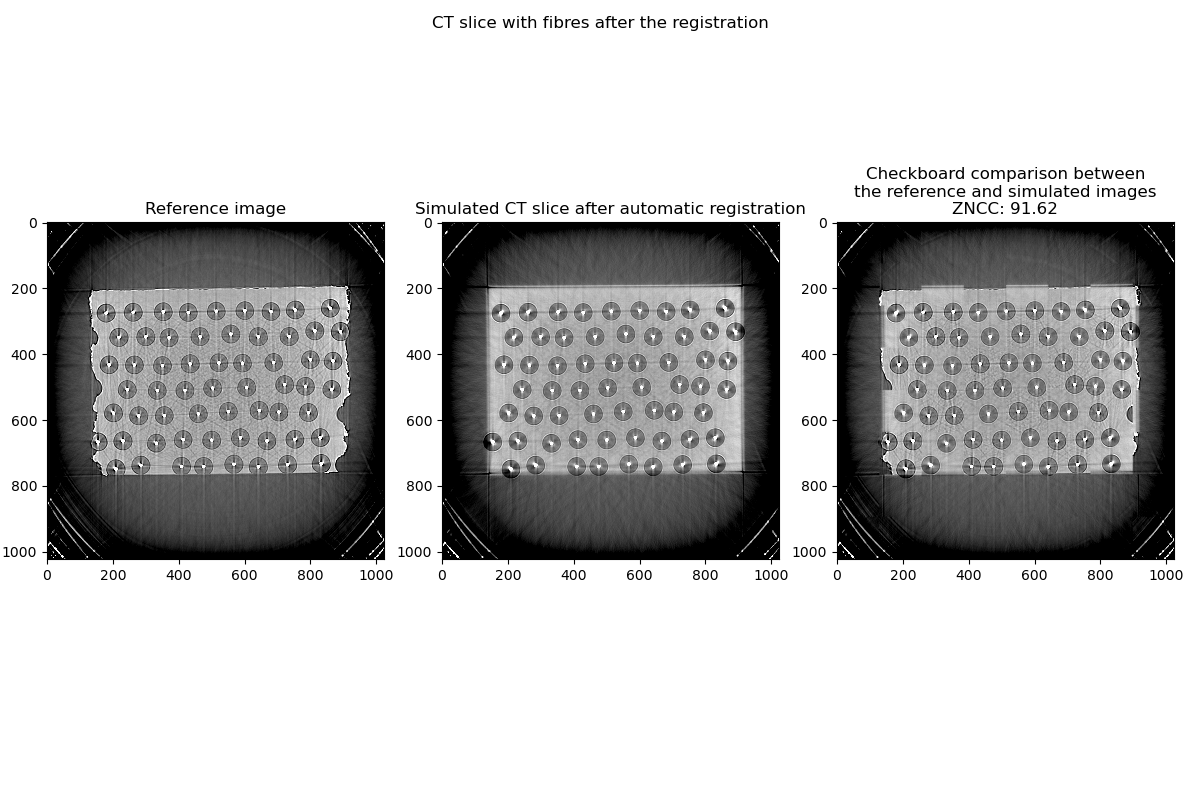
\includegraphics{plots/Fibre_in_centre_CT_slices_after_noise.png}
\caption{CT slice with fibres after the registration}
\end{figure}

    \begin{tcolorbox}[breakable, size=fbox, boxrule=1pt, pad at break*=1mm,colback=cellbackground, colframe=cellborder]
\prompt{In}{incolor}{98}{\boxspacing}
\begin{Verbatim}[commandchars=\\\{\}]
\PY{n}{test\PYZus{}fibre\PYZus{}in\PYZus{}centre}      \PY{o}{=} \PY{n}{np}\PY{o}{.}\PY{n}{array}\PY{p}{(}\PY{n}{copy}\PY{o}{.}\PY{n}{deepcopy}\PY{p}{(}\PY{n}{simulated\PYZus{}CT}\PY{p}{[}\PY{n}{cylinder\PYZus{}position\PYZus{}in\PYZus{}centre\PYZus{}of\PYZus{}slice}\PY{p}{[}\PY{l+m+mi}{1}\PY{p}{]} \PY{o}{\PYZhy{}} \PY{n}{roi\PYZus{}length}\PY{p}{:}\PY{n}{cylinder\PYZus{}position\PYZus{}in\PYZus{}centre\PYZus{}of\PYZus{}slice}\PY{p}{[}\PY{l+m+mi}{1}\PY{p}{]} \PY{o}{+} \PY{n}{roi\PYZus{}length}\PY{p}{,} \PY{n}{cylinder\PYZus{}position\PYZus{}in\PYZus{}centre\PYZus{}of\PYZus{}slice}\PY{p}{[}\PY{l+m+mi}{0}\PY{p}{]} \PY{o}{\PYZhy{}} \PY{n}{roi\PYZus{}length}\PY{p}{:}\PY{n}{cylinder\PYZus{}position\PYZus{}in\PYZus{}centre\PYZus{}of\PYZus{}slice}\PY{p}{[}\PY{l+m+mi}{0}\PY{p}{]} \PY{o}{+} \PY{n}{roi\PYZus{}length}\PY{p}{]}\PY{p}{)}\PY{p}{)}\PY{p}{;}
\PY{n}{profile\PYZus{}test\PYZus{}with\PYZus{}Poisson\PYZus{}noise} \PY{o}{=} \PY{n}{copy}\PY{o}{.}\PY{n}{deepcopy}\PY{p}{(}\PY{n}{np}\PY{o}{.}\PY{n}{diag}\PY{p}{(}\PY{n}{test\PYZus{}fibre\PYZus{}in\PYZus{}centre}\PY{p}{)}\PY{p}{)}\PY{p}{;}

\PY{n}{plt}\PY{o}{.}\PY{n}{figure}\PY{p}{(}\PY{p}{)}

\PY{n}{plt}\PY{o}{.}\PY{n}{title}\PY{p}{(}\PY{l+s+s2}{\PYZdq{}}\PY{l+s+s2}{Diagonal profile of the fibre in the centre of the reference CT and}\PY{l+s+se}{\PYZbs{}n}\PY{l+s+s2}{the simulated CT slice without and with Poisson noise}\PY{l+s+s2}{\PYZdq{}}\PY{p}{)}
\PY{n}{plt}\PY{o}{.}\PY{n}{plot}\PY{p}{(}\PY{n}{profile\PYZus{}reference}\PY{p}{,} \PY{n}{label}\PY{o}{=}\PY{l+s+s2}{\PYZdq{}}\PY{l+s+s2}{Reference}\PY{l+s+s2}{\PYZdq{}}\PY{p}{)}\PY{p}{;}
\PY{n}{plt}\PY{o}{.}\PY{n}{plot}\PY{p}{(}\PY{n}{profile\PYZus{}test\PYZus{}without\PYZus{}Poisson\PYZus{}noise}\PY{p}{,} \PY{n}{label}\PY{o}{=}\PY{l+s+s2}{\PYZdq{}}\PY{l+s+s2}{Simulation without Poisson noise}\PY{l+s+s2}{\PYZdq{}}\PY{p}{)}\PY{p}{;}
\PY{n}{plt}\PY{o}{.}\PY{n}{plot}\PY{p}{(}\PY{n}{profile\PYZus{}test\PYZus{}with\PYZus{}Poisson\PYZus{}noise}\PY{p}{,} \PY{n}{label}\PY{o}{=}\PY{l+s+s2}{\PYZdq{}}\PY{l+s+s2}{Simulation with Poisson noise}\PY{l+s+s2}{\PYZdq{}}\PY{p}{)}\PY{p}{;}
\PY{n}{plt}\PY{o}{.}\PY{n}{legend}\PY{p}{(}\PY{p}{)}\PY{p}{;}

\PY{n}{plt}\PY{o}{.}\PY{n}{savefig}\PY{p}{(}\PY{l+s+s1}{\PYZsq{}}\PY{l+s+s1}{plots/profiles.pdf}\PY{l+s+s1}{\PYZsq{}}\PY{p}{)}\PY{p}{;}
\PY{n}{plt}\PY{o}{.}\PY{n}{savefig}\PY{p}{(}\PY{l+s+s1}{\PYZsq{}}\PY{l+s+s1}{plots/profiles.png}\PY{l+s+s1}{\PYZsq{}}\PY{p}{)}\PY{p}{;}
\end{Verbatim}
\end{tcolorbox}

    \begin{figure}
\centering
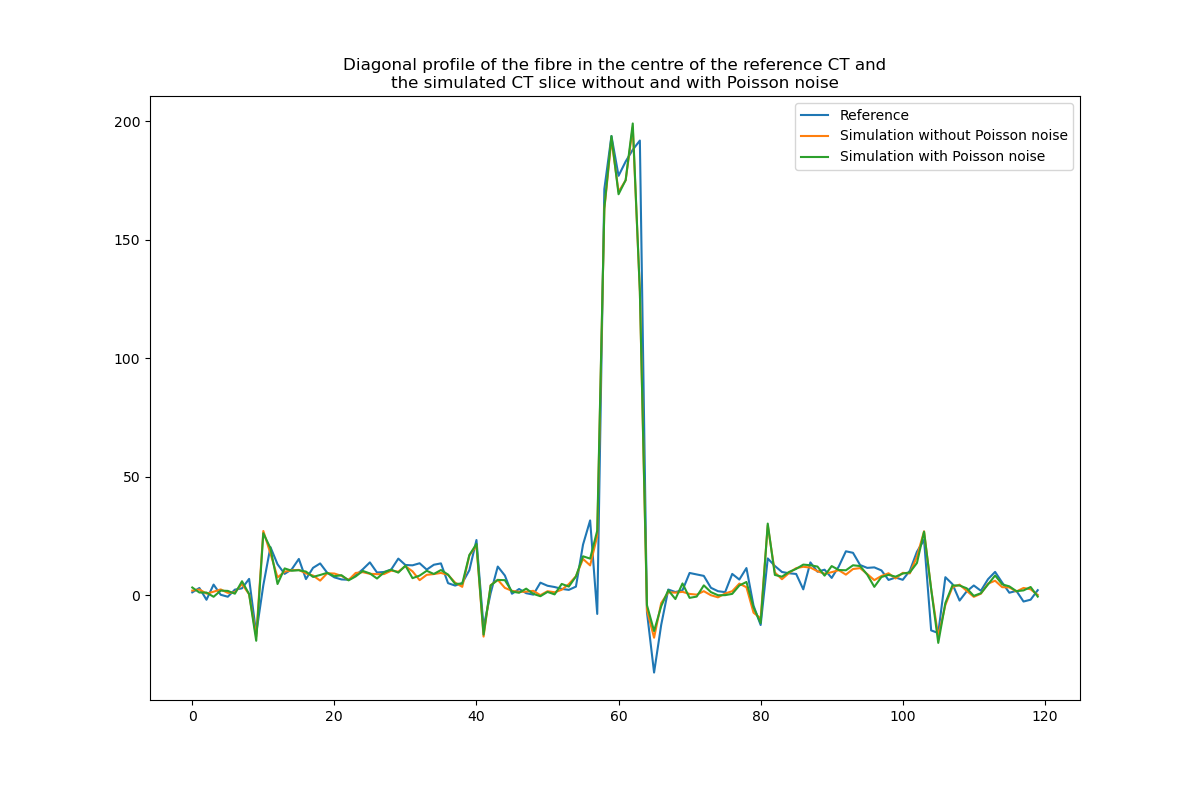
\includegraphics{plots/profiles.png}
\caption{Diagonal profile of the fibre in the centre of the reference
CT}
\end{figure}

\hypertarget{results-in-terms-of-linear-attenuation-coefficients}{%
\section{Results in terms of linear attenuation
coefficients}\label{results-in-terms-of-linear-attenuation-coefficients}}

    Reduce the ROI size to focus on a single fibre and its surrounding
matrix

    \begin{tcolorbox}[breakable, size=fbox, boxrule=1pt, pad at break*=1mm,colback=cellbackground, colframe=cellborder]
\prompt{In}{incolor}{99}{\boxspacing}
\begin{Verbatim}[commandchars=\\\{\}]
\PY{n}{roi\PYZus{}length} \PY{o}{=} \PY{l+m+mi}{40}
\end{Verbatim}
\end{tcolorbox}

    Extract the ROIs

    \begin{tcolorbox}[breakable, size=fbox, boxrule=1pt, pad at break*=1mm,colback=cellbackground, colframe=cellborder]
\prompt{In}{incolor}{100}{\boxspacing}
\begin{Verbatim}[commandchars=\\\{\}]
\PY{n}{reference\PYZus{}fibre\PYZus{}in\PYZus{}centre} \PY{o}{=} \PY{n}{np}\PY{o}{.}\PY{n}{array}\PY{p}{(}\PY{n}{copy}\PY{o}{.}\PY{n}{deepcopy}\PY{p}{(}\PY{n}{reference\PYZus{}CT}\PY{p}{[}\PY{n}{cylinder\PYZus{}position\PYZus{}in\PYZus{}centre\PYZus{}of\PYZus{}slice}\PY{p}{[}\PY{l+m+mi}{1}\PY{p}{]} \PY{o}{\PYZhy{}} \PY{n}{roi\PYZus{}length}\PY{p}{:}\PY{n}{cylinder\PYZus{}position\PYZus{}in\PYZus{}centre\PYZus{}of\PYZus{}slice}\PY{p}{[}\PY{l+m+mi}{1}\PY{p}{]} \PY{o}{+} \PY{n}{roi\PYZus{}length}\PY{p}{,} \PY{n}{cylinder\PYZus{}position\PYZus{}in\PYZus{}centre\PYZus{}of\PYZus{}slice}\PY{p}{[}\PY{l+m+mi}{0}\PY{p}{]} \PY{o}{\PYZhy{}} \PY{n}{roi\PYZus{}length}\PY{p}{:}\PY{n}{cylinder\PYZus{}position\PYZus{}in\PYZus{}centre\PYZus{}of\PYZus{}slice}\PY{p}{[}\PY{l+m+mi}{0}\PY{p}{]} \PY{o}{+} \PY{n}{roi\PYZus{}length}\PY{p}{]}\PY{p}{)}\PY{p}{)}\PY{p}{;}
\PY{n}{test\PYZus{}fibre\PYZus{}in\PYZus{}centre} \PY{o}{=} \PY{n}{np}\PY{o}{.}\PY{n}{array}\PY{p}{(}\PY{n}{copy}\PY{o}{.}\PY{n}{deepcopy}\PY{p}{(}\PY{n}{simulated\PYZus{}CT}\PY{p}{[}\PY{n}{cylinder\PYZus{}position\PYZus{}in\PYZus{}centre\PYZus{}of\PYZus{}slice}\PY{p}{[}\PY{l+m+mi}{1}\PY{p}{]} \PY{o}{\PYZhy{}} \PY{n}{roi\PYZus{}length}\PY{p}{:}\PY{n}{cylinder\PYZus{}position\PYZus{}in\PYZus{}centre\PYZus{}of\PYZus{}slice}\PY{p}{[}\PY{l+m+mi}{1}\PY{p}{]} \PY{o}{+} \PY{n}{roi\PYZus{}length}\PY{p}{,} \PY{n}{cylinder\PYZus{}position\PYZus{}in\PYZus{}centre\PYZus{}of\PYZus{}slice}\PY{p}{[}\PY{l+m+mi}{0}\PY{p}{]} \PY{o}{\PYZhy{}} \PY{n}{roi\PYZus{}length}\PY{p}{:}\PY{n}{cylinder\PYZus{}position\PYZus{}in\PYZus{}centre\PYZus{}of\PYZus{}slice}\PY{p}{[}\PY{l+m+mi}{0}\PY{p}{]} \PY{o}{+} \PY{n}{roi\PYZus{}length}\PY{p}{]}\PY{p}{)}\PY{p}{)}\PY{p}{;}
\end{Verbatim}
\end{tcolorbox}

    Save the ROIs

    \begin{tcolorbox}[breakable, size=fbox, boxrule=1pt, pad at break*=1mm,colback=cellbackground, colframe=cellborder]
\prompt{In}{incolor}{101}{\boxspacing}
\begin{Verbatim}[commandchars=\\\{\}]
\PY{n}{saveMHA}\PY{p}{(}\PY{l+s+s2}{\PYZdq{}}\PY{l+s+s2}{outputs/reference\PYZus{}fibre\PYZus{}in\PYZus{}centre.mha}\PY{l+s+s2}{\PYZdq{}}\PY{p}{,} \PY{n}{reference\PYZus{}fibre\PYZus{}in\PYZus{}centre}\PY{p}{,} \PY{p}{[}\PY{n}{pixel\PYZus{}spacing\PYZus{}in\PYZus{}mm}\PY{p}{,} \PY{n}{pixel\PYZus{}spacing\PYZus{}in\PYZus{}mm}\PY{p}{]}\PY{p}{)}\PY{p}{;}
\PY{n}{saveMHA}\PY{p}{(}\PY{l+s+s2}{\PYZdq{}}\PY{l+s+s2}{outputs/test\PYZus{}fibre\PYZus{}in\PYZus{}centre.mha}\PY{l+s+s2}{\PYZdq{}}\PY{p}{,} \PY{n}{test\PYZus{}fibre\PYZus{}in\PYZus{}centre}\PY{p}{,} \PY{p}{[}\PY{n}{pixel\PYZus{}spacing\PYZus{}in\PYZus{}mm}\PY{p}{,} \PY{n}{pixel\PYZus{}spacing\PYZus{}in\PYZus{}mm}\PY{p}{]}\PY{p}{)}\PY{p}{;}
\end{Verbatim}
\end{tcolorbox}

    A function to create a circular binary mask

    \begin{tcolorbox}[breakable, size=fbox, boxrule=1pt, pad at break*=1mm,colback=cellbackground, colframe=cellborder]
\prompt{In}{incolor}{102}{\boxspacing}
\begin{Verbatim}[commandchars=\\\{\}]
\PY{k}{def} \PY{n+nf}{create\PYZus{}circular\PYZus{}mask}\PY{p}{(}\PY{n}{h}\PY{p}{,} \PY{n}{w}\PY{p}{,} \PY{n}{center}\PY{o}{=}\PY{k+kc}{None}\PY{p}{,} \PY{n}{radius}\PY{o}{=}\PY{k+kc}{None}\PY{p}{)}\PY{p}{:}

    \PY{k}{if} \PY{n}{center} \PY{o+ow}{is} \PY{k+kc}{None}\PY{p}{:} \PY{c+c1}{\PYZsh{} use the middle of the image}
        \PY{n}{center} \PY{o}{=} \PY{p}{(}\PY{n+nb}{int}\PY{p}{(}\PY{n}{w}\PY{o}{/}\PY{l+m+mi}{2}\PY{p}{)}\PY{p}{,} \PY{n+nb}{int}\PY{p}{(}\PY{n}{h}\PY{o}{/}\PY{l+m+mi}{2}\PY{p}{)}\PY{p}{)}
    \PY{k}{if} \PY{n}{radius} \PY{o+ow}{is} \PY{k+kc}{None}\PY{p}{:} \PY{c+c1}{\PYZsh{} use the smallest distance between the center and image walls}
        \PY{n}{radius} \PY{o}{=} \PY{n+nb}{min}\PY{p}{(}\PY{n}{center}\PY{p}{[}\PY{l+m+mi}{0}\PY{p}{]}\PY{p}{,} \PY{n}{center}\PY{p}{[}\PY{l+m+mi}{1}\PY{p}{]}\PY{p}{,} \PY{n}{w}\PY{o}{\PYZhy{}}\PY{n}{center}\PY{p}{[}\PY{l+m+mi}{0}\PY{p}{]}\PY{p}{,} \PY{n}{h}\PY{o}{\PYZhy{}}\PY{n}{center}\PY{p}{[}\PY{l+m+mi}{1}\PY{p}{]}\PY{p}{)}

    \PY{n}{Y}\PY{p}{,} \PY{n}{X} \PY{o}{=} \PY{n}{np}\PY{o}{.}\PY{n}{ogrid}\PY{p}{[}\PY{p}{:}\PY{n}{h}\PY{p}{,} \PY{p}{:}\PY{n}{w}\PY{p}{]}
    \PY{n}{dist\PYZus{}from\PYZus{}center} \PY{o}{=} \PY{n}{np}\PY{o}{.}\PY{n}{sqrt}\PY{p}{(}\PY{p}{(}\PY{n}{X} \PY{o}{\PYZhy{}} \PY{n}{center}\PY{p}{[}\PY{l+m+mi}{0}\PY{p}{]}\PY{p}{)}\PY{o}{*}\PY{o}{*}\PY{l+m+mi}{2} \PY{o}{+} \PY{p}{(}\PY{n}{Y}\PY{o}{\PYZhy{}}\PY{n}{center}\PY{p}{[}\PY{l+m+mi}{1}\PY{p}{]}\PY{p}{)}\PY{o}{*}\PY{o}{*}\PY{l+m+mi}{2}\PY{p}{)}

    \PY{n}{mask} \PY{o}{=} \PY{n}{dist\PYZus{}from\PYZus{}center} \PY{o}{\PYZlt{}}\PY{o}{=} \PY{n}{radius}
    \PY{k}{return} \PY{n}{np}\PY{o}{.}\PY{n}{array}\PY{p}{(}\PY{n}{mask}\PY{p}{,} \PY{n}{dtype}\PY{o}{=}\PY{n+nb}{bool}\PY{p}{)}\PY{p}{;}
\end{Verbatim}
\end{tcolorbox}

    A function to create the binary masks for the core, fibre and matrix

    \begin{tcolorbox}[breakable, size=fbox, boxrule=1pt, pad at break*=1mm,colback=cellbackground, colframe=cellborder]
\prompt{In}{incolor}{103}{\boxspacing}
\begin{Verbatim}[commandchars=\\\{\}]
\PY{k}{def} \PY{n+nf}{createMasks}\PY{p}{(}\PY{n}{mask\PYZus{}shape}\PY{p}{)}\PY{p}{:}
    \PY{n}{fibre\PYZus{}radius\PYZus{}in\PYZus{}px} \PY{o}{=} \PY{n}{fibre\PYZus{}radius} \PY{o}{/} \PY{n}{pixel\PYZus{}spacing\PYZus{}in\PYZus{}micrometre}
    \PY{n}{core\PYZus{}radius\PYZus{}in\PYZus{}px} \PY{o}{=} \PY{n}{core\PYZus{}radius} \PY{o}{/} \PY{n}{pixel\PYZus{}spacing\PYZus{}in\PYZus{}micrometre}

    \PY{n}{core\PYZus{}mask} \PY{o}{=} \PY{n}{create\PYZus{}circular\PYZus{}mask}\PY{p}{(}\PY{n}{mask\PYZus{}shape}\PY{p}{[}\PY{l+m+mi}{1}\PY{p}{]}\PY{p}{,} \PY{n}{mask\PYZus{}shape}\PY{p}{[}\PY{l+m+mi}{0}\PY{p}{]}\PY{p}{,} \PY{k+kc}{None}\PY{p}{,} \PY{n}{core\PYZus{}radius\PYZus{}in\PYZus{}px}\PY{p}{)}\PY{p}{;}

    \PY{n}{fibre\PYZus{}mask} \PY{o}{=} \PY{n}{create\PYZus{}circular\PYZus{}mask}\PY{p}{(}\PY{n}{mask\PYZus{}shape}\PY{p}{[}\PY{l+m+mi}{1}\PY{p}{]}\PY{p}{,} \PY{n}{mask\PYZus{}shape}\PY{p}{[}\PY{l+m+mi}{0}\PY{p}{]}\PY{p}{,} \PY{k+kc}{None}\PY{p}{,} \PY{n}{fibre\PYZus{}radius\PYZus{}in\PYZus{}px}\PY{p}{)}\PY{p}{;}
    \PY{n}{matrix\PYZus{}mask} \PY{o}{=} \PY{n}{np}\PY{o}{.}\PY{n}{logical\PYZus{}not}\PY{p}{(}\PY{n}{fibre\PYZus{}mask}\PY{p}{)}\PY{p}{;}

    \PY{c+c1}{\PYZsh{}fibre\PYZus{}mask = np.subtract(fibre\PYZus{}mask, core\PYZus{}mask);}
    \PY{n}{fibre\PYZus{}mask} \PY{o}{=} \PY{n}{np}\PY{o}{.}\PY{n}{bitwise\PYZus{}xor}\PY{p}{(}\PY{n}{fibre\PYZus{}mask}\PY{p}{,} \PY{n}{core\PYZus{}mask}\PY{p}{)}\PY{p}{;}

    \PY{c+c1}{\PYZsh{}TypeError: numpy boolean subtract, the `\PYZhy{}` operator, is not supported, use the bitwise\PYZus{}xor, the `\PYZca{}` operator, or the logical\PYZus{}xor function instead.}

    \PY{k}{return} \PY{n}{core\PYZus{}mask}\PY{p}{,} \PY{n}{fibre\PYZus{}mask}\PY{p}{,} \PY{n}{matrix\PYZus{}mask}
\end{Verbatim}
\end{tcolorbox}

    Create binary masks for the core, fibre and matrix

    \begin{tcolorbox}[breakable, size=fbox, boxrule=1pt, pad at break*=1mm,colback=cellbackground, colframe=cellborder]
\prompt{In}{incolor}{104}{\boxspacing}
\begin{Verbatim}[commandchars=\\\{\}]
\PY{n}{mask\PYZus{}shape} \PY{o}{=} \PY{n}{reference\PYZus{}fibre\PYZus{}in\PYZus{}centre}\PY{o}{.}\PY{n}{shape}\PY{p}{;}
\PY{n}{core\PYZus{}mask}\PY{p}{,} \PY{n}{fibre\PYZus{}mask}\PY{p}{,} \PY{n}{matrix\PYZus{}mask} \PY{o}{=} \PY{n}{createMasks}\PY{p}{(}\PY{n}{mask\PYZus{}shape}\PY{p}{)}\PY{p}{;}

\PY{n}{core\PYZus{}mask} \PY{o}{=} \PY{n}{ndimage}\PY{o}{.}\PY{n}{binary\PYZus{}erosion}\PY{p}{(}\PY{n}{core\PYZus{}mask}\PY{p}{)}\PY{o}{.}\PY{n}{astype}\PY{p}{(}\PY{n}{core\PYZus{}mask}\PY{o}{.}\PY{n}{dtype}\PY{p}{)}\PY{p}{;}

\PY{k}{for} \PY{n}{i} \PY{o+ow}{in} \PY{n+nb}{range}\PY{p}{(}\PY{l+m+mi}{4}\PY{p}{)}\PY{p}{:}
    \PY{n}{fibre\PYZus{}mask} \PY{o}{=} \PY{n}{ndimage}\PY{o}{.}\PY{n}{binary\PYZus{}erosion}\PY{p}{(}\PY{n}{fibre\PYZus{}mask}\PY{p}{)}\PY{o}{.}\PY{n}{astype}\PY{p}{(}\PY{n}{fibre\PYZus{}mask}\PY{o}{.}\PY{n}{dtype}\PY{p}{)}\PY{p}{;}
    \PY{n}{matrix\PYZus{}mask} \PY{o}{=} \PY{n}{ndimage}\PY{o}{.}\PY{n}{binary\PYZus{}erosion}\PY{p}{(}\PY{n}{matrix\PYZus{}mask}\PY{p}{,} \PY{n}{border\PYZus{}value}\PY{o}{=}\PY{l+m+mi}{1}\PY{p}{)}\PY{o}{.}\PY{n}{astype}\PY{p}{(}\PY{n}{matrix\PYZus{}mask}\PY{o}{.}\PY{n}{dtype}\PY{p}{)}\PY{p}{;}

\PY{n}{core\PYZus{}mask}\PY{o}{.}\PY{n}{shape} \PY{o}{=} \PY{p}{[}\PY{n}{core\PYZus{}mask}\PY{o}{.}\PY{n}{shape}\PY{p}{[}\PY{l+m+mi}{0}\PY{p}{]}\PY{p}{,} \PY{n}{core\PYZus{}mask}\PY{o}{.}\PY{n}{shape}\PY{p}{[}\PY{l+m+mi}{1}\PY{p}{]}\PY{p}{]}
\PY{n}{fibre\PYZus{}mask}\PY{o}{.}\PY{n}{shape} \PY{o}{=} \PY{p}{[}\PY{n}{fibre\PYZus{}mask}\PY{o}{.}\PY{n}{shape}\PY{p}{[}\PY{l+m+mi}{0}\PY{p}{]}\PY{p}{,} \PY{n}{fibre\PYZus{}mask}\PY{o}{.}\PY{n}{shape}\PY{p}{[}\PY{l+m+mi}{1}\PY{p}{]}\PY{p}{]}
\PY{n}{matrix\PYZus{}mask}\PY{o}{.}\PY{n}{shape} \PY{o}{=} \PY{p}{[}\PY{n}{matrix\PYZus{}mask}\PY{o}{.}\PY{n}{shape}\PY{p}{[}\PY{l+m+mi}{0}\PY{p}{]}\PY{p}{,} \PY{n}{matrix\PYZus{}mask}\PY{o}{.}\PY{n}{shape}\PY{p}{[}\PY{l+m+mi}{1}\PY{p}{]}\PY{p}{]}
\end{Verbatim}
\end{tcolorbox}

    Save the binary masks

    \begin{tcolorbox}[breakable, size=fbox, boxrule=1pt, pad at break*=1mm,colback=cellbackground, colframe=cellborder]
\prompt{In}{incolor}{105}{\boxspacing}
\begin{Verbatim}[commandchars=\\\{\}]
\PY{n}{saveMHA}\PY{p}{(}\PY{l+s+s2}{\PYZdq{}}\PY{l+s+s2}{outputs/core\PYZus{}mask.mha}\PY{l+s+s2}{\PYZdq{}}\PY{p}{,} \PY{n}{core\PYZus{}mask}\PY{o}{.}\PY{n}{astype}\PY{p}{(}\PY{n}{np}\PY{o}{.}\PY{n}{uint8}\PY{p}{)}\PY{p}{,} \PY{p}{[}\PY{n}{pixel\PYZus{}spacing\PYZus{}in\PYZus{}mm}\PY{p}{,} \PY{n}{pixel\PYZus{}spacing\PYZus{}in\PYZus{}mm}\PY{p}{,} \PY{n}{pixel\PYZus{}spacing\PYZus{}in\PYZus{}mm}\PY{p}{]}\PY{p}{)}\PY{p}{;}
\PY{n}{saveMHA}\PY{p}{(}\PY{l+s+s2}{\PYZdq{}}\PY{l+s+s2}{outputs/fibre\PYZus{}mask.mha}\PY{l+s+s2}{\PYZdq{}}\PY{p}{,} \PY{n}{fibre\PYZus{}mask}\PY{o}{.}\PY{n}{astype}\PY{p}{(}\PY{n}{np}\PY{o}{.}\PY{n}{uint8}\PY{p}{)}\PY{p}{,} \PY{p}{[}\PY{n}{pixel\PYZus{}spacing\PYZus{}in\PYZus{}mm}\PY{p}{,} \PY{n}{pixel\PYZus{}spacing\PYZus{}in\PYZus{}mm}\PY{p}{,} \PY{n}{pixel\PYZus{}spacing\PYZus{}in\PYZus{}mm}\PY{p}{]}\PY{p}{)}\PY{p}{;}
\PY{n}{saveMHA}\PY{p}{(}\PY{l+s+s2}{\PYZdq{}}\PY{l+s+s2}{outputs/matrix\PYZus{}mask.mha}\PY{l+s+s2}{\PYZdq{}}\PY{p}{,} \PY{n}{matrix\PYZus{}mask}\PY{o}{.}\PY{n}{astype}\PY{p}{(}\PY{n}{np}\PY{o}{.}\PY{n}{uint8}\PY{p}{)}\PY{p}{,} \PY{p}{[}\PY{n}{pixel\PYZus{}spacing\PYZus{}in\PYZus{}mm}\PY{p}{,} \PY{n}{pixel\PYZus{}spacing\PYZus{}in\PYZus{}mm}\PY{p}{,} \PY{n}{pixel\PYZus{}spacing\PYZus{}in\PYZus{}mm}\PY{p}{]}\PY{p}{)}\PY{p}{;}
\end{Verbatim}
\end{tcolorbox}

    Display the masks

    \begin{tcolorbox}[breakable, size=fbox, boxrule=1pt, pad at break*=1mm,colback=cellbackground, colframe=cellborder]
\prompt{In}{incolor}{106}{\boxspacing}
\begin{Verbatim}[commandchars=\\\{\}]
\PY{n}{norm} \PY{o}{=} \PY{n}{cm}\PY{o}{.}\PY{n}{colors}\PY{o}{.}\PY{n}{Normalize}\PY{p}{(}\PY{n}{vmax}\PY{o}{=}\PY{l+m+mi}{1}\PY{p}{,} \PY{n}{vmin}\PY{o}{=}\PY{l+m+mi}{0}\PY{p}{)}

\PY{n}{fig}\PY{p}{,} \PY{p}{(}\PY{n}{ax1}\PY{p}{,} \PY{n}{ax2}\PY{p}{,} \PY{n}{ax3}\PY{p}{)} \PY{o}{=} \PY{n}{plt}\PY{o}{.}\PY{n}{subplots}\PY{p}{(}\PY{l+m+mi}{1}\PY{p}{,} \PY{l+m+mi}{3}\PY{p}{)}
\PY{n}{plt}\PY{o}{.}\PY{n}{tight\PYZus{}layout}\PY{p}{(}\PY{p}{)}
\PY{n}{fig}\PY{o}{.}\PY{n}{suptitle}\PY{p}{(}\PY{l+s+s1}{\PYZsq{}}\PY{l+s+s1}{Binary mask for every structure}\PY{l+s+s1}{\PYZsq{}}\PY{p}{)}

\PY{n}{ax1}\PY{o}{.}\PY{n}{set\PYZus{}title}\PY{p}{(}\PY{l+s+s2}{\PYZdq{}}\PY{l+s+s2}{W core}\PY{l+s+s2}{\PYZdq{}}\PY{p}{)}\PY{p}{;}
\PY{n}{imgplot1} \PY{o}{=} \PY{n}{ax1}\PY{o}{.}\PY{n}{imshow}\PY{p}{(}\PY{n}{core\PYZus{}mask}\PY{p}{,} \PY{n}{cmap}\PY{o}{=}\PY{l+s+s2}{\PYZdq{}}\PY{l+s+s2}{gray}\PY{l+s+s2}{\PYZdq{}}\PY{p}{,} 
                     \PY{n}{norm}\PY{o}{=}\PY{n}{norm}\PY{p}{)}\PY{p}{;}

\PY{n}{ax2}\PY{o}{.}\PY{n}{set\PYZus{}title}\PY{p}{(}\PY{l+s+s2}{\PYZdq{}}\PY{l+s+s2}{SiC fibre}\PY{l+s+s2}{\PYZdq{}}\PY{p}{)}\PY{p}{;}
\PY{n}{imgplot2} \PY{o}{=} \PY{n}{ax2}\PY{o}{.}\PY{n}{imshow}\PY{p}{(}\PY{n}{fibre\PYZus{}mask}\PY{p}{,}
                     \PY{n}{cmap}\PY{o}{=}\PY{l+s+s1}{\PYZsq{}}\PY{l+s+s1}{gray}\PY{l+s+s1}{\PYZsq{}}\PY{p}{,}
                     \PY{n}{norm}\PY{o}{=}\PY{n}{norm}\PY{p}{)}\PY{p}{;}

\PY{n}{ax3}\PY{o}{.}\PY{n}{set\PYZus{}title}\PY{p}{(}\PY{l+s+s2}{\PYZdq{}}\PY{l+s+s2}{Ti90Al6V4 matrix}\PY{l+s+s2}{\PYZdq{}}\PY{p}{)}\PY{p}{;}
\PY{n}{imgplot3} \PY{o}{=} \PY{n}{ax3}\PY{o}{.}\PY{n}{imshow}\PY{p}{(}\PY{n}{matrix\PYZus{}mask}\PY{p}{,}
                     \PY{n}{cmap}\PY{o}{=}\PY{l+s+s1}{\PYZsq{}}\PY{l+s+s1}{gray}\PY{l+s+s1}{\PYZsq{}}\PY{p}{,}
                     \PY{n}{norm}\PY{o}{=}\PY{n}{norm}\PY{p}{)}\PY{p}{;}

\PY{n}{plt}\PY{o}{.}\PY{n}{savefig}\PY{p}{(}\PY{l+s+s1}{\PYZsq{}}\PY{l+s+s1}{plots/masks.pdf}\PY{l+s+s1}{\PYZsq{}}\PY{p}{)}\PY{p}{;}
\PY{n}{plt}\PY{o}{.}\PY{n}{savefig}\PY{p}{(}\PY{l+s+s1}{\PYZsq{}}\PY{l+s+s1}{plots/masks.png}\PY{l+s+s1}{\PYZsq{}}\PY{p}{)}\PY{p}{;}
\end{Verbatim}
\end{tcolorbox}

    \begin{figure}
\centering
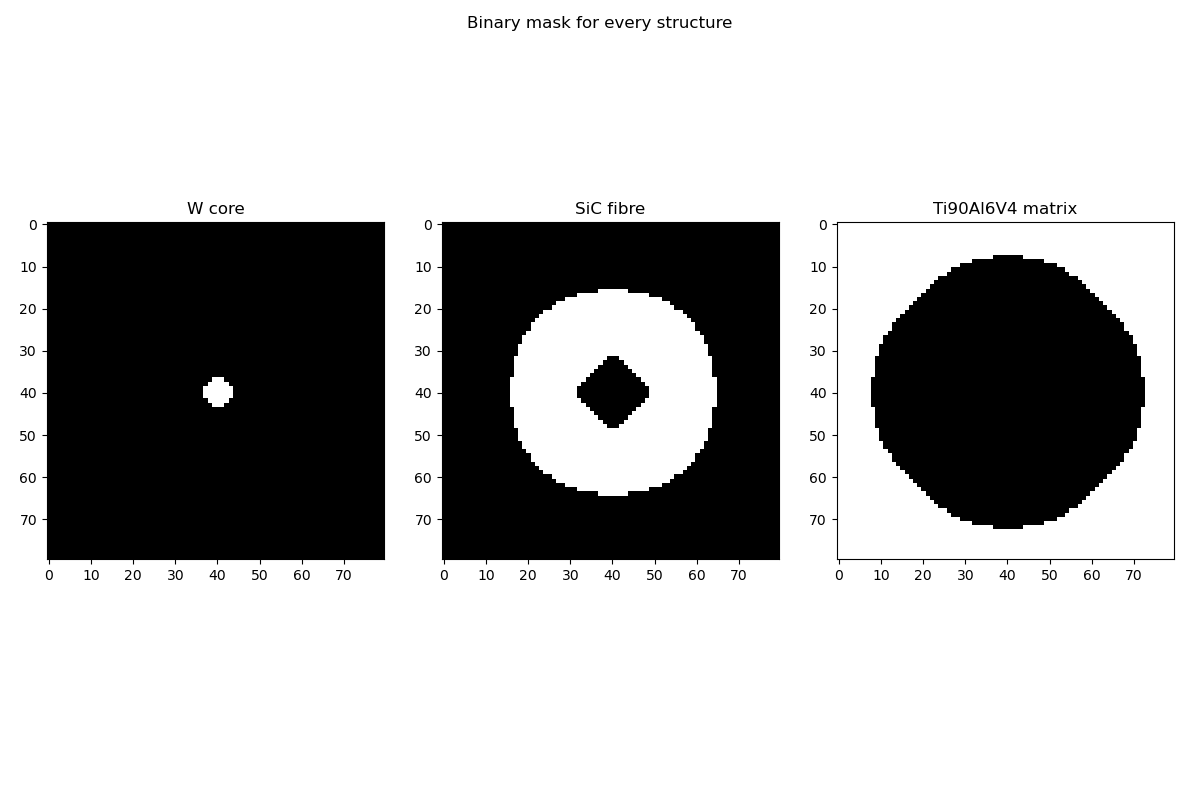
\includegraphics{plots/masks.png}
\caption{Binary mask for every structure}
\end{figure}

A function to collect all the \(\mu\) statistics from the masks.

    \begin{tcolorbox}[breakable, size=fbox, boxrule=1pt, pad at break*=1mm,colback=cellbackground, colframe=cellborder]
\prompt{In}{incolor}{107}{\boxspacing}
\begin{Verbatim}[commandchars=\\\{\}]
\PY{k}{def} \PY{n+nf}{getMuStatistics}\PY{p}{(}\PY{n}{reference\PYZus{}fibre\PYZus{}in\PYZus{}centre}\PY{p}{,} \PY{n}{test\PYZus{}fibre\PYZus{}in\PYZus{}centre}\PY{p}{,} \PY{n}{core\PYZus{}mask}\PY{p}{,} \PY{n}{fibre\PYZus{}mask}\PY{p}{,} \PY{n}{matrix\PYZus{}mask}\PY{p}{)}\PY{p}{:}

    \PY{n}{data} \PY{o}{=} \PY{p}{[}\PY{p}{]}\PY{p}{;}
    \PY{n}{index} \PY{o}{=} \PY{n}{np}\PY{o}{.}\PY{n}{nonzero}\PY{p}{(}\PY{n}{core\PYZus{}mask}\PY{p}{)}\PY{p}{;}
    
    \PY{n}{data}\PY{o}{.}\PY{n}{append}\PY{p}{(}\PY{p}{[}\PY{l+s+s2}{\PYZdq{}}\PY{l+s+s2}{Theorical}\PY{l+s+s2}{\PYZdq{}}\PY{p}{,} 
                \PY{l+s+s2}{\PYZdq{}}\PY{l+s+s2}{Core}\PY{l+s+s2}{\PYZdq{}}\PY{p}{,} 
                \PY{l+s+s2}{\PYZdq{}}\PY{l+s+s2}{W}\PY{l+s+s2}{\PYZdq{}}\PY{p}{,} 
                \PY{l+m+mf}{341.61}\PY{p}{,}
                \PY{l+m+mf}{341.61}\PY{p}{,}
                \PY{l+m+mf}{341.61}\PY{p}{,}
                \PY{l+m+mf}{0.0}\PY{p}{]}\PY{p}{)}\PY{p}{;}

    \PY{n}{data}\PY{o}{.}\PY{n}{append}\PY{p}{(}\PY{p}{[}\PY{l+s+s2}{\PYZdq{}}\PY{l+s+s2}{Experimental}\PY{l+s+s2}{\PYZdq{}}\PY{p}{,} 
                \PY{l+s+s2}{\PYZdq{}}\PY{l+s+s2}{Core}\PY{l+s+s2}{\PYZdq{}}\PY{p}{,} 
                \PY{l+s+s2}{\PYZdq{}}\PY{l+s+s2}{W}\PY{l+s+s2}{\PYZdq{}}\PY{p}{,} 
                \PY{n}{np}\PY{o}{.}\PY{n}{min}\PY{p}{(}\PY{n}{reference\PYZus{}fibre\PYZus{}in\PYZus{}centre}\PY{p}{[}\PY{n}{index}\PY{p}{]}\PY{p}{)}\PY{p}{,}
                \PY{n}{np}\PY{o}{.}\PY{n}{max}\PY{p}{(}\PY{n}{reference\PYZus{}fibre\PYZus{}in\PYZus{}centre}\PY{p}{[}\PY{n}{index}\PY{p}{]}\PY{p}{)}\PY{p}{,}
                \PY{n}{np}\PY{o}{.}\PY{n}{mean}\PY{p}{(}\PY{n}{reference\PYZus{}fibre\PYZus{}in\PYZus{}centre}\PY{p}{[}\PY{n}{index}\PY{p}{]}\PY{p}{)}\PY{p}{,}
                \PY{n}{np}\PY{o}{.}\PY{n}{std}\PY{p}{(}\PY{n}{reference\PYZus{}fibre\PYZus{}in\PYZus{}centre}\PY{p}{[}\PY{n}{index}\PY{p}{]}\PY{p}{)}\PY{p}{]}\PY{p}{)}\PY{p}{;}
    
    \PY{n}{data}\PY{o}{.}\PY{n}{append}\PY{p}{(}\PY{p}{[}\PY{l+s+s2}{\PYZdq{}}\PY{l+s+s2}{Simulated}\PY{l+s+s2}{\PYZdq{}}\PY{p}{,} 
                \PY{l+s+s2}{\PYZdq{}}\PY{l+s+s2}{Core}\PY{l+s+s2}{\PYZdq{}}\PY{p}{,} 
                \PY{l+s+s2}{\PYZdq{}}\PY{l+s+s2}{W}\PY{l+s+s2}{\PYZdq{}}\PY{p}{,} 
                \PY{n}{np}\PY{o}{.}\PY{n}{min}\PY{p}{(}\PY{n}{test\PYZus{}fibre\PYZus{}in\PYZus{}centre}\PY{p}{[}\PY{n}{index}\PY{p}{]}\PY{p}{)}\PY{p}{,}
                \PY{n}{np}\PY{o}{.}\PY{n}{max}\PY{p}{(}\PY{n}{test\PYZus{}fibre\PYZus{}in\PYZus{}centre}\PY{p}{[}\PY{n}{index}\PY{p}{]}\PY{p}{)}\PY{p}{,}
                \PY{n}{np}\PY{o}{.}\PY{n}{mean}\PY{p}{(}\PY{n}{test\PYZus{}fibre\PYZus{}in\PYZus{}centre}\PY{p}{[}\PY{n}{index}\PY{p}{]}\PY{p}{)}\PY{p}{,}
                \PY{n}{np}\PY{o}{.}\PY{n}{std}\PY{p}{(}\PY{n}{test\PYZus{}fibre\PYZus{}in\PYZus{}centre}\PY{p}{[}\PY{n}{index}\PY{p}{]}\PY{p}{)}\PY{p}{]}\PY{p}{)}\PY{p}{;}

    \PY{n}{index} \PY{o}{=} \PY{n}{np}\PY{o}{.}\PY{n}{nonzero}\PY{p}{(}\PY{n}{fibre\PYZus{}mask}\PY{p}{)}\PY{p}{;}

    \PY{n}{data}\PY{o}{.}\PY{n}{append}\PY{p}{(}\PY{p}{[}\PY{l+s+s2}{\PYZdq{}}\PY{l+s+s2}{Theorical}\PY{l+s+s2}{\PYZdq{}}\PY{p}{,} 
                \PY{l+s+s2}{\PYZdq{}}\PY{l+s+s2}{Fibre}\PY{l+s+s2}{\PYZdq{}}\PY{p}{,} 
                \PY{l+s+s2}{\PYZdq{}}\PY{l+s+s2}{SiC}\PY{l+s+s2}{\PYZdq{}}\PY{p}{,} 
                \PY{l+m+mf}{2.736}\PY{p}{,}
                \PY{l+m+mf}{2.736}\PY{p}{,}
                \PY{l+m+mf}{2.736}\PY{p}{,}
                \PY{l+m+mf}{0.0}\PY{p}{]}\PY{p}{)}\PY{p}{;}
    
    \PY{n}{data}\PY{o}{.}\PY{n}{append}\PY{p}{(}\PY{p}{[}\PY{l+s+s2}{\PYZdq{}}\PY{l+s+s2}{Experimental}\PY{l+s+s2}{\PYZdq{}}\PY{p}{,} 
                \PY{l+s+s2}{\PYZdq{}}\PY{l+s+s2}{Fibre}\PY{l+s+s2}{\PYZdq{}}\PY{p}{,} 
                \PY{l+s+s2}{\PYZdq{}}\PY{l+s+s2}{SiC}\PY{l+s+s2}{\PYZdq{}}\PY{p}{,} 
                \PY{n}{np}\PY{o}{.}\PY{n}{min}\PY{p}{(}\PY{n}{reference\PYZus{}fibre\PYZus{}in\PYZus{}centre}\PY{p}{[}\PY{n}{index}\PY{p}{]}\PY{p}{)}\PY{p}{,}
                \PY{n}{np}\PY{o}{.}\PY{n}{max}\PY{p}{(}\PY{n}{reference\PYZus{}fibre\PYZus{}in\PYZus{}centre}\PY{p}{[}\PY{n}{index}\PY{p}{]}\PY{p}{)}\PY{p}{,}
                \PY{n}{np}\PY{o}{.}\PY{n}{mean}\PY{p}{(}\PY{n}{reference\PYZus{}fibre\PYZus{}in\PYZus{}centre}\PY{p}{[}\PY{n}{index}\PY{p}{]}\PY{p}{)}\PY{p}{,}
                \PY{n}{np}\PY{o}{.}\PY{n}{std}\PY{p}{(}\PY{n}{reference\PYZus{}fibre\PYZus{}in\PYZus{}centre}\PY{p}{[}\PY{n}{index}\PY{p}{]}\PY{p}{)}\PY{p}{]}\PY{p}{)}\PY{p}{;}
    
    \PY{n}{data}\PY{o}{.}\PY{n}{append}\PY{p}{(}\PY{p}{[}\PY{l+s+s2}{\PYZdq{}}\PY{l+s+s2}{Simulated}\PY{l+s+s2}{\PYZdq{}}\PY{p}{,} 
                \PY{l+s+s2}{\PYZdq{}}\PY{l+s+s2}{Fibre}\PY{l+s+s2}{\PYZdq{}}\PY{p}{,} 
                \PY{l+s+s2}{\PYZdq{}}\PY{l+s+s2}{SiC}\PY{l+s+s2}{\PYZdq{}}\PY{p}{,} 
                \PY{n}{np}\PY{o}{.}\PY{n}{min}\PY{p}{(}\PY{n}{test\PYZus{}fibre\PYZus{}in\PYZus{}centre}\PY{p}{[}\PY{n}{index}\PY{p}{]}\PY{p}{)}\PY{p}{,}
                \PY{n}{np}\PY{o}{.}\PY{n}{max}\PY{p}{(}\PY{n}{test\PYZus{}fibre\PYZus{}in\PYZus{}centre}\PY{p}{[}\PY{n}{index}\PY{p}{]}\PY{p}{)}\PY{p}{,}
                \PY{n}{np}\PY{o}{.}\PY{n}{mean}\PY{p}{(}\PY{n}{test\PYZus{}fibre\PYZus{}in\PYZus{}centre}\PY{p}{[}\PY{n}{index}\PY{p}{]}\PY{p}{)}\PY{p}{,}
                \PY{n}{np}\PY{o}{.}\PY{n}{std}\PY{p}{(}\PY{n}{test\PYZus{}fibre\PYZus{}in\PYZus{}centre}\PY{p}{[}\PY{n}{index}\PY{p}{]}\PY{p}{)}\PY{p}{]}\PY{p}{)}\PY{p}{;}

    \PY{n}{index} \PY{o}{=} \PY{n}{np}\PY{o}{.}\PY{n}{nonzero}\PY{p}{(}\PY{n}{matrix\PYZus{}mask}\PY{p}{)}\PY{p}{;}
    \PY{n}{data}\PY{o}{.}\PY{n}{append}\PY{p}{(}\PY{p}{[}\PY{l+s+s2}{\PYZdq{}}\PY{l+s+s2}{Theorical}\PY{l+s+s2}{\PYZdq{}}\PY{p}{,} 
                \PY{l+s+s2}{\PYZdq{}}\PY{l+s+s2}{Matrix}\PY{l+s+s2}{\PYZdq{}}\PY{p}{,} 
                \PY{l+s+s2}{\PYZdq{}}\PY{l+s+s2}{Ti90Al6V4}\PY{l+s+s2}{\PYZdq{}}\PY{p}{,} 
                \PY{l+m+mf}{13.1274}\PY{p}{,}
                \PY{l+m+mf}{13.1274}\PY{p}{,}
                \PY{l+m+mf}{13.1274}\PY{p}{,}
                \PY{l+m+mf}{0.0}\PY{p}{]}\PY{p}{)}\PY{p}{;}

    \PY{n}{data}\PY{o}{.}\PY{n}{append}\PY{p}{(}\PY{p}{[}\PY{l+s+s2}{\PYZdq{}}\PY{l+s+s2}{Experimental}\PY{l+s+s2}{\PYZdq{}}\PY{p}{,} 
                \PY{l+s+s2}{\PYZdq{}}\PY{l+s+s2}{Matrix}\PY{l+s+s2}{\PYZdq{}}\PY{p}{,} 
                \PY{l+s+s2}{\PYZdq{}}\PY{l+s+s2}{Ti90Al6V4}\PY{l+s+s2}{\PYZdq{}}\PY{p}{,} 
                \PY{n}{np}\PY{o}{.}\PY{n}{min}\PY{p}{(}\PY{n}{reference\PYZus{}fibre\PYZus{}in\PYZus{}centre}\PY{p}{[}\PY{n}{index}\PY{p}{]}\PY{p}{)}\PY{p}{,}
                \PY{n}{np}\PY{o}{.}\PY{n}{max}\PY{p}{(}\PY{n}{reference\PYZus{}fibre\PYZus{}in\PYZus{}centre}\PY{p}{[}\PY{n}{index}\PY{p}{]}\PY{p}{)}\PY{p}{,}
                \PY{n}{np}\PY{o}{.}\PY{n}{mean}\PY{p}{(}\PY{n}{reference\PYZus{}fibre\PYZus{}in\PYZus{}centre}\PY{p}{[}\PY{n}{index}\PY{p}{]}\PY{p}{)}\PY{p}{,}
                \PY{n}{np}\PY{o}{.}\PY{n}{std}\PY{p}{(}\PY{n}{reference\PYZus{}fibre\PYZus{}in\PYZus{}centre}\PY{p}{[}\PY{n}{index}\PY{p}{]}\PY{p}{)}\PY{p}{]}\PY{p}{)}\PY{p}{;}
    
    \PY{n}{data}\PY{o}{.}\PY{n}{append}\PY{p}{(}\PY{p}{[}\PY{l+s+s2}{\PYZdq{}}\PY{l+s+s2}{Simulated}\PY{l+s+s2}{\PYZdq{}}\PY{p}{,} 
                \PY{l+s+s2}{\PYZdq{}}\PY{l+s+s2}{Matrix}\PY{l+s+s2}{\PYZdq{}}\PY{p}{,} 
                \PY{l+s+s2}{\PYZdq{}}\PY{l+s+s2}{Ti90Al6V4}\PY{l+s+s2}{\PYZdq{}}\PY{p}{,} 
                \PY{n}{np}\PY{o}{.}\PY{n}{min}\PY{p}{(}\PY{n}{test\PYZus{}fibre\PYZus{}in\PYZus{}centre}\PY{p}{[}\PY{n}{index}\PY{p}{]}\PY{p}{)}\PY{p}{,}
                \PY{n}{np}\PY{o}{.}\PY{n}{max}\PY{p}{(}\PY{n}{test\PYZus{}fibre\PYZus{}in\PYZus{}centre}\PY{p}{[}\PY{n}{index}\PY{p}{]}\PY{p}{)}\PY{p}{,}
                \PY{n}{np}\PY{o}{.}\PY{n}{mean}\PY{p}{(}\PY{n}{test\PYZus{}fibre\PYZus{}in\PYZus{}centre}\PY{p}{[}\PY{n}{index}\PY{p}{]}\PY{p}{)}\PY{p}{,}
                \PY{n}{np}\PY{o}{.}\PY{n}{std}\PY{p}{(}\PY{n}{test\PYZus{}fibre\PYZus{}in\PYZus{}centre}\PY{p}{[}\PY{n}{index}\PY{p}{]}\PY{p}{)}\PY{p}{]}\PY{p}{)}\PY{p}{;}
    
    \PY{k}{return} \PY{n}{pd}\PY{o}{.}\PY{n}{DataFrame}\PY{p}{(}\PY{n}{data}\PY{p}{,}
            \PY{n}{index}\PY{o}{=}\PY{k+kc}{None}\PY{p}{,}
            \PY{n}{columns}\PY{o}{=}\PY{p}{[}\PY{l+s+s1}{\PYZsq{}}\PY{l+s+s1}{CT}\PY{l+s+s1}{\PYZsq{}}\PY{p}{,} \PY{l+s+s1}{\PYZsq{}}\PY{l+s+s1}{Structure}\PY{l+s+s1}{\PYZsq{}}\PY{p}{,} \PY{l+s+s2}{\PYZdq{}}\PY{l+s+s2}{Composition}\PY{l+s+s2}{\PYZdq{}}\PY{p}{,} \PY{l+s+s1}{\PYZsq{}}\PY{l+s+s1}{min}\PY{l+s+s1}{\PYZsq{}}\PY{p}{,} \PY{l+s+s1}{\PYZsq{}}\PY{l+s+s1}{max}\PY{l+s+s1}{\PYZsq{}}\PY{p}{,} \PY{l+s+s1}{\PYZsq{}}\PY{l+s+s1}{mean}\PY{l+s+s1}{\PYZsq{}}\PY{p}{,} \PY{l+s+s1}{\PYZsq{}}\PY{l+s+s1}{stddev}\PY{l+s+s1}{\PYZsq{}}\PY{p}{]}\PY{p}{)}
\end{Verbatim}
\end{tcolorbox}

    Get the dataframe with all the values and display it as a table

    \begin{tcolorbox}[breakable, size=fbox, boxrule=1pt, pad at break*=1mm,colback=cellbackground, colframe=cellborder]
\prompt{In}{incolor}{108}{\boxspacing}
\begin{Verbatim}[commandchars=\\\{\}]
\PY{n}{df} \PY{o}{=} \PY{n}{getMuStatistics}\PY{p}{(}\PY{n}{reference\PYZus{}fibre\PYZus{}in\PYZus{}centre}\PY{p}{,} \PY{n}{test\PYZus{}fibre\PYZus{}in\PYZus{}centre}\PY{p}{,} \PY{n}{core\PYZus{}mask}\PY{p}{,} \PY{n}{fibre\PYZus{}mask}\PY{p}{,} \PY{n}{matrix\PYZus{}mask}\PY{p}{)}\PY{p}{;}

\PY{n}{display}\PY{p}{(}\PY{n}{df}\PY{p}{)}
\end{Verbatim}
\end{tcolorbox}

    
    \begin{Verbatim}[commandchars=\\\{\}]
             CT Structure Composition         min         max        mean  \textbackslash{}
0     Theorical      Core           W  341.610000  341.610000  341.610000   
1  Experimental      Core           W  120.325165  212.735718  188.644455   
2     Simulated      Core           W  119.220016  202.536987  179.626617   
3     Theorical     Fibre         SiC    2.736000    2.736000    2.736000   
4  Experimental     Fibre         SiC  -32.709011   31.958403    3.217891   
5     Simulated     Fibre         SiC  -19.739300   22.917288    2.364575   
6     Theorical    Matrix   Ti90Al6V4   13.127400   13.127400   13.127400   
7  Experimental    Matrix   Ti90Al6V4   -3.869796   25.127810   10.856583   
8     Simulated    Matrix   Ti90Al6V4   -1.814649   20.138229    9.487208   

      stddev  
0   0.000000  
1  16.044945  
2  16.344721  
3   0.000000  
4   6.269166  
5   4.345567  
6   0.000000  
7   4.368093  
8   3.306015  
    \end{Verbatim}

    
    \hypertarget{save-the-cad-models-and-plot-them-in-3d}{%
\section{Save the CAD models and plot them in
3D}\label{save-the-cad-models-and-plot-them-in-3d}}

    \begin{tcolorbox}[breakable, size=fbox, boxrule=1pt, pad at break*=1mm,colback=cellbackground, colframe=cellborder]
\prompt{In}{incolor}{109}{\boxspacing}
\begin{Verbatim}[commandchars=\\\{\}]
\PY{n}{gvxr}\PY{o}{.}\PY{n}{saveSTLfile}\PY{p}{(}\PY{l+s+s2}{\PYZdq{}}\PY{l+s+s2}{fibre}\PY{l+s+s2}{\PYZdq{}}\PY{p}{,} \PY{l+s+s2}{\PYZdq{}}\PY{l+s+s2}{outputs/final\PYZus{}SiC\PYZus{}fibres.stl}\PY{l+s+s2}{\PYZdq{}}\PY{p}{)}\PY{p}{;}
\PY{n}{gvxr}\PY{o}{.}\PY{n}{saveSTLfile}\PY{p}{(}\PY{l+s+s2}{\PYZdq{}}\PY{l+s+s2}{core}\PY{l+s+s2}{\PYZdq{}}\PY{p}{,}  \PY{l+s+s2}{\PYZdq{}}\PY{l+s+s2}{outputs/final\PYZus{}W\PYZus{}cores.stl}\PY{l+s+s2}{\PYZdq{}}\PY{p}{)}\PY{p}{;}
\PY{n}{gvxr}\PY{o}{.}\PY{n}{saveSTLfile}\PY{p}{(}\PY{l+s+s2}{\PYZdq{}}\PY{l+s+s2}{matrix}\PY{l+s+s2}{\PYZdq{}}\PY{p}{,} \PY{l+s+s2}{\PYZdq{}}\PY{l+s+s2}{outputs/final\PYZus{}Ti90Al6V4\PYZus{}matrix.stl}\PY{l+s+s2}{\PYZdq{}}\PY{p}{)}\PY{p}{;}
\end{Verbatim}
\end{tcolorbox}

    \begin{tcolorbox}[breakable, size=fbox, boxrule=1pt, pad at break*=1mm,colback=cellbackground, colframe=cellborder]
\prompt{In}{incolor}{110}{\boxspacing}
\begin{Verbatim}[commandchars=\\\{\}]
\PY{n}{np}\PY{o}{.}\PY{n}{savetxt}\PY{p}{(}\PY{l+s+s2}{\PYZdq{}}\PY{l+s+s2}{outputs/centroids.dat}\PY{l+s+s2}{\PYZdq{}}\PY{p}{,} \PY{n}{centroid\PYZus{}set}\PY{p}{)}\PY{p}{;}
\end{Verbatim}
\end{tcolorbox}

    Load the STL files

    \begin{tcolorbox}[breakable, size=fbox, boxrule=1pt, pad at break*=1mm,colback=cellbackground, colframe=cellborder]
\prompt{In}{incolor}{111}{\boxspacing}
\begin{Verbatim}[commandchars=\\\{\}]
\PY{n}{fibre\PYZus{}mesh} \PY{o}{=} \PY{n}{mesh}\PY{o}{.}\PY{n}{Mesh}\PY{o}{.}\PY{n}{from\PYZus{}file}\PY{p}{(}\PY{l+s+s1}{\PYZsq{}}\PY{l+s+s1}{outputs/final\PYZus{}SiC\PYZus{}fibres.stl}\PY{l+s+s1}{\PYZsq{}}\PY{p}{)}
\PY{n}{core\PYZus{}mesh} \PY{o}{=} \PY{n}{mesh}\PY{o}{.}\PY{n}{Mesh}\PY{o}{.}\PY{n}{from\PYZus{}file}\PY{p}{(}\PY{l+s+s1}{\PYZsq{}}\PY{l+s+s1}{outputs/final\PYZus{}W\PYZus{}cores.stl}\PY{l+s+s1}{\PYZsq{}}\PY{p}{)}
\PY{n}{matrix\PYZus{}mesh} \PY{o}{=} \PY{n}{mesh}\PY{o}{.}\PY{n}{Mesh}\PY{o}{.}\PY{n}{from\PYZus{}file}\PY{p}{(}\PY{l+s+s1}{\PYZsq{}}\PY{l+s+s1}{outputs/final\PYZus{}Ti90Al6V4\PYZus{}matrix.stl}\PY{l+s+s1}{\PYZsq{}}\PY{p}{)}
\end{Verbatim}
\end{tcolorbox}

    Fix their orientation for the 3D plot

    \begin{tcolorbox}[breakable, size=fbox, boxrule=1pt, pad at break*=1mm,colback=cellbackground, colframe=cellborder]
\prompt{In}{incolor}{112}{\boxspacing}
\begin{Verbatim}[commandchars=\\\{\}]
\PY{n}{fibre\PYZus{}mesh}\PY{o}{.}\PY{n}{rotate}\PY{p}{(}\PY{p}{[}\PY{l+m+mi}{1}\PY{p}{,} \PY{l+m+mf}{0.0}\PY{p}{,} \PY{l+m+mf}{0.0}\PY{p}{]}\PY{p}{,} \PY{n}{math}\PY{o}{.}\PY{n}{radians}\PY{p}{(}\PY{l+m+mi}{90}\PY{p}{)}\PY{p}{)}
\PY{n}{core\PYZus{}mesh}\PY{o}{.}\PY{n}{rotate}\PY{p}{(}\PY{p}{[}\PY{l+m+mi}{1}\PY{p}{,} \PY{l+m+mf}{0.0}\PY{p}{,} \PY{l+m+mf}{0.0}\PY{p}{]}\PY{p}{,} \PY{n}{math}\PY{o}{.}\PY{n}{radians}\PY{p}{(}\PY{l+m+mi}{90}\PY{p}{)}\PY{p}{)}
\PY{n}{matrix\PYZus{}mesh}\PY{o}{.}\PY{n}{rotate}\PY{p}{(}\PY{p}{[}\PY{l+m+mi}{1}\PY{p}{,} \PY{l+m+mf}{0.0}\PY{p}{,} \PY{l+m+mf}{0.0}\PY{p}{]}\PY{p}{,} \PY{n}{math}\PY{o}{.}\PY{n}{radians}\PY{p}{(}\PY{l+m+mi}{90}\PY{p}{)}\PY{p}{)}
\end{Verbatim}
\end{tcolorbox}

    Create a new plot

    \begin{tcolorbox}[breakable, size=fbox, boxrule=1pt, pad at break*=1mm,colback=cellbackground, colframe=cellborder]
\prompt{In}{incolor}{113}{\boxspacing}
\begin{Verbatim}[commandchars=\\\{\}]
\PY{n}{figure} \PY{o}{=} \PY{n}{plt}\PY{o}{.}\PY{n}{figure}\PY{p}{(}\PY{p}{)}
\PY{n}{axes} \PY{o}{=} \PY{n}{mplot3d}\PY{o}{.}\PY{n}{Axes3D}\PY{p}{(}\PY{n}{figure}\PY{p}{,} \PY{n}{azim}\PY{o}{=}\PY{l+m+mi}{30}\PY{p}{,} \PY{n}{elev}\PY{o}{=}\PY{l+m+mi}{40}\PY{p}{,} \PY{n}{auto\PYZus{}add\PYZus{}to\PYZus{}figure}\PY{o}{=}\PY{k+kc}{False}\PY{p}{)}
\PY{n}{figure}\PY{o}{.}\PY{n}{add\PYZus{}axes}\PY{p}{(}\PY{n}{axes}\PY{p}{)}
\end{Verbatim}
\end{tcolorbox}

            \begin{tcolorbox}[breakable, size=fbox, boxrule=.5pt, pad at break*=1mm, opacityfill=0]
\prompt{Out}{outcolor}{113}{\boxspacing}
\begin{Verbatim}[commandchars=\\\{\}]
<Axes3D:>
\end{Verbatim}
\end{tcolorbox}
        
    Add the vectors to the plot

    \begin{tcolorbox}[breakable, size=fbox, boxrule=1pt, pad at break*=1mm,colback=cellbackground, colframe=cellborder]
\prompt{In}{incolor}{114}{\boxspacing}
\begin{Verbatim}[commandchars=\\\{\}]
\PY{n}{axes}\PY{o}{.}\PY{n}{add\PYZus{}collection3d}\PY{p}{(}\PY{n}{mplot3d}\PY{o}{.}\PY{n}{art3d}\PY{o}{.}\PY{n}{Poly3DCollection}\PY{p}{(}\PY{n}{matrix\PYZus{}mesh}\PY{o}{.}\PY{n}{vectors}\PY{p}{,} \PY{n}{facecolors}\PY{o}{=}\PY{l+s+s1}{\PYZsq{}}\PY{l+s+s1}{\PYZsh{}7fc97f}\PY{l+s+s1}{\PYZsq{}}\PY{p}{,} \PY{n}{linewidths}\PY{o}{=}\PY{l+m+mi}{1}\PY{p}{,} \PY{n}{alpha}\PY{o}{=}\PY{l+m+mf}{0.1}\PY{p}{)}\PY{p}{)}
\PY{n}{axes}\PY{o}{.}\PY{n}{add\PYZus{}collection3d}\PY{p}{(}\PY{n}{mplot3d}\PY{o}{.}\PY{n}{art3d}\PY{o}{.}\PY{n}{Poly3DCollection}\PY{p}{(}\PY{n}{fibre\PYZus{}mesh}\PY{o}{.}\PY{n}{vectors}\PY{p}{,} \PY{n}{facecolors}\PY{o}{=}\PY{l+s+s1}{\PYZsq{}}\PY{l+s+s1}{\PYZsh{}beaed4}\PY{l+s+s1}{\PYZsq{}}\PY{p}{,} \PY{n}{linewidths}\PY{o}{=}\PY{l+m+mi}{1}\PY{p}{,} \PY{n}{alpha}\PY{o}{=}\PY{l+m+mf}{0.3}\PY{p}{)}\PY{p}{)}
\PY{n}{axes}\PY{o}{.}\PY{n}{add\PYZus{}collection3d}\PY{p}{(}\PY{n}{mplot3d}\PY{o}{.}\PY{n}{art3d}\PY{o}{.}\PY{n}{Poly3DCollection}\PY{p}{(}\PY{n}{core\PYZus{}mesh}\PY{o}{.}\PY{n}{vectors}\PY{p}{,} \PY{n}{facecolors}\PY{o}{=}\PY{l+s+s1}{\PYZsq{}}\PY{l+s+s1}{\PYZsh{}fdc086}\PY{l+s+s1}{\PYZsq{}}\PY{p}{,} \PY{n}{linewidths}\PY{o}{=}\PY{l+m+mi}{1}\PY{p}{,} \PY{n}{alpha}\PY{o}{=}\PY{l+m+mf}{1.0}\PY{p}{)}\PY{p}{)}
\end{Verbatim}
\end{tcolorbox}

            \begin{tcolorbox}[breakable, size=fbox, boxrule=.5pt, pad at break*=1mm, opacityfill=0]
\prompt{Out}{outcolor}{114}{\boxspacing}
\begin{Verbatim}[commandchars=\\\{\}]
<mpl\_toolkits.mplot3d.art3d.Poly3DCollection at 0x7f86181869a0>
\end{Verbatim}
\end{tcolorbox}
        
    Auto scale to the mesh size

    \begin{tcolorbox}[breakable, size=fbox, boxrule=1pt, pad at break*=1mm,colback=cellbackground, colframe=cellborder]
\prompt{In}{incolor}{115}{\boxspacing}
\begin{Verbatim}[commandchars=\\\{\}]
\PY{n}{scale} \PY{o}{=} \PY{n}{matrix\PYZus{}mesh}\PY{o}{.}\PY{n}{points}\PY{o}{.}\PY{n}{flatten}\PY{p}{(}\PY{p}{)}
\PY{n}{axes}\PY{o}{.}\PY{n}{auto\PYZus{}scale\PYZus{}xyz}\PY{p}{(}\PY{n}{scale}\PY{p}{,} \PY{n}{scale}\PY{p}{,} \PY{n}{scale}\PY{p}{)}
\end{Verbatim}
\end{tcolorbox}

    Save the figure

    \begin{tcolorbox}[breakable, size=fbox, boxrule=1pt, pad at break*=1mm,colback=cellbackground, colframe=cellborder]
\prompt{In}{incolor}{116}{\boxspacing}
\begin{Verbatim}[commandchars=\\\{\}]
\PY{n}{plt}\PY{o}{.}\PY{n}{title}\PY{p}{(}\PY{l+s+s2}{\PYZdq{}}\PY{l+s+s2}{Final CAD models (in mm)}\PY{l+s+s2}{\PYZdq{}}\PY{p}{)}\PY{p}{;}
\PY{n}{plt}\PY{o}{.}\PY{n}{savefig}\PY{p}{(}\PY{l+s+s1}{\PYZsq{}}\PY{l+s+s1}{plots/CAD\PYZus{}models.pdf}\PY{l+s+s1}{\PYZsq{}}\PY{p}{)}
\PY{n}{plt}\PY{o}{.}\PY{n}{savefig}\PY{p}{(}\PY{l+s+s1}{\PYZsq{}}\PY{l+s+s1}{plots/CAD\PYZus{}models.png}\PY{l+s+s1}{\PYZsq{}}\PY{p}{)}
\end{Verbatim}
\end{tcolorbox}

    \hypertarget{final-cad-models-in-mm}{%
\section{Final CAD models (in mm)}\label{final-cad-models-in-mm}}

\begin{figure}
\centering
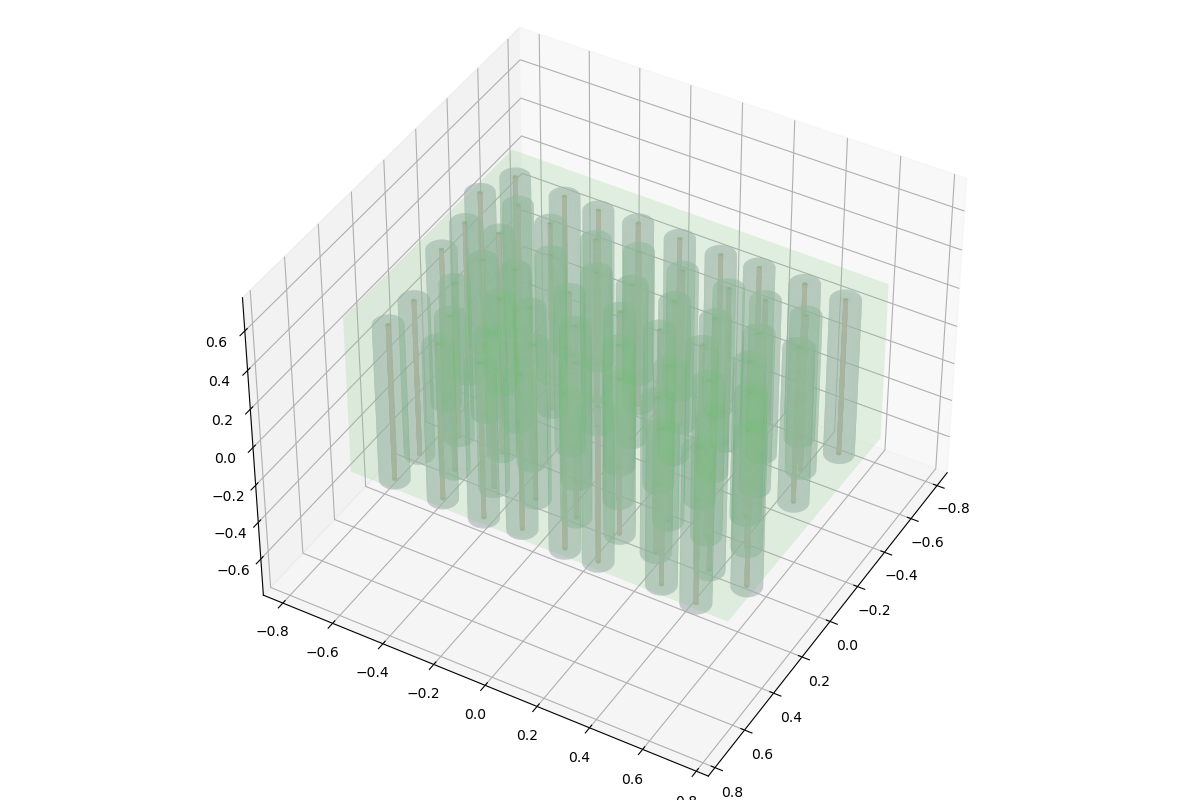
\includegraphics{./plots/CAD_models.png}
\caption{Final CAD models in 3D}
\end{figure}


    % Add a bibliography block to the postdoc
    
    
    
\end{document}
